% Options for packages loaded elsewhere
\PassOptionsToPackage{unicode}{hyperref}
\PassOptionsToPackage{hyphens}{url}
%
\documentclass[
  letterpaper,
  oneside,
  open=any]{scrbook}

\usepackage{amsmath,amssymb}
\usepackage{iftex}
\ifPDFTeX
  \usepackage[T1]{fontenc}
  \usepackage[utf8]{inputenc}
  \usepackage{textcomp} % provide euro and other symbols
\else % if luatex or xetex
  \usepackage{unicode-math}
  \defaultfontfeatures{Scale=MatchLowercase}
  \defaultfontfeatures[\rmfamily]{Ligatures=TeX,Scale=1}
\fi
\usepackage{lmodern}
\ifPDFTeX\else  
    % xetex/luatex font selection
\fi
% Use upquote if available, for straight quotes in verbatim environments
\IfFileExists{upquote.sty}{\usepackage{upquote}}{}
\IfFileExists{microtype.sty}{% use microtype if available
  \usepackage[]{microtype}
  \UseMicrotypeSet[protrusion]{basicmath} % disable protrusion for tt fonts
}{}
\makeatletter
\@ifundefined{KOMAClassName}{% if non-KOMA class
  \IfFileExists{parskip.sty}{%
    \usepackage{parskip}
  }{% else
    \setlength{\parindent}{0pt}
    \setlength{\parskip}{6pt plus 2pt minus 1pt}}
}{% if KOMA class
  \KOMAoptions{parskip=half}}
\makeatother
\usepackage{xcolor}
\setlength{\emergencystretch}{3em} % prevent overfull lines
\setcounter{secnumdepth}{5}
% Make \paragraph and \subparagraph free-standing
\makeatletter
\ifx\paragraph\undefined\else
  \let\oldparagraph\paragraph
  \renewcommand{\paragraph}{
    \@ifstar
      \xxxParagraphStar
      \xxxParagraphNoStar
  }
  \newcommand{\xxxParagraphStar}[1]{\oldparagraph*{#1}\mbox{}}
  \newcommand{\xxxParagraphNoStar}[1]{\oldparagraph{#1}\mbox{}}
\fi
\ifx\subparagraph\undefined\else
  \let\oldsubparagraph\subparagraph
  \renewcommand{\subparagraph}{
    \@ifstar
      \xxxSubParagraphStar
      \xxxSubParagraphNoStar
  }
  \newcommand{\xxxSubParagraphStar}[1]{\oldsubparagraph*{#1}\mbox{}}
  \newcommand{\xxxSubParagraphNoStar}[1]{\oldsubparagraph{#1}\mbox{}}
\fi
\makeatother

\providecommand{\tightlist}{%
  \setlength{\itemsep}{0pt}\setlength{\parskip}{0pt}}\usepackage{longtable,booktabs,array}
\usepackage{calc} % for calculating minipage widths
% Correct order of tables after \paragraph or \subparagraph
\usepackage{etoolbox}
\makeatletter
\patchcmd\longtable{\par}{\if@noskipsec\mbox{}\fi\par}{}{}
\makeatother
% Allow footnotes in longtable head/foot
\IfFileExists{footnotehyper.sty}{\usepackage{footnotehyper}}{\usepackage{footnote}}
\makesavenoteenv{longtable}
\usepackage{graphicx}
\makeatletter
\newsavebox\pandoc@box
\newcommand*\pandocbounded[1]{% scales image to fit in text height/width
  \sbox\pandoc@box{#1}%
  \Gscale@div\@tempa{\textheight}{\dimexpr\ht\pandoc@box+\dp\pandoc@box\relax}%
  \Gscale@div\@tempb{\linewidth}{\wd\pandoc@box}%
  \ifdim\@tempb\p@<\@tempa\p@\let\@tempa\@tempb\fi% select the smaller of both
  \ifdim\@tempa\p@<\p@\scalebox{\@tempa}{\usebox\pandoc@box}%
  \else\usebox{\pandoc@box}%
  \fi%
}
% Set default figure placement to htbp
\def\fps@figure{htbp}
\makeatother
% definitions for citeproc citations
\NewDocumentCommand\citeproctext{}{}
\NewDocumentCommand\citeproc{mm}{%
  \begingroup\def\citeproctext{#2}\cite{#1}\endgroup}
\makeatletter
 % allow citations to break across lines
 \let\@cite@ofmt\@firstofone
 % avoid brackets around text for \cite:
 \def\@biblabel#1{}
 \def\@cite#1#2{{#1\if@tempswa , #2\fi}}
\makeatother
\newlength{\cslhangindent}
\setlength{\cslhangindent}{1.5em}
\newlength{\csllabelwidth}
\setlength{\csllabelwidth}{3em}
\newenvironment{CSLReferences}[2] % #1 hanging-indent, #2 entry-spacing
 {\begin{list}{}{%
  \setlength{\itemindent}{0pt}
  \setlength{\leftmargin}{0pt}
  \setlength{\parsep}{0pt}
  % turn on hanging indent if param 1 is 1
  \ifodd #1
   \setlength{\leftmargin}{\cslhangindent}
   \setlength{\itemindent}{-1\cslhangindent}
  \fi
  % set entry spacing
  \setlength{\itemsep}{#2\baselineskip}}}
 {\end{list}}
\usepackage{calc}
\newcommand{\CSLBlock}[1]{\hfill\break\parbox[t]{\linewidth}{\strut\ignorespaces#1\strut}}
\newcommand{\CSLLeftMargin}[1]{\parbox[t]{\csllabelwidth}{\strut#1\strut}}
\newcommand{\CSLRightInline}[1]{\parbox[t]{\linewidth - \csllabelwidth}{\strut#1\strut}}
\newcommand{\CSLIndent}[1]{\hspace{\cslhangindent}#1}

\usepackage[default]{opensans}
\fontseries{lc}\selectfont
\makeatletter
\@ifpackageloaded{bookmark}{}{\usepackage{bookmark}}
\makeatother
\makeatletter
\@ifpackageloaded{caption}{}{\usepackage{caption}}
\AtBeginDocument{%
\ifdefined\contentsname
  \renewcommand*\contentsname{Table of contents}
\else
  \newcommand\contentsname{Table of contents}
\fi
\ifdefined\listfigurename
  \renewcommand*\listfigurename{List of Figures}
\else
  \newcommand\listfigurename{List of Figures}
\fi
\ifdefined\listtablename
  \renewcommand*\listtablename{List of Tables}
\else
  \newcommand\listtablename{List of Tables}
\fi
\ifdefined\figurename
  \renewcommand*\figurename{Figure}
\else
  \newcommand\figurename{Figure}
\fi
\ifdefined\tablename
  \renewcommand*\tablename{Table}
\else
  \newcommand\tablename{Table}
\fi
}
\@ifpackageloaded{float}{}{\usepackage{float}}
\floatstyle{ruled}
\@ifundefined{c@chapter}{\newfloat{codelisting}{h}{lop}}{\newfloat{codelisting}{h}{lop}[chapter]}
\floatname{codelisting}{Listing}
\newcommand*\listoflistings{\listof{codelisting}{List of Listings}}
\makeatother
\makeatletter
\makeatother
\makeatletter
\@ifpackageloaded{caption}{}{\usepackage{caption}}
\@ifpackageloaded{subcaption}{}{\usepackage{subcaption}}
\makeatother

\usepackage{hyphenat}
\usepackage{ifthen}
\usepackage{calc}
\usepackage{calculator}

\usepackage{graphicx}
\usepackage{wallpaper}

\usepackage{geometry}

\usepackage{graphicx}
\usepackage{geometry}
\usepackage{afterpage}
\usepackage{tikz}
\usetikzlibrary{calc}
\usetikzlibrary{fadings}
\usepackage[pagecolor=none]{pagecolor}


% Set the titlepage font families







% Set the coverpage font families


\usepackage{bookmark}

\IfFileExists{xurl.sty}{\usepackage{xurl}}{} % add URL line breaks if available
\urlstyle{same} % disable monospaced font for URLs
\hypersetup{
  pdftitle={Caribbean Ecosystem Status Report},
  pdfauthor={Southeast Integrated Ecosystem Assessment Program},
  hidelinks,
  pdfcreator={LaTeX via pandoc}}


\title{Caribbean Ecosystem Status Report}
\author{Southeast Integrated Ecosystem Assessment Program}
\date{2025-03-19}

\begin{document}
%%%%% begin titlepage extension code

  \begin{frontmatter}

\begin{titlepage}
% This is a combination of Pandoc templating and LaTeX
% Pandoc templating https://pandoc.org/MANUAL.html#templates
% See the README for help

\thispagestyle{empty}

\newgeometry{top=-100in}

% Page color

\newcommand{\coverauthorstyle}[1]{{\fontsize{20}{24.0}\selectfont
#1}}

\begin{tikzpicture}[remember picture, overlay, inner sep=0pt, outer sep=0pt]

\tikzfading[name=fadeout, inner color=transparent!0,outer color=transparent!100]
\tikzfading[name=fadein, inner color=transparent!100,outer color=transparent!0]
\node[anchor=south west, rotate=0.0, opacity=1.0] at ($(current page.south west)+(0pt, 8.75in)$) {

\includegraphics[width=\paperwidth, keepaspectratio]{images/cover-header-2.png}};

% Title
\newcommand{\titlelocationleft}{2.3in}
\newcommand{\titlelocationbottom}{7in}
\newcommand{\titlealign}{left}

\begin{scope}{%
\fontsize{30}{36.0}\selectfont
\node[anchor=north
west, align=left, rotate=0] (Title1) at ($(current page.south west)+(\titlelocationleft,\titlelocationbottom)$)  [text width = 5in]  {\textcolor{black}{\bfseries{\nohyphens{Caribbean
Ecosystem Status Report}}}};
}
\end{scope}

% Author
\newcommand{\authorlocationleft}{2.3in}
\newcommand{\authorlocationbottom}{5in}
\newcommand{\authoralign}{left}

\begin{scope}
{%
\fontsize{20}{24.0}\selectfont
\node[anchor=north
west, align=left, rotate=0] (Author1) at ($(current page.south west)+(\authorlocationleft,\authorlocationbottom)$)  [text width = 5in]  {
\coverauthorstyle{Southeast Integrated Ecosystem Assessment Program\\}};
}
\end{scope}

% Header
\newcommand{\headerlocationleft}{2.3in}
\newcommand{\headerlocationbottom}{9.8in}
\newcommand{\headerlocationalign}{left}

\begin{scope}
{%
\fontsize{16}{19.2}\selectfont
 \node[anchor=north west, align=left, rotate=0] (Header1) at %
($(current page.south west)+(\headerlocationleft,\headerlocationbottom)$)  [text width = 5in]  {\textcolor{white}{\nohyphens{NOAA
Technical Memorandum NMFS-XXX-\#\#}}};
}
\end{scope}

% Footer
\newcommand{\footerlocationleft}{6in}
\newcommand{\footerlocationbottom}{0.1\paperheight}
\newcommand{\footerlocationalign}{left}

\begin{scope}
{%
\fontsize{8}{9.6}\selectfont
 \node[anchor=north west, align=left, rotate=0] (Footer1) at %
($(current page.south west)+(\footerlocationleft,\footerlocationbottom)$)  [text width = 2.5in]  {{\nohyphens{U.S.
DEPARTMENT OF COMMERCE\\
\strut \\
National Oceanic and Atmospheric Administration\\
National Marine Fisheries Service\\
Northwest Fisheries Science Center}}};
}
\end{scope}

% Date
\newcommand{\datelocationleft}{6in}
\newcommand{\datelocationbottom}{2in}
\newcommand{\datelocationalign}{left}

\begin{scope}
{%
\fontsize{20}{24.0}\selectfont
 \node[anchor=north west, align=left, rotate=0] (Date1) at %
($(current page.south west)+(\datelocationleft,\datelocationbottom)$)  [text width = 2.5in]  {{\nohyphens{December
2024}}};
}
\end{scope}

\end{tikzpicture}
\clearpage
\restoregeometry
%%% TITLE PAGE START

% Set up alignment commands
%Page
\newcommand{\titlepagepagealign}{
\ifthenelse{\equal{left}{right}}{\raggedleft}{}
\ifthenelse{\equal{left}{center}}{\centering}{}
\ifthenelse{\equal{left}{left}}{\raggedright}{}
}
%% Titles
\newcommand{\titlepagetitlealign}{
\ifthenelse{\equal{left}{right}}{\raggedleft}{}
\ifthenelse{\equal{left}{center}}{\centering}{}
\ifthenelse{\equal{left}{left}}{\raggedright}{}
\ifthenelse{\equal{left}{spread}}{\makebox[\linewidth][s]}{}
}


\newcommand{\titleandsubtitle}{
% Title and subtitle
{\fontsize{30}{36.0}\selectfont
\textcolor{black}{\bfseries{\nohyphens{Caribbean Ecosystem Status
Report}}}\par
}%
}
\newcommand{\titlepagetitleblock}{
\titleandsubtitle
}

\newcommand{\authorstyle}[1]{{\fontsize{20}{24.0}\selectfont
#1}}

\newcommand{\affiliationstyle}[1]{{#1}}

\newcommand{\titlepageauthorblock}{
{\authorstyle{\nohyphens{Southeast Integrated Ecosystem Assessment
Program}{\textsuperscript{1}}}}}

\newcommand{\titlepageaffiliationblock}{
\hangindent=1em
\hangafter=1
{\affiliationstyle{
{1}.~NOAA Fisheres,~Southeast Fisheries Science Center


\vspace{1\baselineskip} 
}}
}
\newcommand{\headerstyled}{%
{}
}
\newcommand{\footerstyled}{%
{}
}
\newcommand{\datestyled}{%
{2025-03-19}
}


\newcommand{\titlepageheaderblock}{\headerstyled}

\newcommand{\titlepagefooterblock}{
\footerstyled
}

\newcommand{\titlepagedateblock}{
\datestyled
}

%set up blocks so user can specify order
\newcommand{\titleblock}{{\titlepagetitlealign

{\titlepagetitleblock}
}

\vspace{4\baselineskip}
}

\newcommand{\authorblock}{{\titlepageauthorblock}

\vspace{2\baselineskip}
}

\newcommand{\affiliationblock}{{\titlepageaffiliationblock}

\vspace{2\baselineskip}
}

\newcommand{\logoblock}{}

\newcommand{\footerblock}{}

\newcommand{\dateblock}{{\titlepagedateblock}

\vspace{0pt}
}

\newcommand{\headerblock}{}
\newgeometry{top=3in,bottom=1in,right=1in,left=1.75in}
% background image
\newlength{\bgimagesize}
\setlength{\bgimagesize}{0.75\paperwidth}
\LENGTHDIVIDE{\bgimagesize}{\paperwidth}{\theRatio} % from calculator pkg
\ThisULCornerWallPaper{\theRatio}{images/corner-image.png}

\thispagestyle{empty} % no page numbers on titlepages


\newcommand{\vrulecode}{\rule{\vrulewidth}{\textheight}}
\newlength{\vrulewidth}
\setlength{\vrulewidth}{0pt}
\newlength{\B}
\setlength{\B}{\ifdim\vrulewidth > 0pt 0.05\textwidth\else 0pt\fi}
\newlength{\minipagewidth}
\ifthenelse{\equal{left}{left} \OR \equal{left}{right} }
{% True case
\setlength{\minipagewidth}{\textwidth - \vrulewidth - \B - 0.1\textwidth}
}{
\setlength{\minipagewidth}{\textwidth - 2\vrulewidth - 2\B - 0.1\textwidth}
}
\ifthenelse{\equal{left}{left} \OR \equal{left}{leftright}}
{% True case
\raggedleft % needed for the minipage to work
\vrulecode
\hspace{\B}
}{%
\raggedright % else it is right only and width is not 0
}
% [position of box][box height][inner position]{width}
% [s] means stretch out vertically; assuming there is a vfill
\begin{minipage}[b][\textheight][s]{\minipagewidth}
\titlepagepagealign
\headerblock

\titleblock

\authorblock

\affiliationblock

\vfill

\logoblock

\footerblock
\par

\end{minipage}\ifthenelse{\equal{left}{right} \OR \equal{left}{leftright} }{
\hspace{\B}
\vrulecode}{}
\clearpage
\restoregeometry
%%% TITLE PAGE END
\end{titlepage}
\setcounter{page}{3}
\end{frontmatter}

%%%%% end titlepage extension code

\renewcommand*\contentsname{Table of contents}
{
\setcounter{tocdepth}{1}
\tableofcontents
}
\listoffigures

\mainmatter
\bookmarksetup{startatroot}

\chapter{Introduction}\label{introduction}

\section{About this report}\label{about-this-report}

The purpose of this report is to synthesize diverse information sources
to assist with implementation of ecosystem-based fisheries management in
the U.S. Caribbean region, which includes Puerto Rico and the U.S.
Virgin Islands (USVI). A suite of indicators that span physical,
biological, social and economic elements of the ecosystem are reported
with the goal of helping the Caribbean Fishery Management Council (CFMC)
and other resource managers measure progress toward fishery management
objectives. The report relied on both previously identified proposed
indicators and expert vetting to select a suite of indicators that best
address the fishery management plan (FMP) objectives for the U.S.
Caribbean. Information in this report is organized into two sections: 1)
tracking performance toward predefined fishery management objectives,
and 2) potential risks to meeting those fishery management objectives.

The first set of indicators can be used to consider progress toward
stated management objectives. Management objectives were gleaned from
the Island-based Fishery Management Plans and categorized into seven
groups: food production, socioeconomic health, equity, engagement and
participation, bycatch reduction, governance, and protection of
ecosystems. Each of these sections contains a selection of indicators
that can be used to better understand how well these respective
management objectives are being met. Note that for some indicators,
directionality can be associated with positive or negative progress
toward management objectives (e.g., increases in abundance of
economically important species is generally associated with improved
management). However for other indicators, directionality can be
considered neutral (e.g., proportion of diving trips, changes in
contribution to revenue), although changes in these indicators represent
important shifts in the fishing dynamics of which managers should be
aware. The risk indicator section quantifies major stressors (as
identified by stakeholders) that capture the potential risks to meeting
fishery management objectives. These indicators provide managers with an
understanding of the backdrop against which management is occurring.
Major changes in these indicators may be associated with decreased
effectiveness of fisheries management, if the influences of external
environmental or economic stressors are strong relative to influences
from adjustments in fishing activity.

This report was created in Quarto
(\url{https://github.com/quarto-dev/quarto-cli/}) using the NOAA Quarto
book template
(\hyperref[0]{https://github.com/nmfs-opensci/NOAA-quarto-book}). A
github repository houses all the indicator data and R code used to
compile the report
(\hyperref[0]{https://github.com/Gulf-IEA/Caribbean-ESR-2}).

\section{Indicator selection}\label{indicator-selection}

The CFMC's Science and Statistical Committee, as well as the region's
Ecosystem-Based Fishery Management Technical Advisory Panel (EBFM TAP),
recently completed a series of conceptual models linking key components
of the ecosystem and human activities related to fishing (Seara et al.
2024). This report used these conceptual models as a starting list of
proposed indicators and matched the indicators to answer FMP objectives
when possible. For those objectives that did not have an immediate
conceptual model-identified indicator, this report used a decision
matrix process for expert vetting (Figure~\ref{fig-flowchart}).

\begin{figure}

\centering{

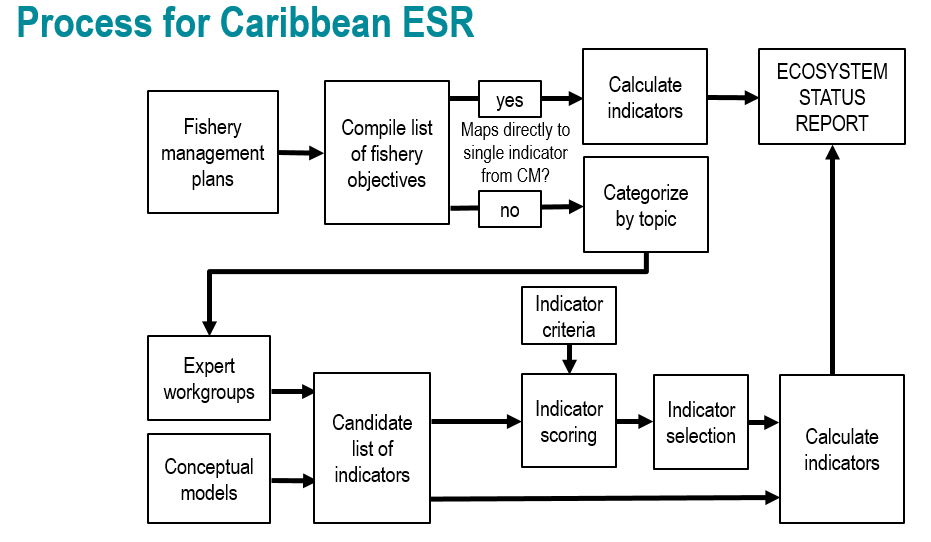
\includegraphics[width=5.36458in,height=\textheight,keepaspectratio]{images/process_flow_chart.png}

}

\caption{\label{fig-flowchart}Process for selecting indicators for the
U.S. Caribbean Ecosystem Status Report.}

\end{figure}%

This decision matrix was composed of a list of proposed indicators
compiled from the conceptual models as well as proposed indicators
provided via expert input. These potential indicators were vetted and
edited by expert small working groups, who then scored a decision matrix
of potential indicators (Montenero, Kelble, and Broughton 2021) against
the following decision criteria: long term data availability,
measurability, sensitivity to environmental changes, specificity,
spatial and temporal scalability, relevance to specific FMP objectives,
and responsiveness to management actions.

\section{Notes on interpreting time series
figures}\label{notes-on-interpreting-time-series-figures}

Time series data are plotted in a standardized format for ease of
interpretation (e.g., Figure~\ref{fig-explot}). The x-axis represents
the temporal dimension, which may be monthly, yearly, or irregular time
steps, and the y-axis represents the indicator value in units specified
in the axis label. Measures of uncertainty in the indicator values are
also shown, when available. The dashed horizontal line represents the
mean indicator value across the entire time series, and the solid
horizontal lines denote the mean plus or minus one standard deviation.
Red shaded areas and green shaded areas show years for which the
indicator value is below or above one standard deviation from the mean,
respectively. The blue vertical shaded box highlights the last five
years of indicator values, over which additional metrics are calculated.
Black circles to the right of each figure indicate whether the indicator
values over the last five years are greater (plus sign), less than
(minus sign), or within (solid circle) one standard deviation from the
mean of the overall time series. Arrows to the right of each figure
indicate whether the least squares linear fit through the last five
years of data produces a positive or negative slope that is greater than
one standard deviation (upward or downward arrows respectively), or less
than one standard deviation (left-right arrow).

\begin{figure}

\centering{

\pandocbounded{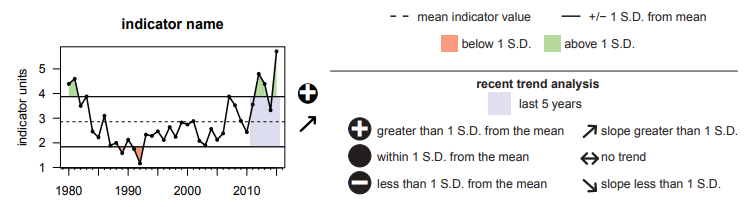
\includegraphics[keepaspectratio]{images/indicator_selection_diagram.png}}

}

\caption{\label{fig-explot}Example time series plot, showing an
indicator plotted with its mean and standard deviation, and trend
analysis for the most recent five years of data. See text for a more
detailed description of specific calculations.}

\end{figure}%

\bookmarksetup{startatroot}

\chapter{Tracking performance toward fishery management
objectives}\label{tracking-performance-toward-fishery-management-objectives}

In this section, we report indicators that are intended to capture
progress towards meeting Fishery Management Plan objectives related to
food production, socioeconomic health, equity, engagement and
participation, bycatch reduction, governance and protection of
ecosystems.

\section{Food production}\label{food-production}

\subsection{Abundance of economically important
species}\label{abundance-of-economically-important-species}

Fishery-independent surveys are conducted to understand the relative
abundance trends of economically important fish species. NOAA, in
collaboration with many academic and agency partners, has been
conducting visual surveys of reef fish species in Florida since 1978 and
surveys began in the U.S. Caribbean in 2001 (Smith et al. 2011). In
2013, these reef fish surveys were adopted by NOAA's Coral Reef
Conservation Program's National Coral Reef Monitoring Program (NCRMP)
that is led by the Southeast Fisheries Science Center in the U.S.
Atlantic and Caribbean (Towle et al. 2021). Six target fish species
(lane snapper, yellowtail snapper, red hind, queen triggerfish, redband
parrotfish, and stoplight parrotfish) were selected as key indicators
for the condition of living resources in the U.S. Caribbean, due to
their status as targeted species by recreational and commercial fishers.
Trends in fish density for these species of interest are highly
variable, but density has been at or above the time series average in
recent years for most species. A notable exception is stoplight
parrotfish, which have gradually declined over time in all regions and
density is currently below average in St.~Croix (Figure~\ref{fig-RVCPR},
Figure~\ref{fig-RVCSTSJ}, Figure~\ref{fig-RVCSTX}).

\begin{figure}

\centering{

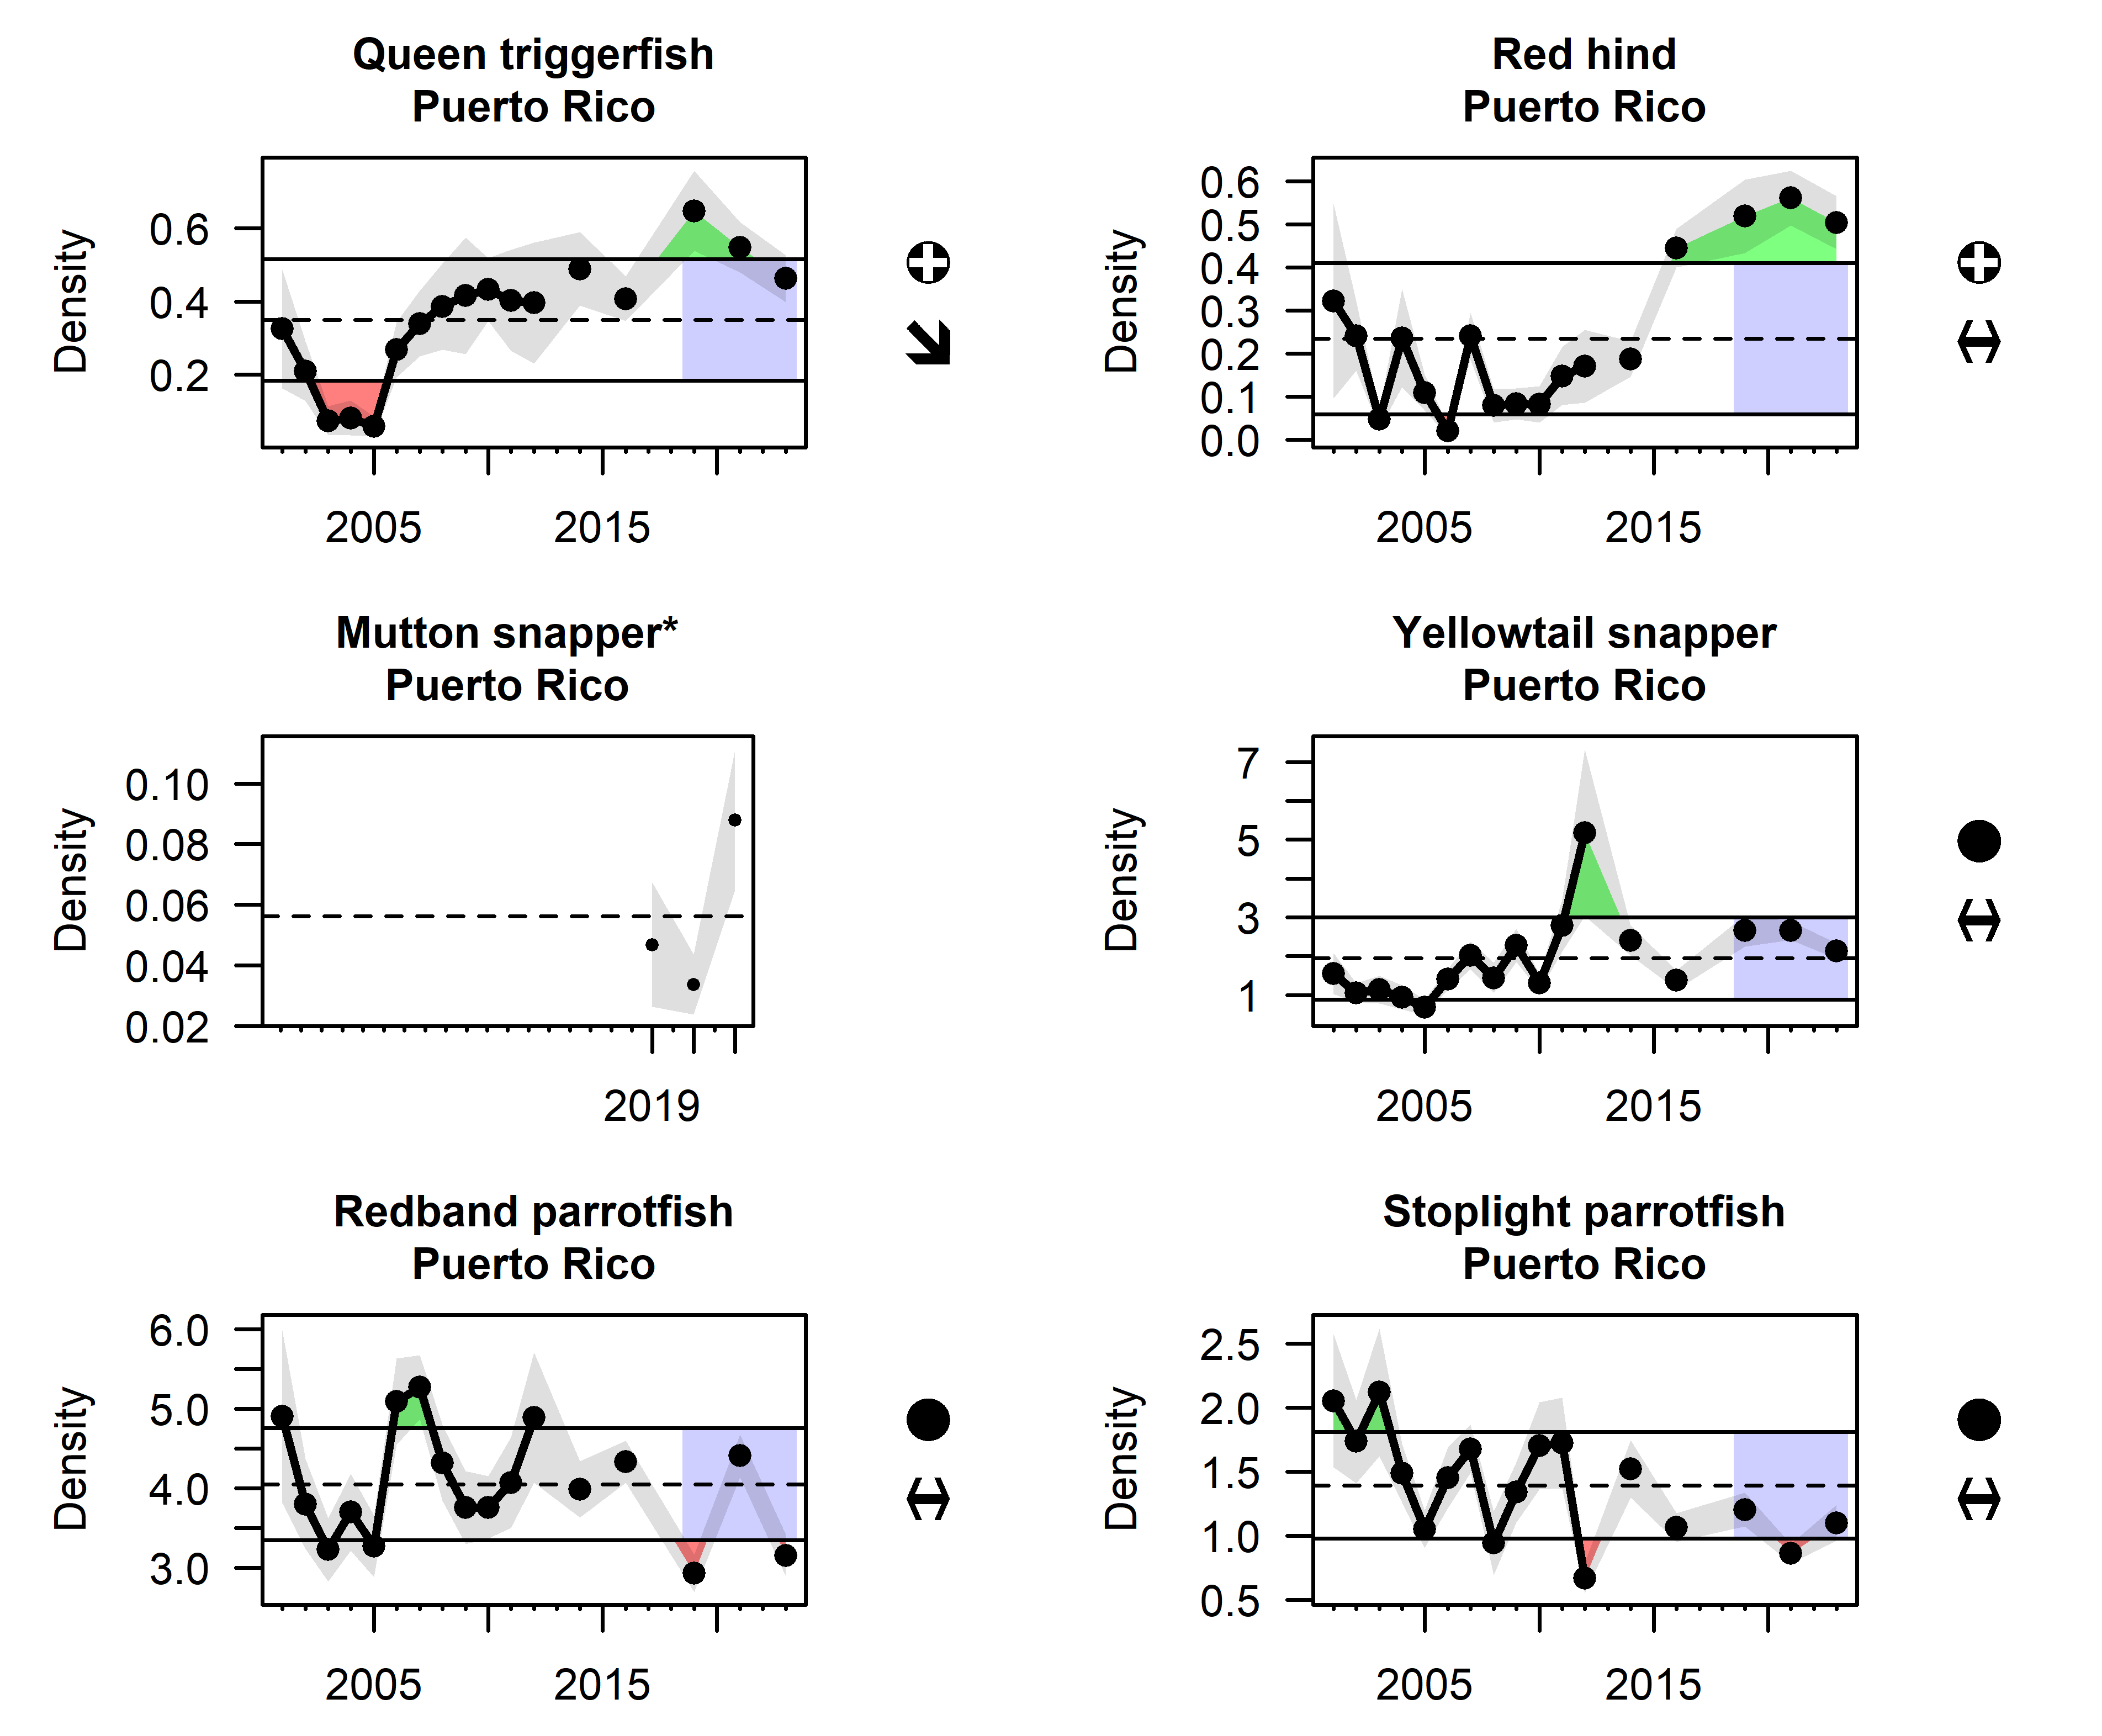
\includegraphics[width=0.9\linewidth,height=\textheight,keepaspectratio]{indicator_plots/RVC_PR_plot_final.png}

}

\caption{\label{fig-RVCPR}Average density of queen triggerfish, red
hind, lane snapper, yellowtail snapper, redband parrotfish, and
stoplight parrotfish in Puerto Rico from the National Coral Reef
Monitoring Program's Reef Visual Census data.}

\end{figure}%

\begin{figure}

\centering{

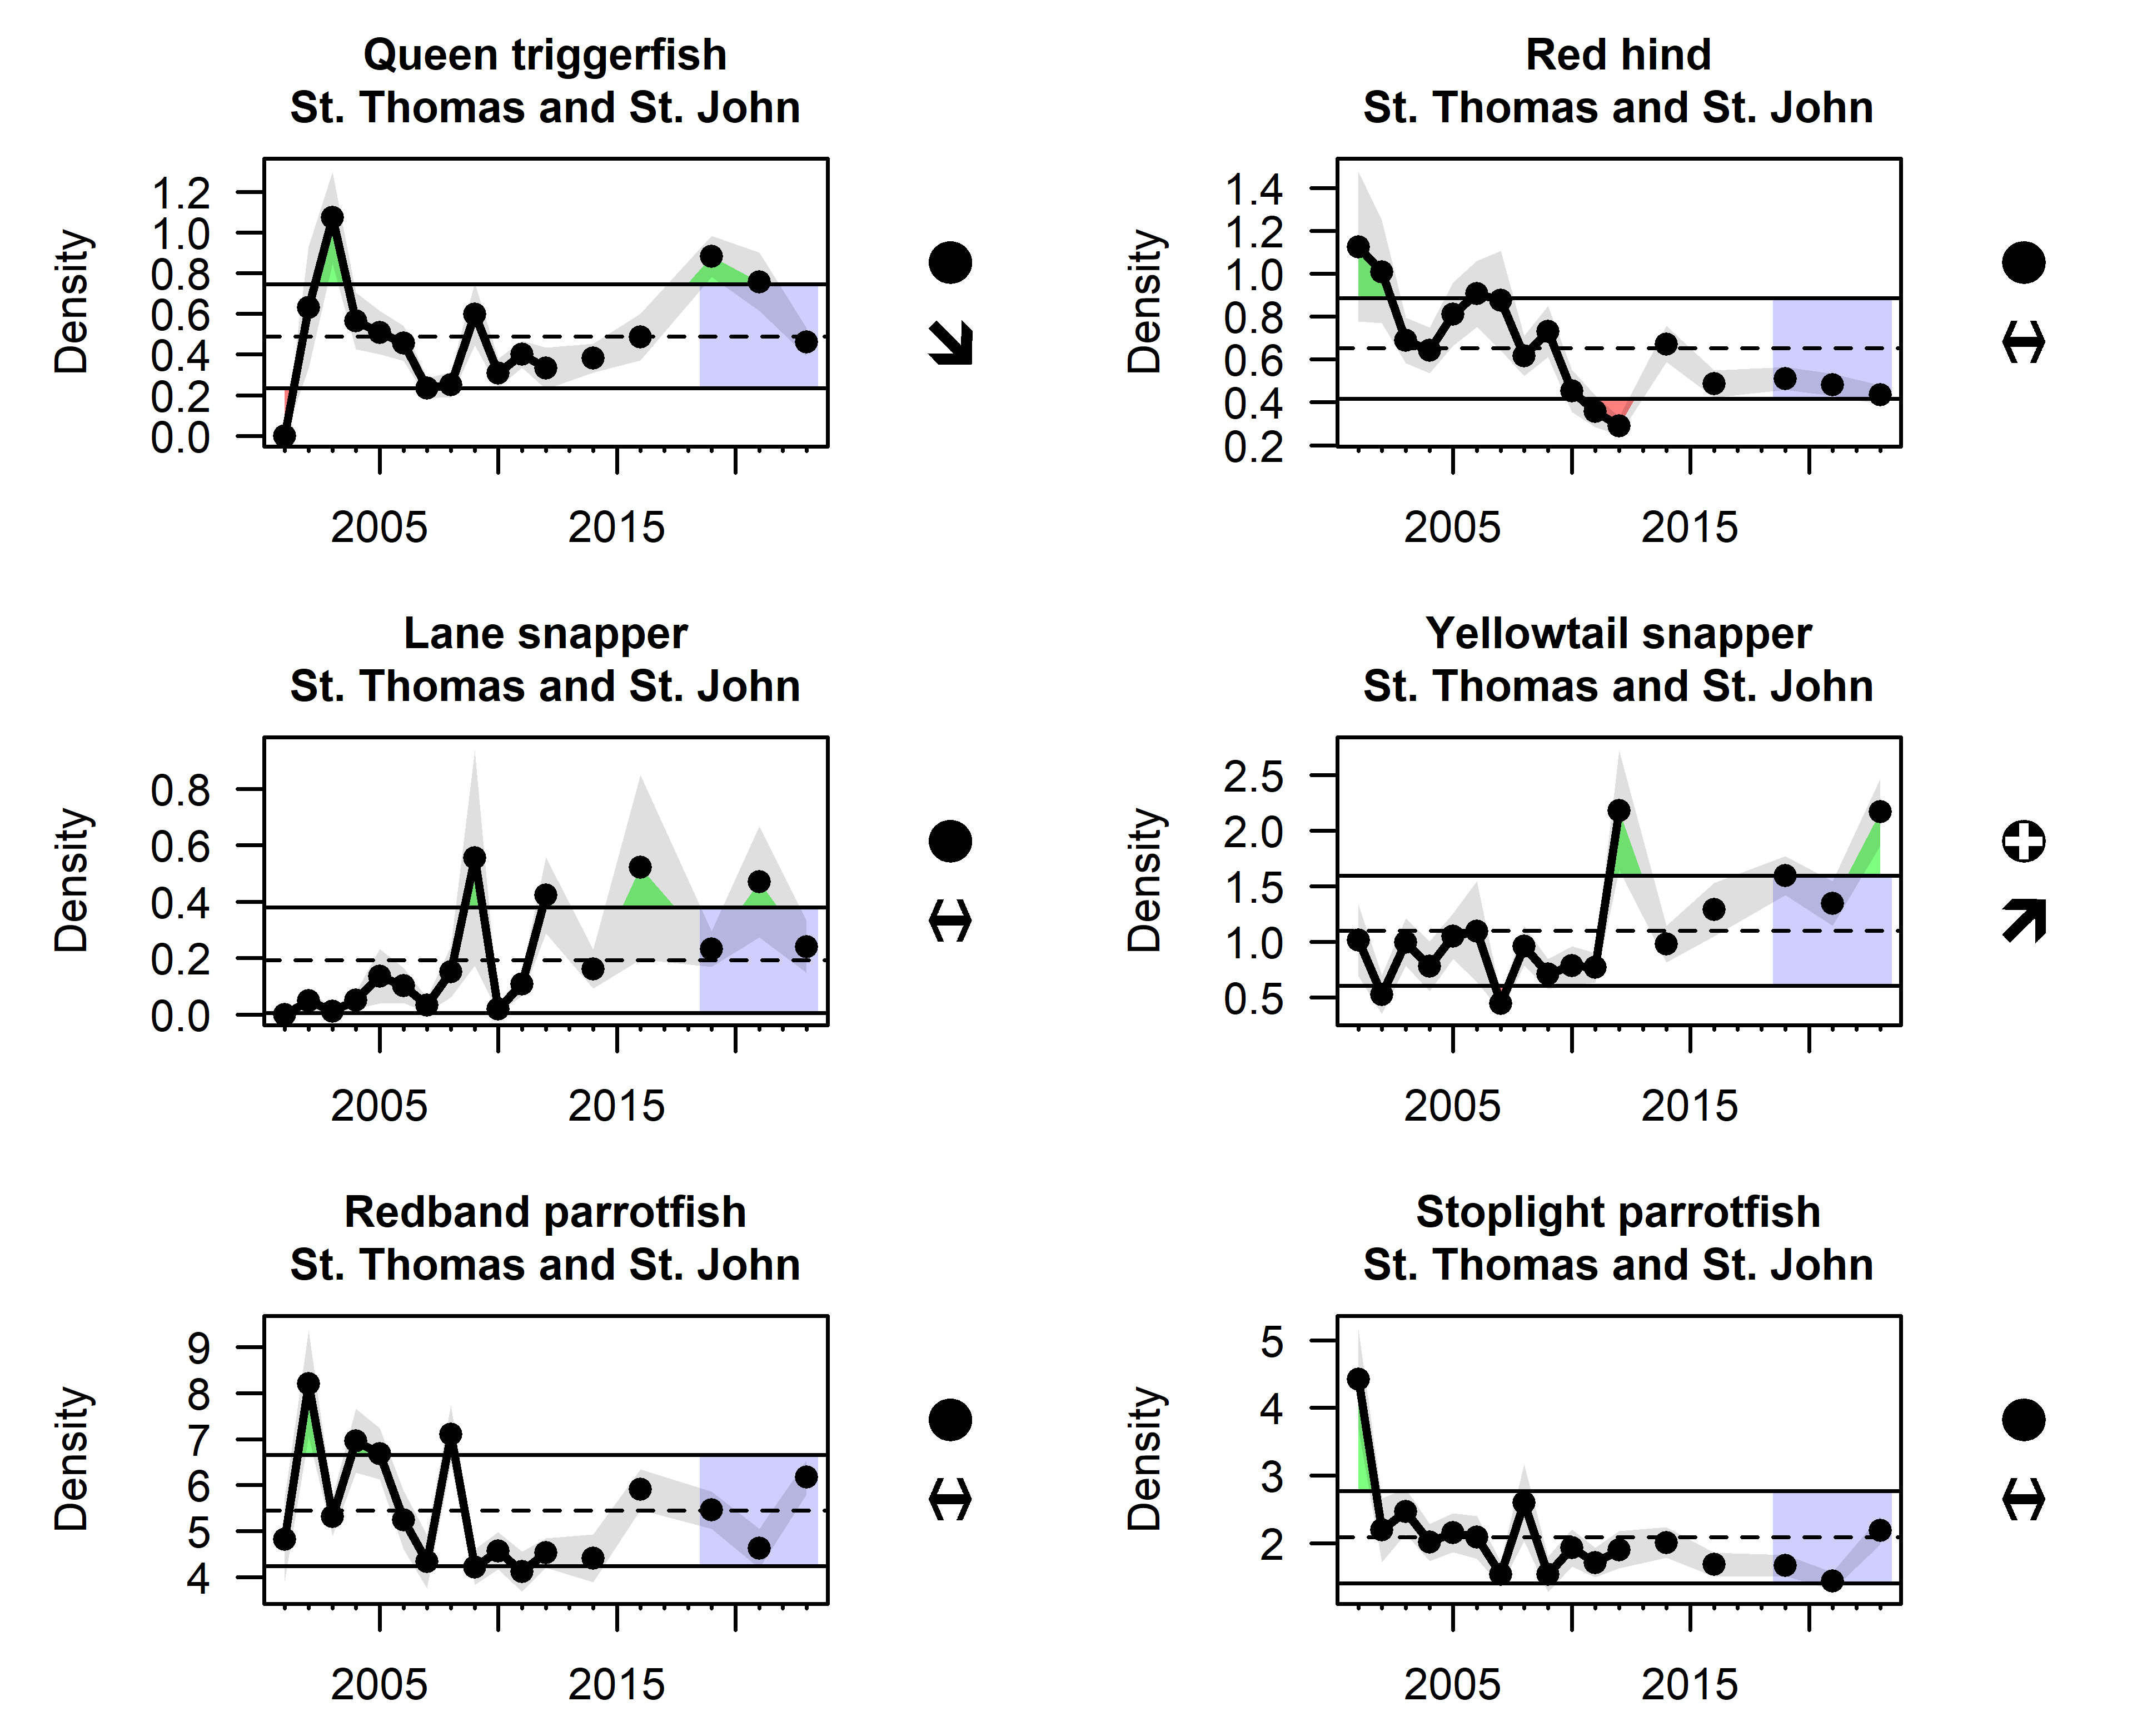
\includegraphics[width=0.9\linewidth,height=\textheight,keepaspectratio]{indicator_plots/RVC_STSJ_plot_final.png}

}

\caption{\label{fig-RVCSTSJ}Average density of queen triggerfish, red
hind, lane snapper, yellowtail snapper, redband parrotfish, and
stoplight parrotfish in St.~Thomas and St.~John from the National Coral
Reef Monitoring Program's Reef Visual Census data.}

\end{figure}%

\begin{figure}

\centering{

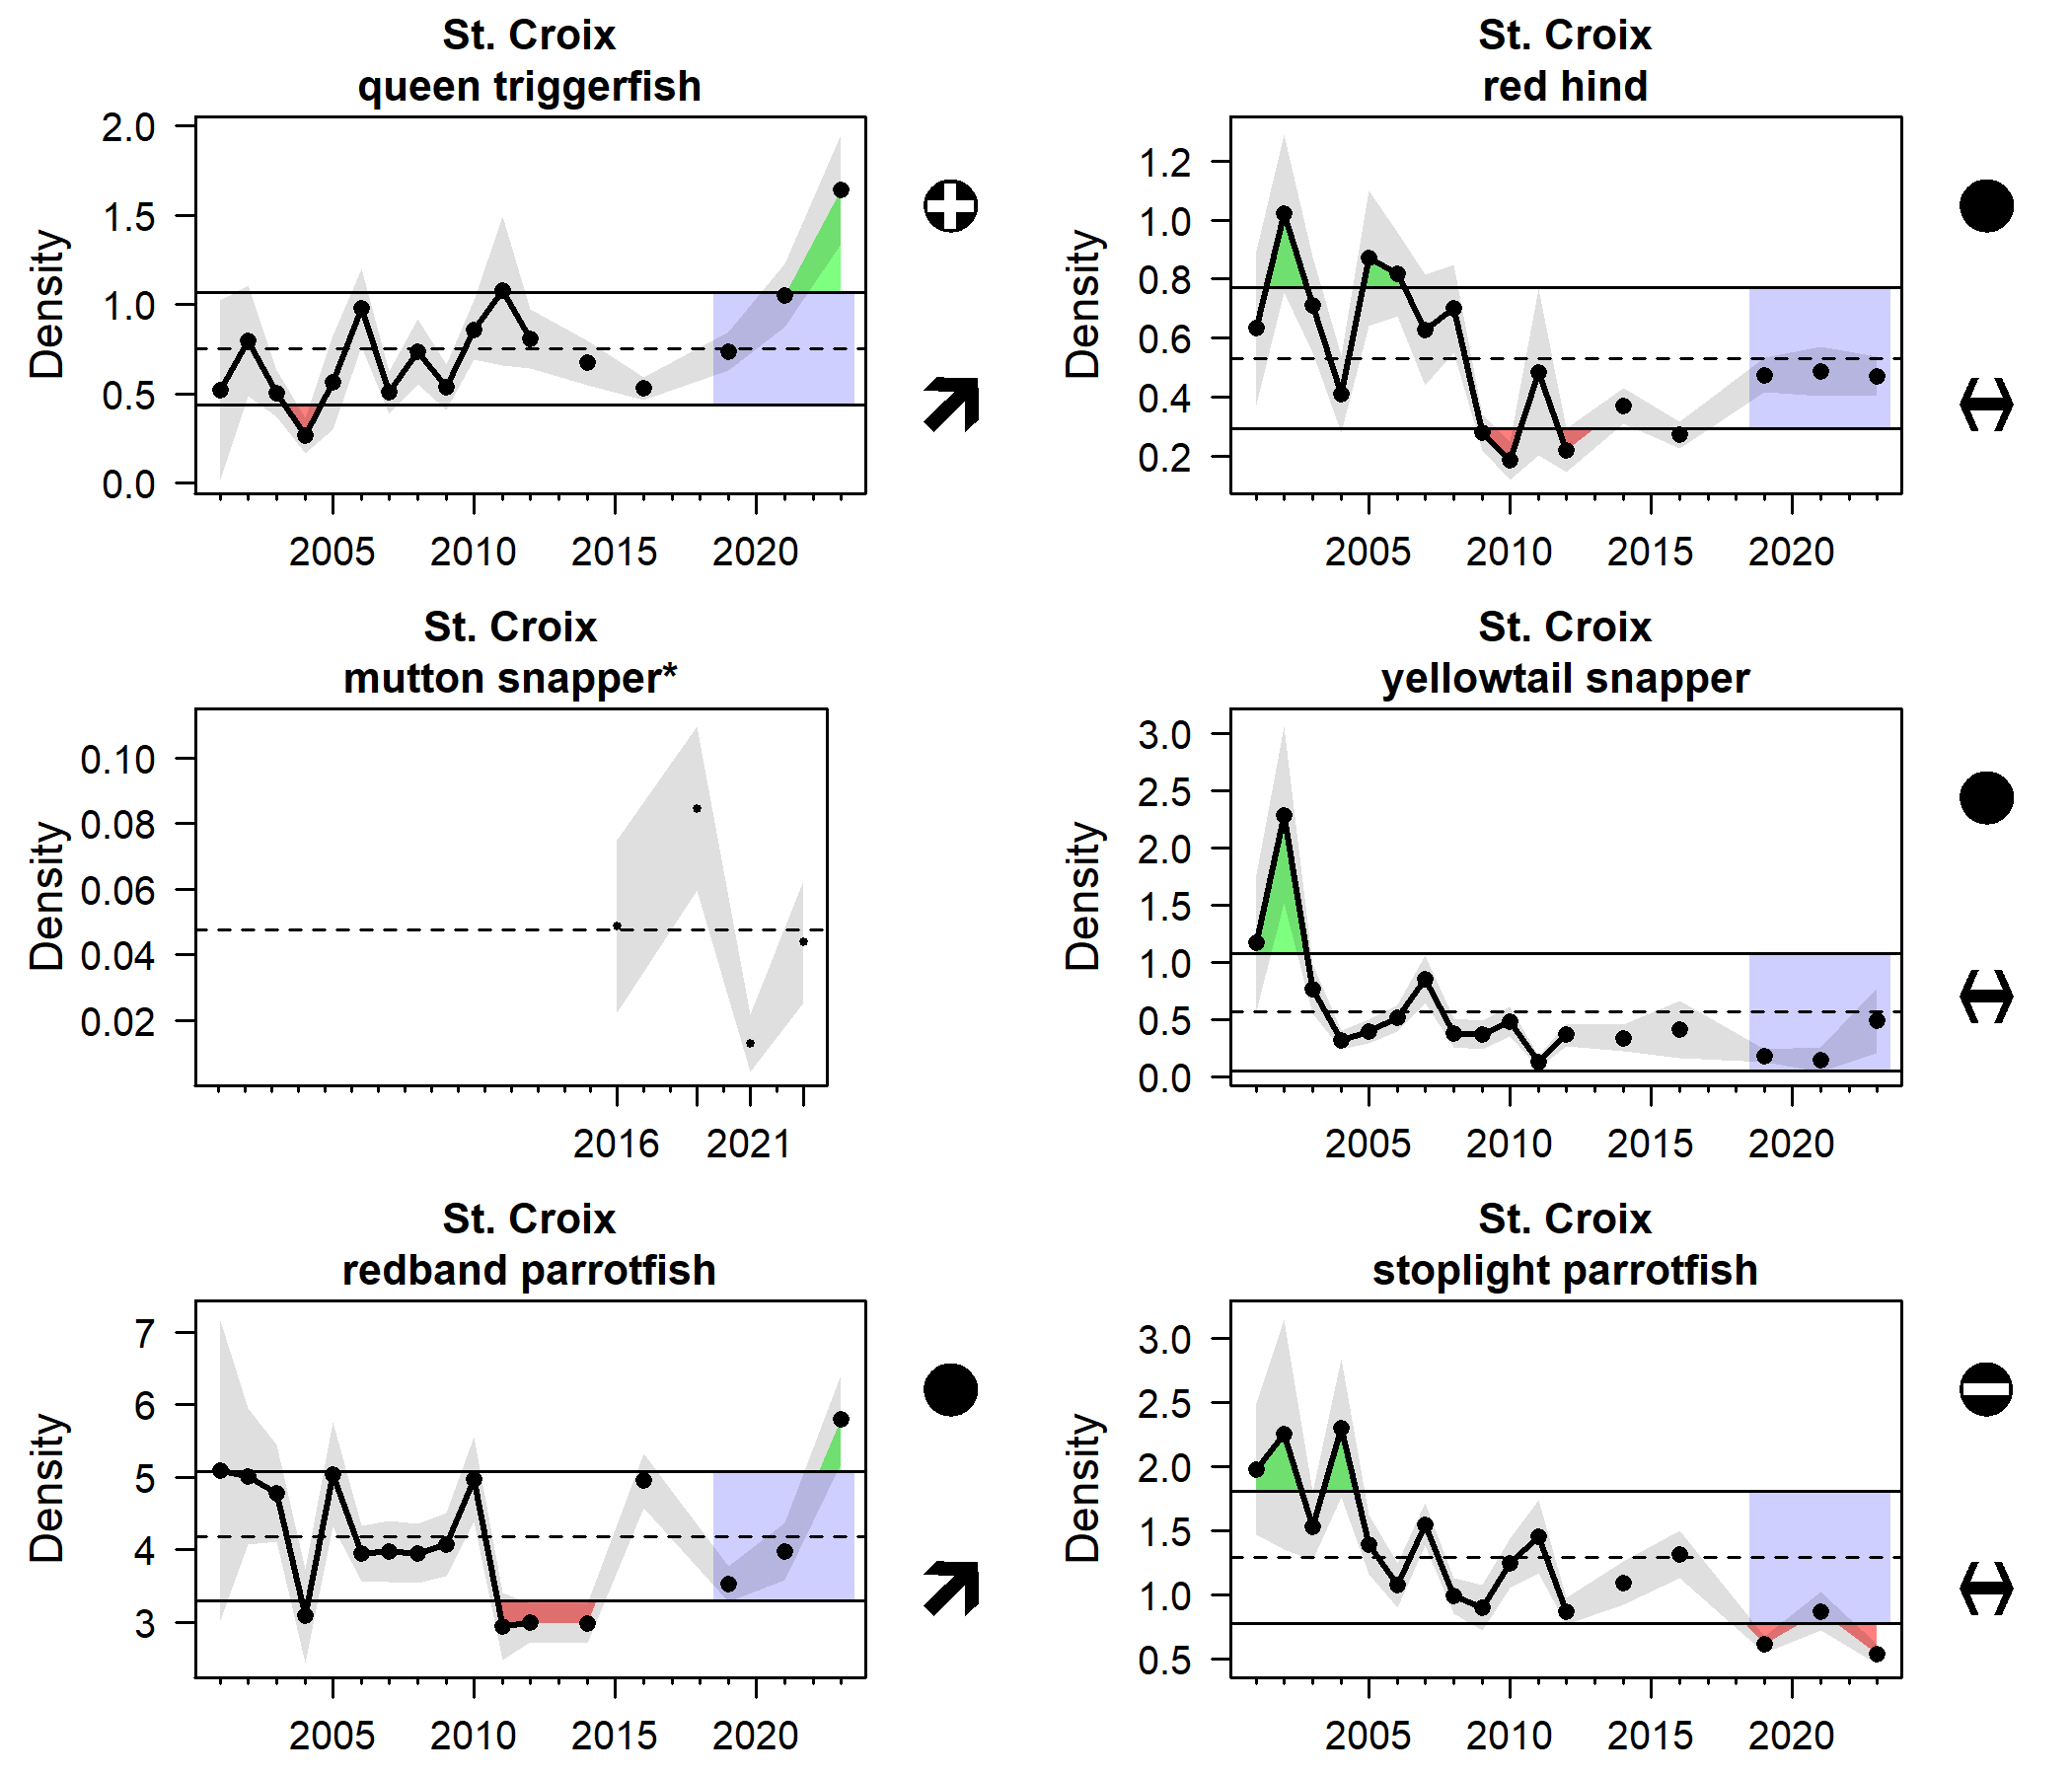
\includegraphics[width=0.9\linewidth,height=\textheight,keepaspectratio]{indicator_plots/RVC_STX_plot_final.png}

}

\caption{\label{fig-RVCSTX}Average density of queen triggerfish, red
hind, lane snapper, yellowtail snapper, redband parrotfish, and
stoplight parrotfish in St.~Croix from the National Coral Reef
Monitoring Program's Reef Visual Census data.}

\end{figure}%

Fishery-independent surveys can be used to look at changes in the
overall fish community and understand processes affecting multiple
suites of species. The Puerto Rico Long-Term Coral Reef Monitoring
Program (PRCRMP) has conducted annual surveys of fish and benthic
organisms since 1999 (Puerto Rico Department of Natural and
Environmental Resources 2019). Similarly, the USVI Territorial Coral
Reef Monitoring Program (TCRMP) conducts annual to semi-annual surveys
of coral health, fish community structure and coral health
(\href{https://www.google.com/url?q=https://www.vitcrmp.org/&sa=D&source=docs&ust=1733763590069103&usg=AOvVaw2nwqg9fhvdZ3k4tlJFQWV2}{https://www.vitcrmp.org/}).
The PRCRMP, TCRMP, and NCRMP programs are all supported by NOAA's Coral
Reef Conservation Program and are complementary, with PRCRMP and TCRMP
sampling at fixed sites and NCRMP sampling at stratified random sites.
Commercial fish density is calculated by taking the average number of
commercially targeted fish per transect over time. The slope of the size
spectrum is calculated by binning all observed commercial fish lengths
into size categories and then fitting a linear regression through the
log-transformed histogram; a more negative slope represents relatively
fewer large fish and potentially increased fishing impacts. In Puerto
Rico, average commercial fish density fluctuates but is stable over
time; insufficient data were available with which to estimate the slope
of the size spectra. In the USVI, commercial fish density has increased
since the early 2010s, with notable peaks in 2018 and 2021. The slope of
the size spectrum has been relatively stable over time but with sudden
drops in 2011 and 2018. A single-year increase in density combined with
a simultaneous decrease in the size spectrum conveys the sudden
appearance of many small fish, suggestive of a large recruitment event
across multiple species in 2018 (Figure~\ref{fig-fishdensity}).

\begin{figure}

\centering{

\pandocbounded{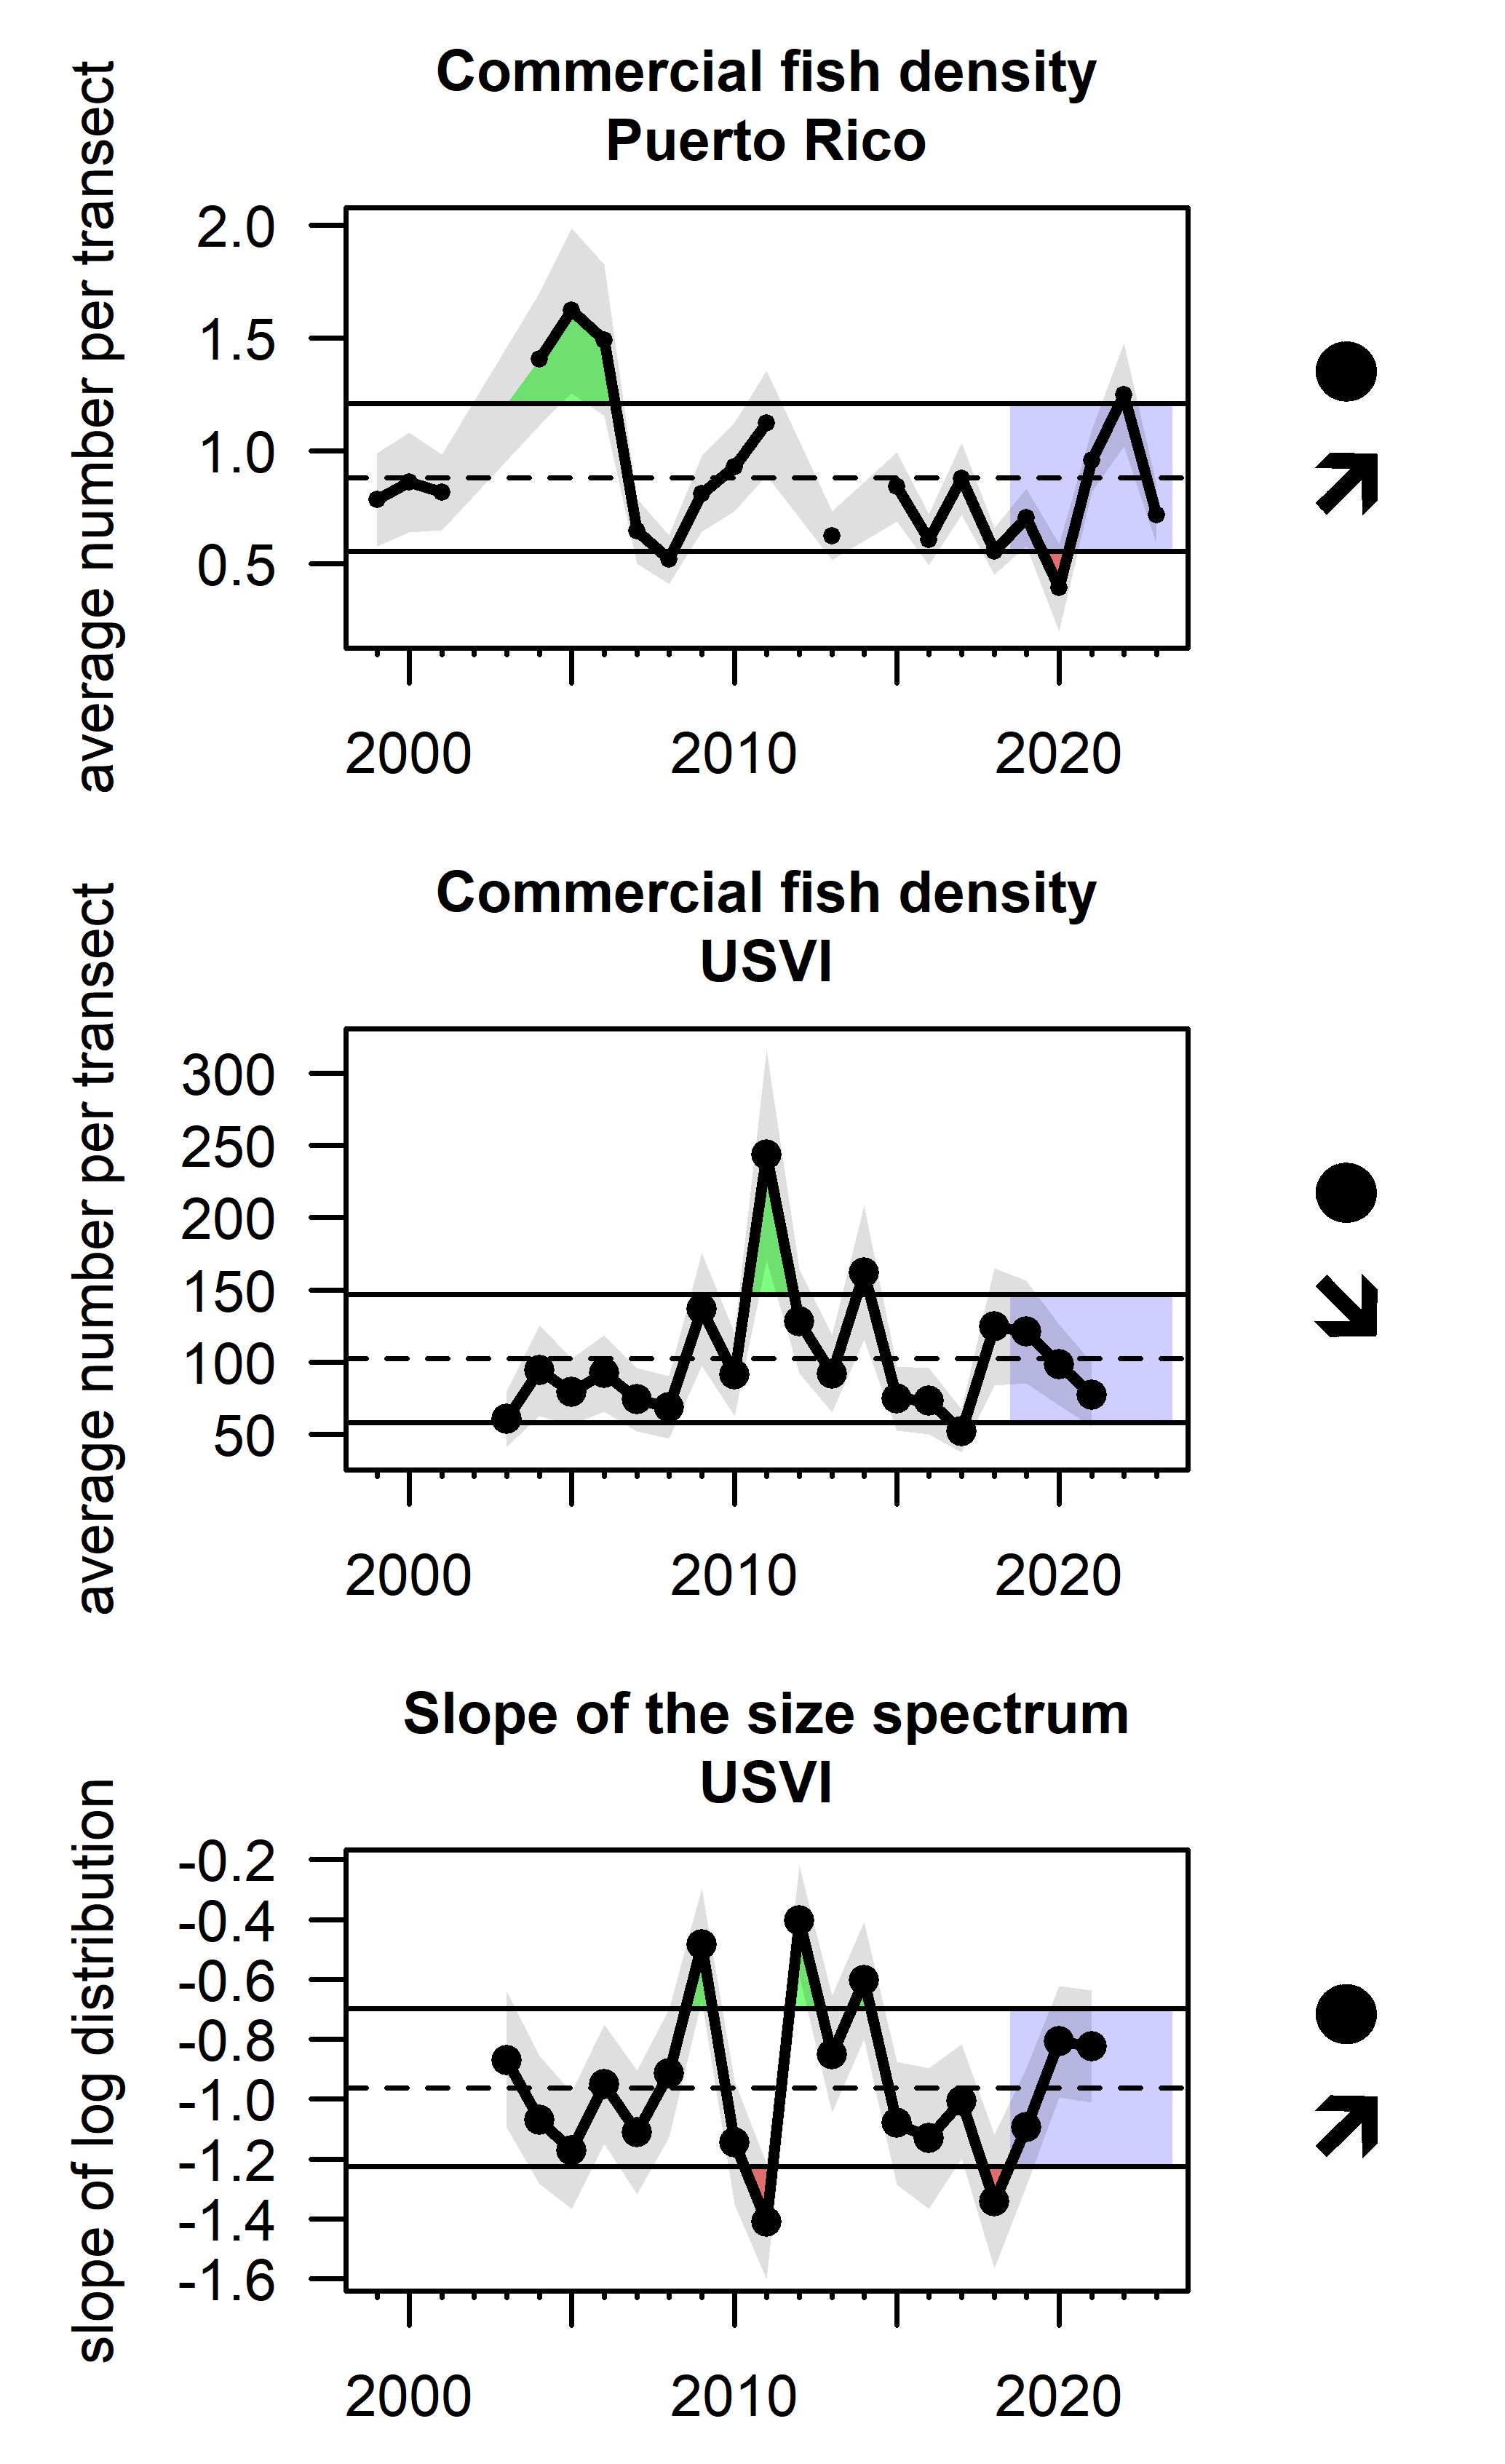
\includegraphics[keepaspectratio]{indicator_plots/fish_density_plot_final.png}}

}

\caption{\label{fig-fishdensity}Commercial fish density from PRCRMP
fishery-independent surveys in Puerto Rico (top), commercial fish
density from TCRMP fishery-independent surveys in the USVI (middle), and
the slope of the log-transformed size spectrum from TCRMP surveys in the
USVI (bottom).}

\end{figure}%

\subsection{Pelagic:demersal ratio of
landings}\label{pelagicdemersal-ratio-of-landings}

The ratio of pelagic to demersal species is thought to be responsive to
nutrient inputs and the quality of benthic habitat in marine ecosystems
(de Leiva Moreno et al. 2000); in the context of small islands in the
tropical seas, it may convey the availability and productivity of
pelagic habitats relative to the size of the shelf and productivity of
coral reef habitats. Ratios of pelagic to demersal landings were
calculated based on total pounds reported in the Caribbean Commercial
Landings data, following a classification of all species based on their
reported ecology in FishBase (Froese and Pauly 2024). In St.~Croix, the
pelagic-demersal ratio is much higher than the other islands, due to the
small shelf area and limited availability of reef habitat; interannual
fluctuations for this island are largely influenced by landings of
dolphinfish and tunas. In Puerto Rico, the pelagic-demersal ratio has
increased in recent years; this may be partially due to changes in
reporting that occurred in 2020 (addition of electronic reporting
option). In St.~Thomas and St.~John, the ratio has gradually increased
over time; the large peak in the 2018--2019 fishing year could have been
a result of hurricane-induced reef habitat loss and subsequent reduction
in landings of demersal fish species (Figure~\ref{fig-PD}).

\begin{figure}

\centering{

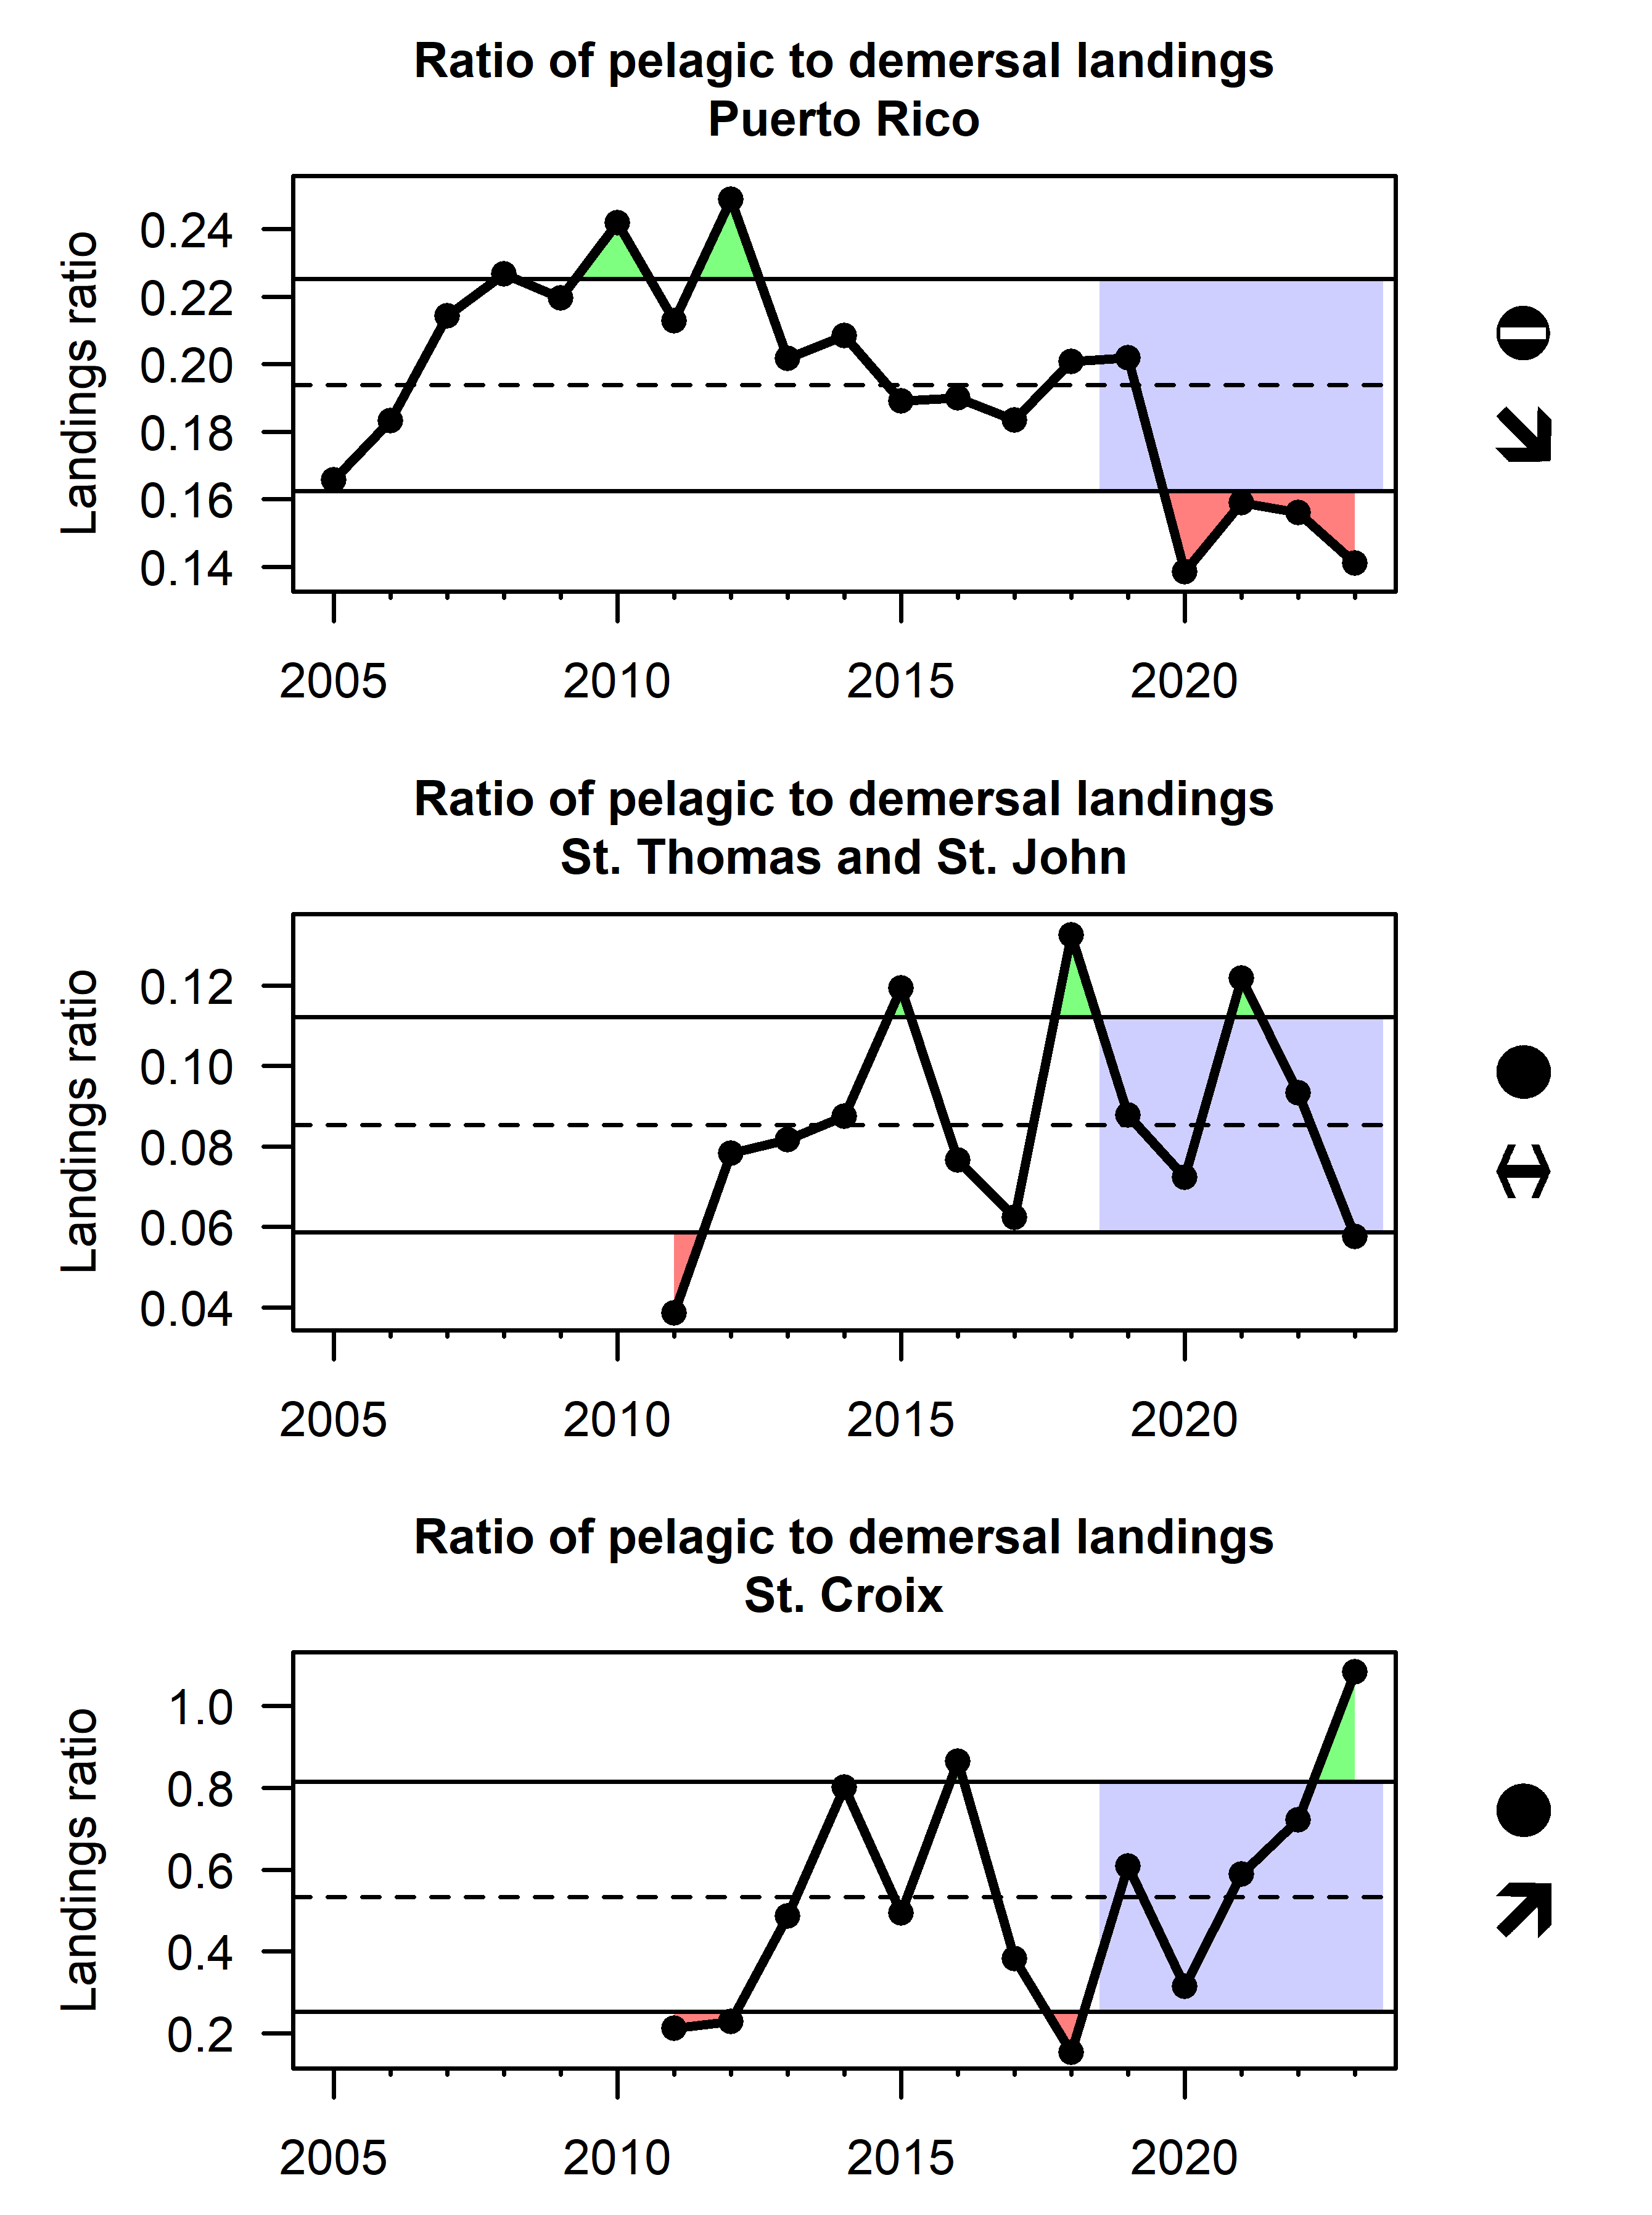
\includegraphics[width=0.6\linewidth,height=\textheight,keepaspectratio]{indicator_plots/PD_ratio_plot_final.png}

}

\caption{\label{fig-PD}Ratios of pelagic to demersal landings, based on
reported commercial landings data for Puerto Rico (top), St.~Thomas and
St.~John (middle) and St.~Croix (bottom). Note differences in scale of
the y-axes; years in the USVI are fishing years (July 1st to June 30th
of the following year).}

\end{figure}%

\subsection{Maximum length in the
landings}\label{maximum-length-in-the-landings}

The average maximum length (Lmax) of a species in the landings has been
proposed as an indicator of whether large-bodies species have been
depleted and are no longer fished (Rochet and Trenkel 2003). The Lmax
indicator is derived by assigning a maximum body length for each species
(as reported in FishBase) and then calculating the average body length
for the landings in each year (based on the Caribbean Commercial
Landings database). This analysis was limited to demersal species only,
as pelagic species tend to be larger-bodied and the index would
otherwise be highly correlated with the pelagic-demersal ratio. The
average maximum length in the demersal landings decreased over time in
Puerto Rico from 2005--2012, but has been relatively stable since
(Figure~\ref{fig-avgLmax}). In the USVI, there has been no overall trend
over time, though there was a sharp decline in St.~Thomas and St.~John
in the 2017--2018 fishing year and a sharp increase in St.~Croix in the
2018--2019 fishing year. These changes may reflect changes in fishing
behavior tied to impacts from the 2017 hurricanes.

\begin{figure}

\centering{

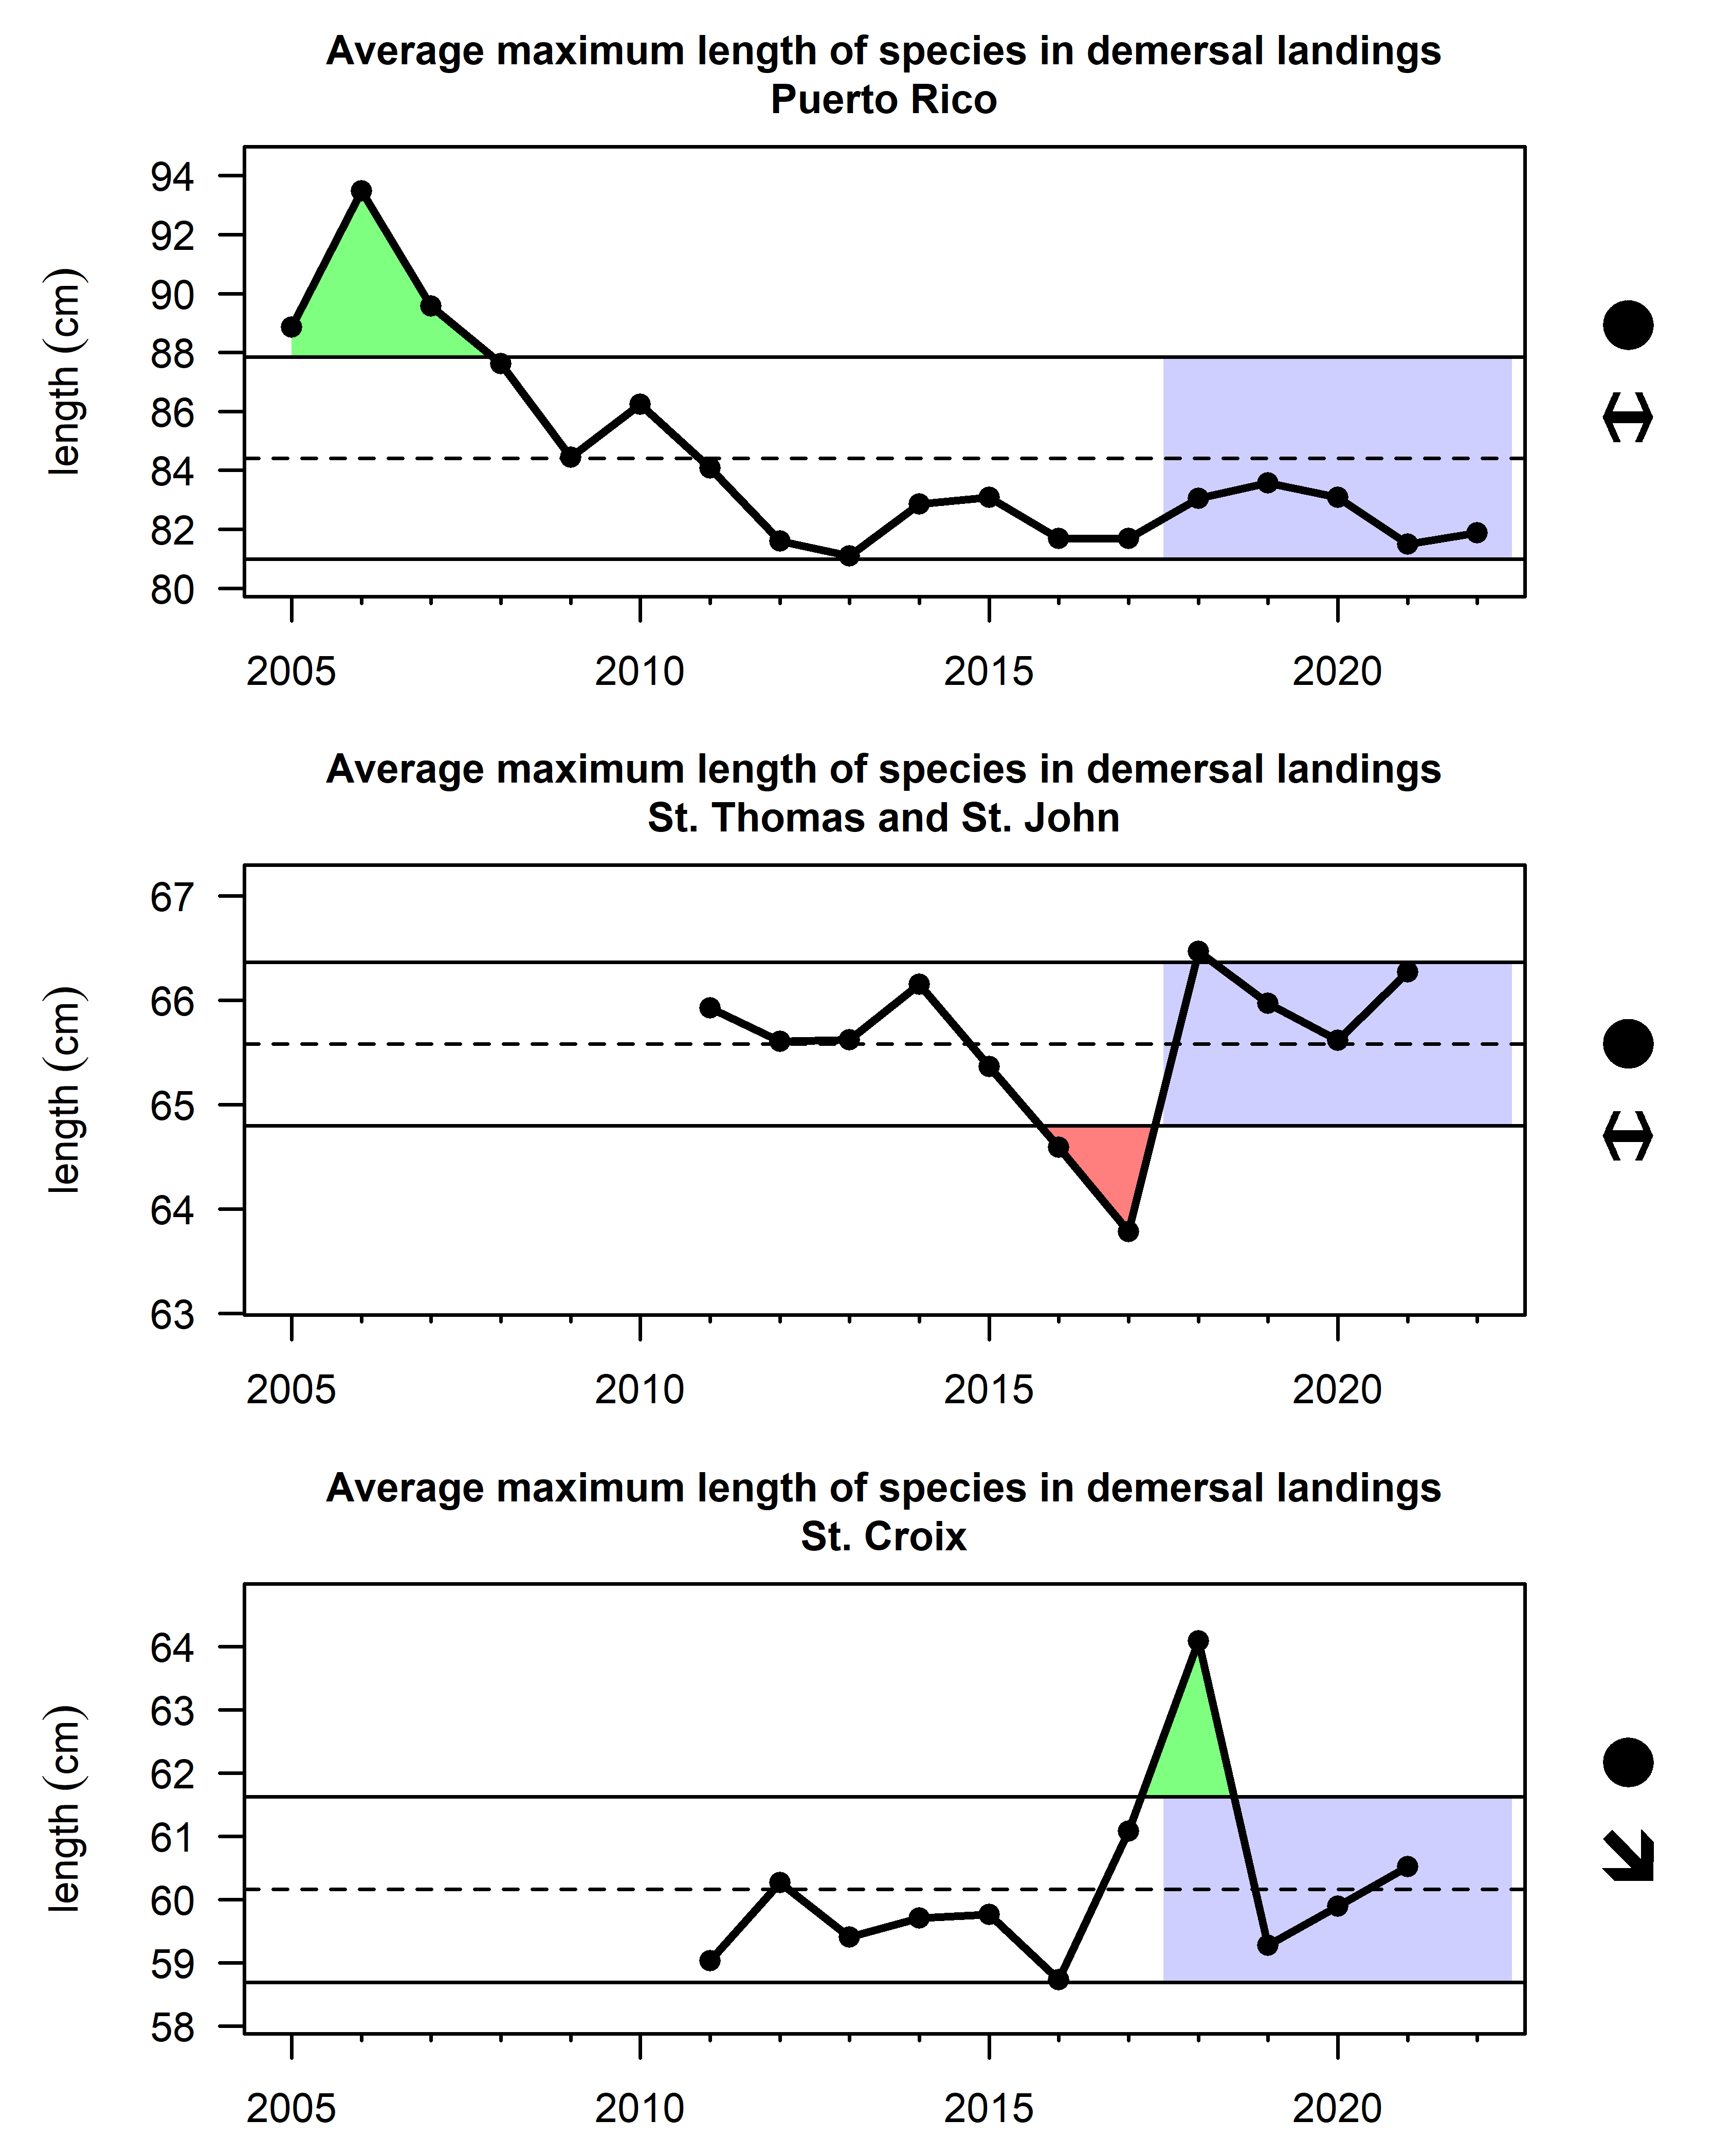
\includegraphics[width=0.6\linewidth,height=\textheight,keepaspectratio]{indicator_plots/avgLmax_plot_final.png}

}

\caption{\label{fig-avgLmax}Average maximum length of demersal species
in the reported landings for Puerto Rico (top), St.~Thomas and St.~John
(middle) and St.~Croix (bottom). Note that the years in the USVI are
fishing years (July 1st to June 30th of the following year).}

\end{figure}%

The proportion of landings within different Lmax classes can also be
shown to better understand changes driving the average Lmax value. In
Puerto Rico, there is a generally increasing trend of ``plate-sized''
fish in the 60-100cm category which is driven by increased landings of
deepwater snapper species and yellowtail snapper, while a decrease in
the 100-200cm Lmax group is driven by declining landings of large-bodies
parrotfishes, snook, and some large groupers (Figure~\ref{fig-PRLmax}).
Recent decreases in the 40-60cm Lmax group are driven by landings of
lane snapper and queen triggerfish.

\begin{figure}

\centering{

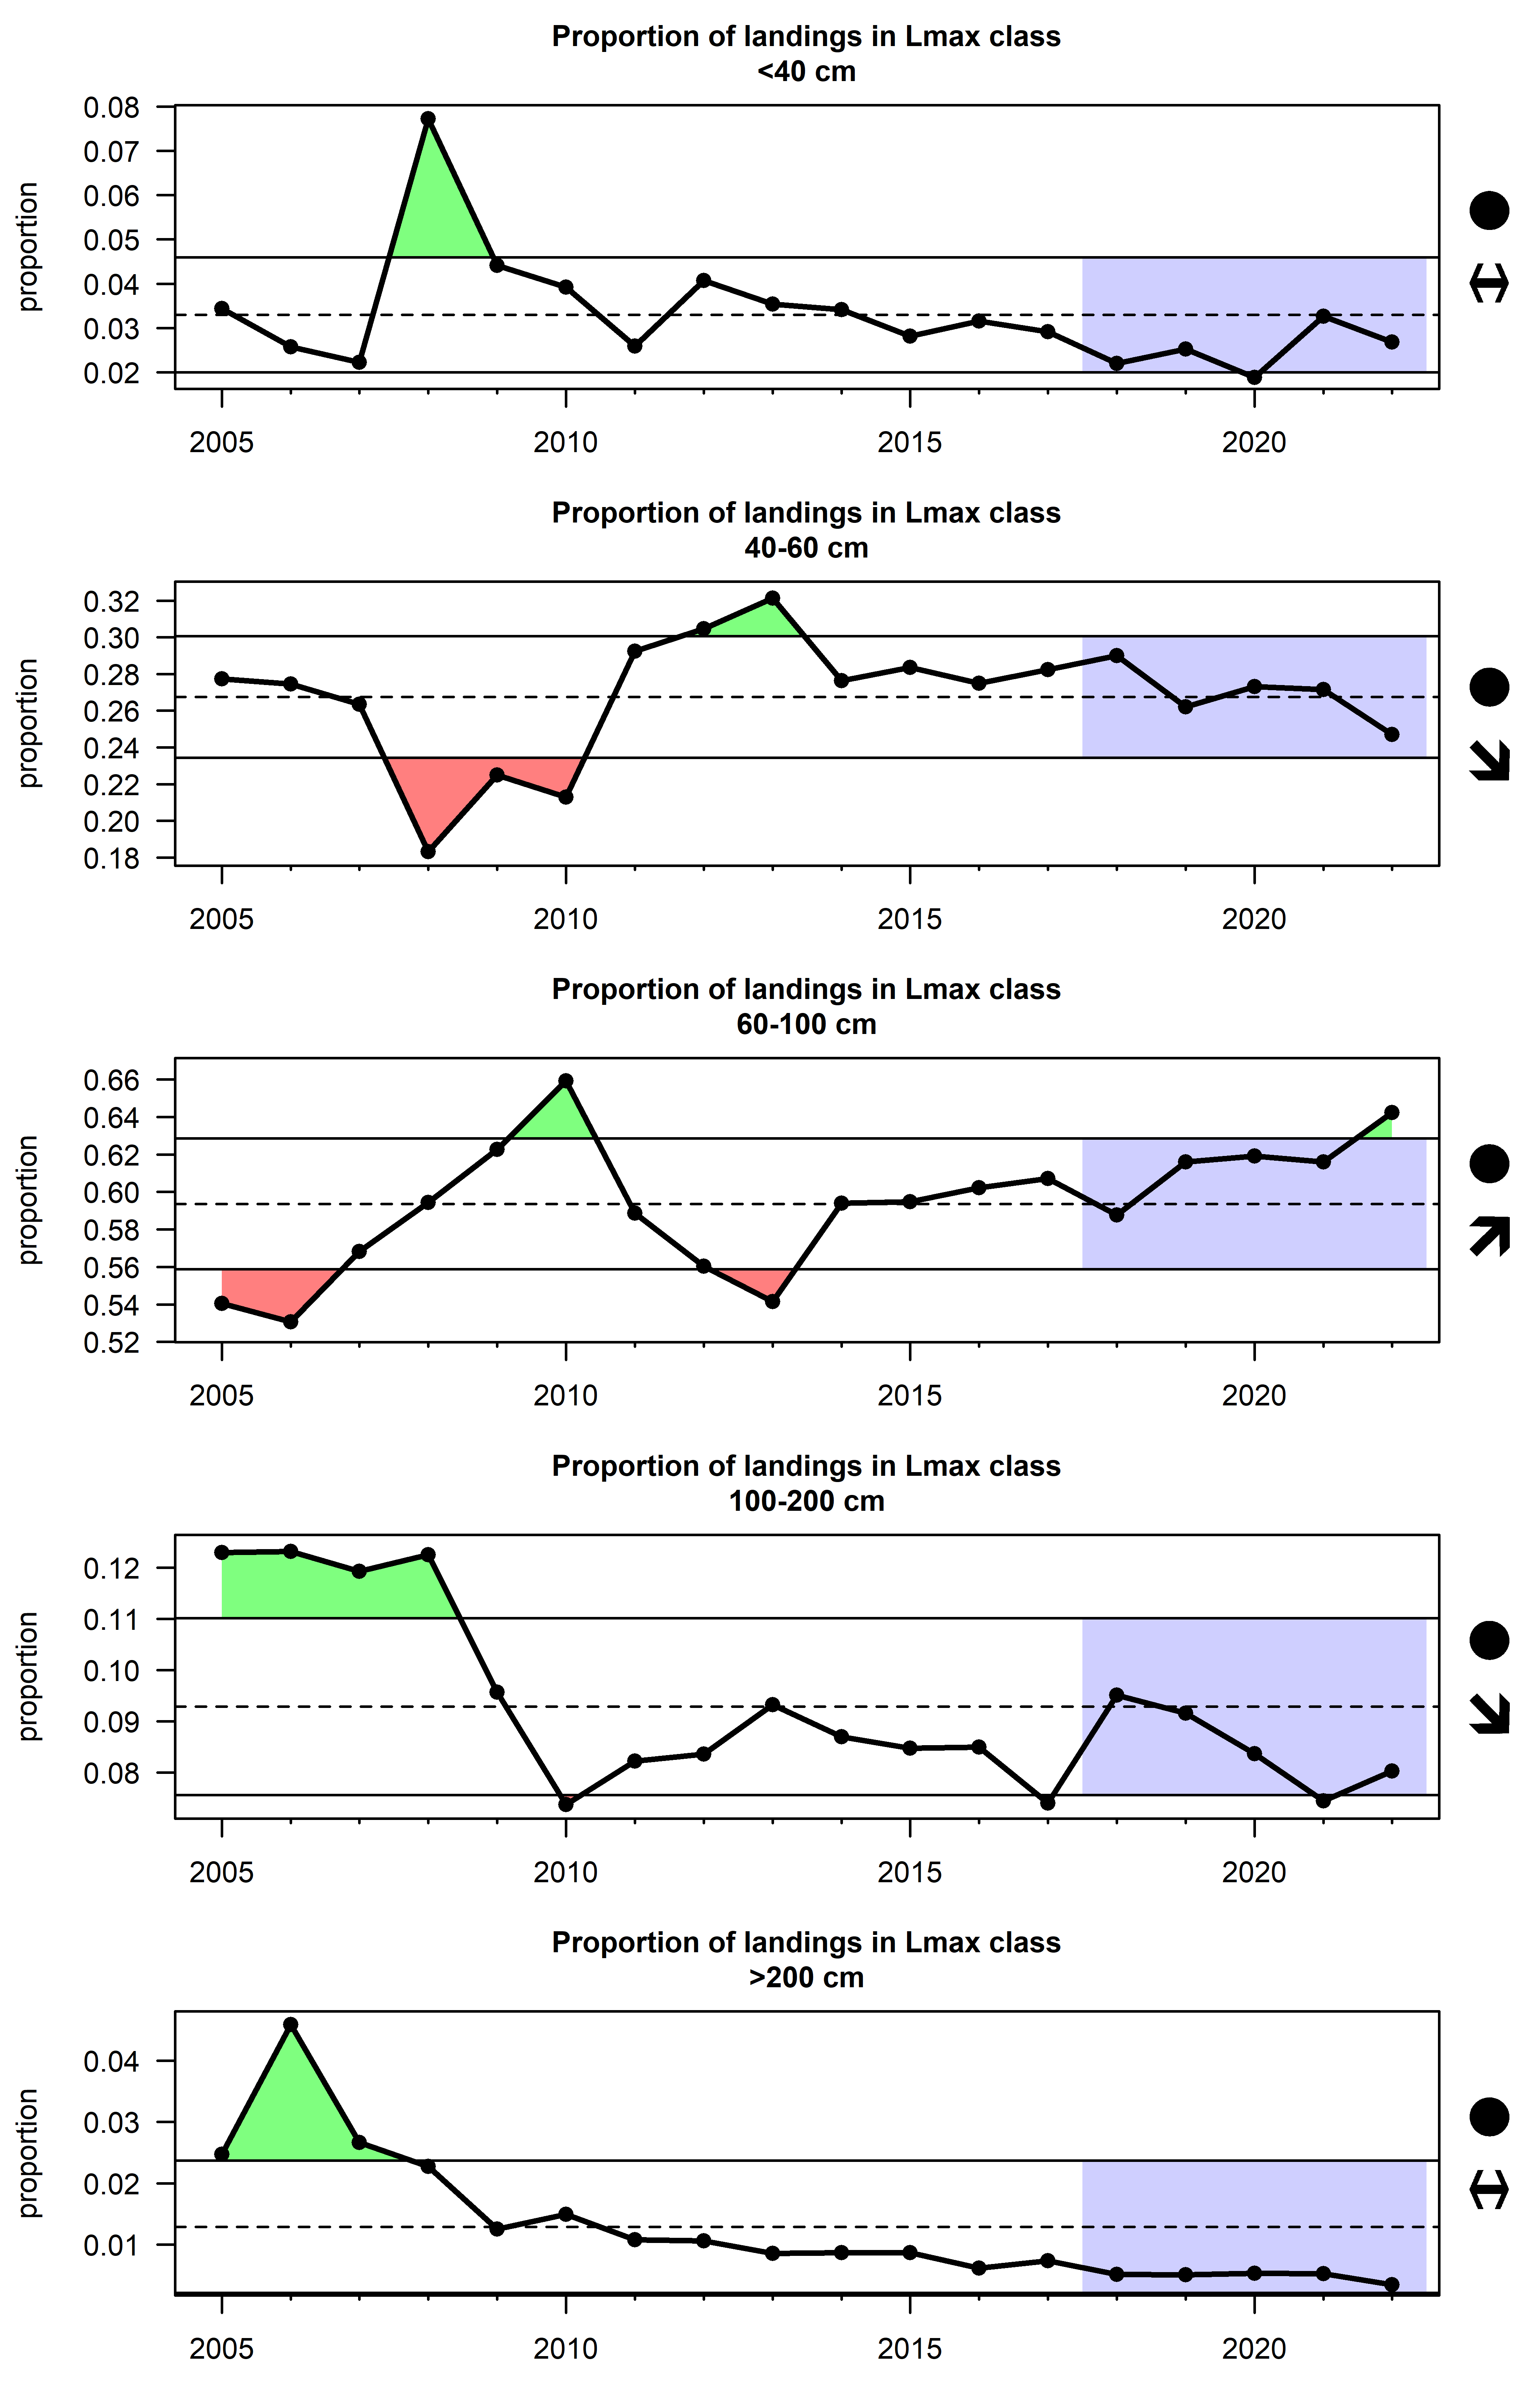
\includegraphics[width=0.6\linewidth,height=\textheight,keepaspectratio]{indicator_plots/PR_Lmax_classes_plot_final.png}

}

\caption{\label{fig-PRLmax}Proportion of commercial demersal landings in
each of four maximum body length size classes in Puerto Rico.}

\end{figure}%

In St.~Thomas there is a notable decrease in the smallest size class
(dominated by landings of surgeonfishes and longspine squirrelfish) as
well as a recent decrease in the 40-60cm Lmax group, driven by landings
of queen triggerfish, gray angelfish, and white grunt. Landings in the
60-100cm Lmax group have fluctuated over time and are influenced by
landings of red hind, yellowtail snapper and blue runner
(Figure~\ref{fig-STTLmax}).

\begin{figure}

\centering{

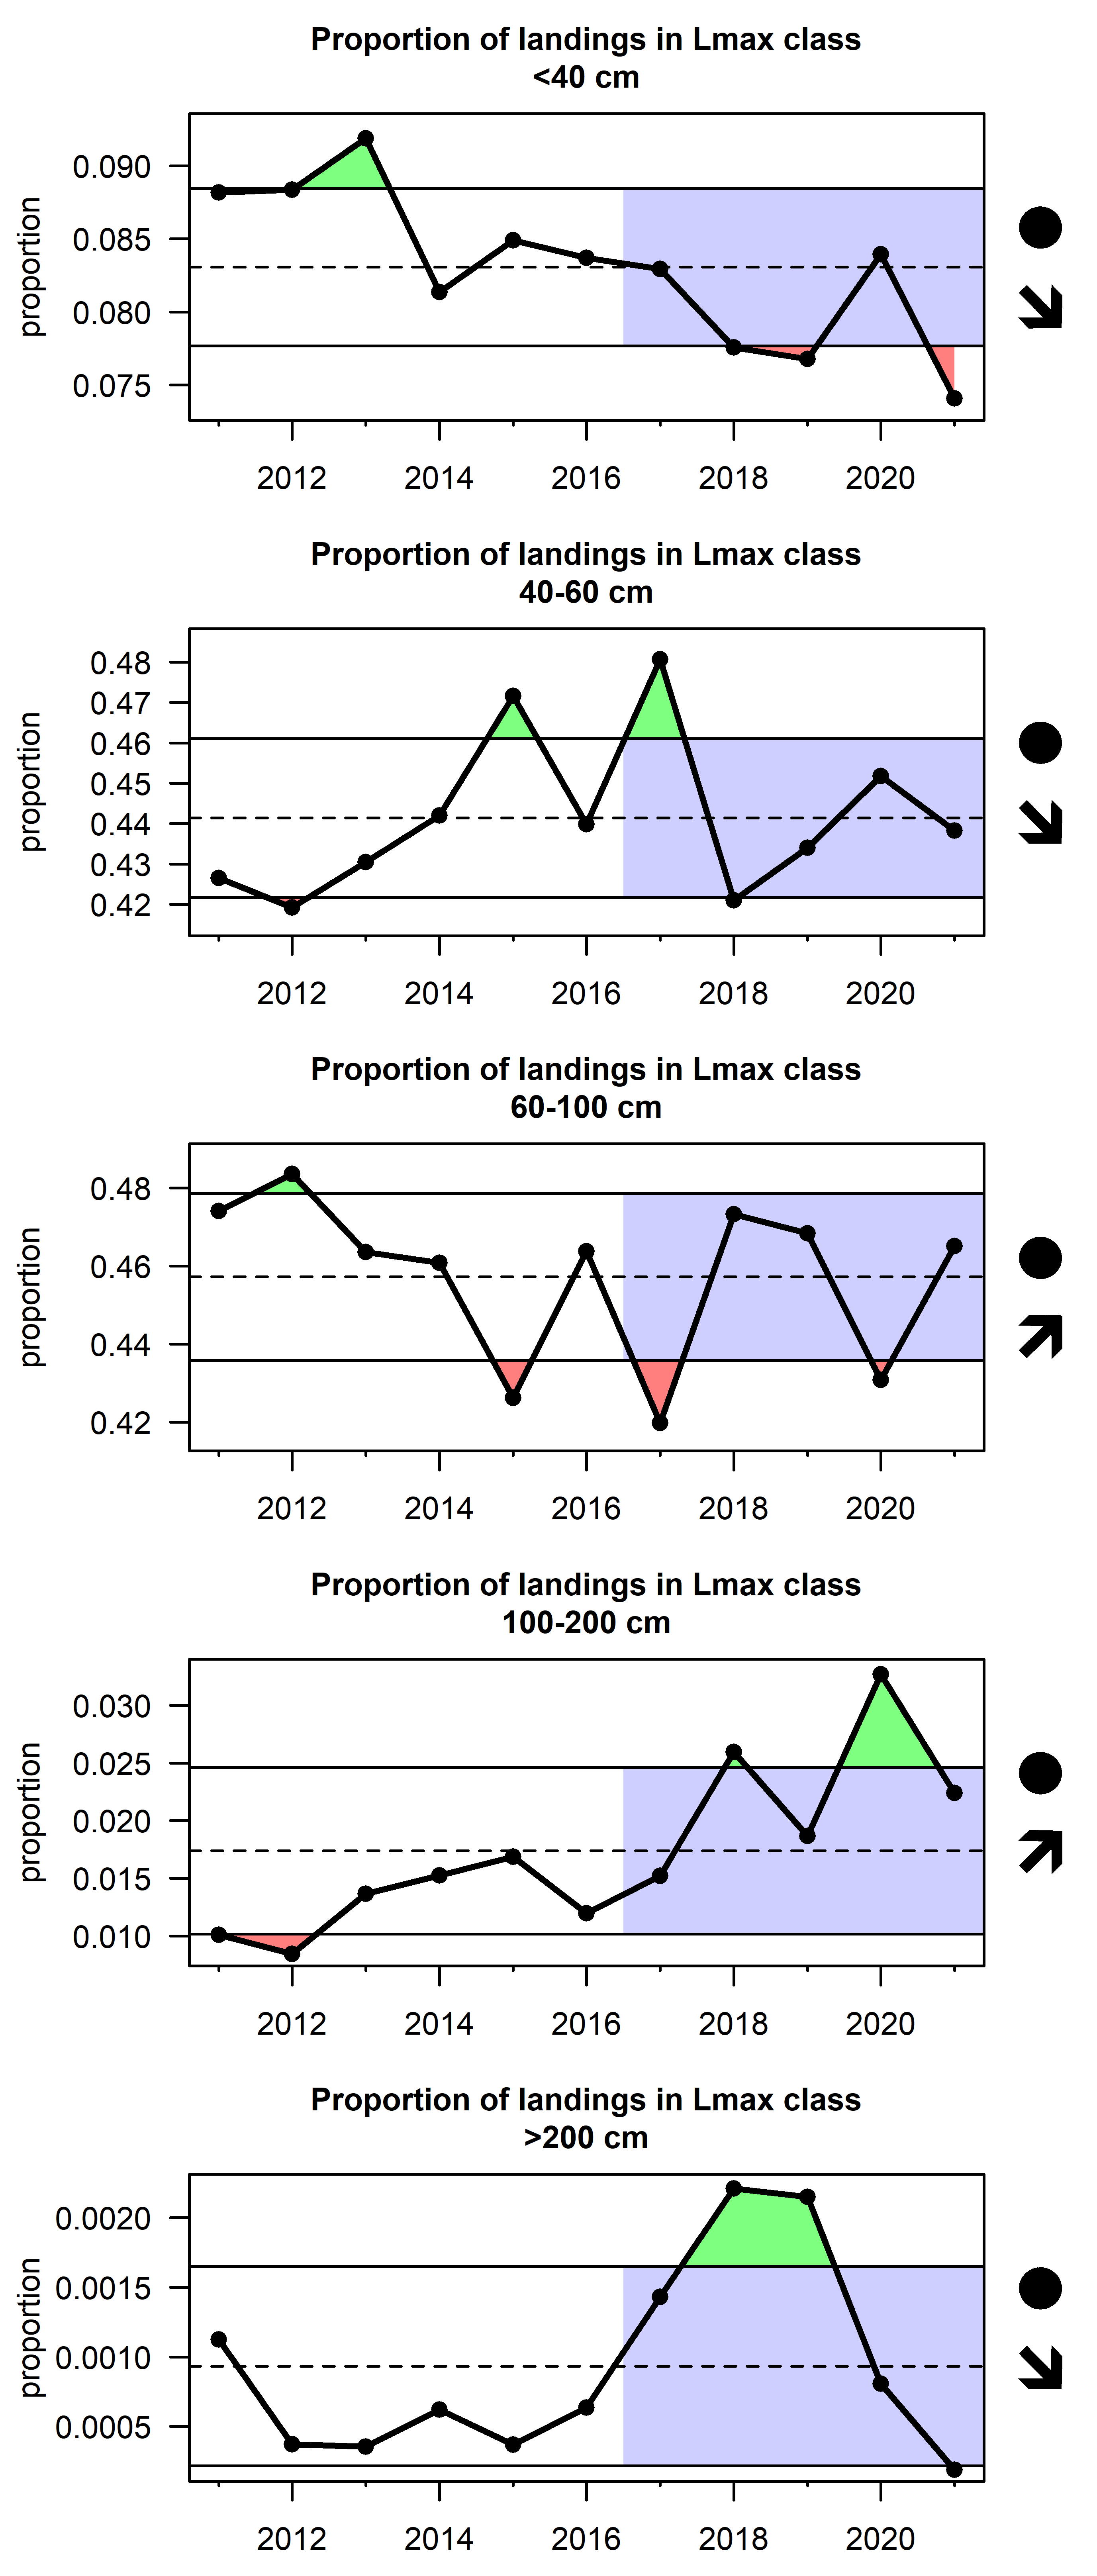
\includegraphics[width=0.6\linewidth,height=\textheight,keepaspectratio]{indicator_plots/STT_Lmax_classes_plot_final.png}

}

\caption{\label{fig-STTLmax}Proportion of commercial demersal landings
in each of four maximum body length size classes in St.~Thomas and
St.~John. Note that the years are fishing years (July 1st to June 30th
of the following year).}

\end{figure}%

In St.~Croix, changes in the maximum body size of demersal species
landings is being influenced primarily by changes in the targeting of
parrotfishes. The \textless40cm Lmax group includes redband parrotfish
and princess parrotfish and has increased in recent years, while the
40-60cm Lmax class, composed of redfin and redtail parrotfish, has
decreased in recent years. The 60-100cm Lmax class has fluctuated over
time and is driven by landings of stoplight and queen parrotfish
(Figure~\ref{fig-STXLmax}).

\begin{figure}

\centering{

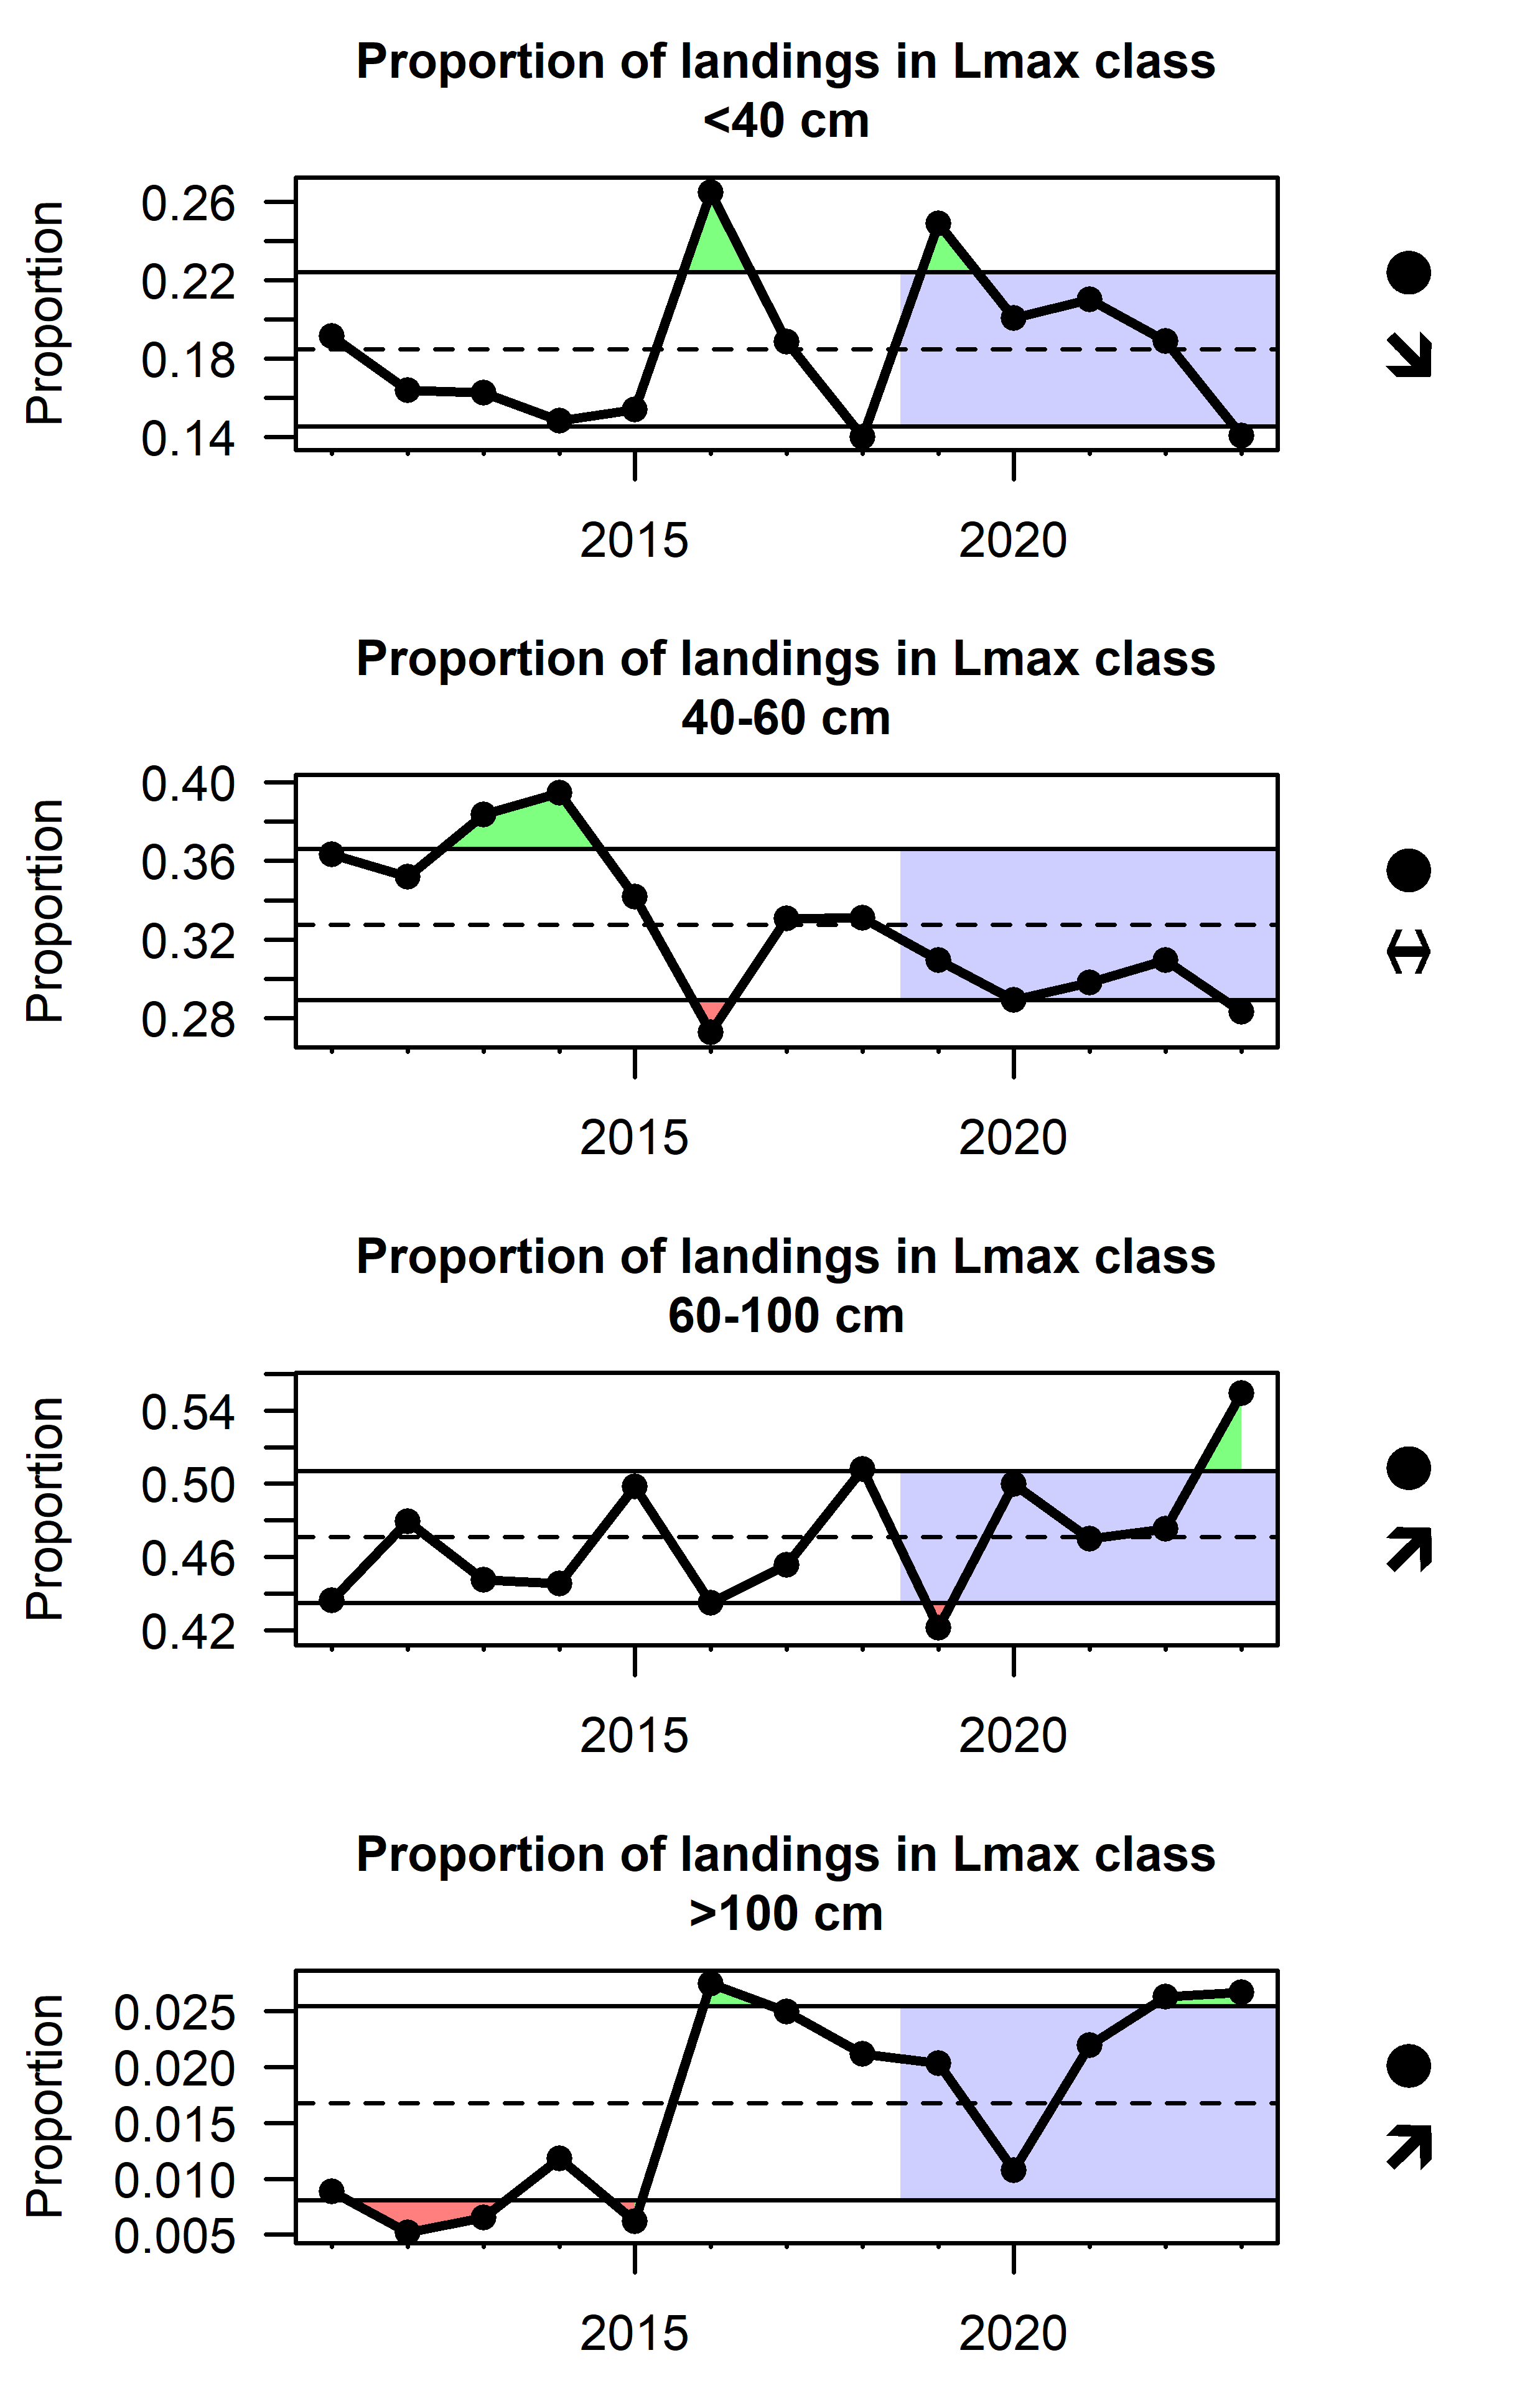
\includegraphics[width=0.6\linewidth,height=\textheight,keepaspectratio]{indicator_plots/STX_Lmax_classes_plot_final.png}

}

\caption{\label{fig-STXLmax}Proportion of commercial demersal landings
in each of four maximum body length size classes in St.~Croix. Note that
the years are fishing years (July 1st to June 30th of the following
year).}

\end{figure}%

\subsection{Commercial landings}\label{commercial-landings}

Total landings of conch, lobster, and finfish indicate the ability of
U.S. Caribbean fisheries to provide food and revenues, and may be driven
by a combination of trends in underlying abundance, market demand,
fishing effort, and regulations. Self-reported landings from the
Caribbean Commercial Landings Data were compiled; data were originally
compiled by paper logbooks, but starting in 2020 some trips in Puerto
Rico were reported using electronic reporting (a mobile application).
Since 2005, lobster landings have increased in Puerto Rico and decreased
in the USVI, with particularly low values in 2017--2018 for St.~Thomas
and 2018--2019 for St.~Croix. Conch landings have been more variable
with little trend over time, though there was a sudden decrease in
Puerto Rico conch landings in 2020. Note that harvest of queen conch is
prohibited in federal waters around Puerto Rico and St.~Thomas/St.~John,
though they are allowed in territorial waters, during their respective
open seasons. Landings of other species have decreased significantly
over time, particularly starting in 2010 (Figure~\ref{fig-totalland}).
This coincides with initial implementation of annual catch limits in
U.S. Caribbean federal waters and may be caused by changes in reporting
rather than true reductions in landings.

\begin{figure}

\centering{

\pandocbounded{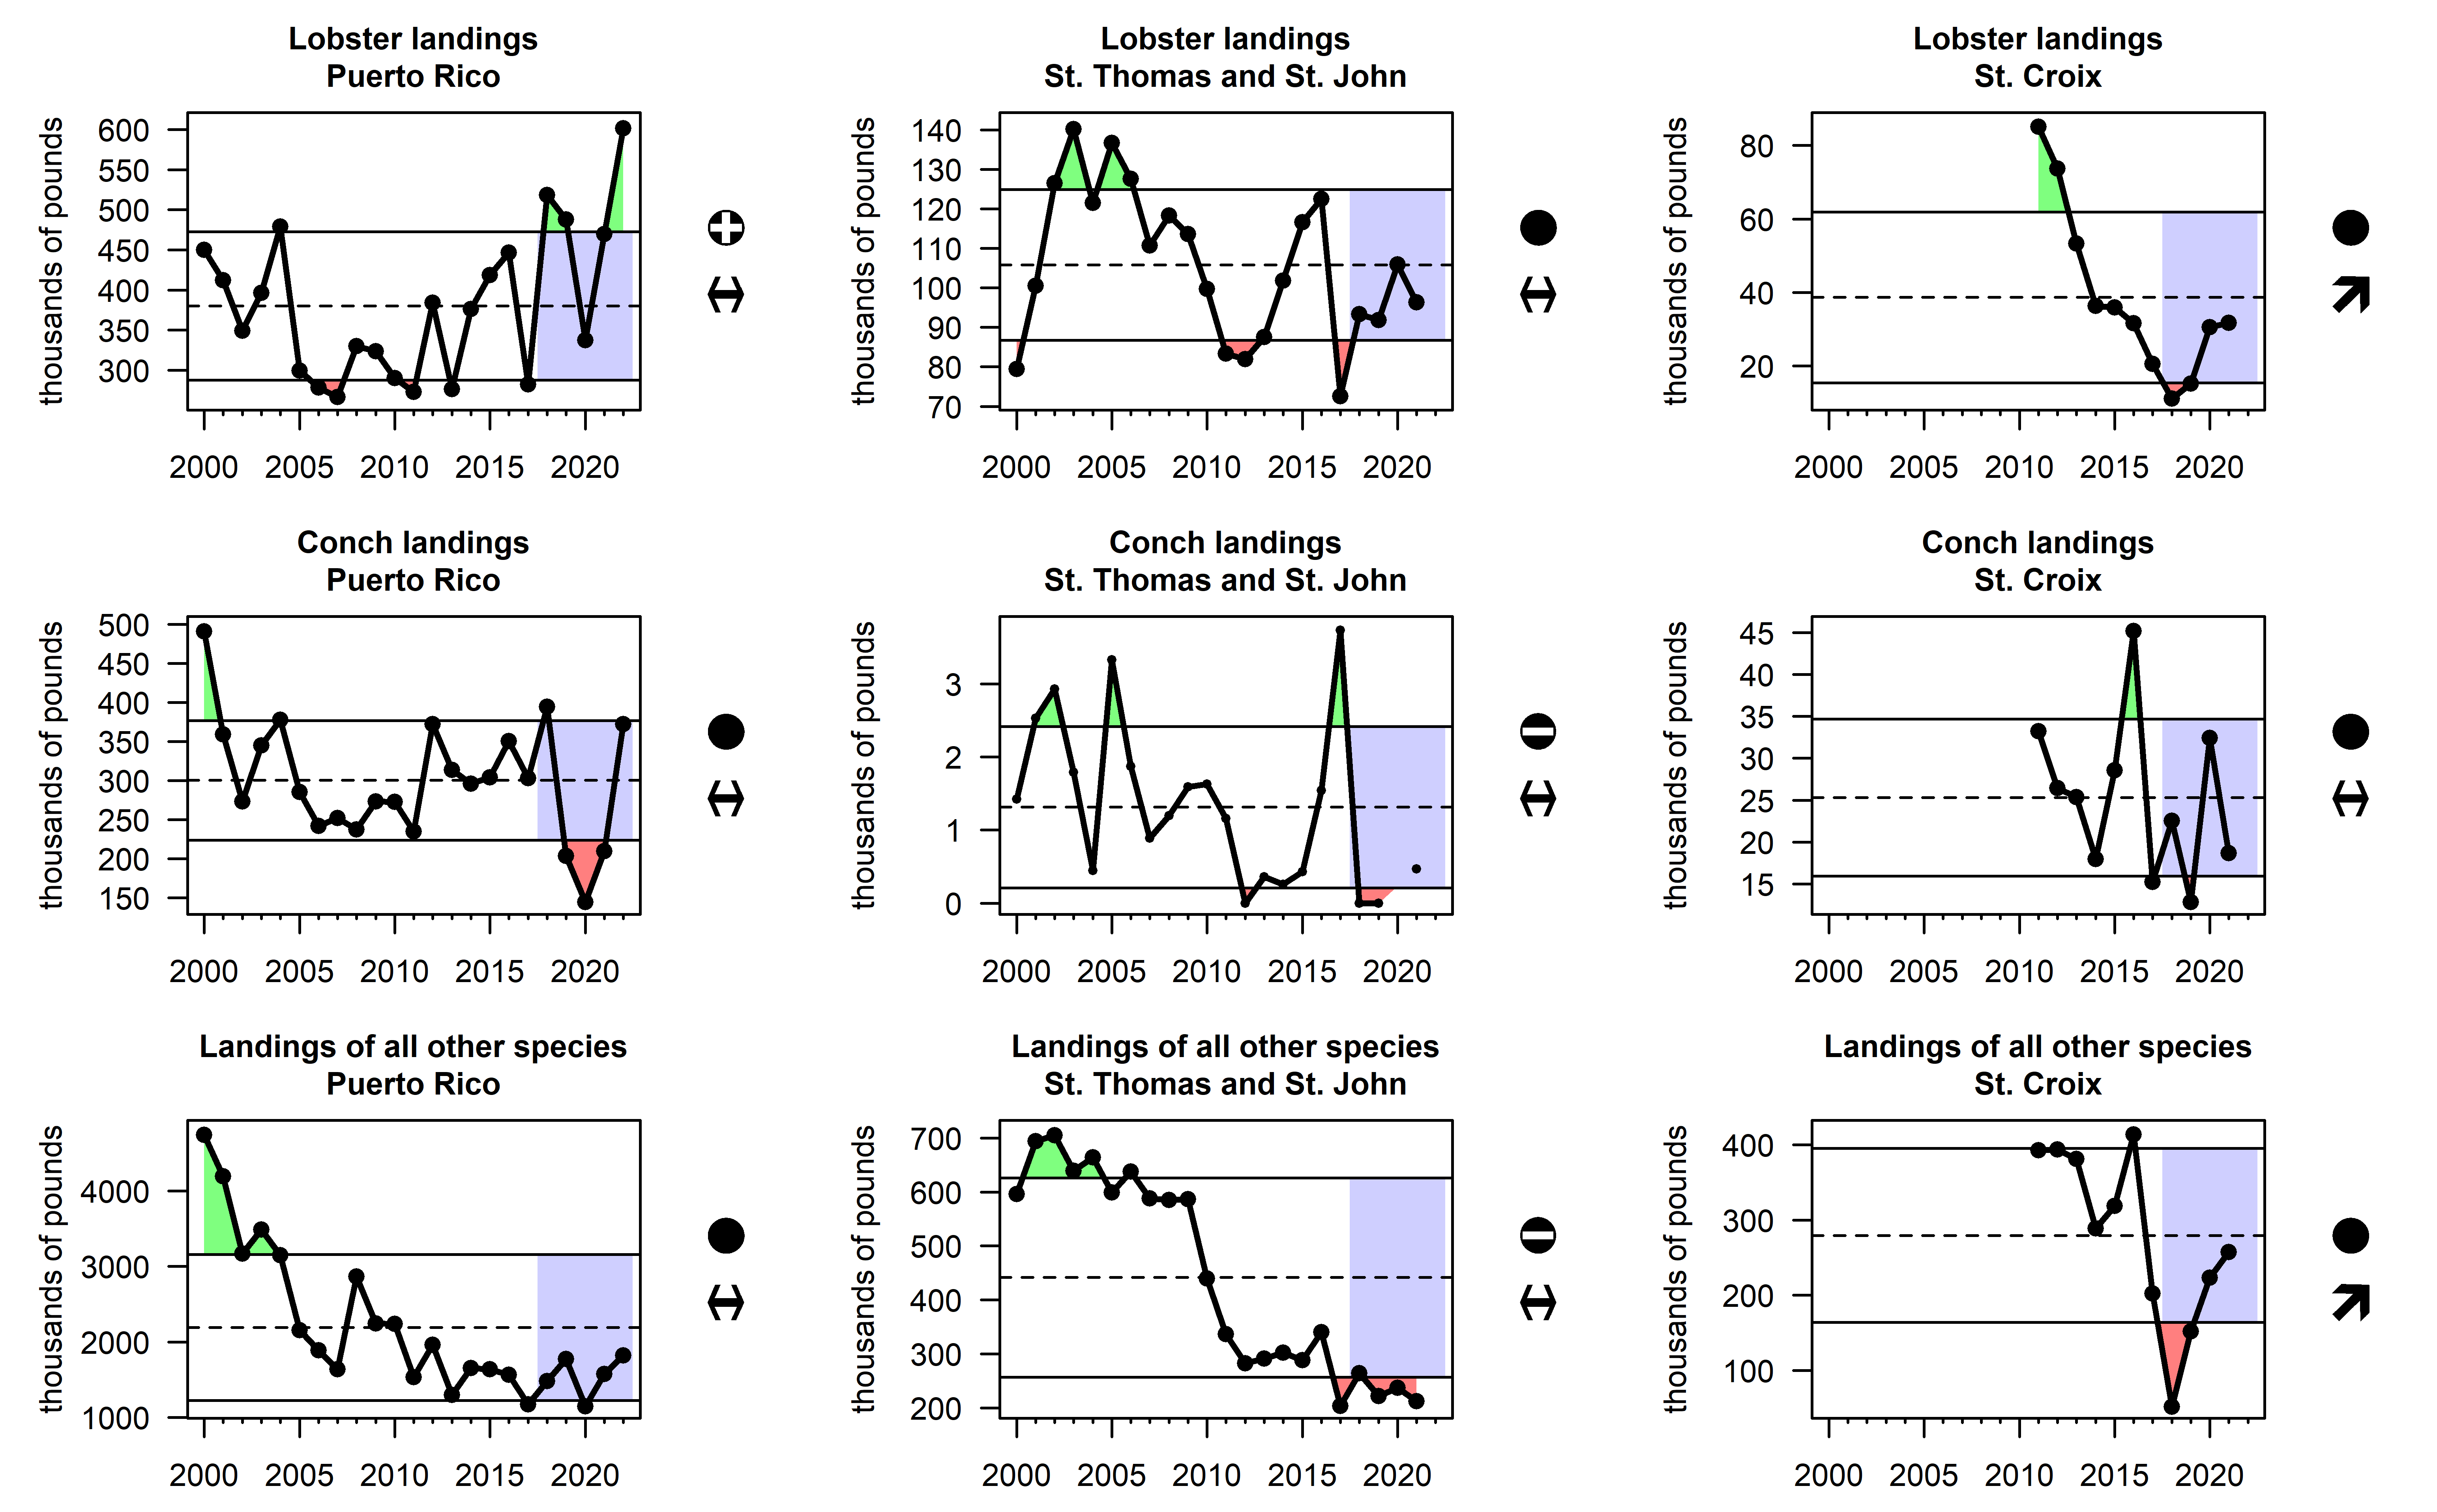
\includegraphics[keepaspectratio]{indicator_plots/total_landings_plot_final.png}}

}

\caption{\label{fig-totalland}Total landings of lobsters (top row),
conch (middle row), and all other commercial species (bottom row) from
commercial landings data in Puerto Rico (left column), St.~Thomas and
St.~John (middle column) and St.~Croix (right column). Confidential
landings appear as missing values. Note that the years in the USVI are
fishing years (July 1st to June 30th of the following year).}

\end{figure}%

\section{Socioeconomic health}\label{socioeconomic-health}

\subsection{Commercial revenues}\label{commercial-revenues}

The relative revenue contribution to commercial fisheries by species
conveys the changing reliance on different species across the U.S.
Caribbean. Revenues were calculated from the Caribbean Commercial
Landings data based on the weight of landings in each trip and the
reported price; anomalously high prices and missing values were replaced
by the overall average price for the given species group. In Puerto
Rico, approximately a third of the revenues have consistently come from
snapper species; this is followed by lobster and conch, which were both
increasing in their revenue contribution up to 2017
(Figure~\ref{fig-perlandPR}). In St.~Thomas and St.~John, there has also
been increasing dependence on lobster, which supplies roughly a third of
the revenues for those islands (Figure~\ref{fig-perlandSTT}). Revenues
in St.~Croix are not dominated by a single species group; parrotfishes,
tunas and mackerels, lobsters, snappers, and dolphinfish make up
approximately 75\% of the revenues (Figure~\ref{fig-perlandSTX}).

\begin{figure}

\centering{

\pandocbounded{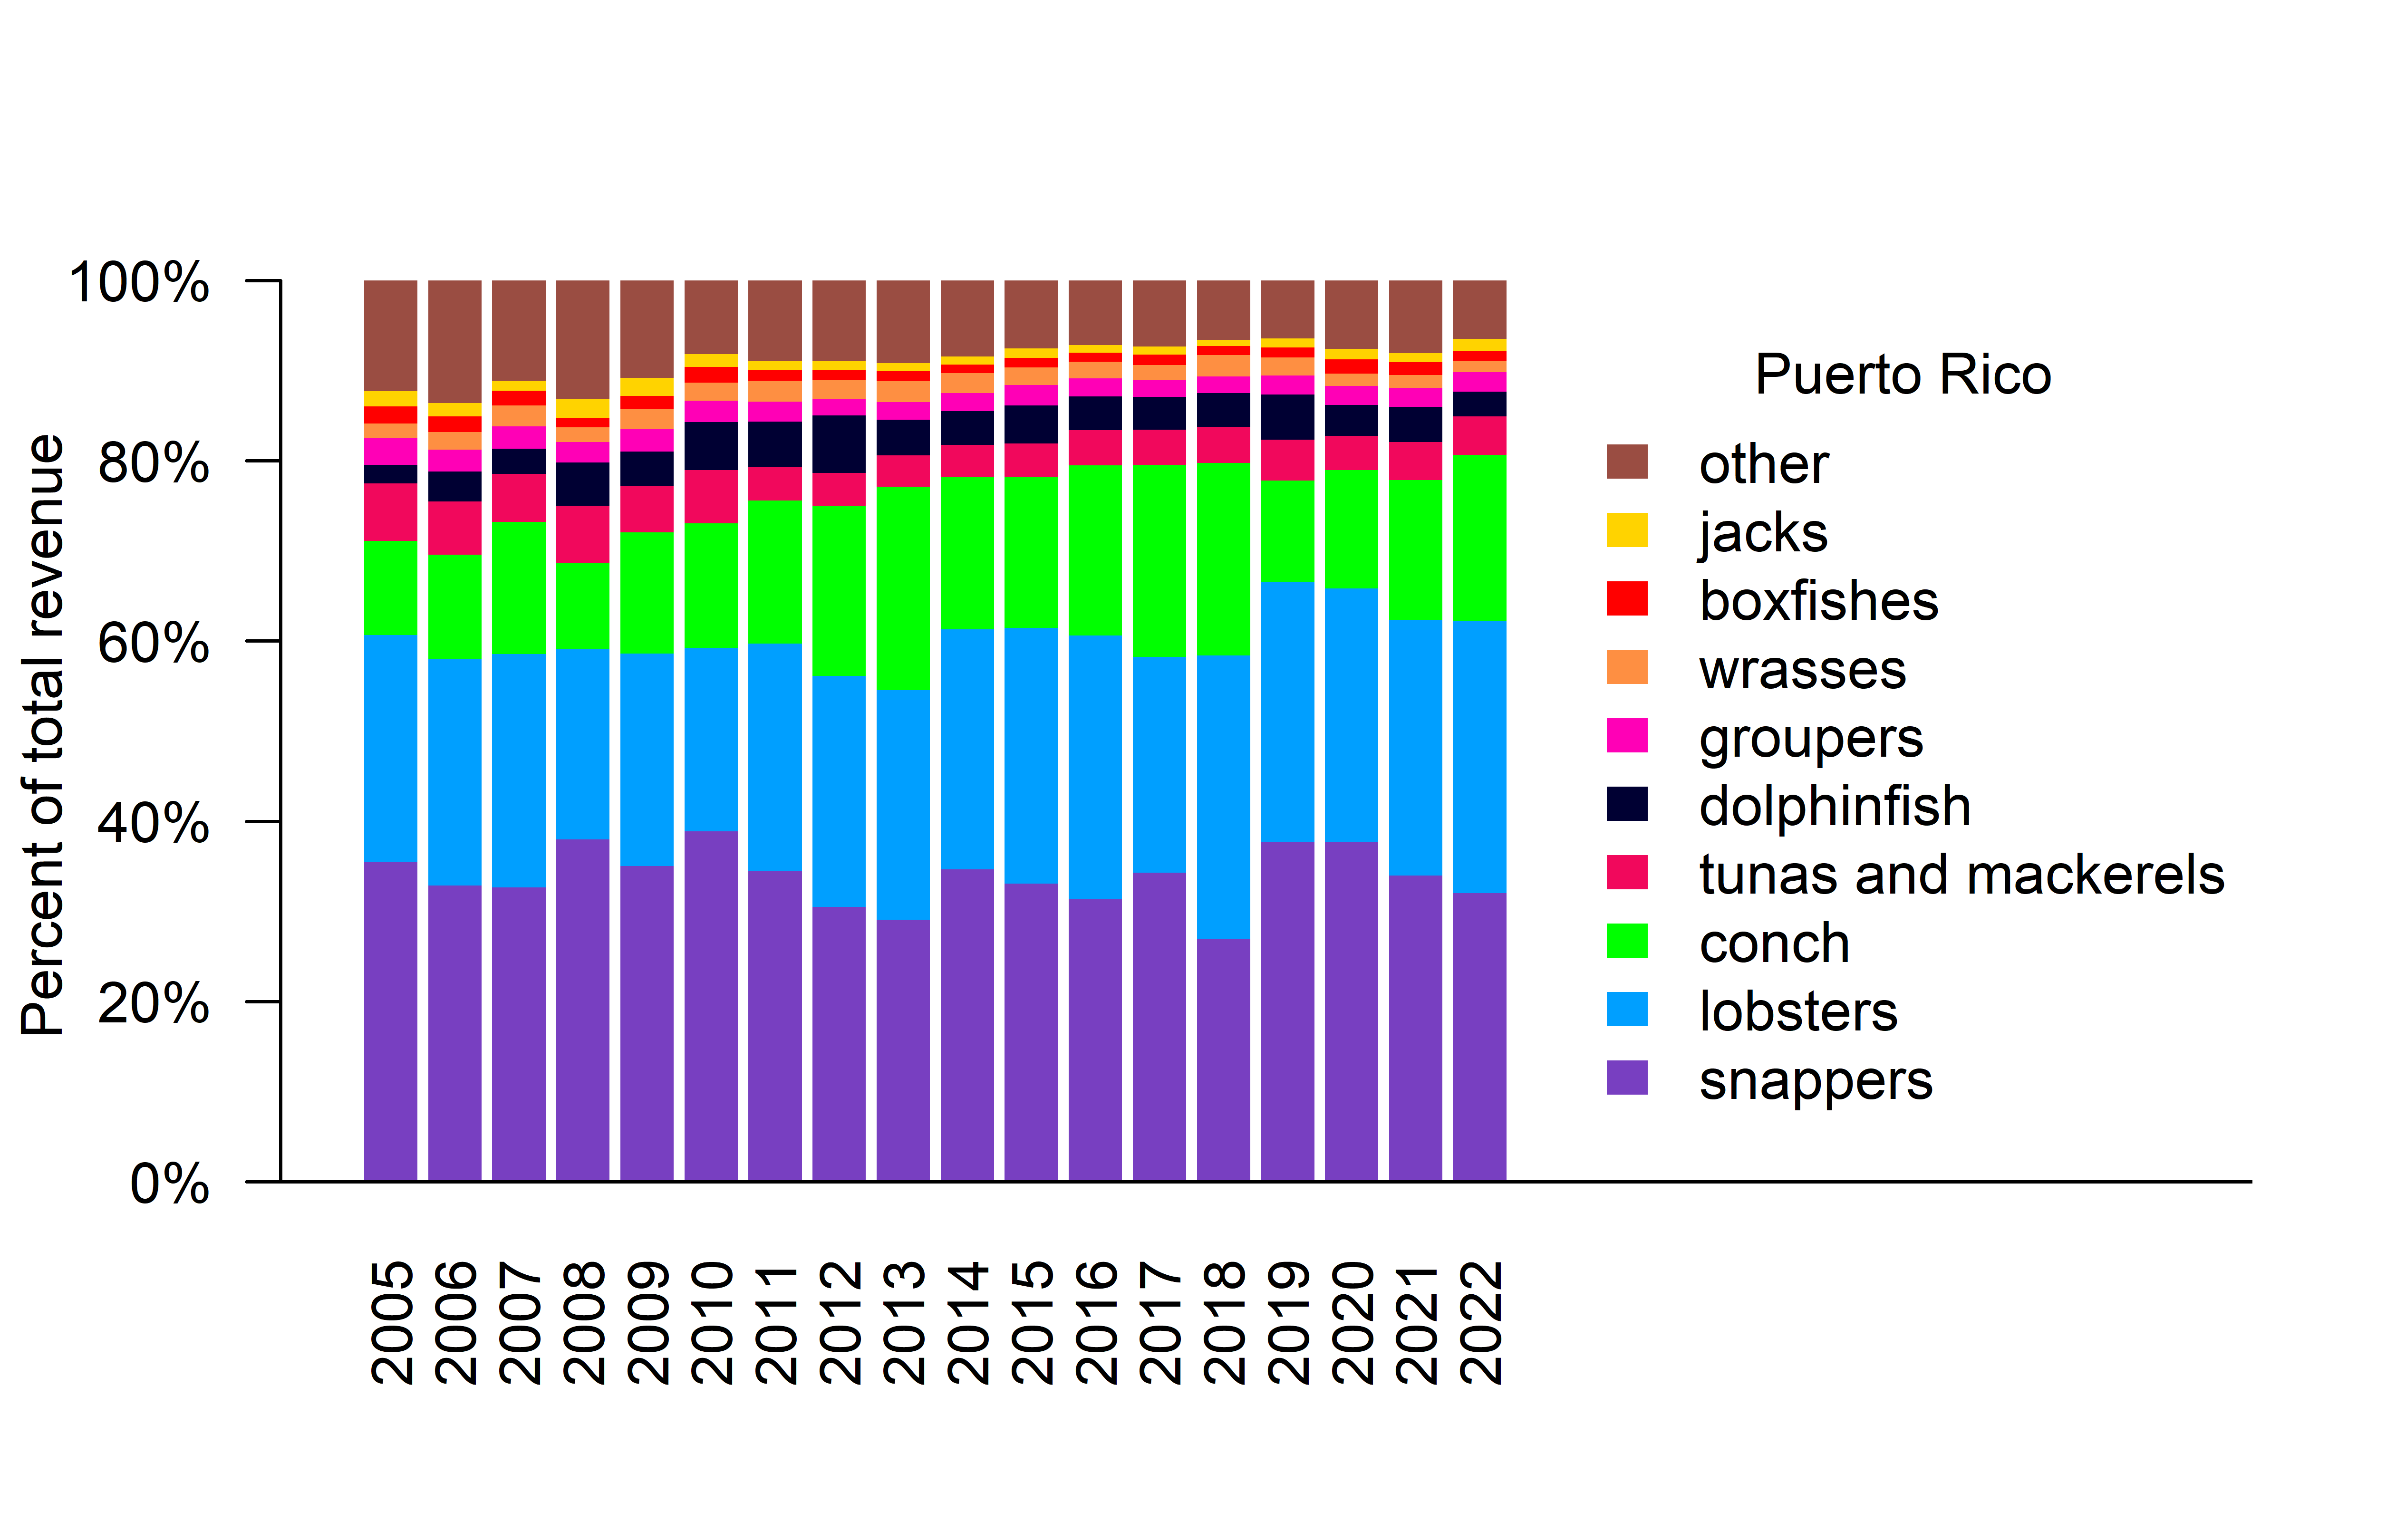
\includegraphics[keepaspectratio]{indicator_plots/per_landings_PR.png}}

}

\caption{\label{fig-perlandPR}Percent revenue contribution for the top
ten species groups, stacked by their order of overall importance, for
commercial fisheries in Puerto Rico.}

\end{figure}%

\begin{figure}

\centering{

\pandocbounded{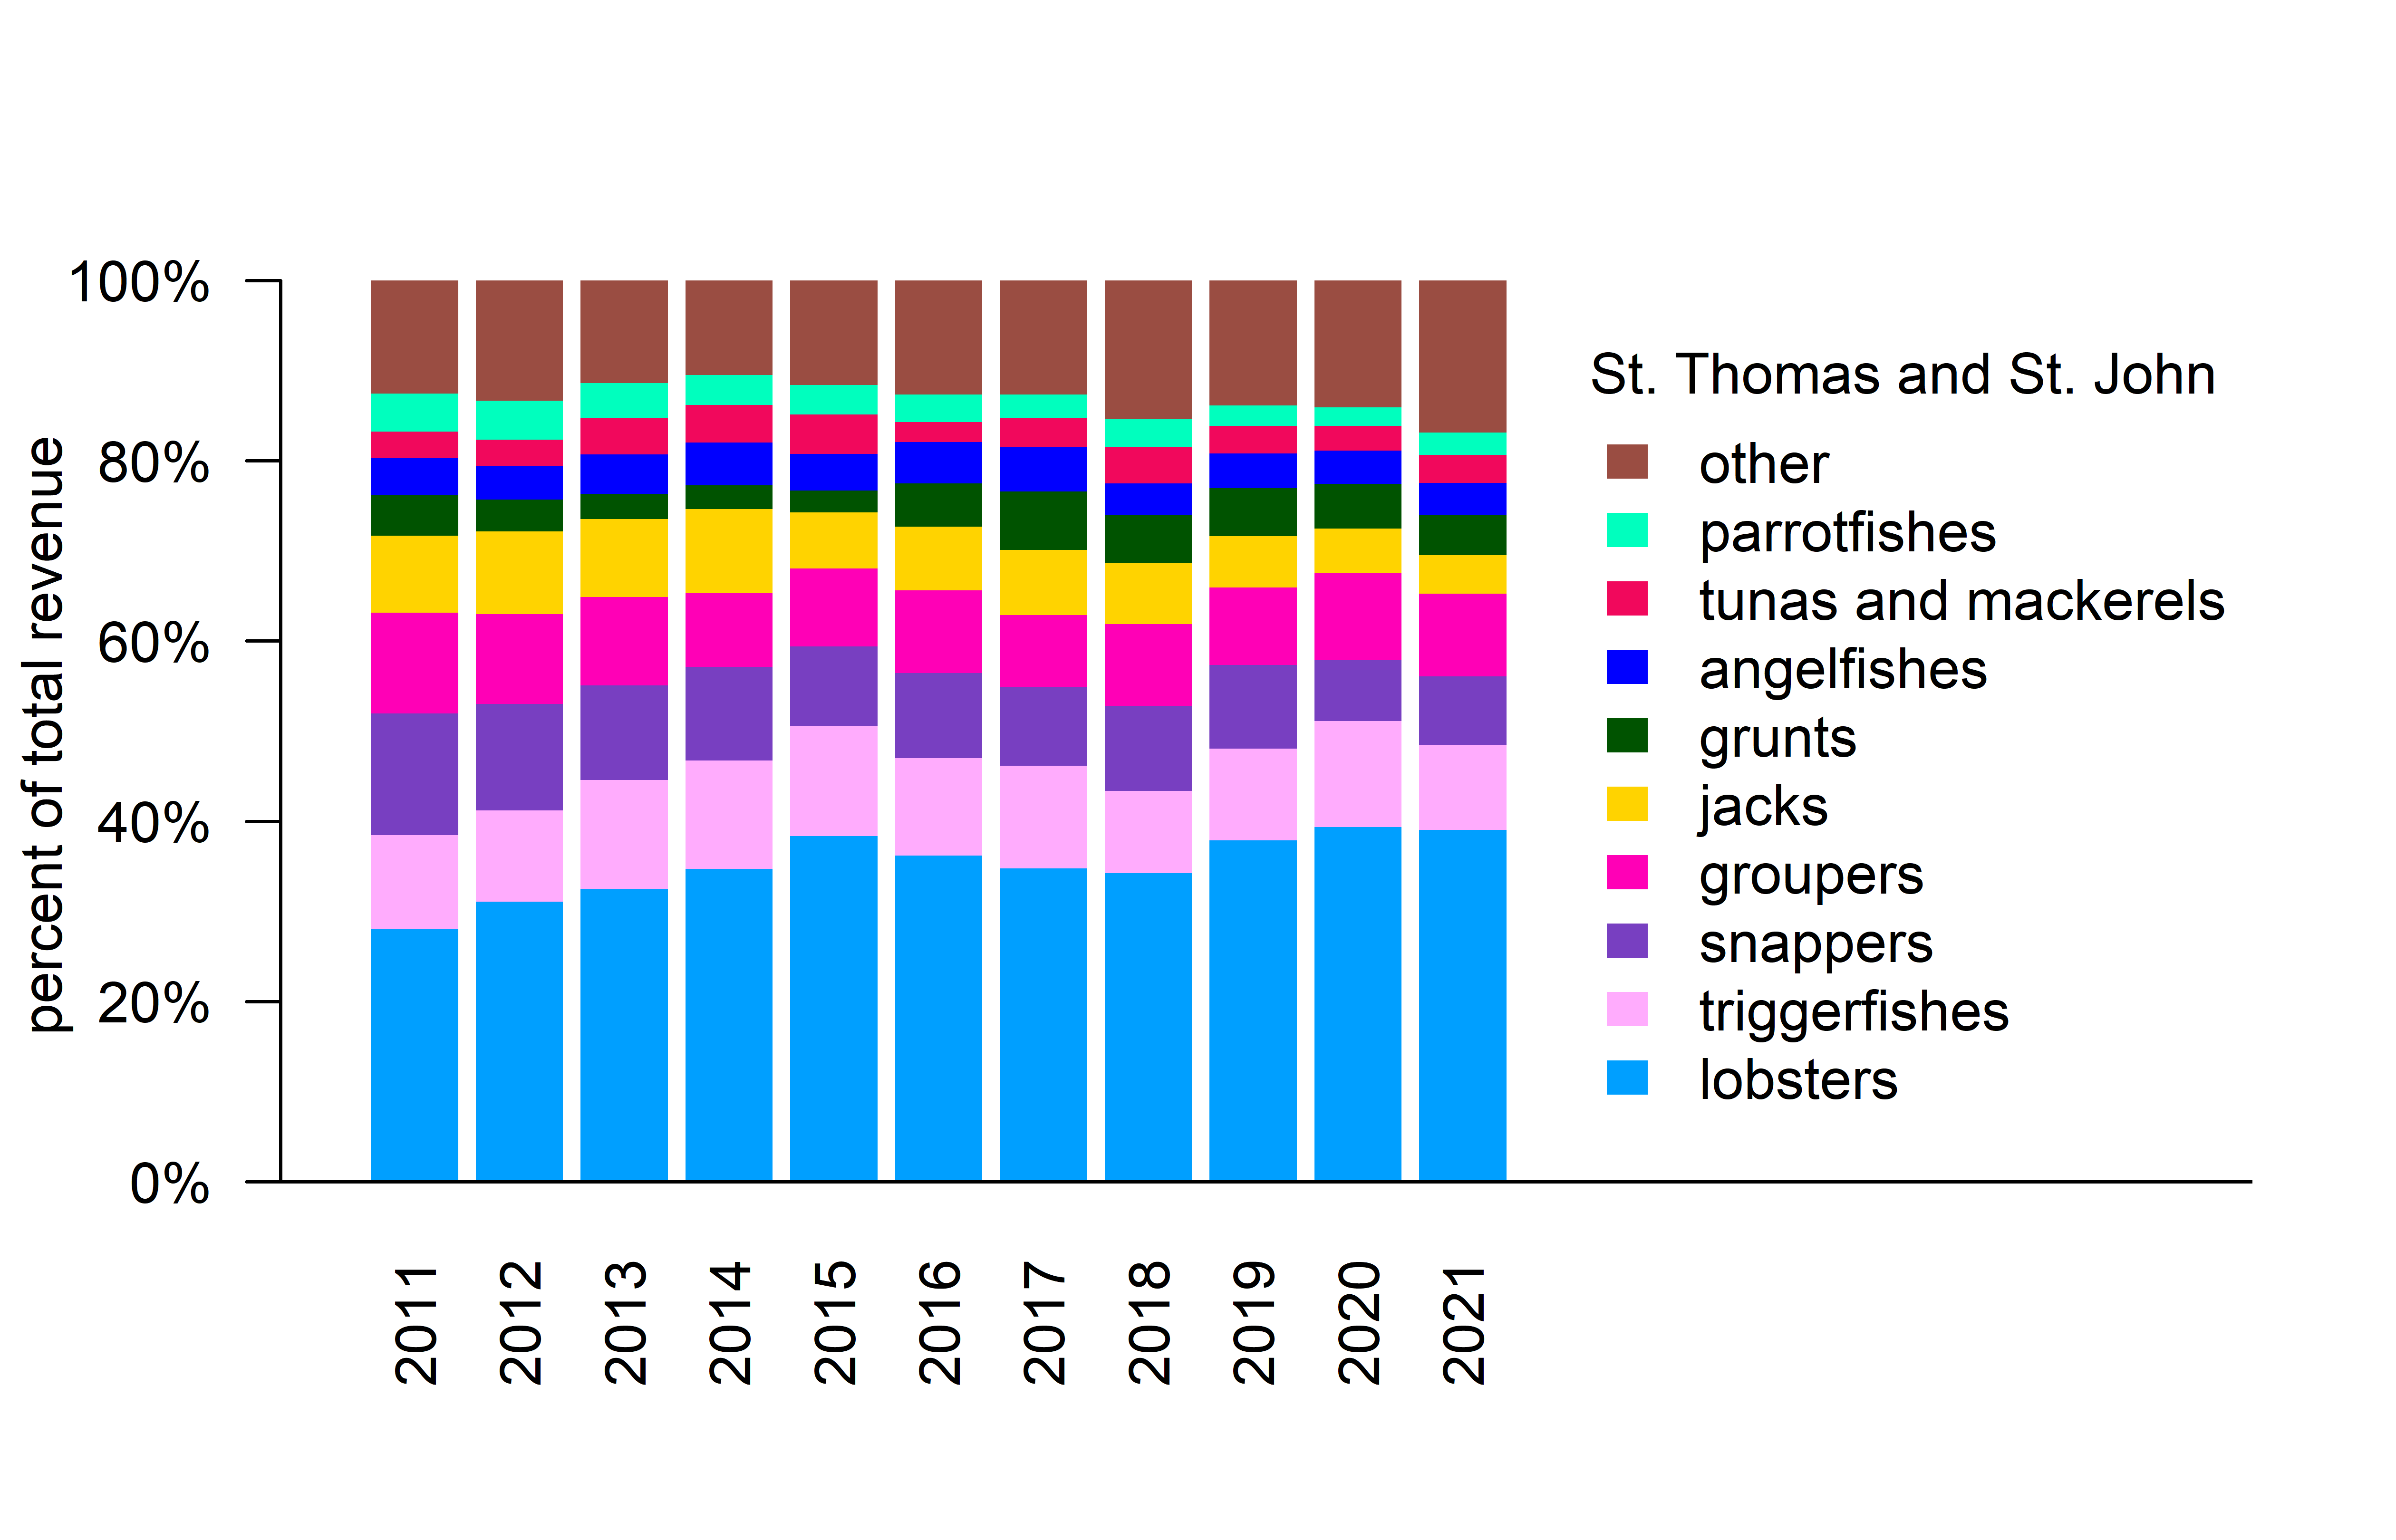
\includegraphics[keepaspectratio]{indicator_plots/per_landings_STT.png}}

}

\caption{\label{fig-perlandSTT}Percent revenue contribution for the top
ten species groups, stacked by their order of overall importance, for
commercial fisheries in St.~Thomas and St.~John. Note that the years are
fishing years (July 1st to June 30th of the following year).}

\end{figure}%

\begin{figure}

\centering{

\pandocbounded{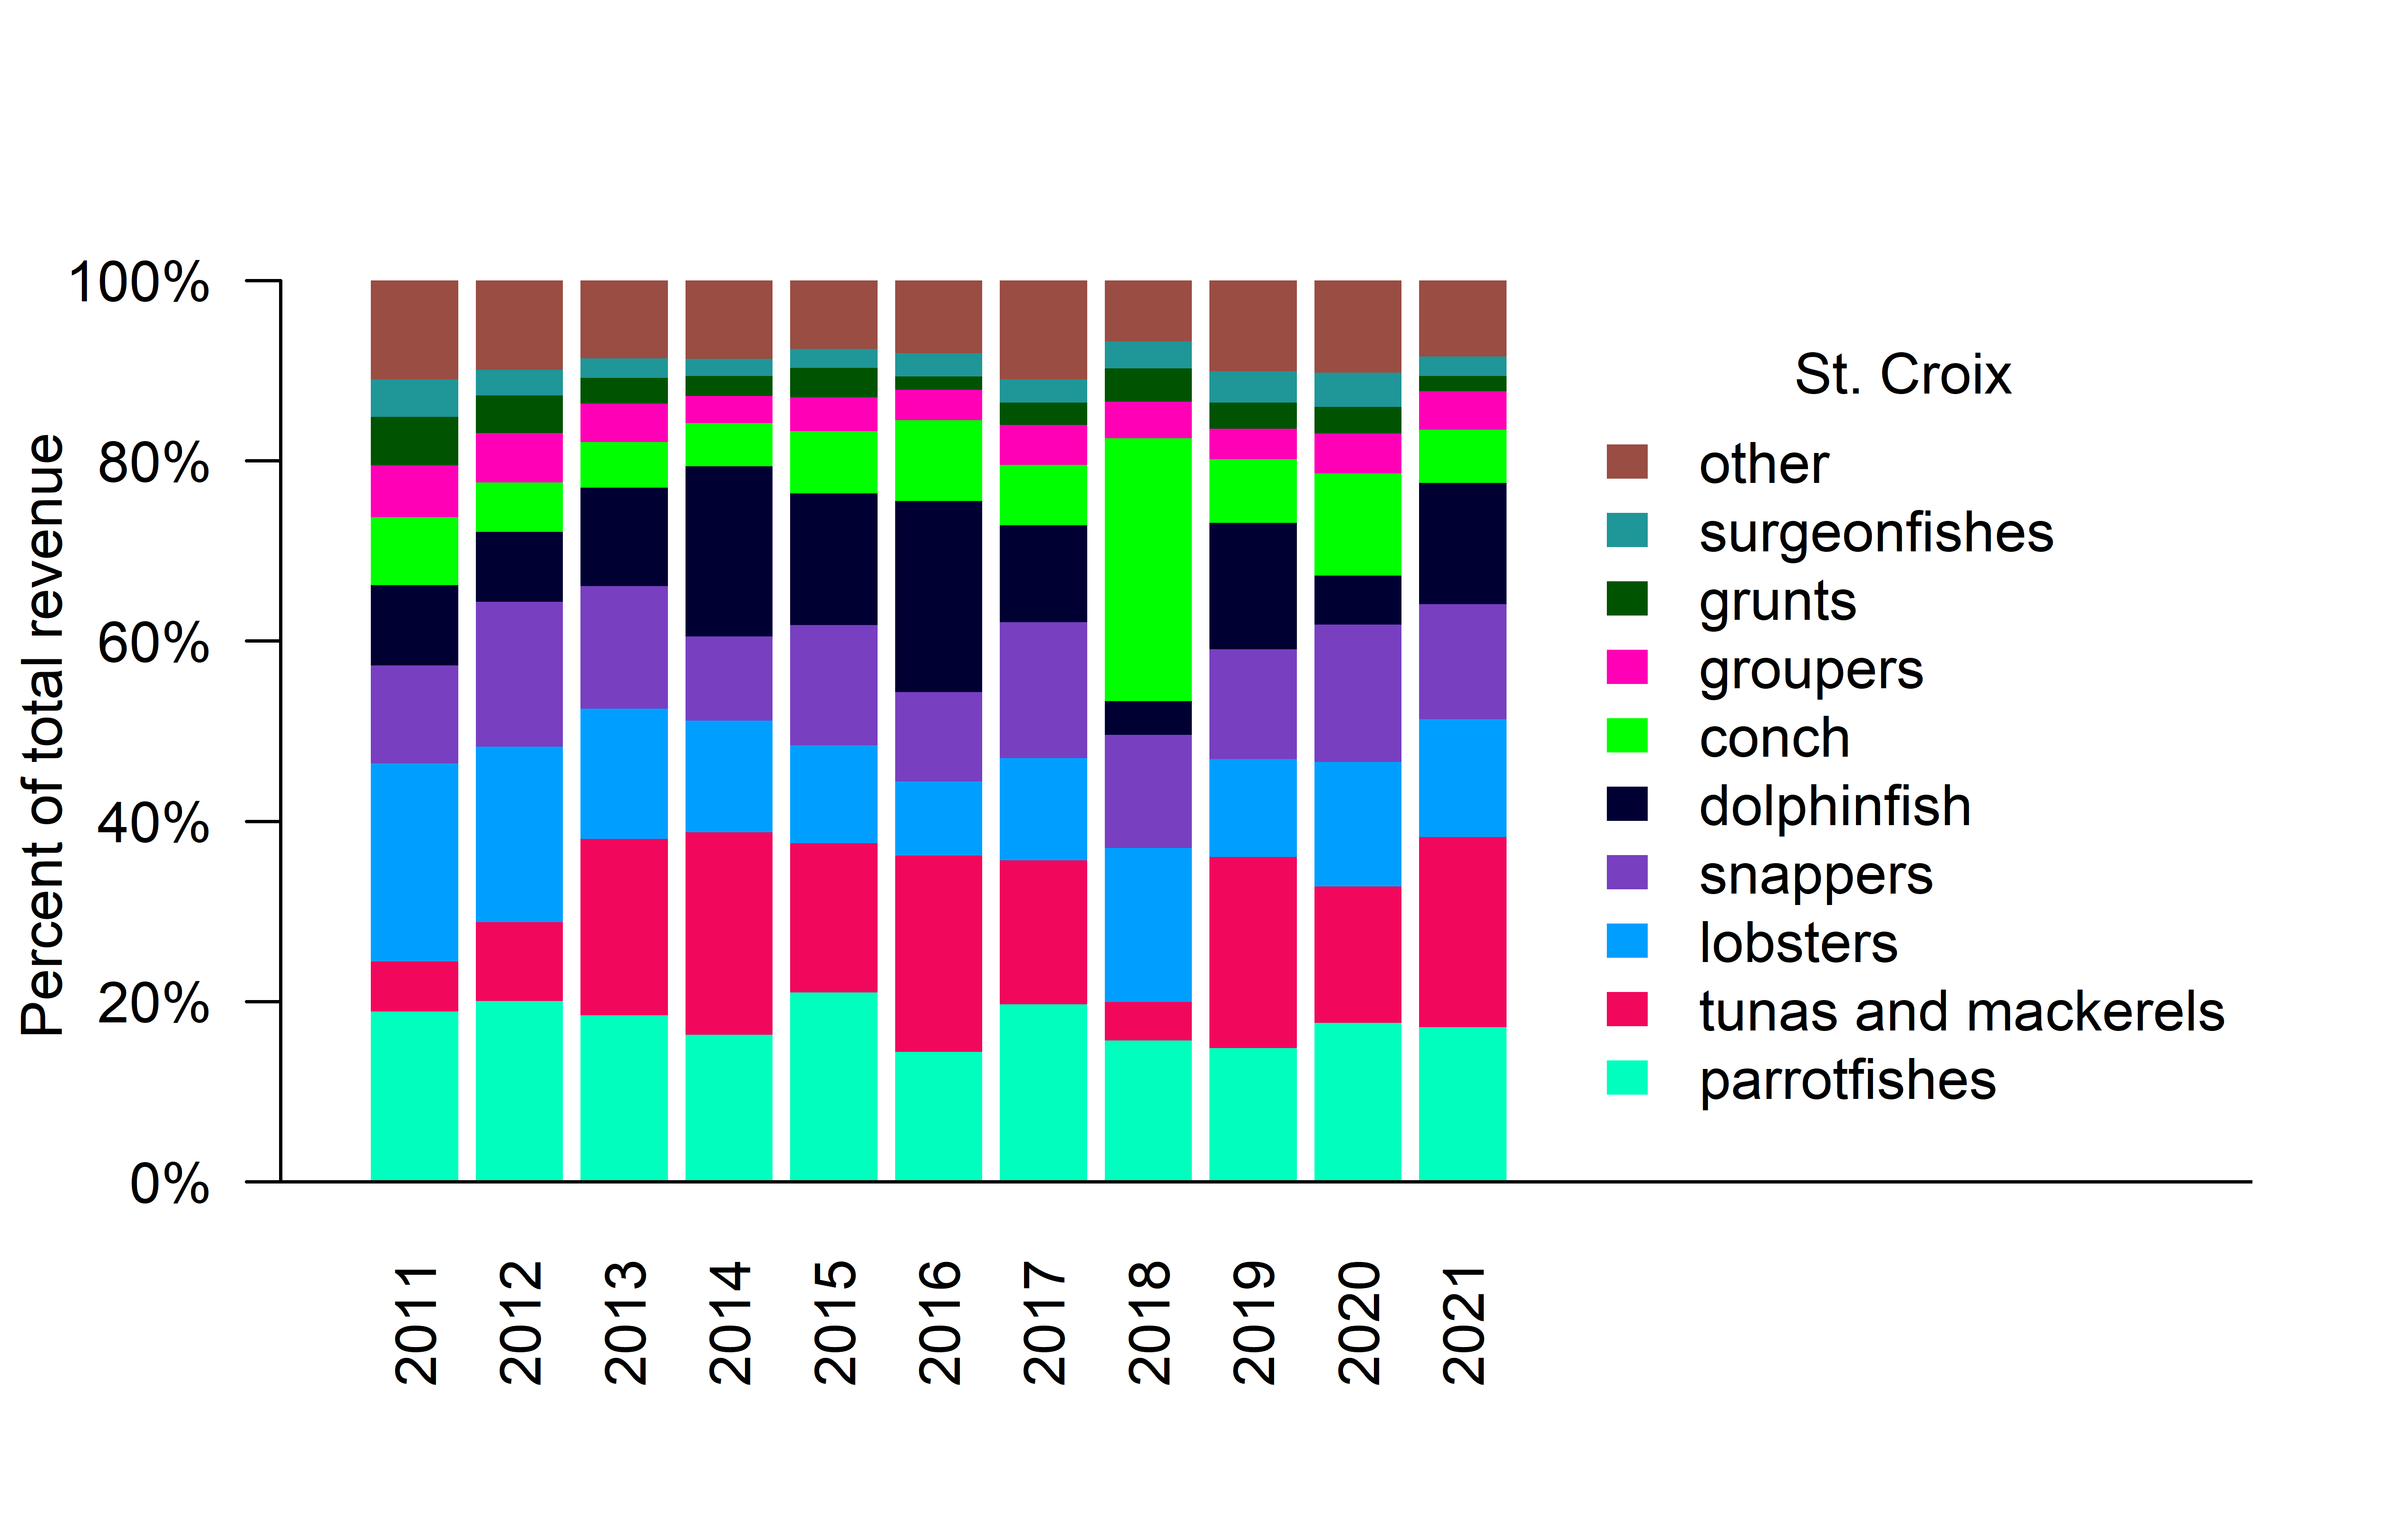
\includegraphics[keepaspectratio]{indicator_plots/per_landings_STX.png}}

}

\caption{\label{fig-perlandSTX}Percent revenue contribution for the top
ten species groups, stacked by their order of overall importance, for
commercial fisheries in St.~Croix. Note that the years are fishing years
(July 1st to June 30th of the following year).}

\end{figure}%

\subsection{Commercial fishing trips}\label{commercial-fishing-trips}

Commercial fishing trips are a useful socioeconomic indicator because
they capture the amount and type of effort, which may be driven by
market factors, regulations, and costs of entering the fishery. The
total number of trips, broken down by gear type, was extracted from the
Caribbean Commercial Landings database by identifying unique trips based
on date and vessel number and extracting the primary reported gear used
for each trip. In Puerto Rico, trip numbers have generally decreased
over time, with marked decreases in 2017 and 2020; sudden changes in the
hook and line fishing in 2012 are due to changes in reporting forms
(Figure~\ref{fig-gearPR}). Effort has similarly declined in St.~Thomas
and St.~John; marked declines after 2010 are likely due to reduced
reporting (Figure~\ref{fig-gearSTT}). Similarly, in St.~Croix the number
of trips has declined, with the 2018--2019 fishing season reporting
particularly low effort (Figure~\ref{fig-gearSTX}). Gear types are
plotted using the same order and color codes, to facilitate comparisons
among the islands.

\begin{figure}

\centering{

\pandocbounded{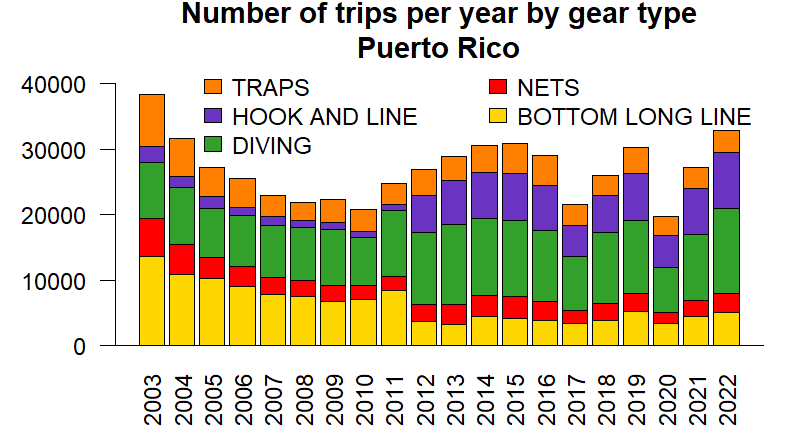
\includegraphics[keepaspectratio]{indicator_plots/gearTypes_PR.png}}

}

\caption{\label{fig-gearPR}Total number of commercial fishing trips by
gear type in Puerto Rico, separated by primary gear used on the trip.}

\end{figure}%

\begin{figure}

\centering{

\pandocbounded{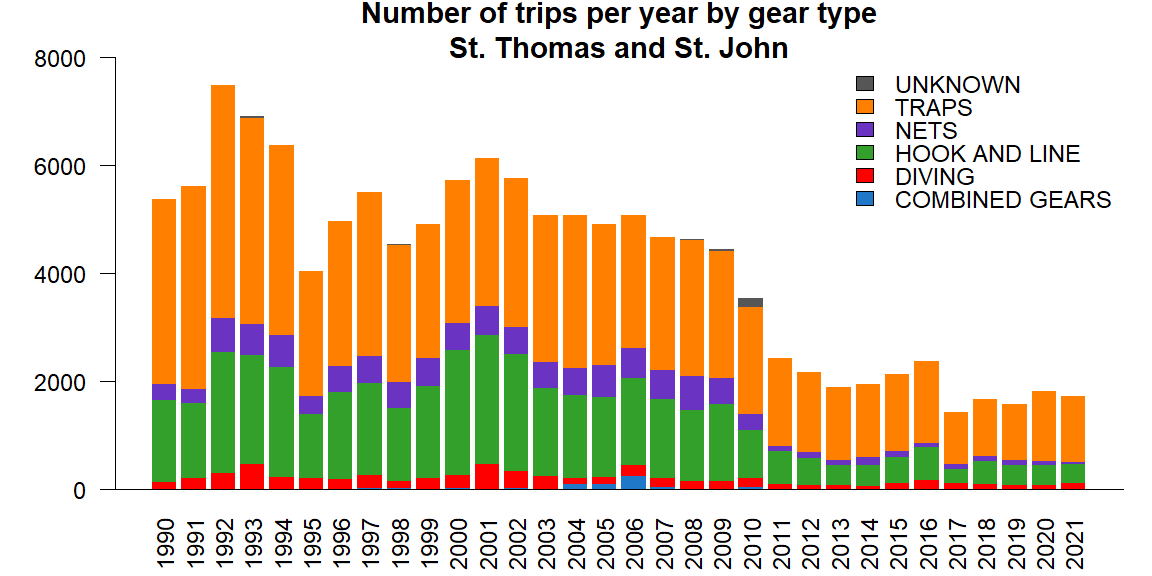
\includegraphics[keepaspectratio]{indicator_plots/gearTypes_STT.png}}

}

\caption{\label{fig-gearSTT}Total number of commercial fishing trips by
gear type in St.~Thomas and St.~John, separated by primary gear used on
the trip. Note that the years are fishing years (July 1st to June 30th
of the following year).}

\end{figure}%

\begin{figure}

\centering{

\pandocbounded{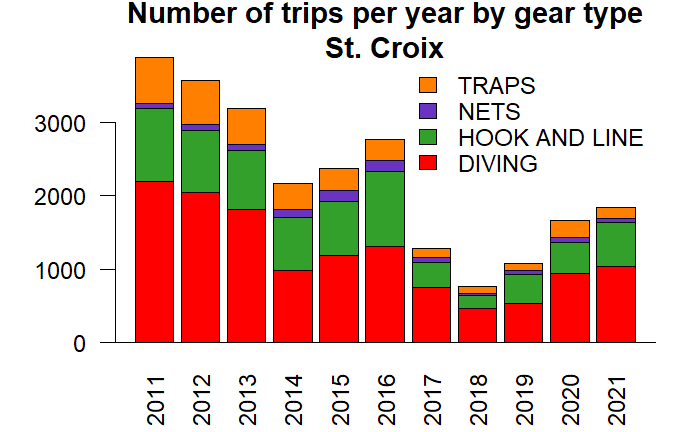
\includegraphics[keepaspectratio]{indicator_plots/gearTypes_STX.png}}

}

\caption{\label{fig-gearSTX}Total number of commercial fishing trips by
gear type in St.~Croix, separated by primary gear used on the trip. Note
that the years are fishing years (July 1st to June 30th of the following
year).}

\end{figure}%

Given the potential for changes in reporting to impact trip numbers, it
can more informative to look at the composition of gear types. In
particular, diving is often a way of entry for new or part-time
fishermen as it generally requires lower up-front investments. Peaks in
the proportion diving trips in 2017 and 2018 could be a result of lost
traps and infrastructure due to hurricanes (Figure~\ref{fig-dive}).

\begin{figure}

\centering{

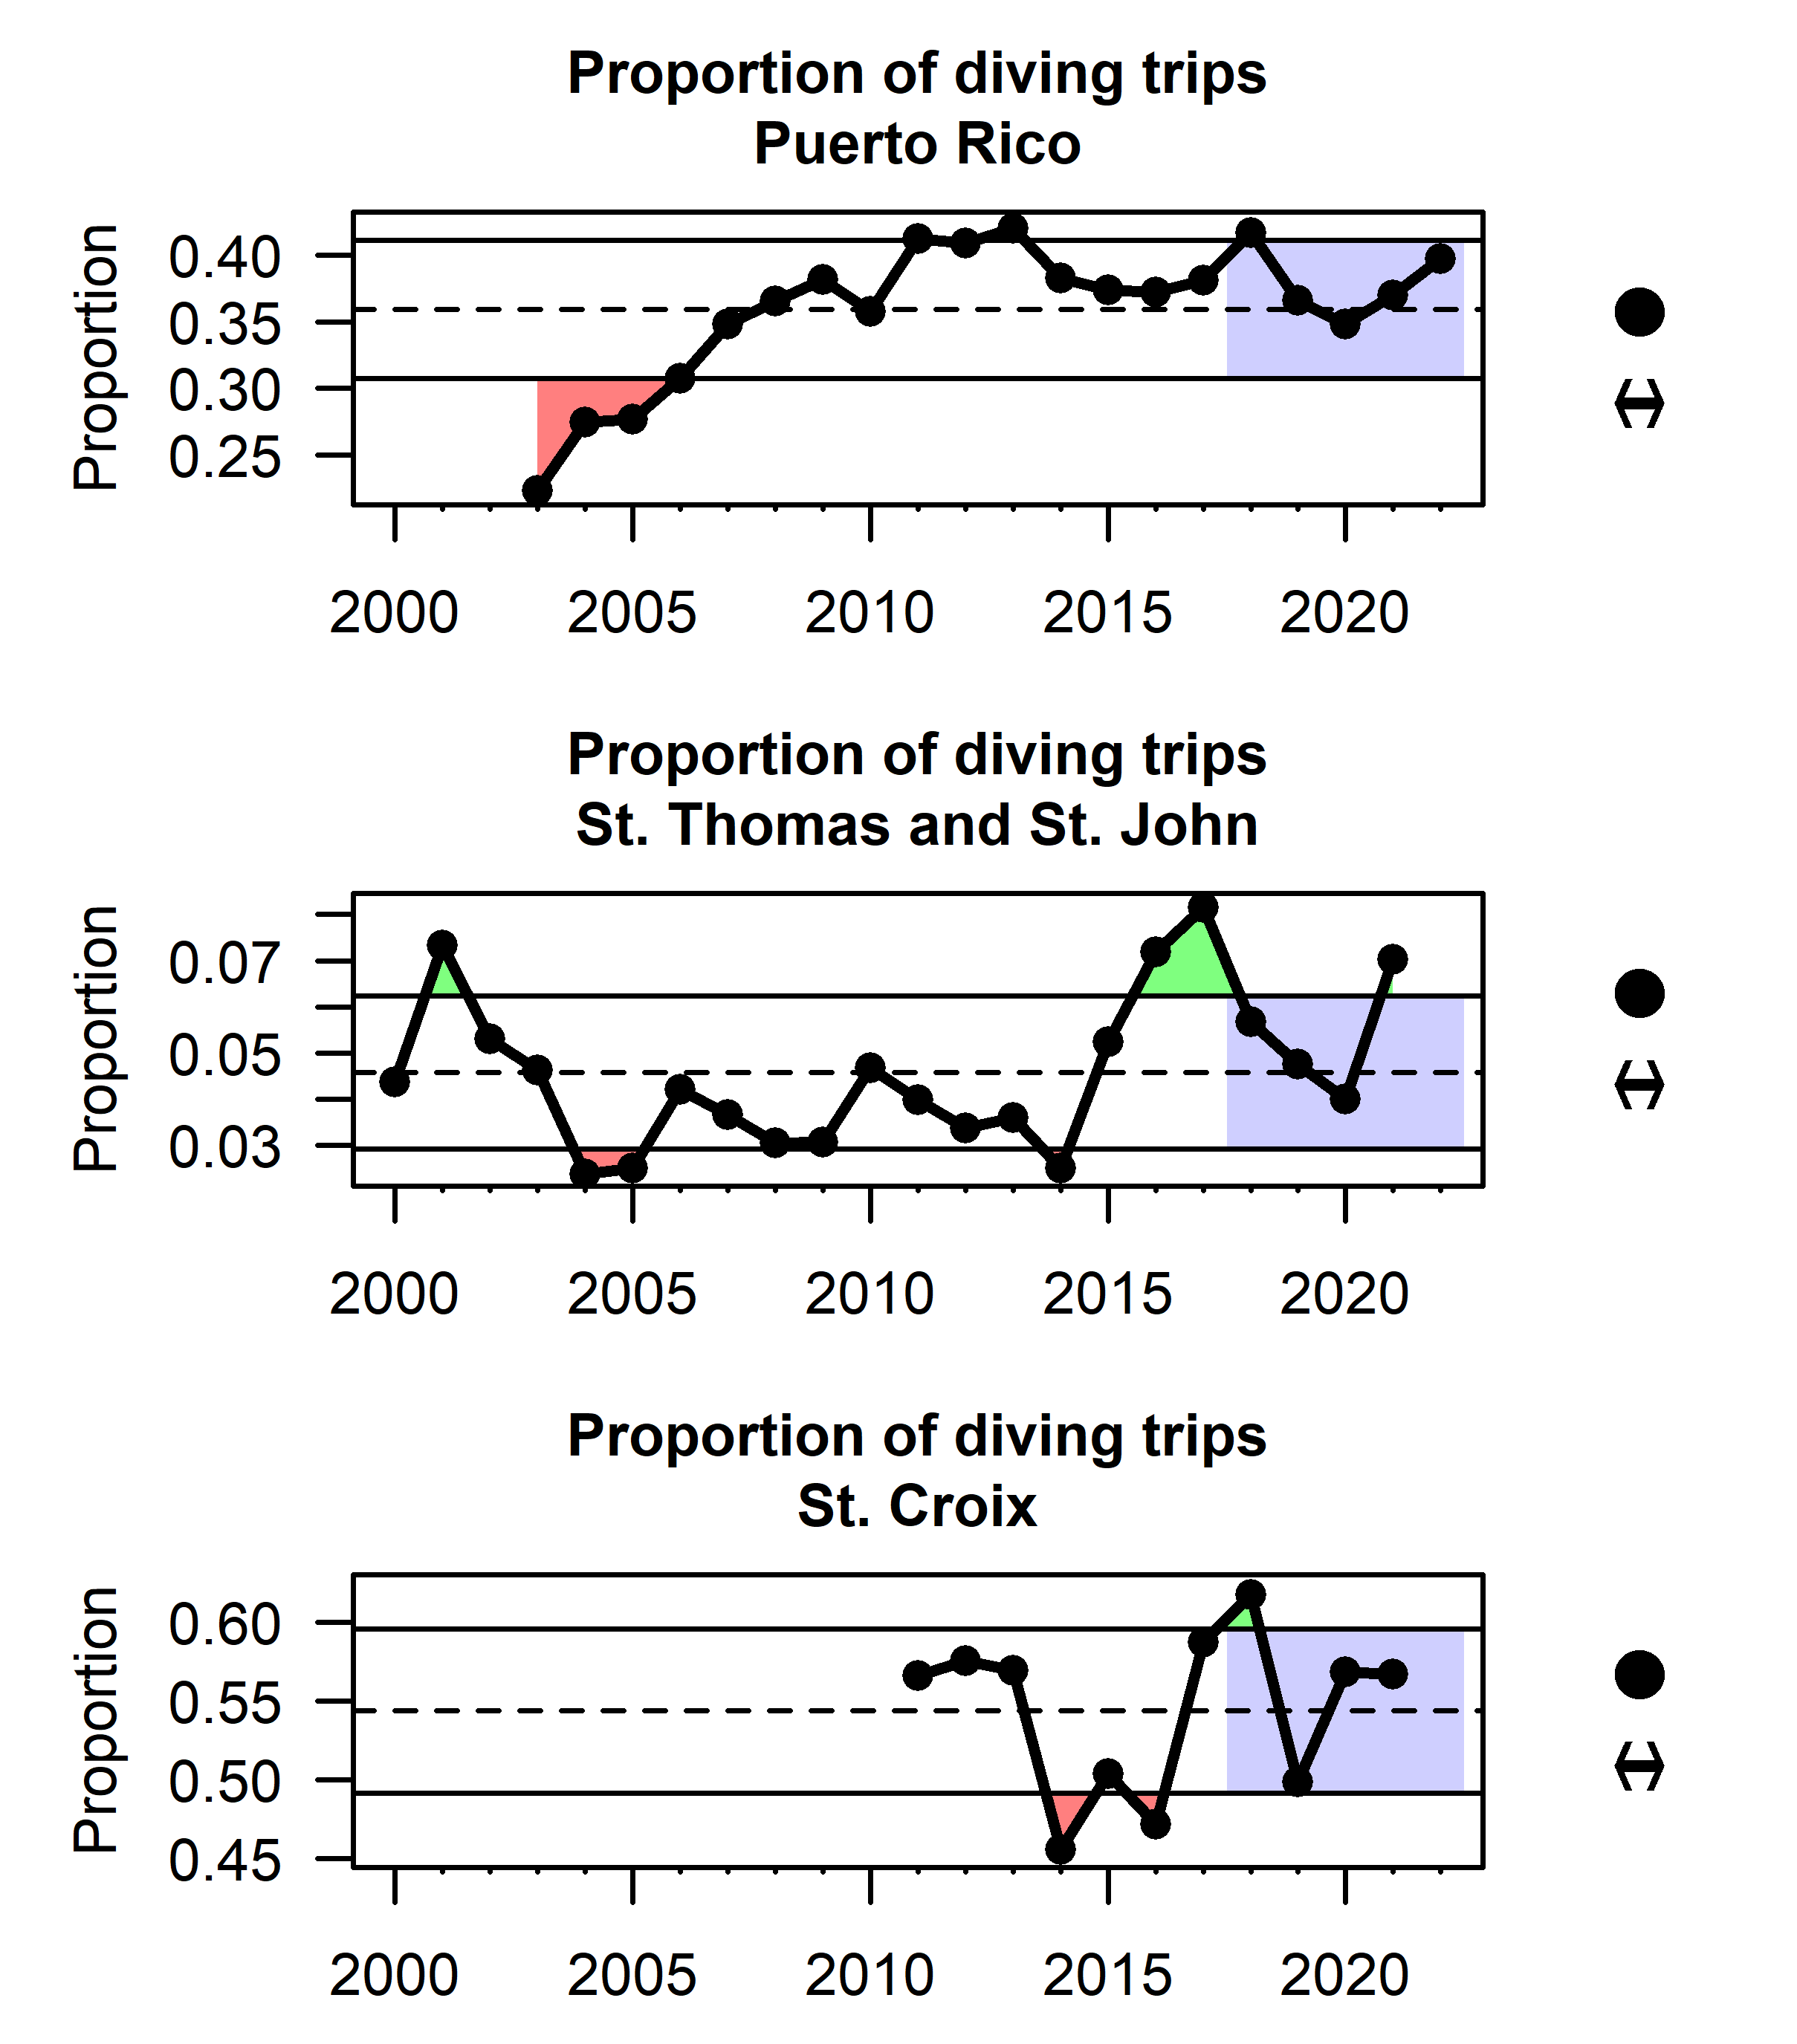
\includegraphics[width=0.75\linewidth,height=\textheight,keepaspectratio]{indicator_plots/prop_diving_trips_plot_final.png}

}

\caption{\label{fig-dive}Proportion of commercial trips that are
reported as diving trips for Puerto Rico (top), St.~Thomas and St.~John
(middle) and St.~Croix (bottom). Note that the years in the USVI are
fishing years (July 1st to June 30th of the following year).}

\end{figure}%

Ordination of gear types based on reporting landing sites conveys how
different regions across the U.S. Caribbean depend on different methods
of fishing. Ordinations were conducting using non-metric
multidimensional scaling (NMDS) based on matrices representing the
proportion of gear types used by landing site. The NMDS algorithm seeks
to place different sites in an X-dimensional space, such that the
physical distances between each pair of sites best represents the
differences in gear types employed. Thus, sites that appear more closely
together in the figures are more similar in their gear usage, and the
position of the gear type labels denote the relative importance of those
gear types in those sites. In Puerto Rico for example, hook and line and
bottom long line are closely related and are particularly prevalent in
the northern landing sites (in red), whereas nets and traps are more
prevalent in the South (blue) (Figure~\ref{fig-NMDSPR}). In St.~Thomas
and St.~John, there is an association of traps and hook and line fishing
(Figure~\ref{fig-NMDSSTT}), whereas in St.~Croix, those gear types are
not associated with each other but nets and spearfishing are closely
associated within landing sites (Figure~\ref{fig-NMDSSTX}).

\begin{figure}

\centering{

\pandocbounded{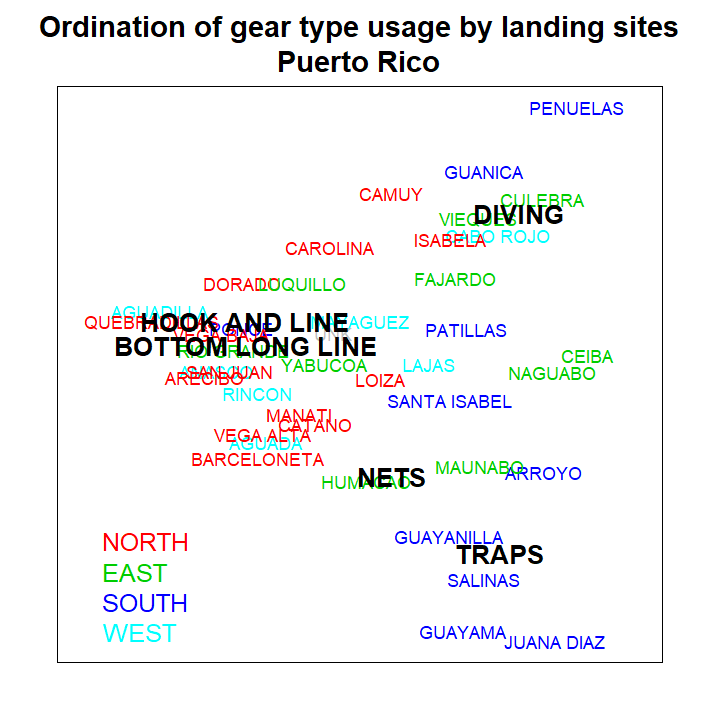
\includegraphics[keepaspectratio]{indicator_plots/NMDSgear_PR.png}}

}

\caption{\label{fig-NMDSPR}Ordination of gear type usage by landing site
for Puerto Rico, color coded by region.}

\end{figure}%

\begin{figure}

\centering{

\pandocbounded{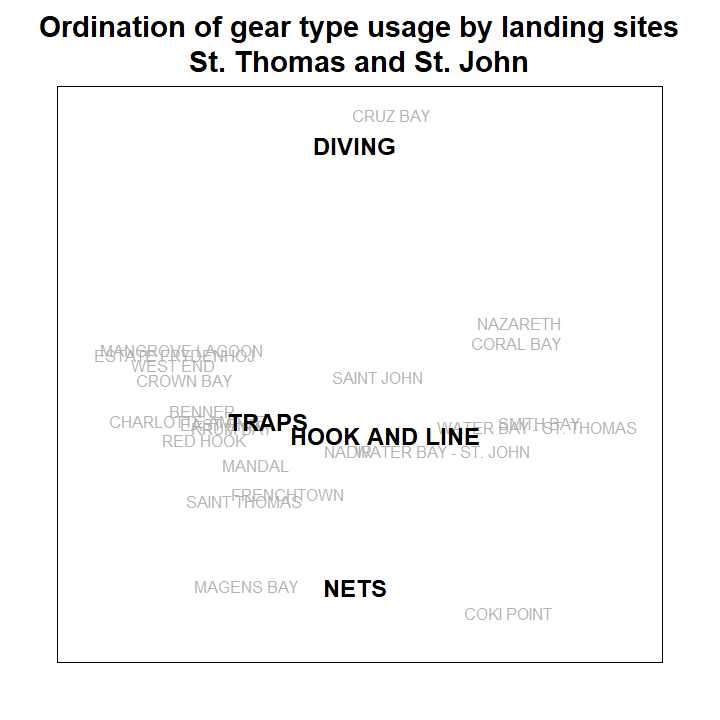
\includegraphics[keepaspectratio]{indicator_plots/NMDSgear_STT.png}}

}

\caption{\label{fig-NMDSSTT}Ordination of gear type usage by landing
site for St.~Thomas and St.~John.}

\end{figure}%

\begin{figure}

\centering{

\pandocbounded{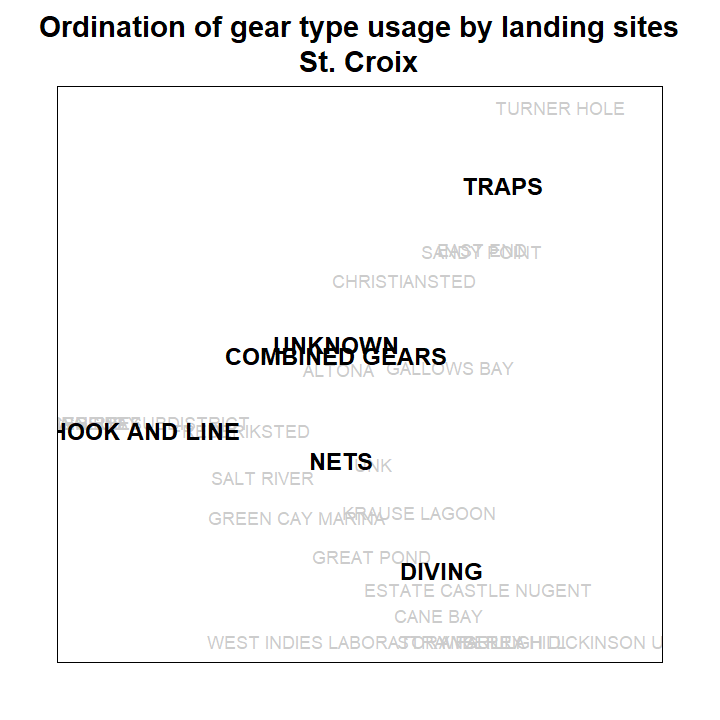
\includegraphics[keepaspectratio]{indicator_plots/NMDSgear_STX.png}}

}

\caption{\label{fig-NMDSSTX}Ordination of gear type usage by landing
site for St.~Croix.}

\end{figure}%

\subsection{Economic activity}\label{economic-activity}

Some indicators of economic activity come in the form of gross domestic
product (GDP) and employment trends. GDP data come from the World Bank,
and indicate an overall general economic expansion in Puerto Rico (World
Bank 2024a). GDP in the USVI (World Bank 2024b) declined substantially
from 2007--2014, but has been increasing steadily since
(Figure~\ref{fig-GDP}). Several key trends emerge when analyzing GDP in
the USVI, but the broader economic story is one of dependency on
external market forces and vulnerability to external shocks. The impact
of major disruptions, both natural and financial, has shaped the
territory's economy. For instance, the destruction caused by Hurricanes
Irma and Maria in 2017 introduced significant economic and social
challenges. Estimates based on USVI fiscal data indicate that public
revenues were cut in half following the storms, severely constraining
government capacity. This shock compounded pre-existing fiscal
pressures, as USVI public revenues had already been significantly
affected by the 2007--2009 Great Recession. Given that tourism serves as
a primary economic driver, the downturn in the aftermath of these events
further limited growth in the region.

\begin{figure}

\centering{

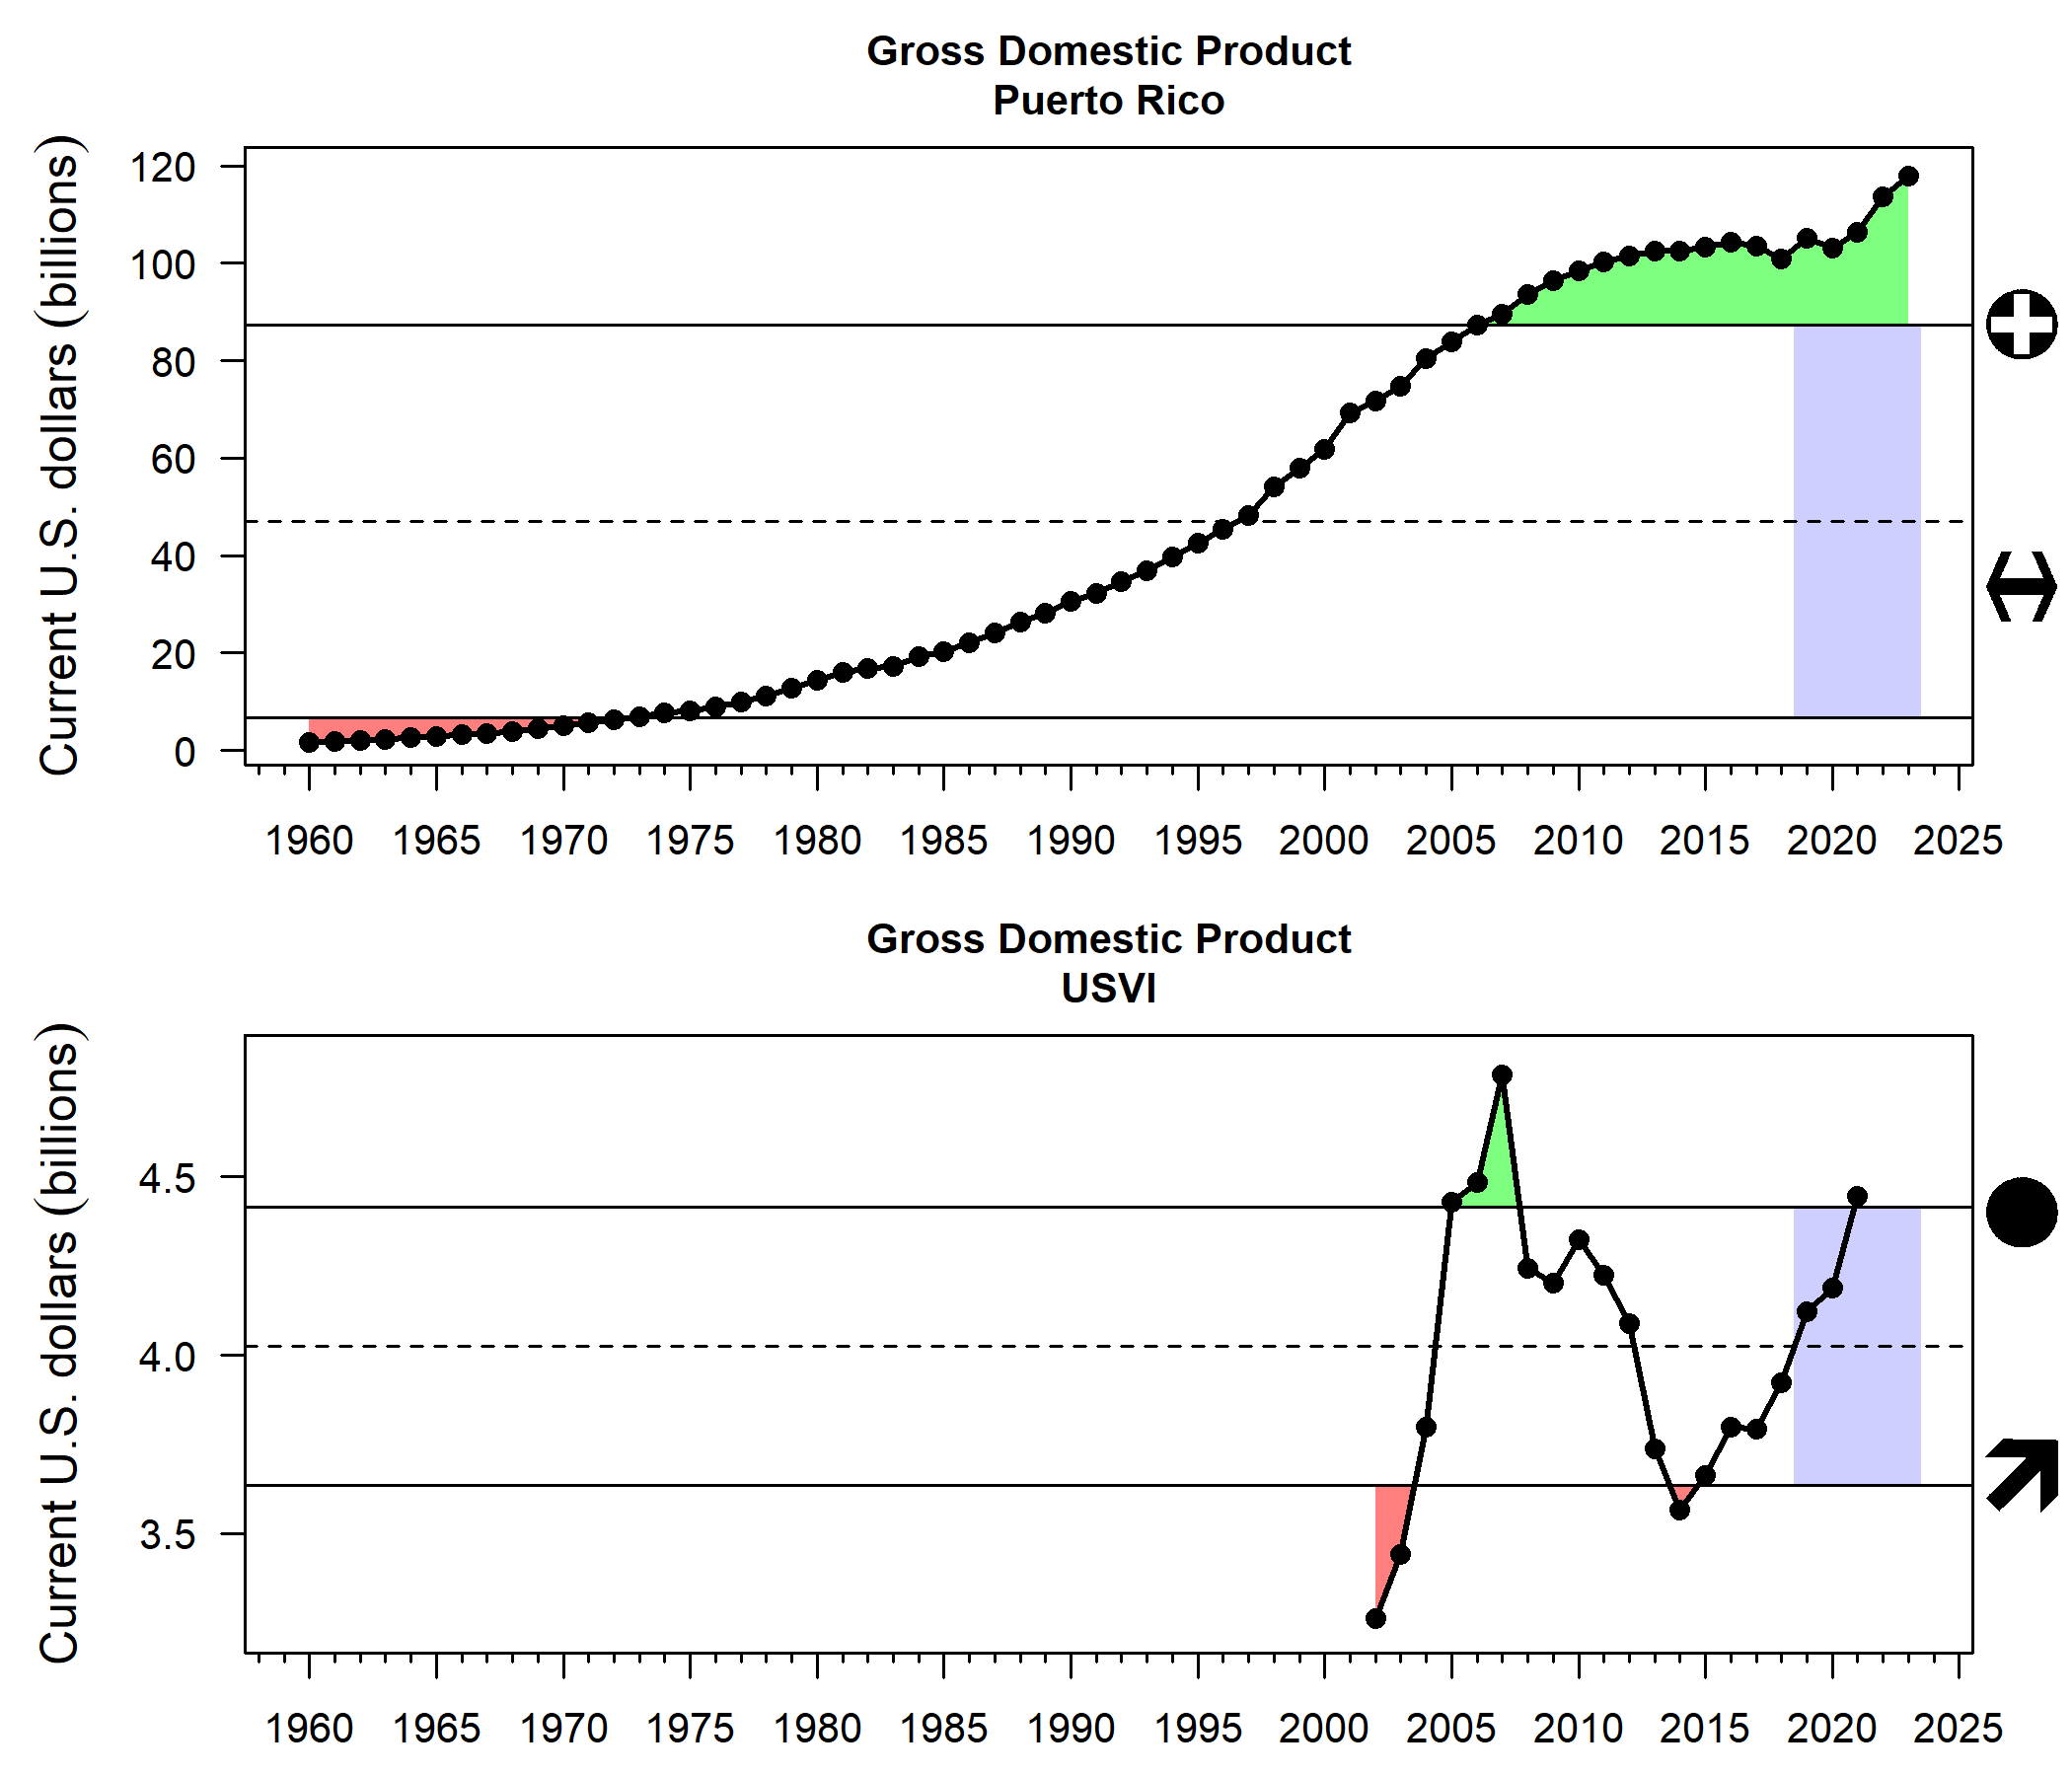
\includegraphics[width=0.75\linewidth,height=\textheight,keepaspectratio]{indicator_plots/GDP_plot_final.png}

}

\caption{\label{fig-GDP}Overall Gross Domestic Product in Puerto Rico
(top) and the USVI (bottom).}

\end{figure}%

GDP can sometimes underestimate the ocean-dependency of the regions'
local island economies; another indicator that is useful is
employment/unemployment rate data, which come from the U.S. Bureau of
Labor Statistics (U. S. Bureau of Labor Statistics 2024) and the U.S.
Employment and Training Administration (U.S. Employment and Training
Administration 2024). Unemployment has shown a declining trend over time
in Puerto Rico and the USVI. In the USVI, there were notable spikes in
the unemployment rate in 2018 and 2020, following major hurricanes Irma
and Maria and the COVID-19 pandemic.

\begin{figure}

\centering{

\pandocbounded{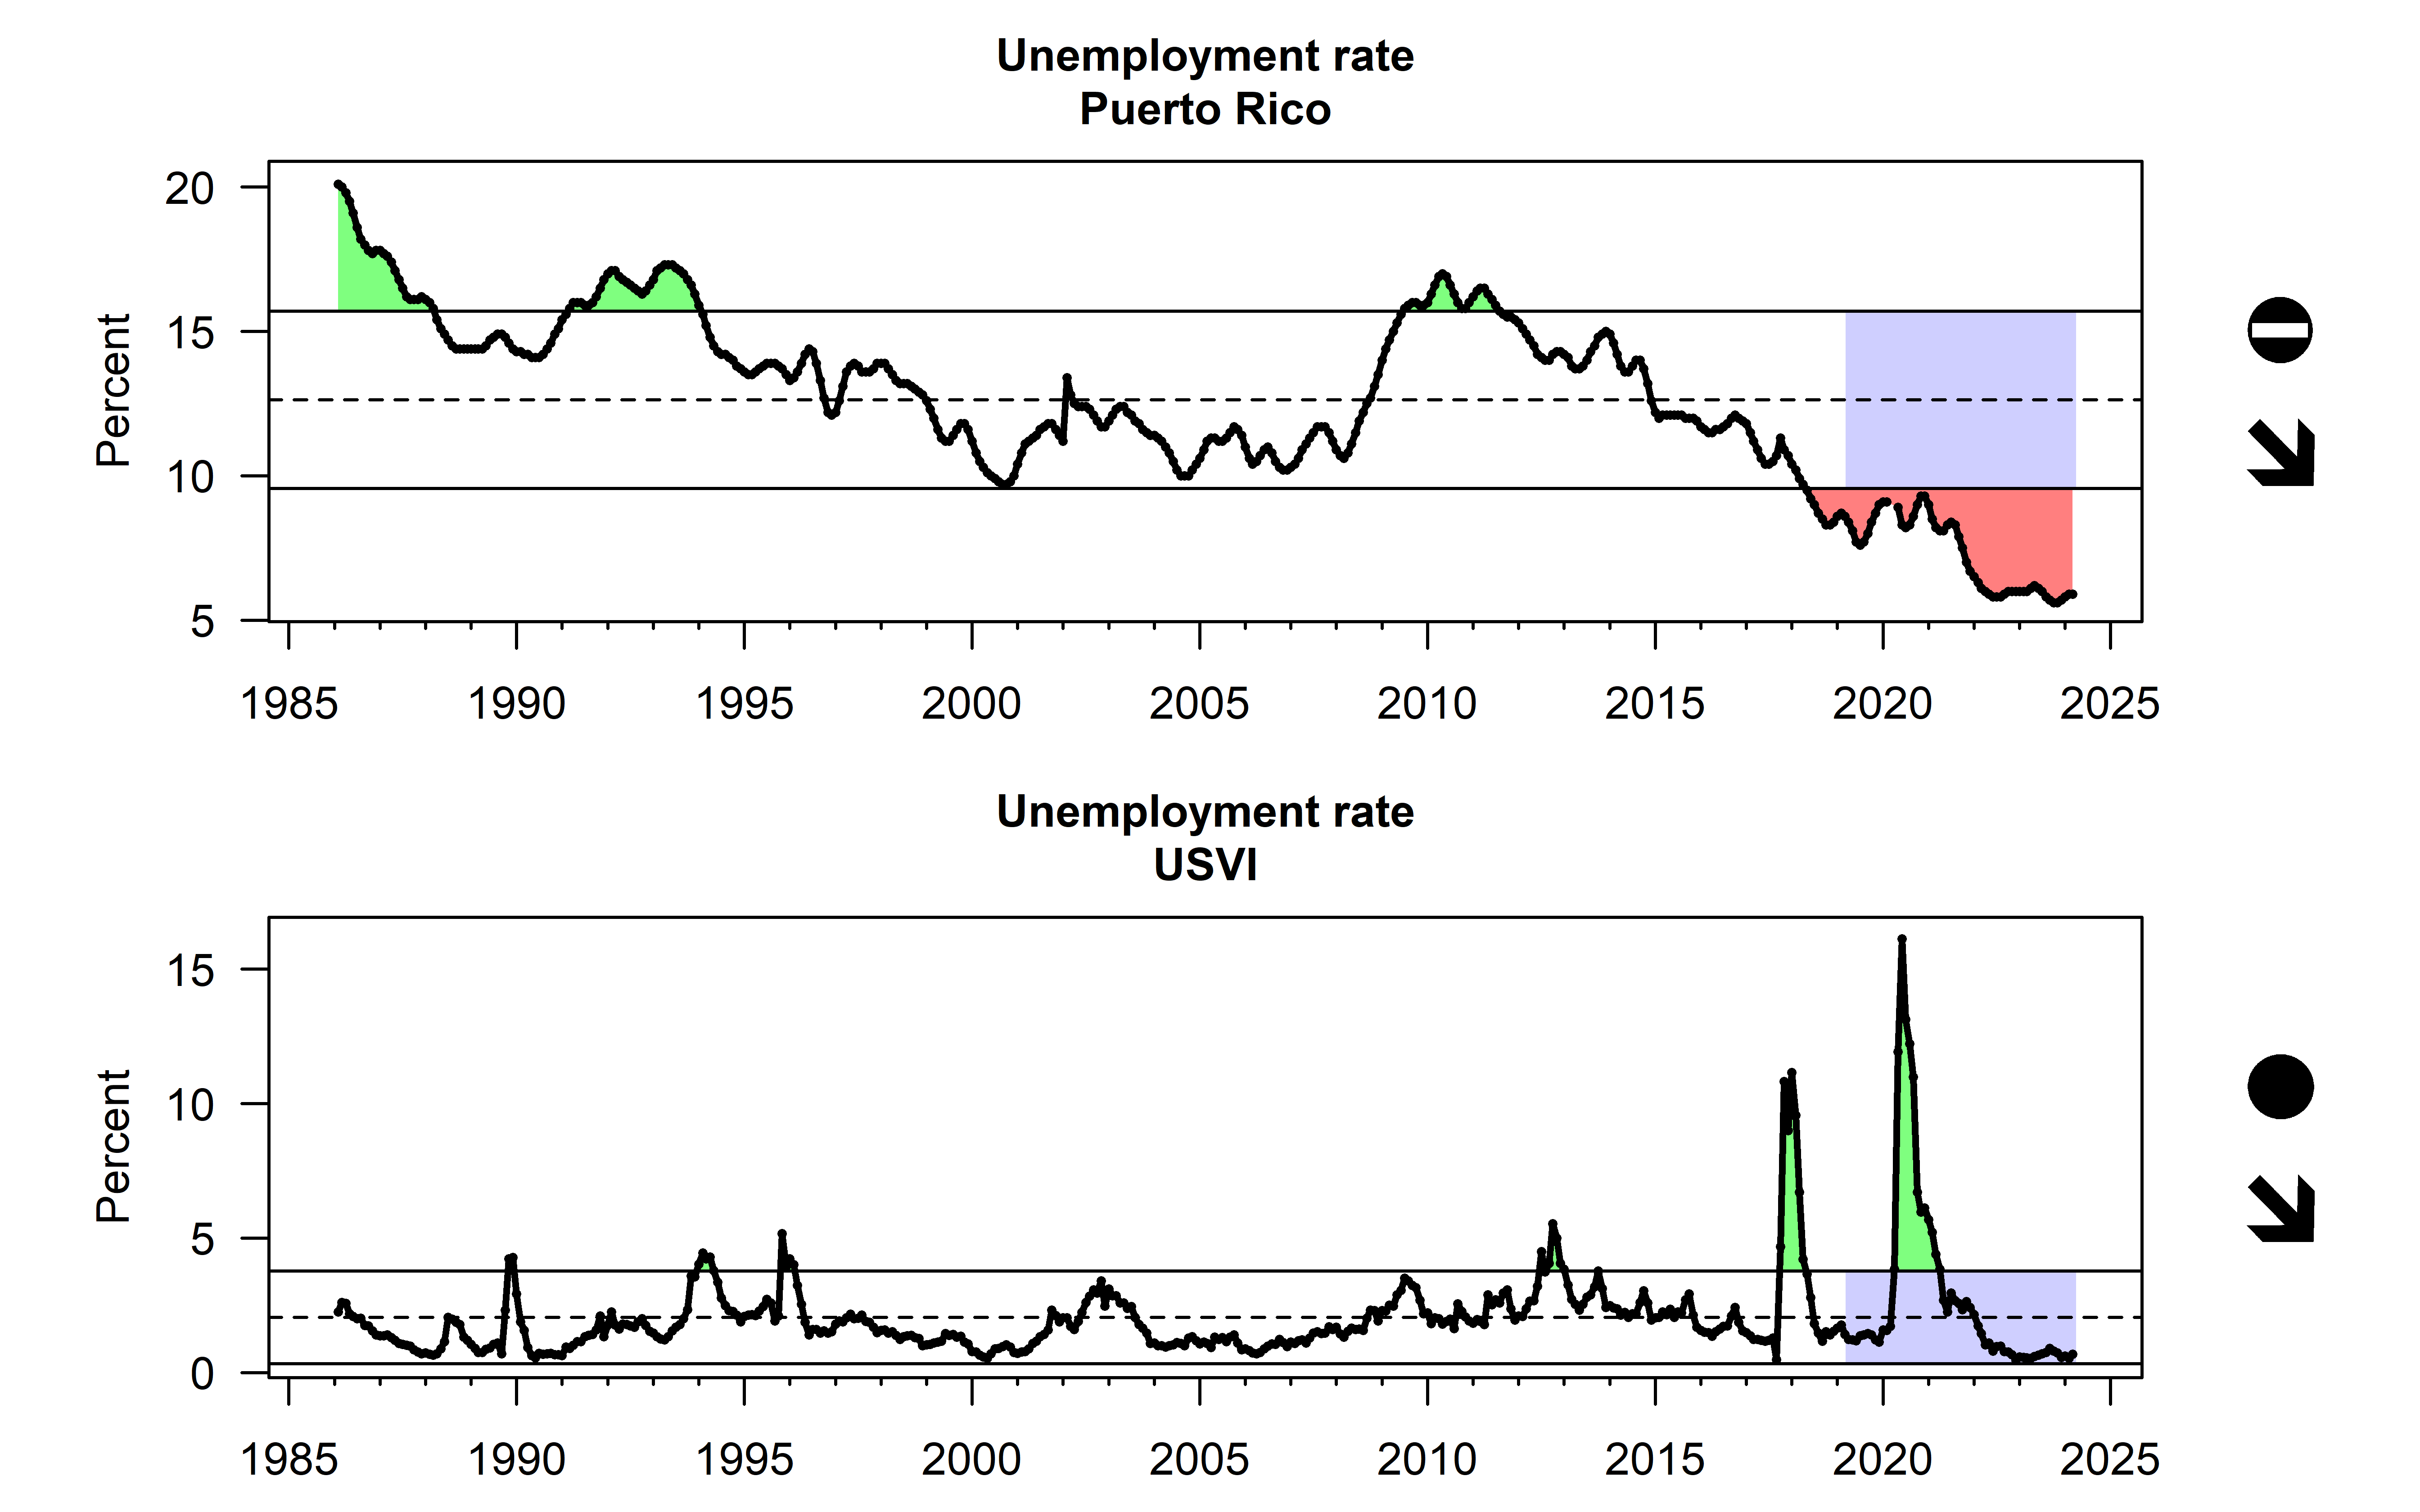
\includegraphics[keepaspectratio]{indicator_plots/unemployment_plot_final.png}}

}

\caption{\label{fig-unemp}Monthly unemployment rate in Puerto Rico (top)
and the USVI (bottom).}

\end{figure}%

\subsection{Ocean economy}\label{ocean-economy}

Due to their unique geography, culture and setting, the islands of
Puerto Rico and the USVI are more reliant on the surrounding ocean and
marine environments than many parts of the continental United States.
Data from the Bureau of Labor Statistics Quarterly Census of Employment
and Wages (\url{https://www.bls.gov/cew/downloadable-data-files.htm})
provide data on the number of establishments, employees, and wages
earned for each county by industry (as defined by NAICS code). These
data underpin the Economics: National Ocean Watch (ENOW) methods created
by NOAA's Office for Coastal Management to track contributions of the
ocean economy to the overall economy. There were significant changes to
the way ocean economy metrics were calculated for the U.S. Territories
in 2016 (Clements, Feliciano, and Colgan 2016), and revised metric data
are only available from 2019-2021 through ENOW. It is therefore
difficult to assess trends over time until additional data are collected
(Figure~\ref{fig-NAICS}).

\begin{figure}

\centering{

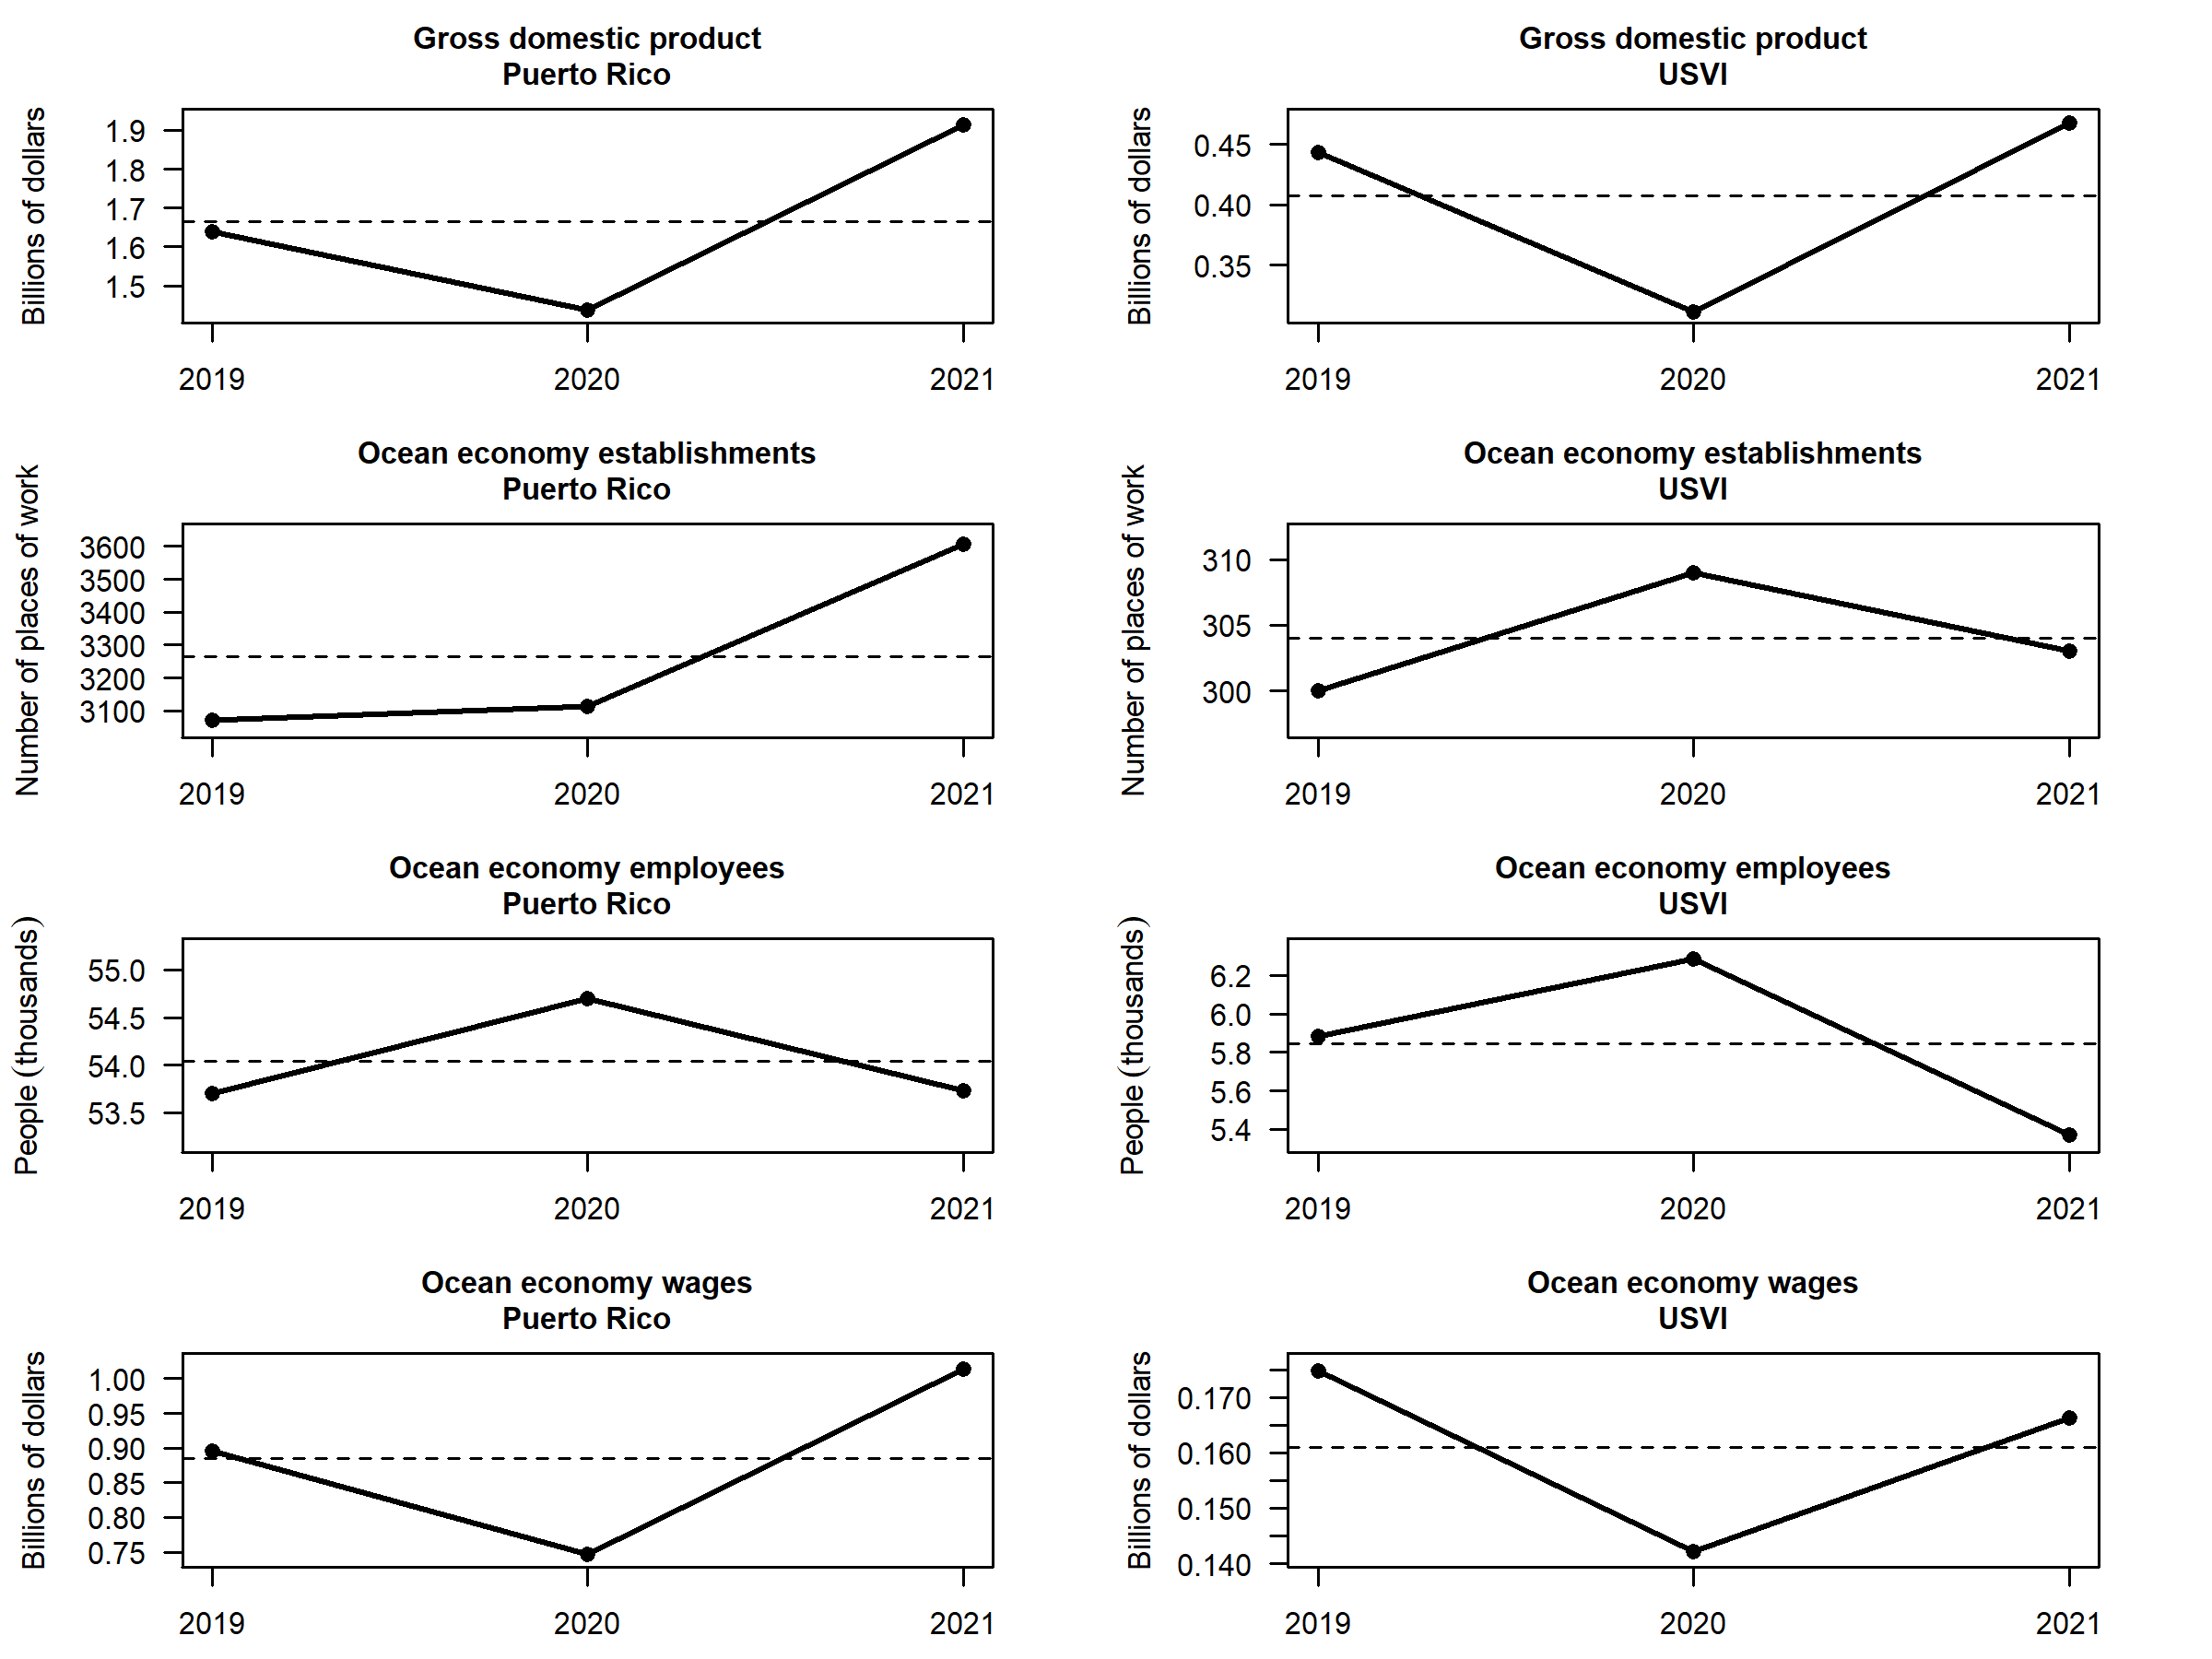
\includegraphics[width=0.75\linewidth,height=\textheight,keepaspectratio]{indicator_plots/oceanNAICS_plot_final.png}

}

\caption{\label{fig-NAICS}Ocean economy GDP, ocean economy
establishments, ocean economy employment, and ocean economy wages (from
top to bottom), for Puerto Rico (left column) and the USVI (right
column).}

\end{figure}%

\section{Equity}\label{equity}

\subsection{Commercial revenue
distribution}\label{commercial-revenue-distribution}

Equality in the distribution of revenues across the fishery can be
represented by the Gini index which is a value ranging from zero to one,
with zero representing perfect equality (revenues distributed equally
among all participants) and a value of one representing maximum
inequality (all revenues going to a single individual, Gini 1936). The
Gini index was calculated based on reported revenues from the Caribbean
Commercial Landings database, as they are distributed across the
individual vessel or fisher permits (Figure~\ref{fig-gini}). Overall,
the Gini index values suggest that consolidation across U.S. Caribbean
fisheries is high compared to other U.S. regions (Brinson and Thunberg
2016), though this may be an artifact of reporting if more experienced
fishermen are more consistent in their reporting. In St.~Thomas and
St.~John, the index shows a gradual increase throughout the time period,
while there is no particular trend apparent in Puerto Rico and
St.~Croix. There are spikes in inequality in Puerto Rico in 2018 and in
St.~Croix in 2017-2018 which may be related to fishing industry impacts
from hurricanes.

\begin{figure}

\centering{

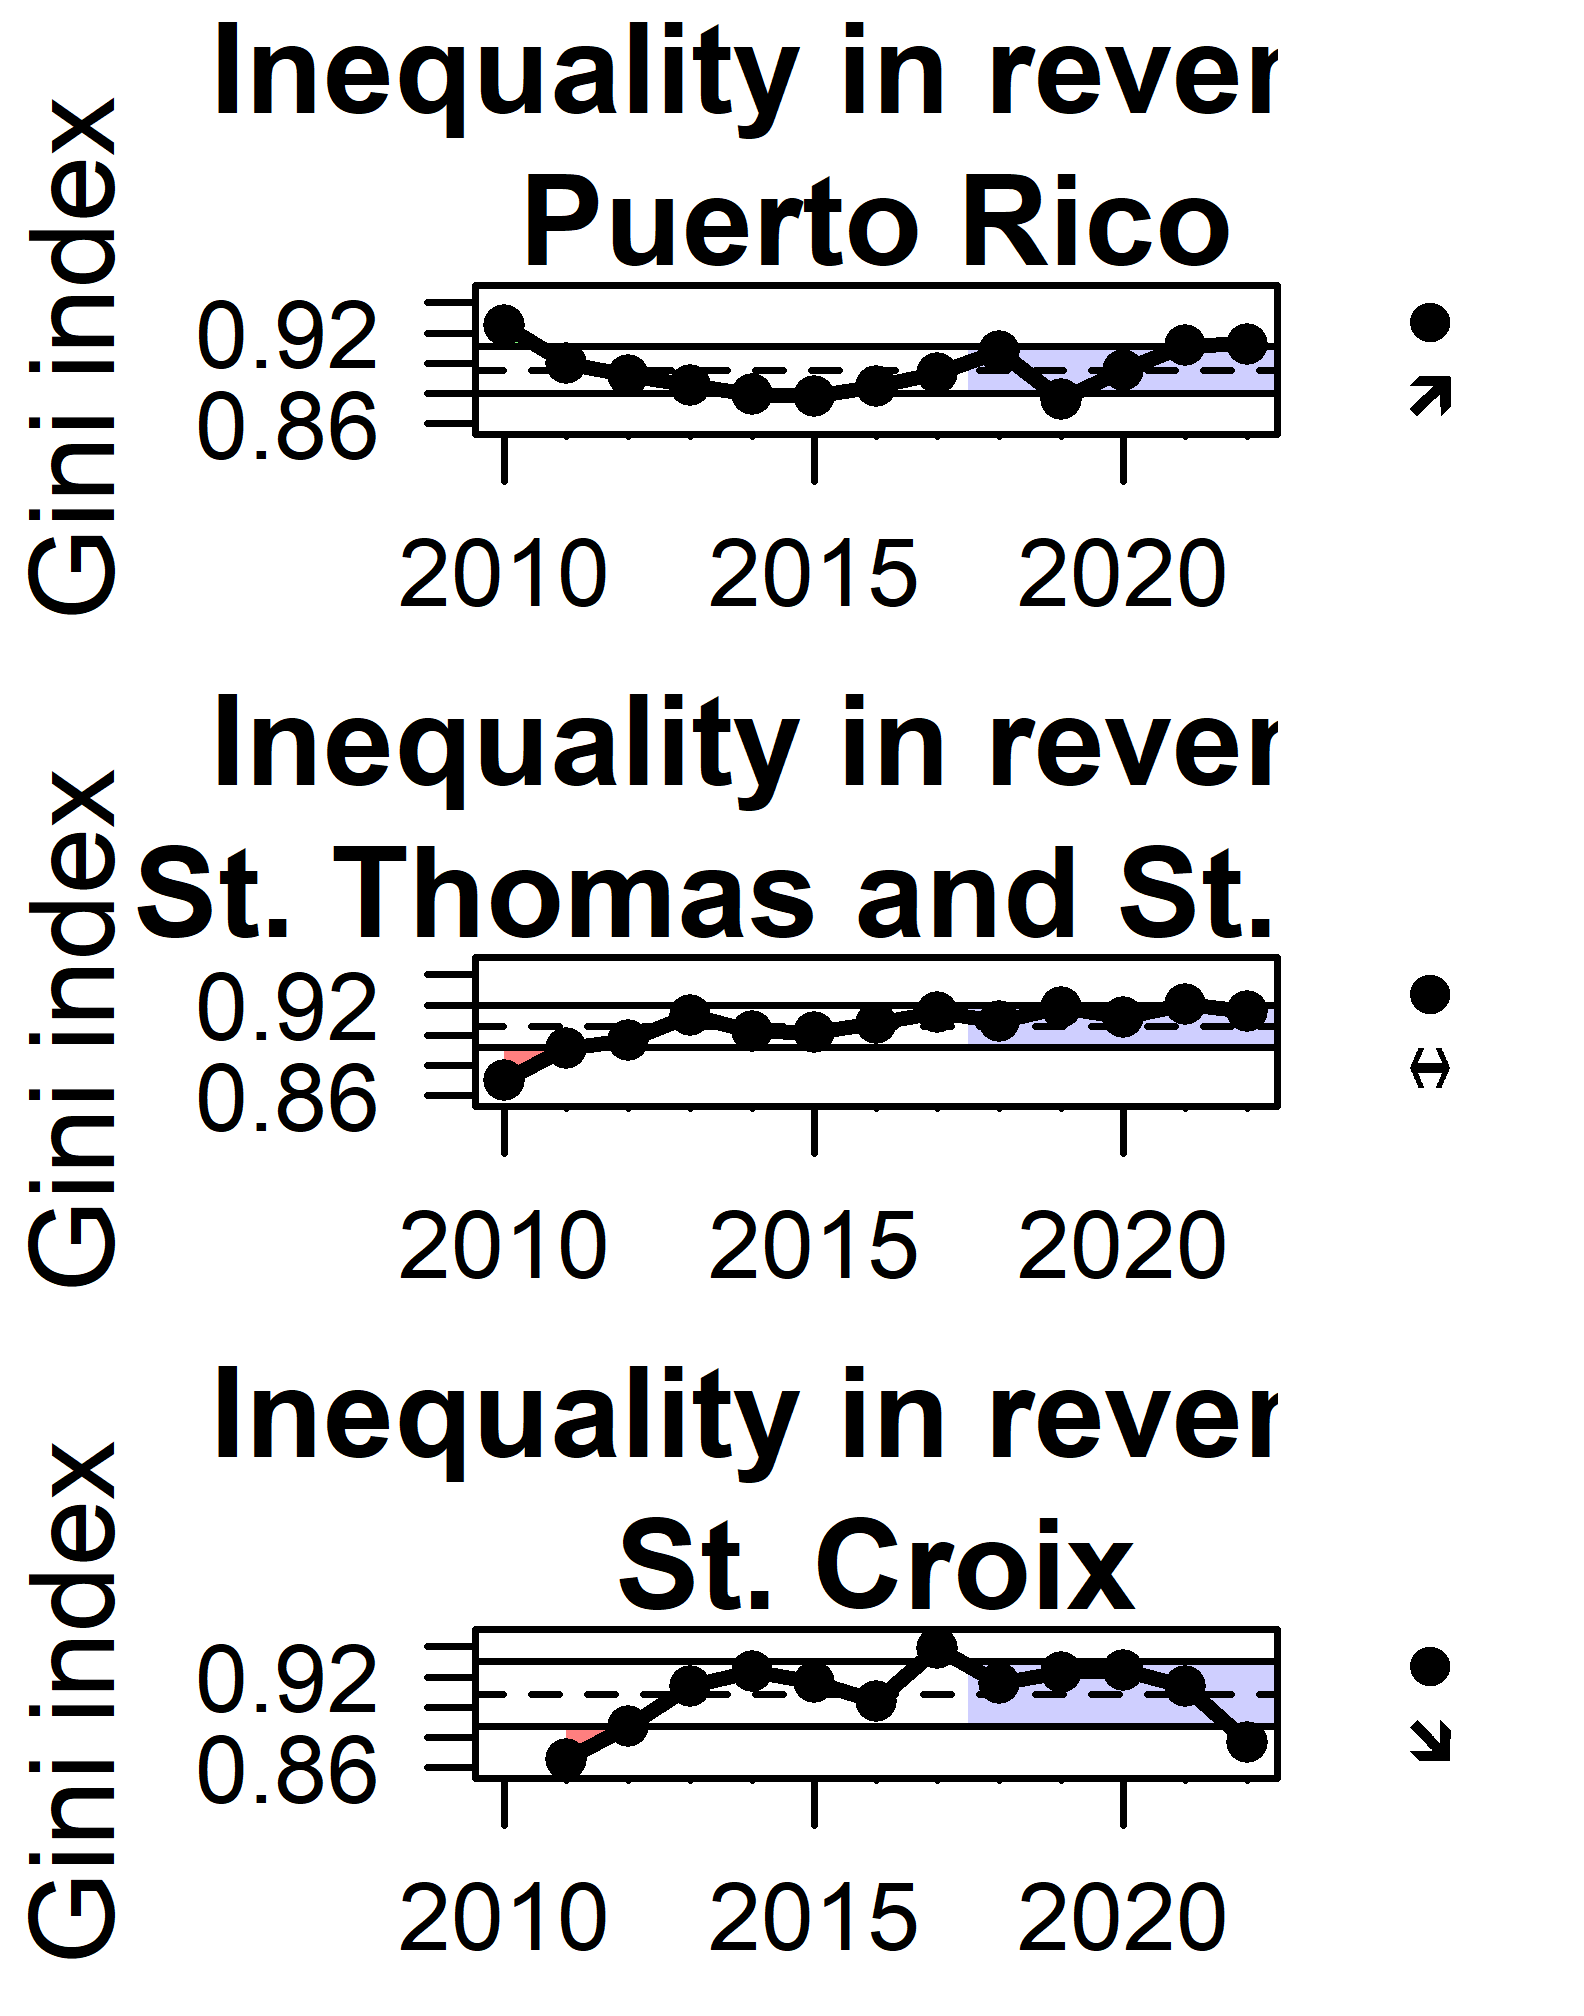
\includegraphics[width=0.75\linewidth,height=\textheight,keepaspectratio]{indicator_plots/gini_plot_final.png}

}

\caption{\label{fig-gini}Equality in the distribution of revenues across
the commercial fishery Puerto Rico (top), St.~Thomas and St.~John
(middle) and St.~Croix (bottom), as represented by the Gini index. Note
that the years in the USVI are fishing years (July 1st to June 30th of
the following year).}

\end{figure}%

\section{Engagement and
participation}\label{engagement-and-participation}

\subsection{Recreational landings}\label{recreational-landings}

Recreational catch and effort is a major data gap in the U.S. Caribbean.
The Marine Recreational Information Program collected complete years of
data in Puerto Rico up until 2016, and in the USVI there are no regular
monitoring programs. The Sea Around Us database estimates reported
catches based on imputations and assumptions (Pauly and Zeller 2015). In
Puerto Rico, catch was reconstructed by supplementing the MRIP survey
with a variety of other studies conducted at various points in time. In
the USVI, catch was reconstructed based on a telephone survey conducted
by the USVI Division of Fish and Wildlife to estimate resident
participation and catch rates, and adding a conservative estimate of
tourist catches. These reconstructed estimates suggest that recreational
catch has been declining over the last several decades in Puerto Rico,
whereas catch has increased over the same period in the USVI
(Figure~\ref{fig-reccatch}).

\begin{figure}

\centering{

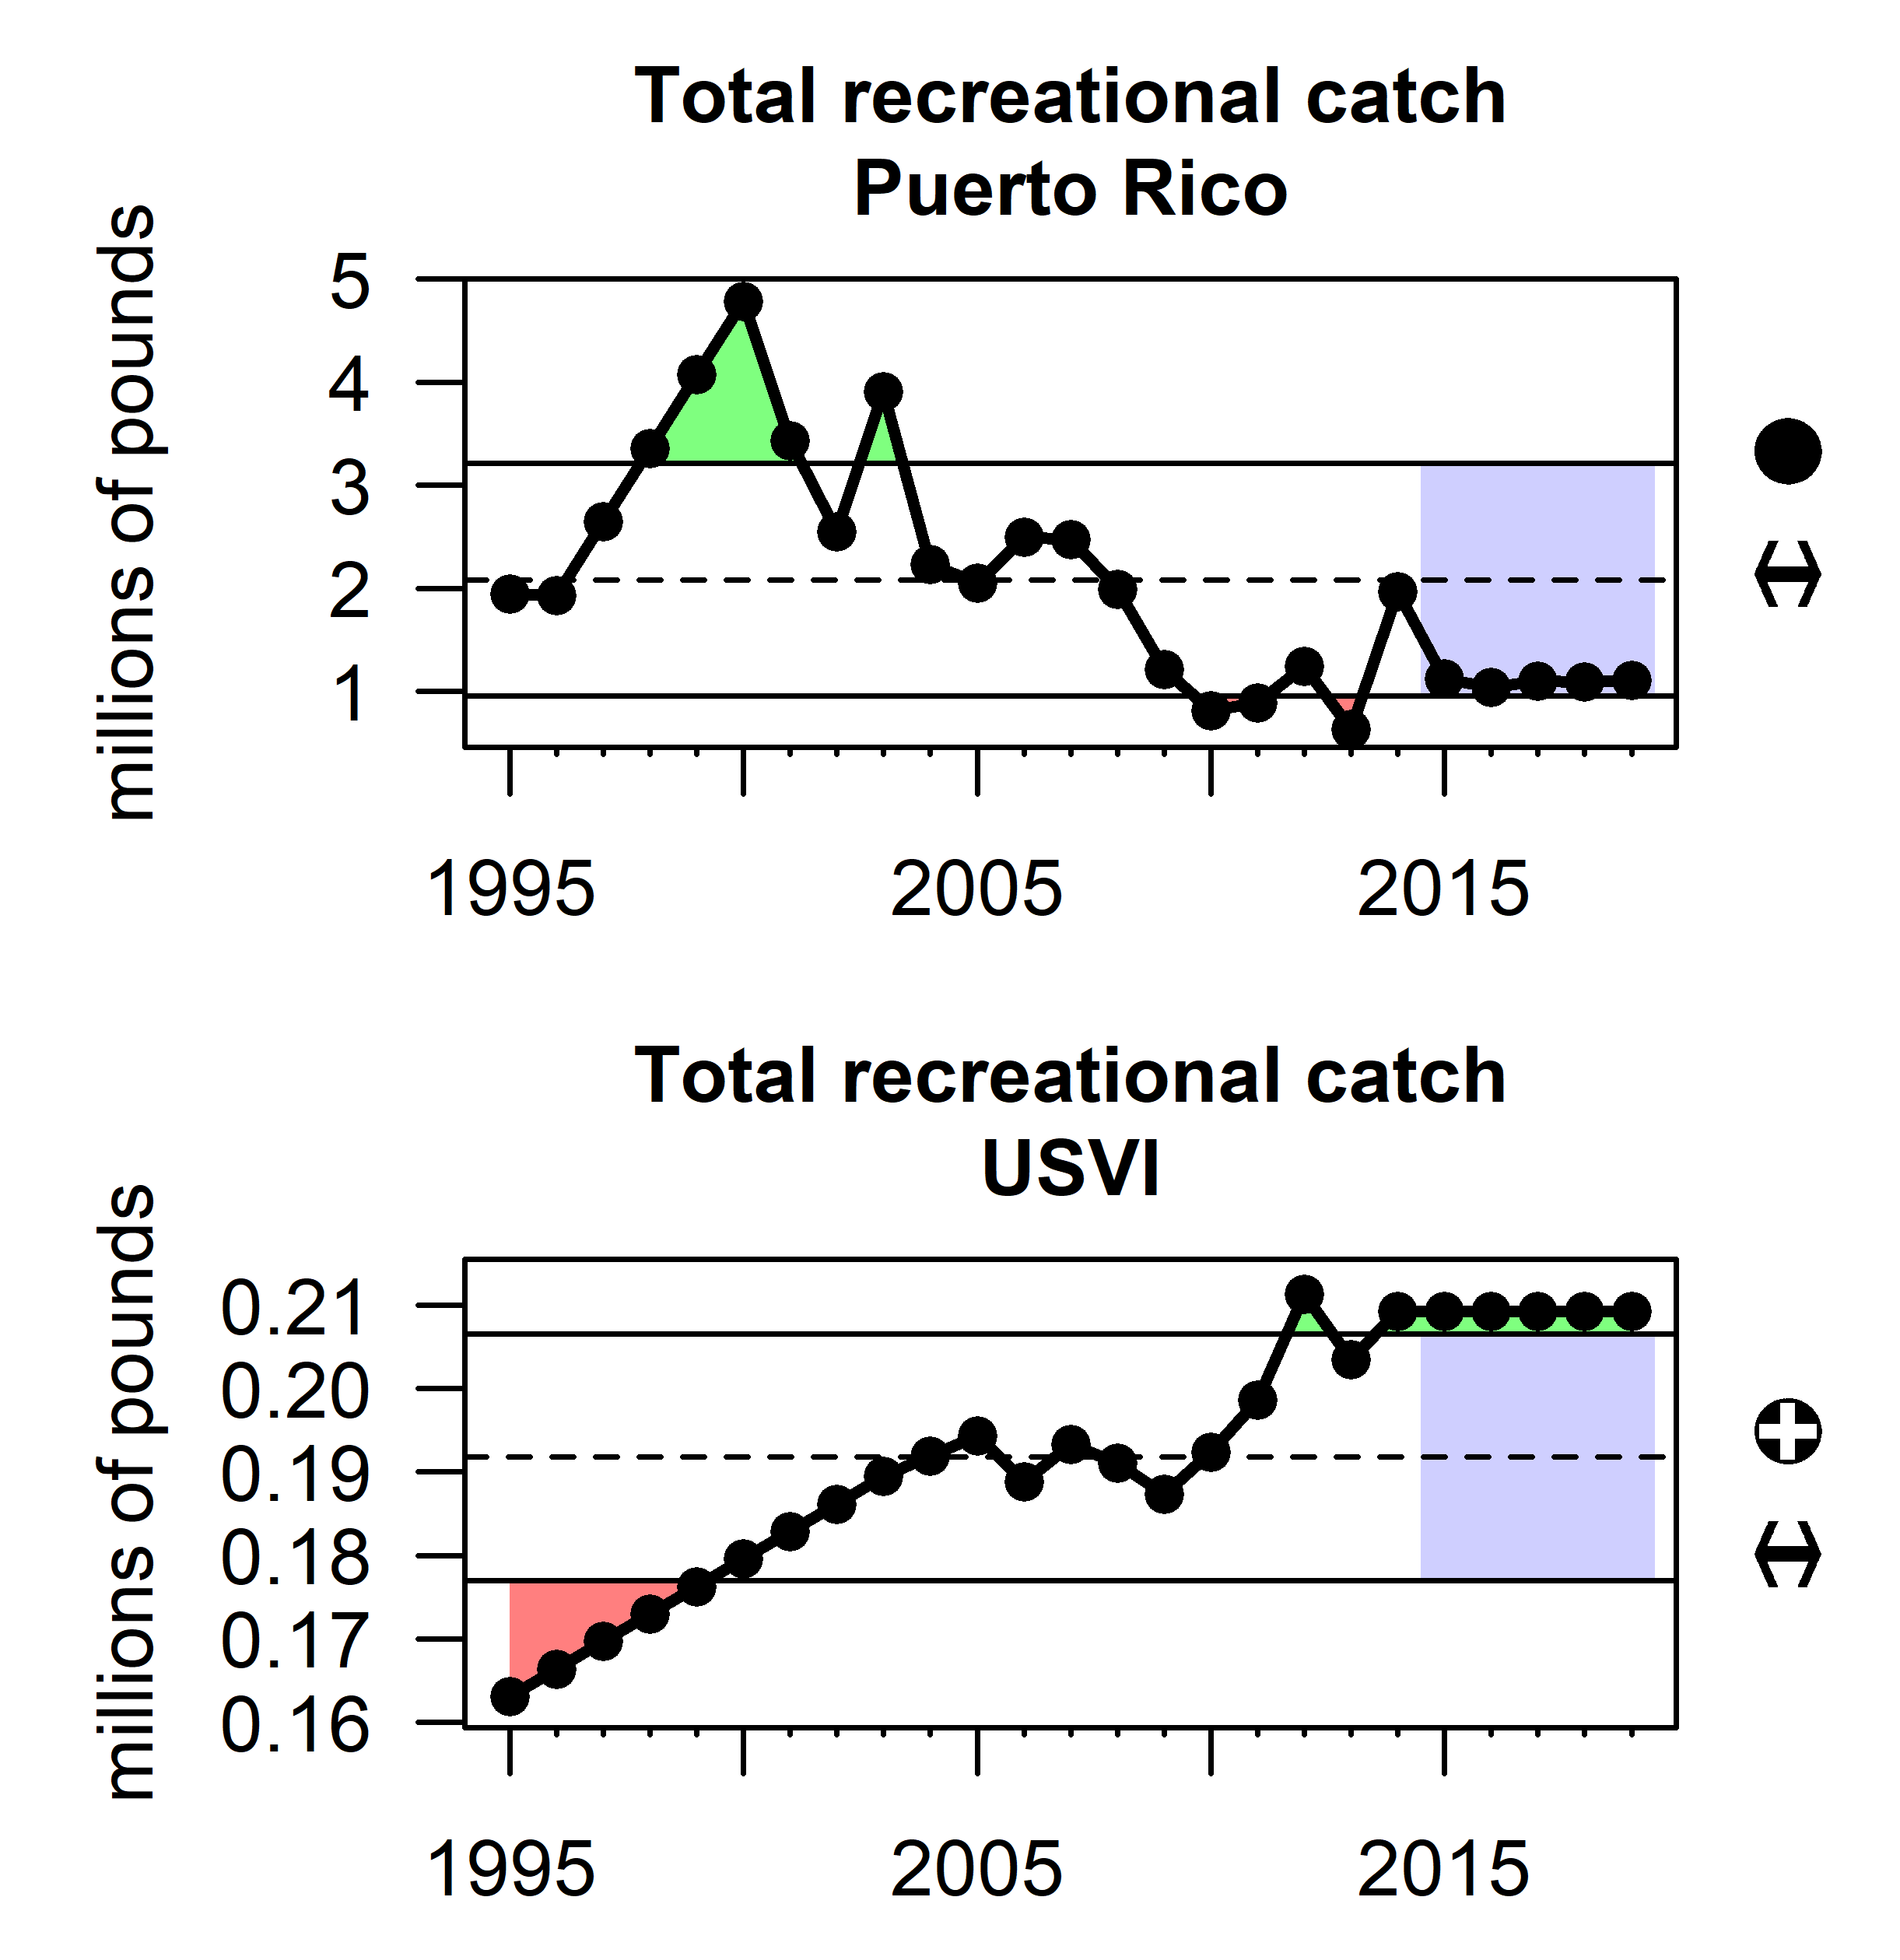
\includegraphics[width=0.75\linewidth,height=\textheight,keepaspectratio]{indicator_plots/total_rec_catch_plot_final.png}

}

\caption{\label{fig-reccatch}Total recreational catch in millions of
pounds as estimated by the Sea Around Us database for Puerto Rico (top)
and the USVI (bottom).}

\end{figure}%

\subsection{Commercial fishing engagement and
reliance}\label{commercial-fishing-engagement-and-reliance}

Fishing engagement and reliance indices measure the importance and level
of dependence on commercial or recreational fishing for coastal
communities (NOAA Fisheries 2024). Commercial fishing engagement
measures the presence of commercial fishing through fishing activity as
shown through permits, fish dealers, and vessel landings. A high rank
indicates more engagement. Commercial fishing reliance measures the
presence of commercial fishing in relation to the population size of a
community through fishing activity. A high rank indicates more reliance.
Coastal communities on the west and east coasts of Puerto Rico, the
north side of St.~Thomas, and the southwest of St.~Croix had
particularly high commercial engagement and reliance for 2016--2020
(Figure~\ref{fig-PRengage}, Figure~\ref{fig-PRreliance},
Figure~\ref{fig-USVIengage}).

\begin{figure}

\centering{

\pandocbounded{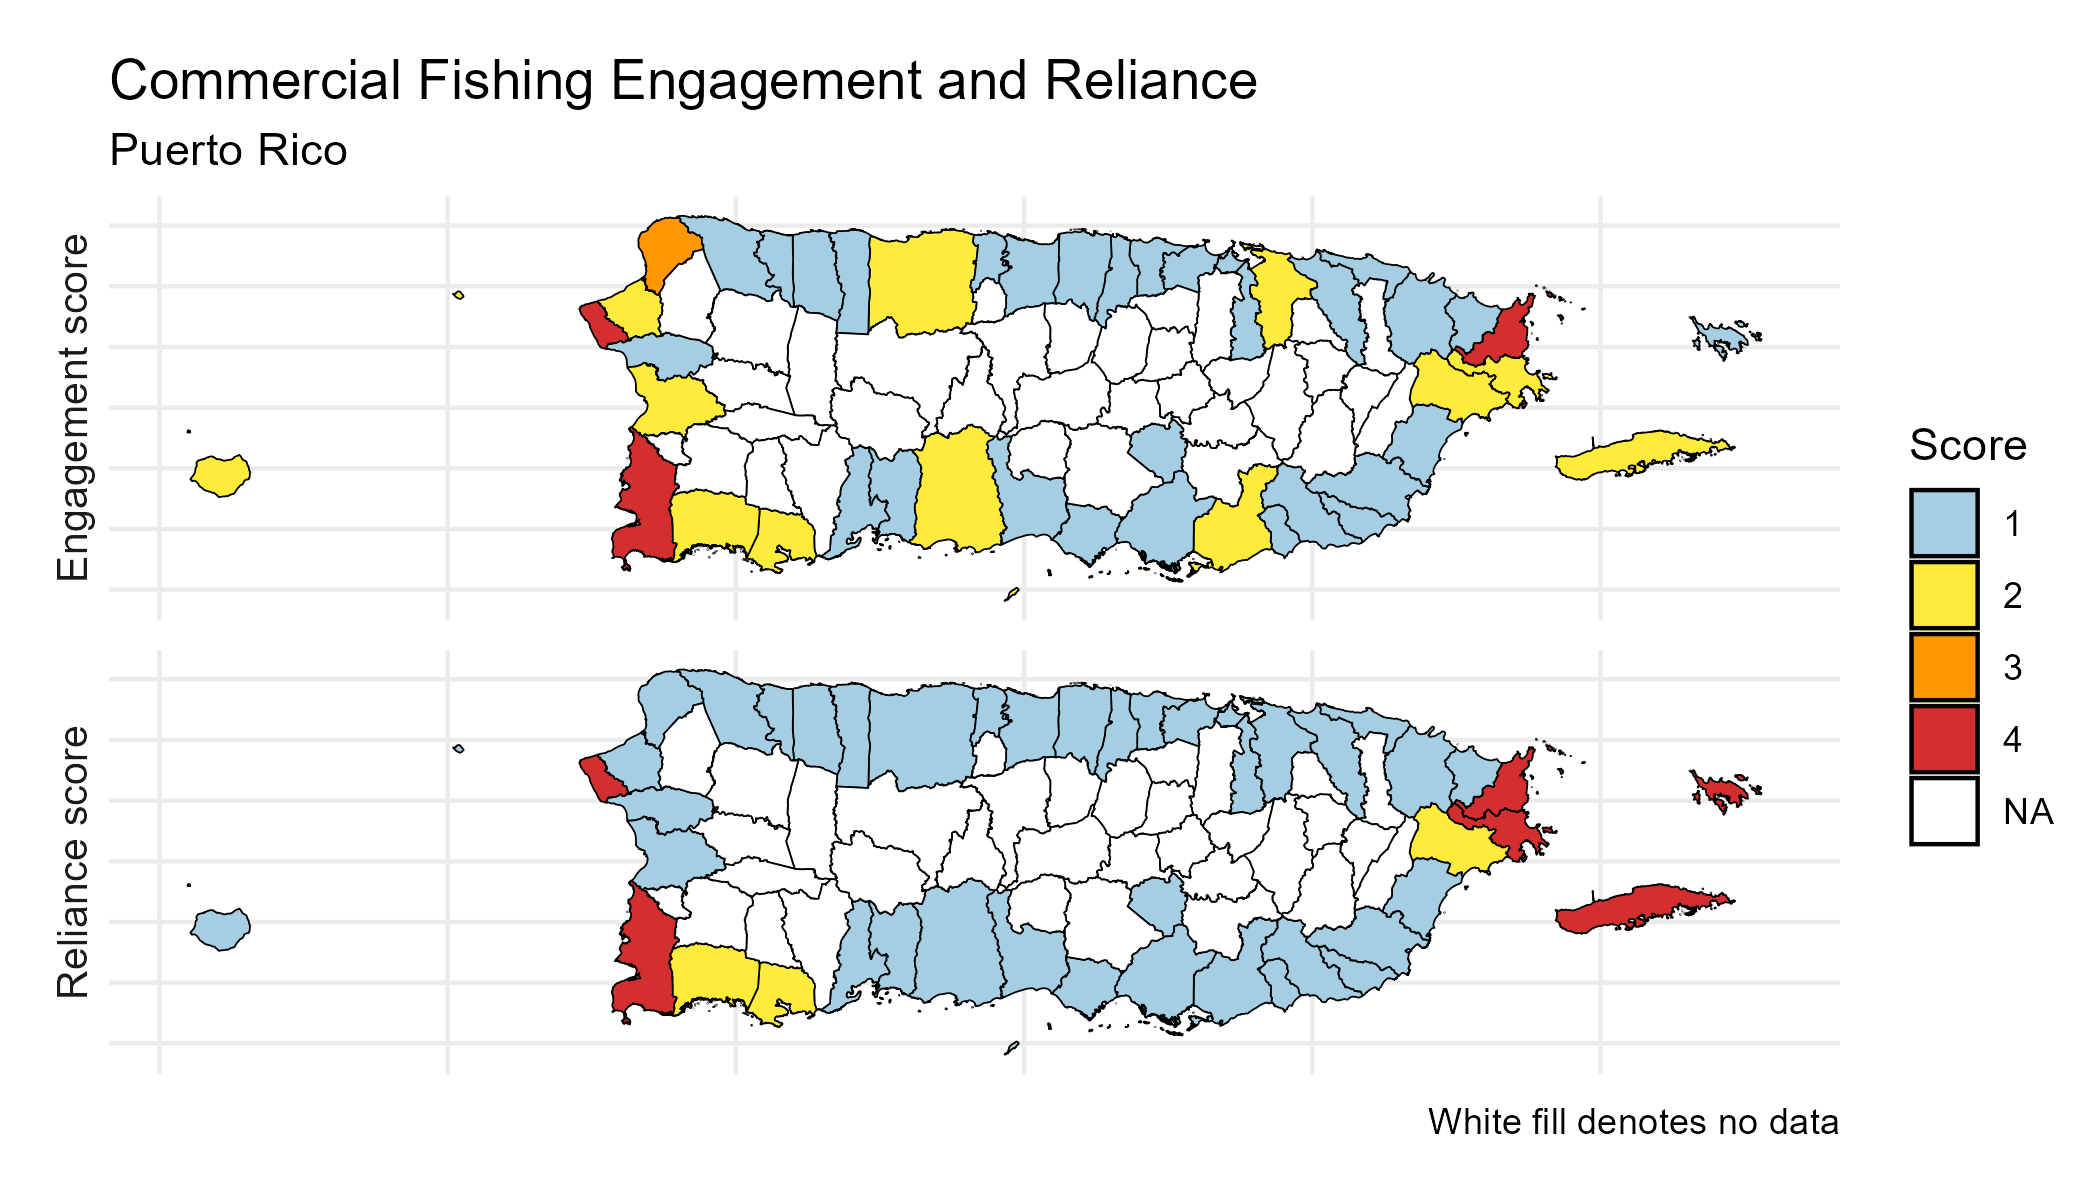
\includegraphics[keepaspectratio]{indicator_plots/CSVI_plots/PR_engrel_maps.png}}

}

\caption{\label{fig-PRengage}Commercial fishing engagement and reliance
in Puerto Rico based on NOAA Fisheries Databases: commercial landings
5-year average for 2016--2020 and permit numbers; and Census data:
Population by municipality/sub-district}

\end{figure}%

\begin{figure}

\centering{

\pandocbounded{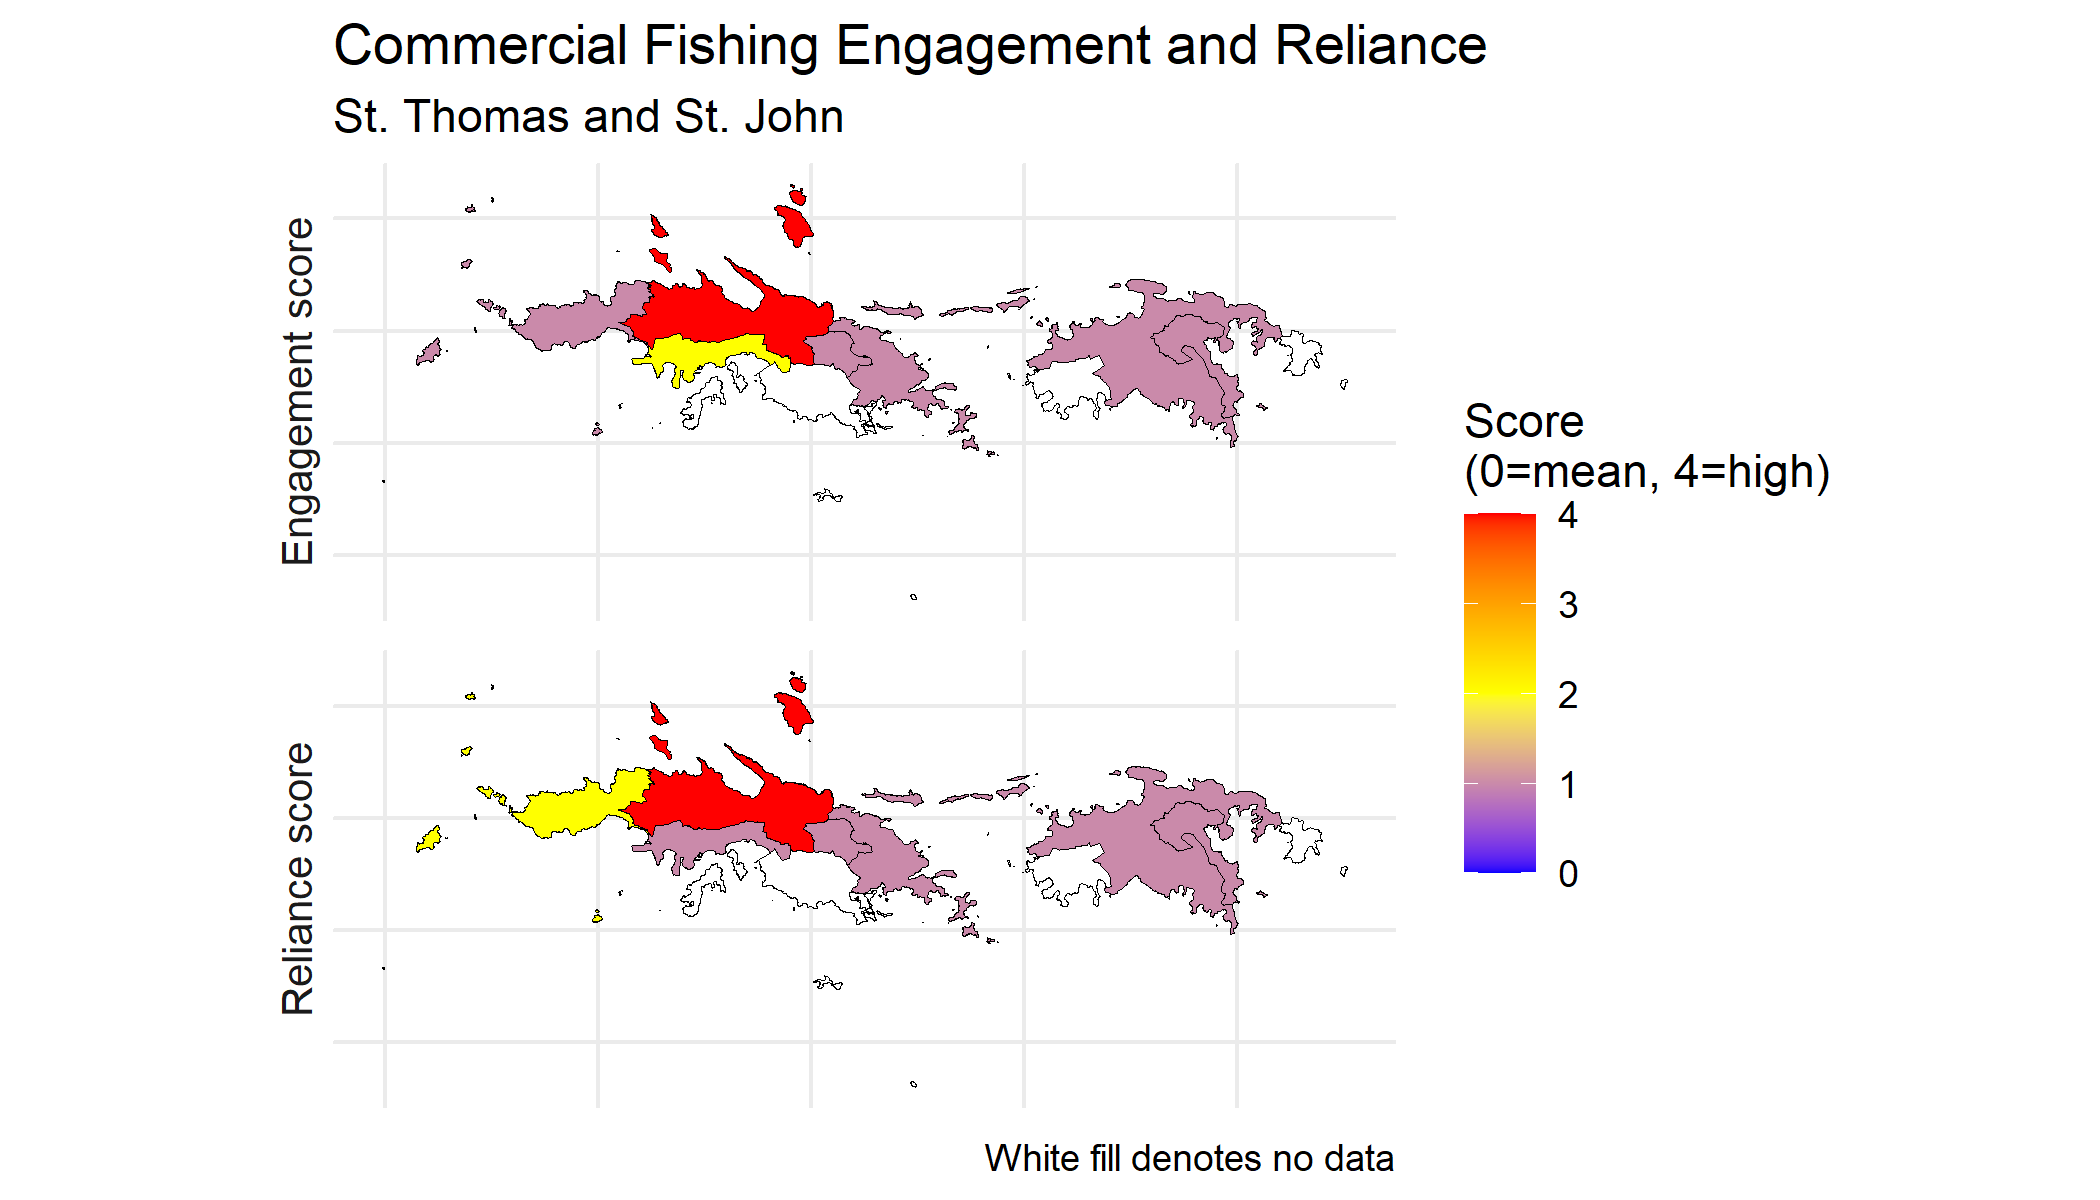
\includegraphics[keepaspectratio]{indicator_plots/CSVI_plots/STSJ_engrel_maps.png}}

}

\caption{\label{fig-PRreliance}Commercial fishing engagement and
reliance in St.~Thomas and St.~John based on NOAA Fisheries Databases:
Commercial landings 5-year average for 2016--2020 and permit numbers;
and Census data: Population by municipality/sub-district.}

\end{figure}%

\begin{figure}

\centering{

\pandocbounded{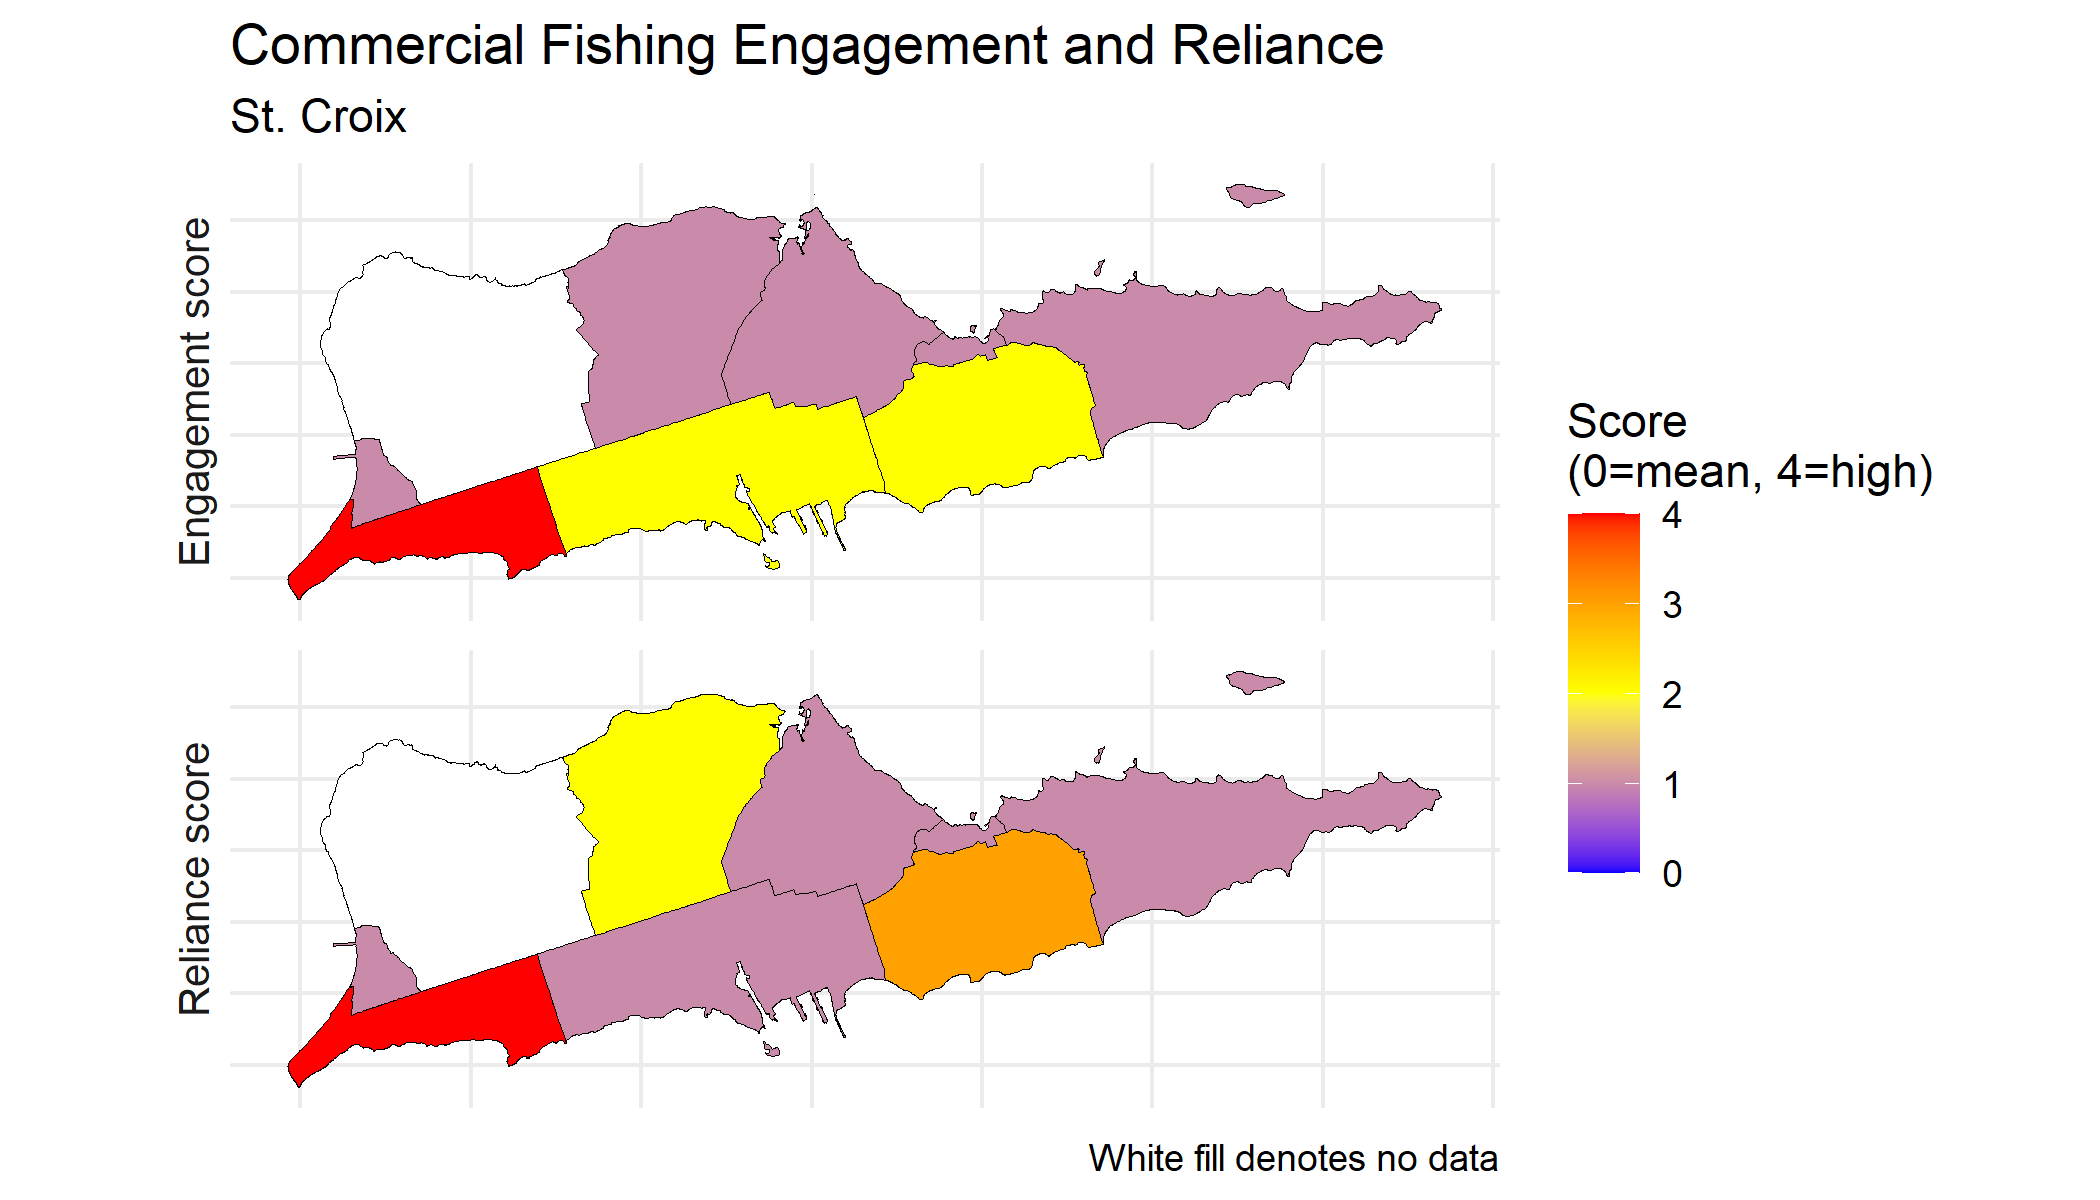
\includegraphics[keepaspectratio]{indicator_plots/CSVI_plots/STX_engrel_maps.png}}

}

\caption{\label{fig-USVIengage}Commercial fishing engagement and
reliance in St.~Croix based on NOAA Fisheries Databases: commercial
landings 5-year average for 2016--2020 and permit numbers; and Census
data: Population by municipality/sub-district}

\end{figure}%

\section{Bycatch reduction}\label{bycatch-reduction}

\subsection{Changes in gear type}\label{changes-in-gear-type}

Data on bycatch in the U.S. Caribbean are generally lacking; target
species and bycatch are not differentiated on most logbook forms and the
region has minimal observer program coverage (and only on the pelagic
longline fleet). The selectivity of gear can be considered as some gear
types are highly selective (e.g.~spearfishing and diving) while other
gear types capture a wide range of target and non-target species. We
calculated the proportion of non-selective gear (traps and nets) from
the Caribbean Commercial Landings database as a proxy for bycatch in the
fisheries. Overall the use of these gear types is decreasing in Puerto
Rico and St.~Croix while it is increasing in St.~Thomas and St.~John
(Figure~\ref{fig-bycatch}).

\begin{figure}

\centering{

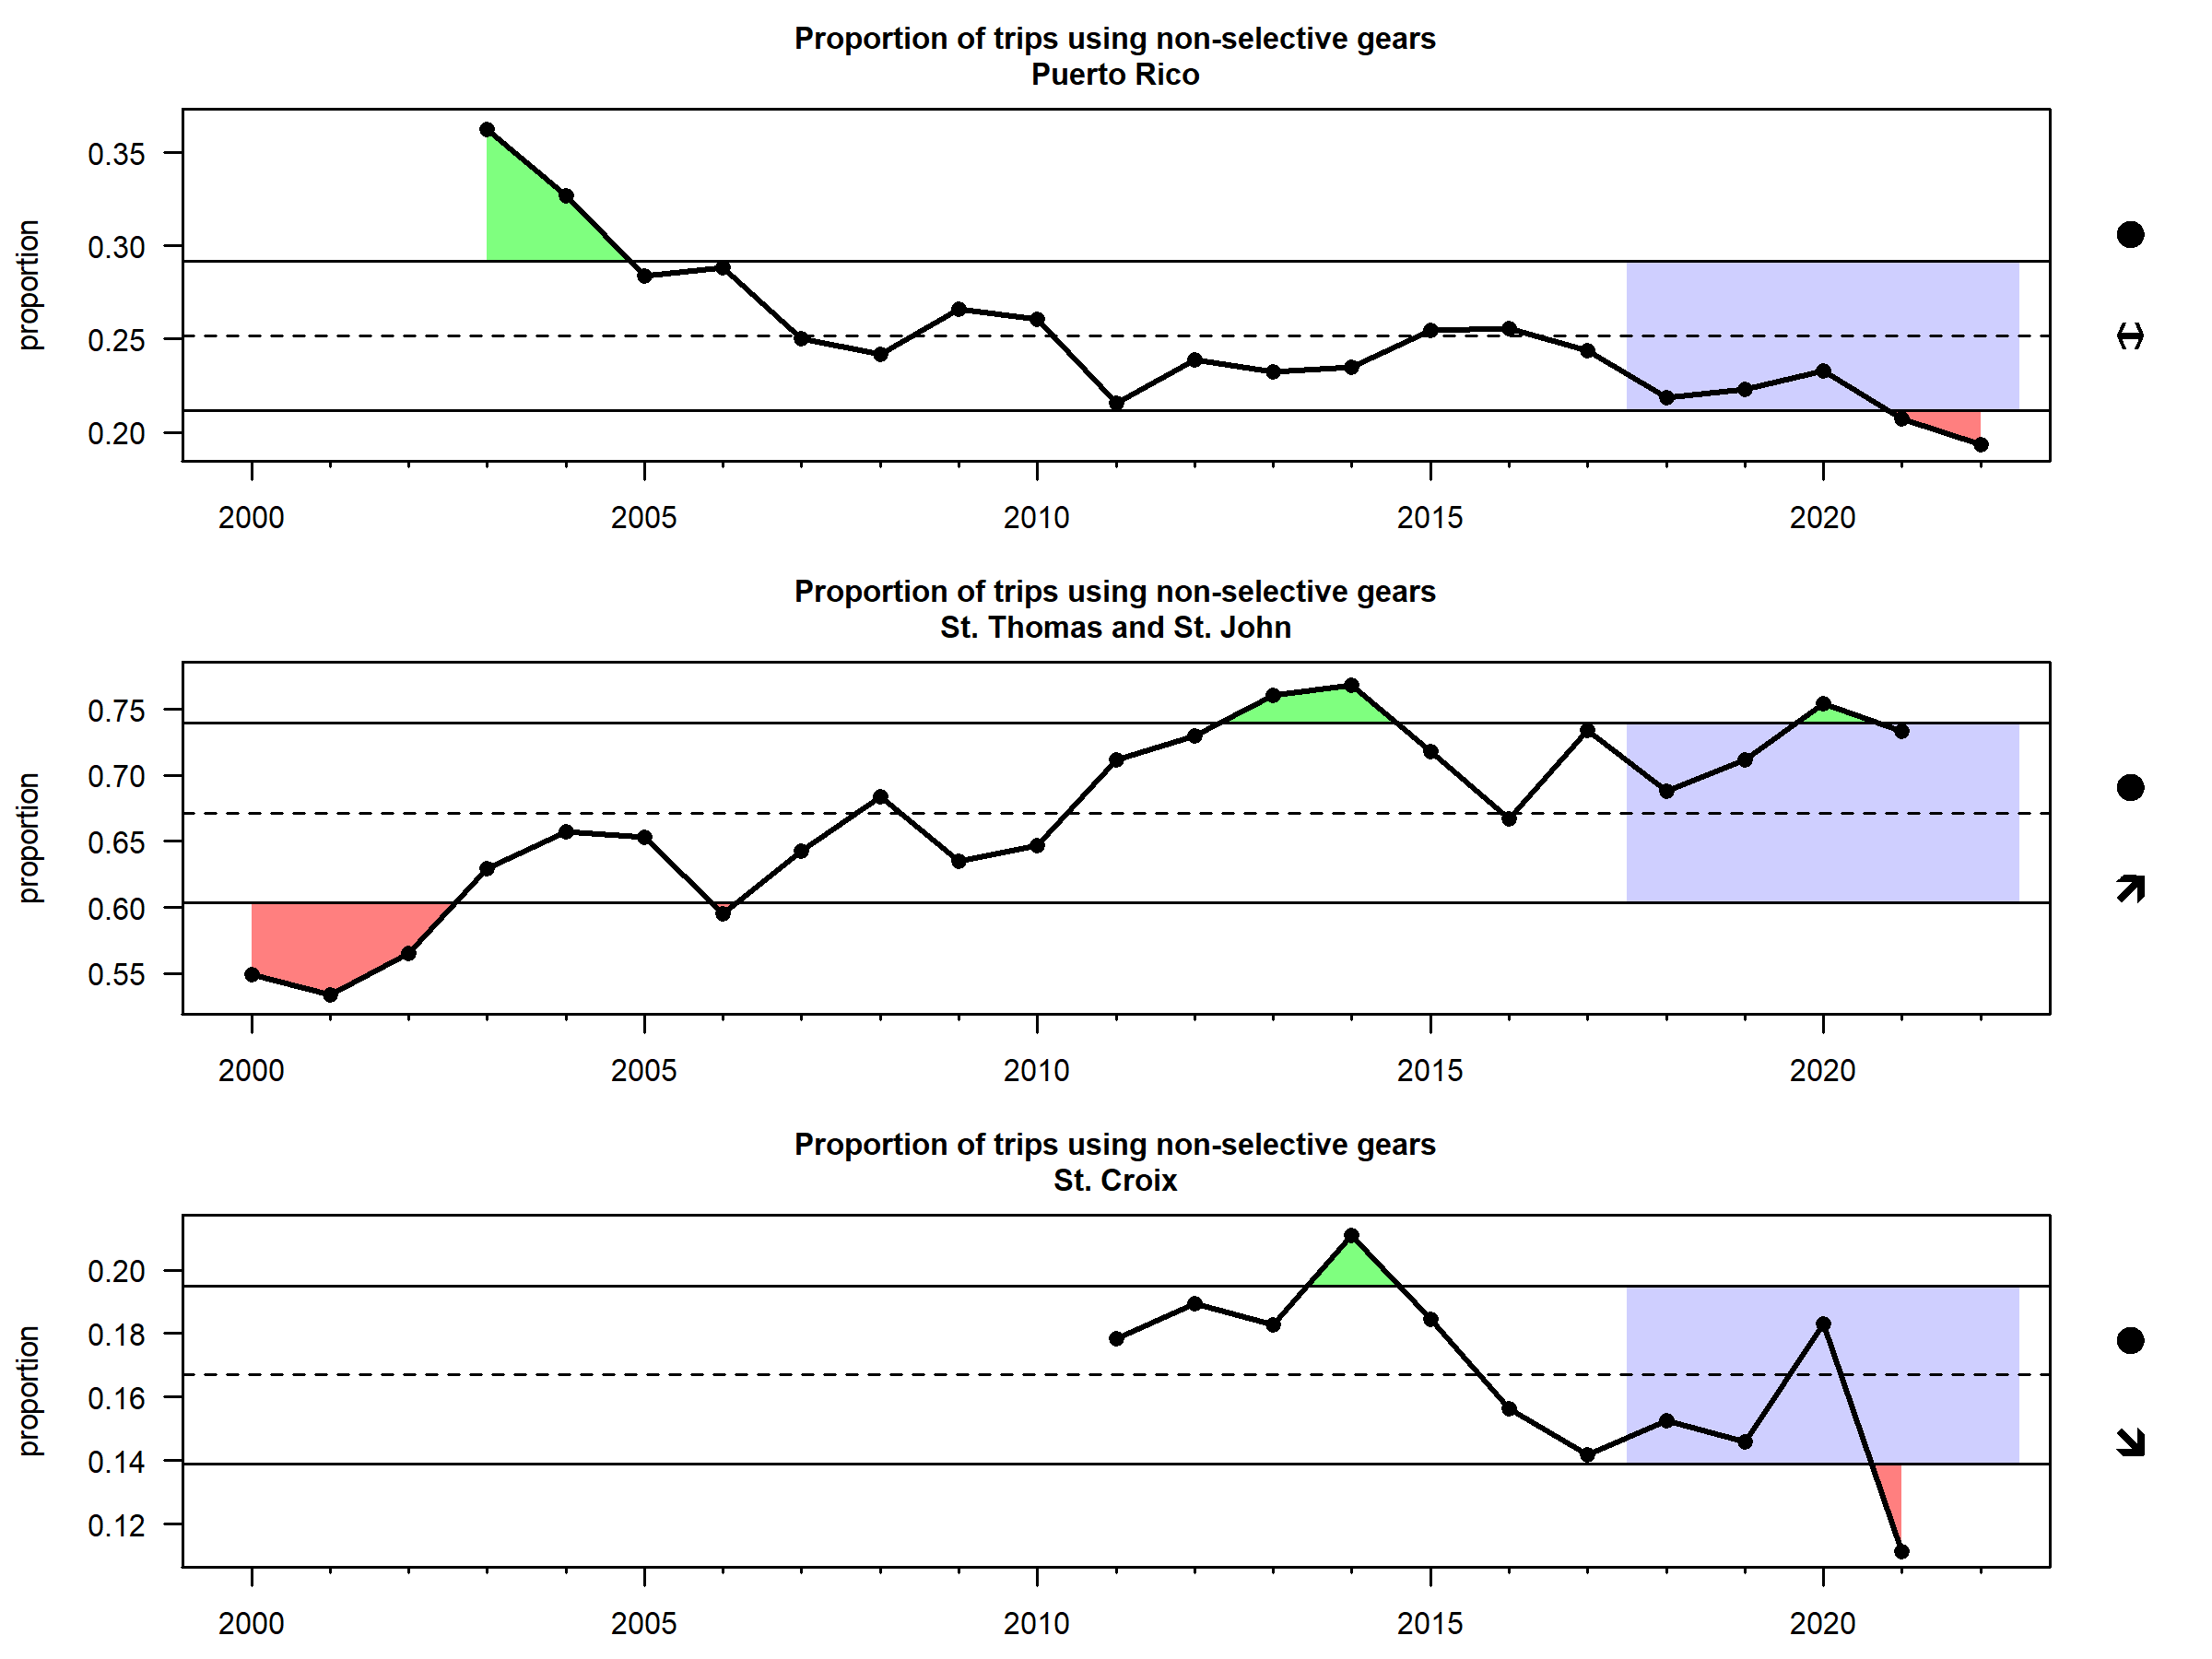
\includegraphics[width=0.75\linewidth,height=\textheight,keepaspectratio]{indicator_plots/prop_trips_bycatch_plot_final.png}

}

\caption{\label{fig-bycatch}Indicator of bycatch prevalence as measured
by the proportion of commercial trips using non-selective fishing gear
types for Puerto Rico (top), St.~Thomas and St.~John (middle) and
St.~Croix (bottom). Note that the years in the USVI are fishing years
(July 1st to June 30th of the following year).}

\end{figure}%

\section{Governance}\label{governance}

\subsection{Regulatory trends}\label{regulatory-trends}

In the Southeastern United States (including the U.S. Caribbean),
management history (MH) data has been cataloged and standardized by the
National Oceanic and Atmospheric Administration (NOAA), the National
Marine Fisheries Service (NMFS), the Southeast Fisheries Science Center
(SEFSC), Fisheries Statistics and Sustainable Fisheries Divisions in
collaboration with the Cooperative Institute for Marine and Atmospheric
Studies (CIMAS) of the University of Miami in collaboration with the
Rosenstiel School of Marine, Atmospheric, and Earth Science and the
Southeast Regional Office (SERO). The Github repository
SEFSC-ODM-Management-History
(\url{https://github.com/SEFSC/SEFSC-ODM-Management-History}) was used
to access and process the available management history data.

The records in the database represent Federal Register (FR) changes in
management actions that affect federally managed species. FR notice data
were available in the management history database from 1985-2021. The
number of unique FR sections within each FR notice were summed annually
as an index of regulatory trends in the U.S. Caribbean. The FR section
is the part, chapter, and section in which a specific regulation is
contained within an FR notice. Management actions have occurred in
waves, often increasing with changes to Fishery Management Plans, like
the establishment of the Reef Fish FMP in 1985, the establishment of the
Queen Conch FMP in 1997, and a major amendment to the FMPs of the U.S.
Caribbean region in 2005. The data were only available through 2021, but
in 2022 the U.S. Caribbean transitioned from a single Caribbean-wide to
three island-based fishery management plans. This major management
change was associated with several new regulations and will likely
impact the regulation trends indicator in future iterations of this
report.

\begin{figure}

\centering{

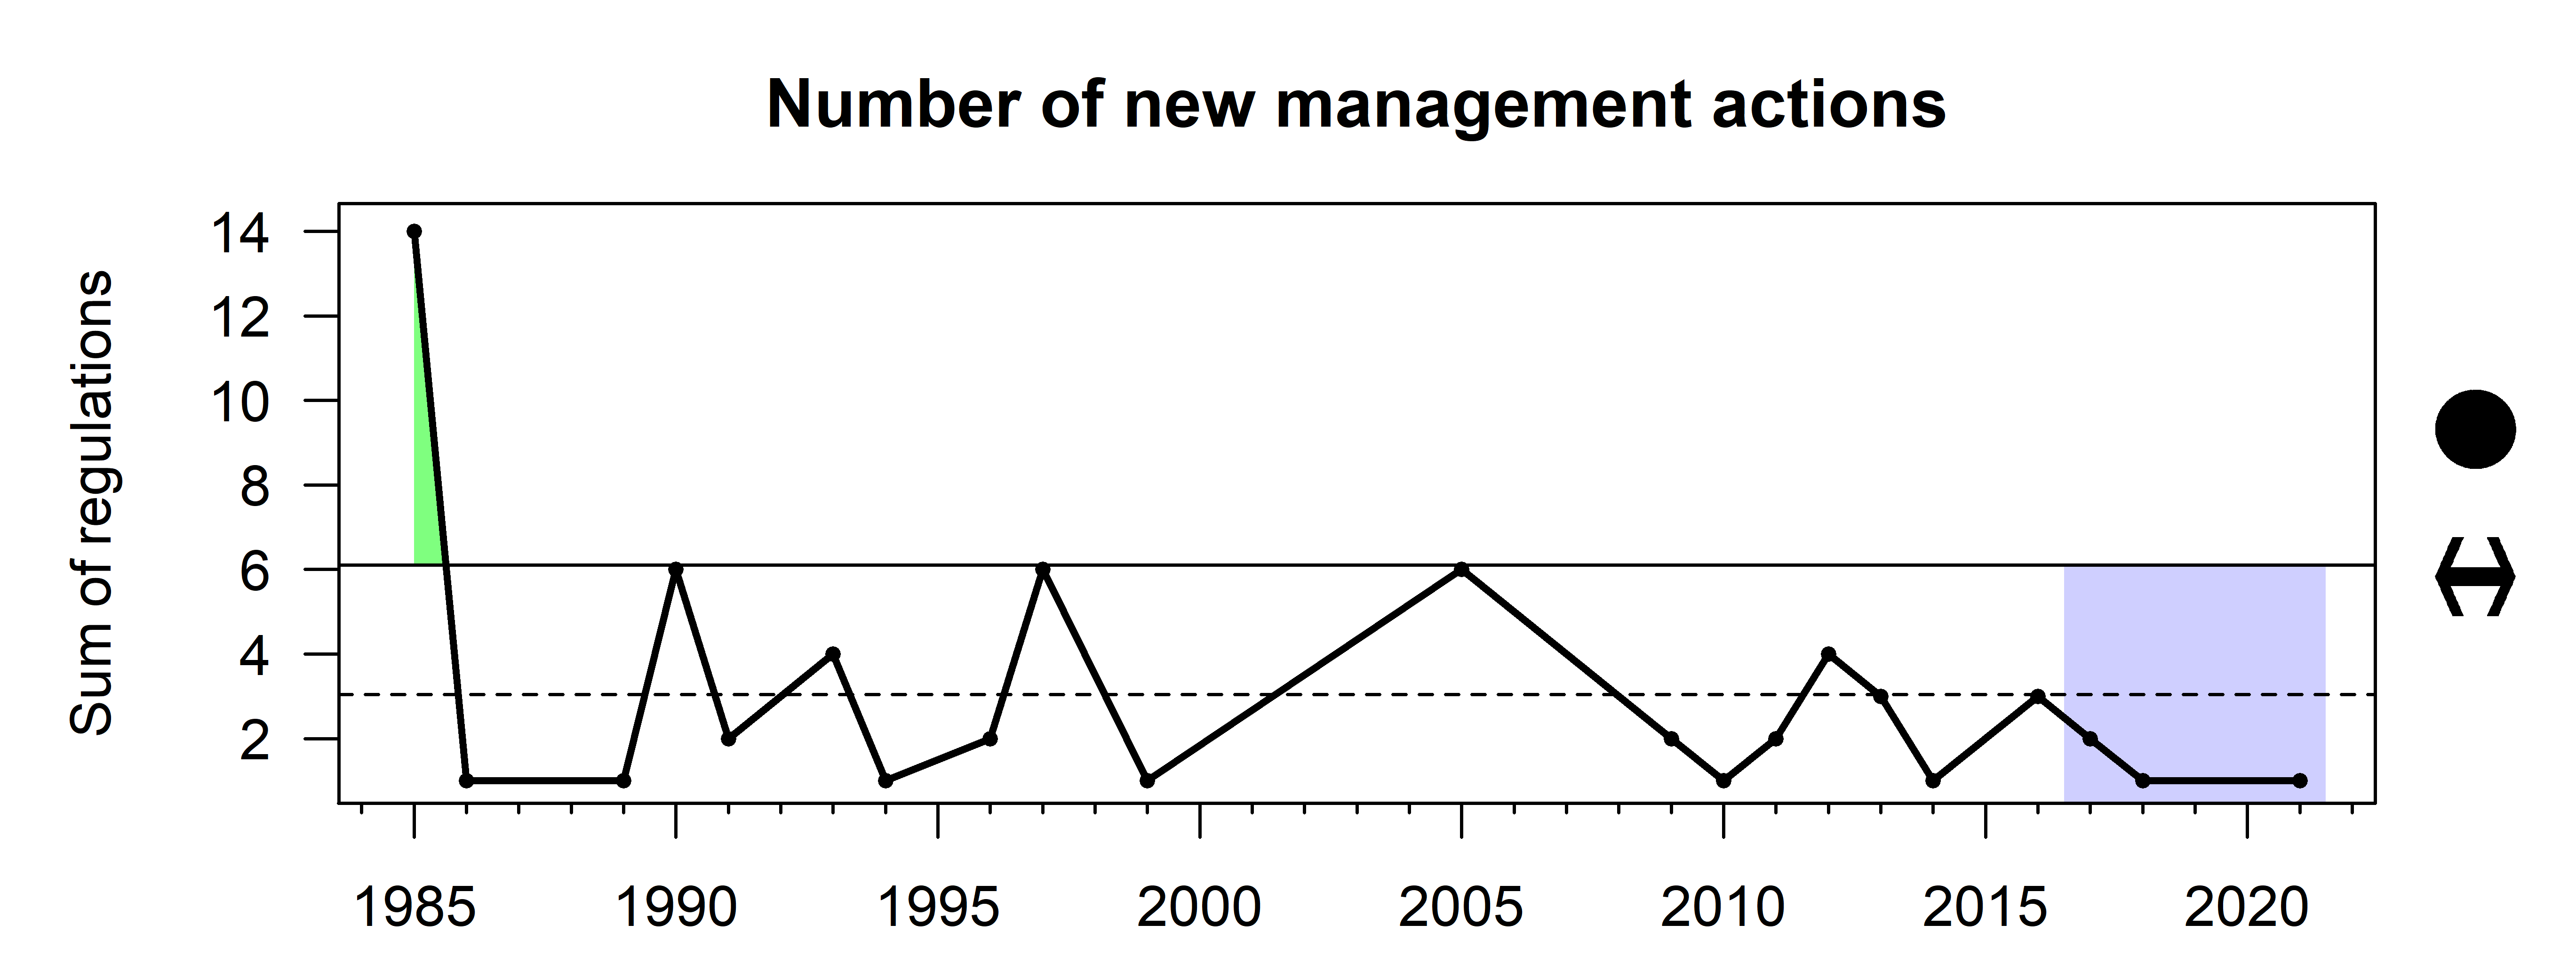
\includegraphics[width=0.75\linewidth,height=\textheight,keepaspectratio]{indicator_plots/FRsection_plot_final.png}

}

\caption{\label{fig-FR}The number of new management actions implemented
in the U.S. Caribbean region based on the annual count of unique Federal
Register sections within all Federal Register notices.}

\end{figure}%

\subsection{Species with informative catch
limits}\label{species-with-informative-catch-limits}

U.S. Caribbean fisheries are highly diverse; over 300 individual species
have been recorded in the landings database and there are 54 stocks or
complexes within the three Island-based Fishery Management Plans. At the
same time, the region is extremely data-limited, with high uncertainty
in landings data and lacking reliable indices of abundance, and most
annual catch limits are derived using Tier 4 of the control rule
included in the FMPs (based on landings over a defined time period). The
percentage of stocks or complexes with annual catch limits informed by
stock assessments is a useful indicator for tracking progress toward
more robust management advice in the region. In recent years, progress
has been made and some stock assessments have been accepted for
management advice (Figure~\ref{fig-tier3}).

\begin{figure}

\centering{

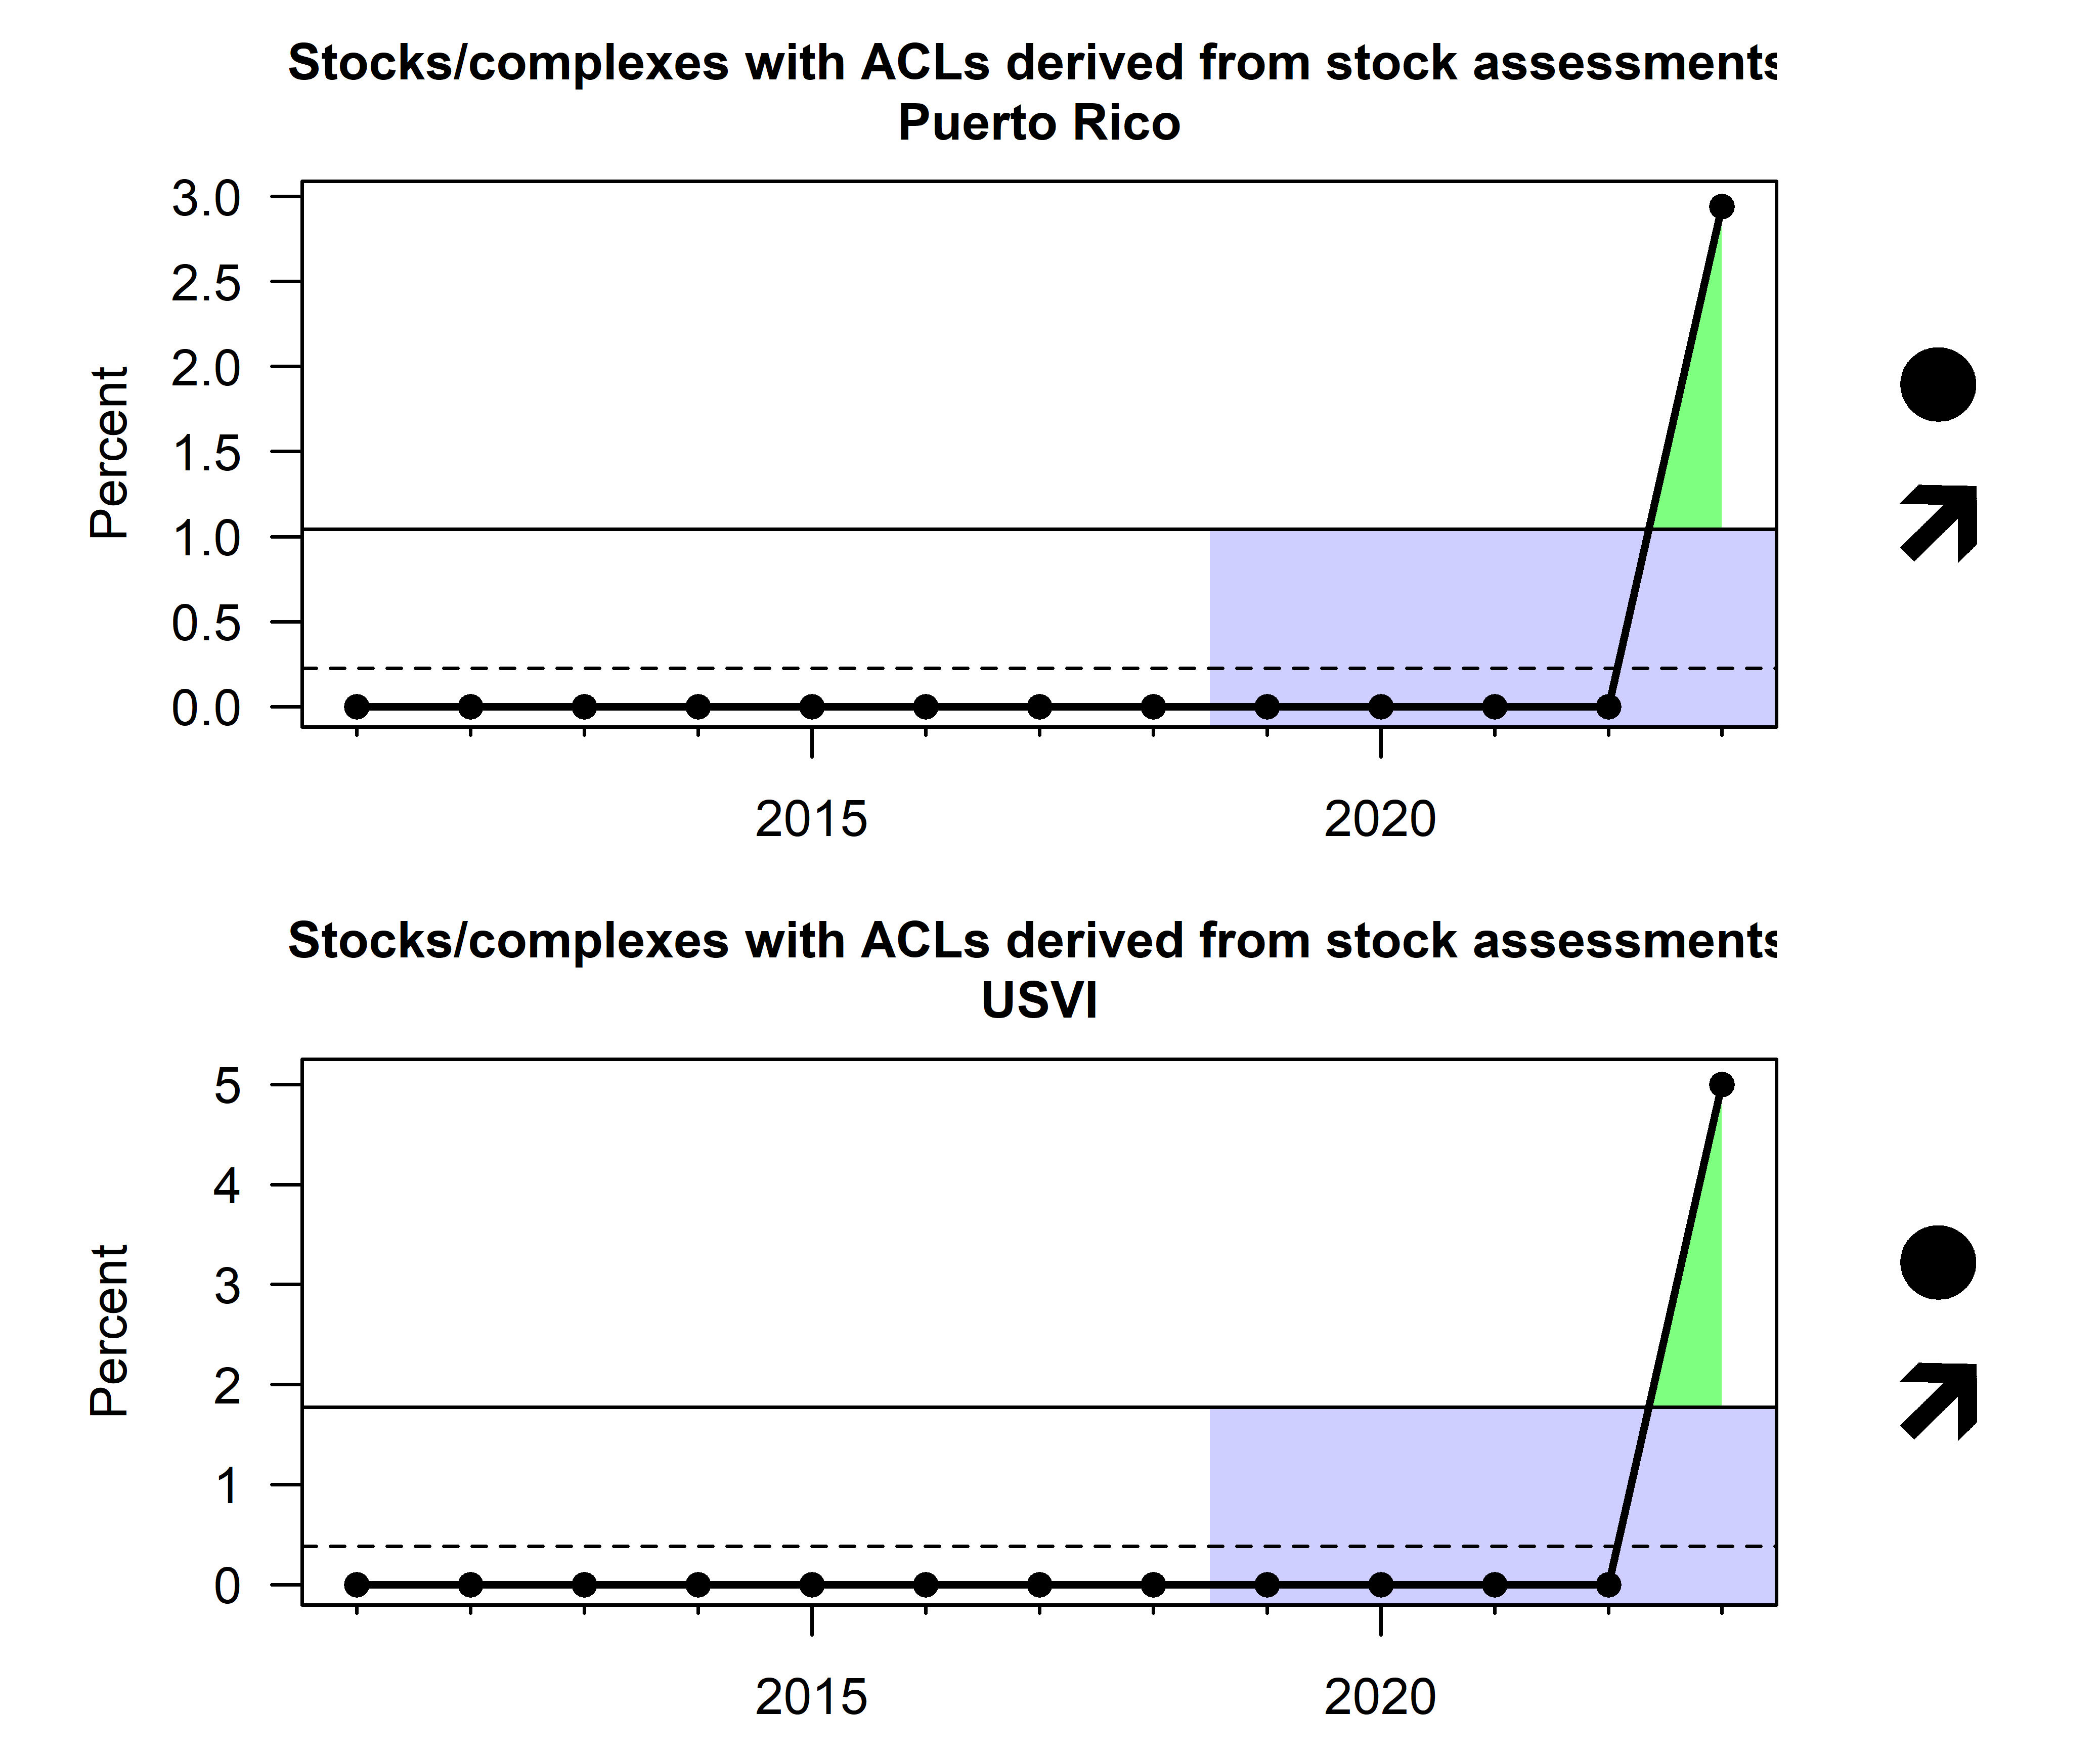
\includegraphics[width=0.75\linewidth,height=\textheight,keepaspectratio]{indicator_plots/tier3_plot_final.png}

}

\caption{\label{fig-tier3}Percent of stocks/complex with informative
annual catch limits as measured by stock assessments in Puerto Rico
(top) and the USVI (bottom).}

\end{figure}%

\subsection{Education and outreach
events}\label{education-and-outreach-events}

Programs such as the Marine Resource Education Program (MREP) and NOAA
SeaGrant have made substantial gains in outreach and education in the
U.S. Caribbean region. MREP is a program developed for fishermen, by
fishermen, and is widely recognized as a key venue for engaging industry
members and building trust. Sea Grant is a federal-academic
collaboration that supports research, education and extension to support
coastal resource conservation, conducting outreach in the form of
workshops and meetings. The number of participants benefiting from MREP
and SeaGrant programs has increased rapidly in recent years. Cumulative
numbers of graduates and attendees are reported because once knowledge
is gained it remains in the fishing community and is also spread by
word-of-mouth (Figure~\ref{fig-outreach}).

\begin{figure}

\centering{

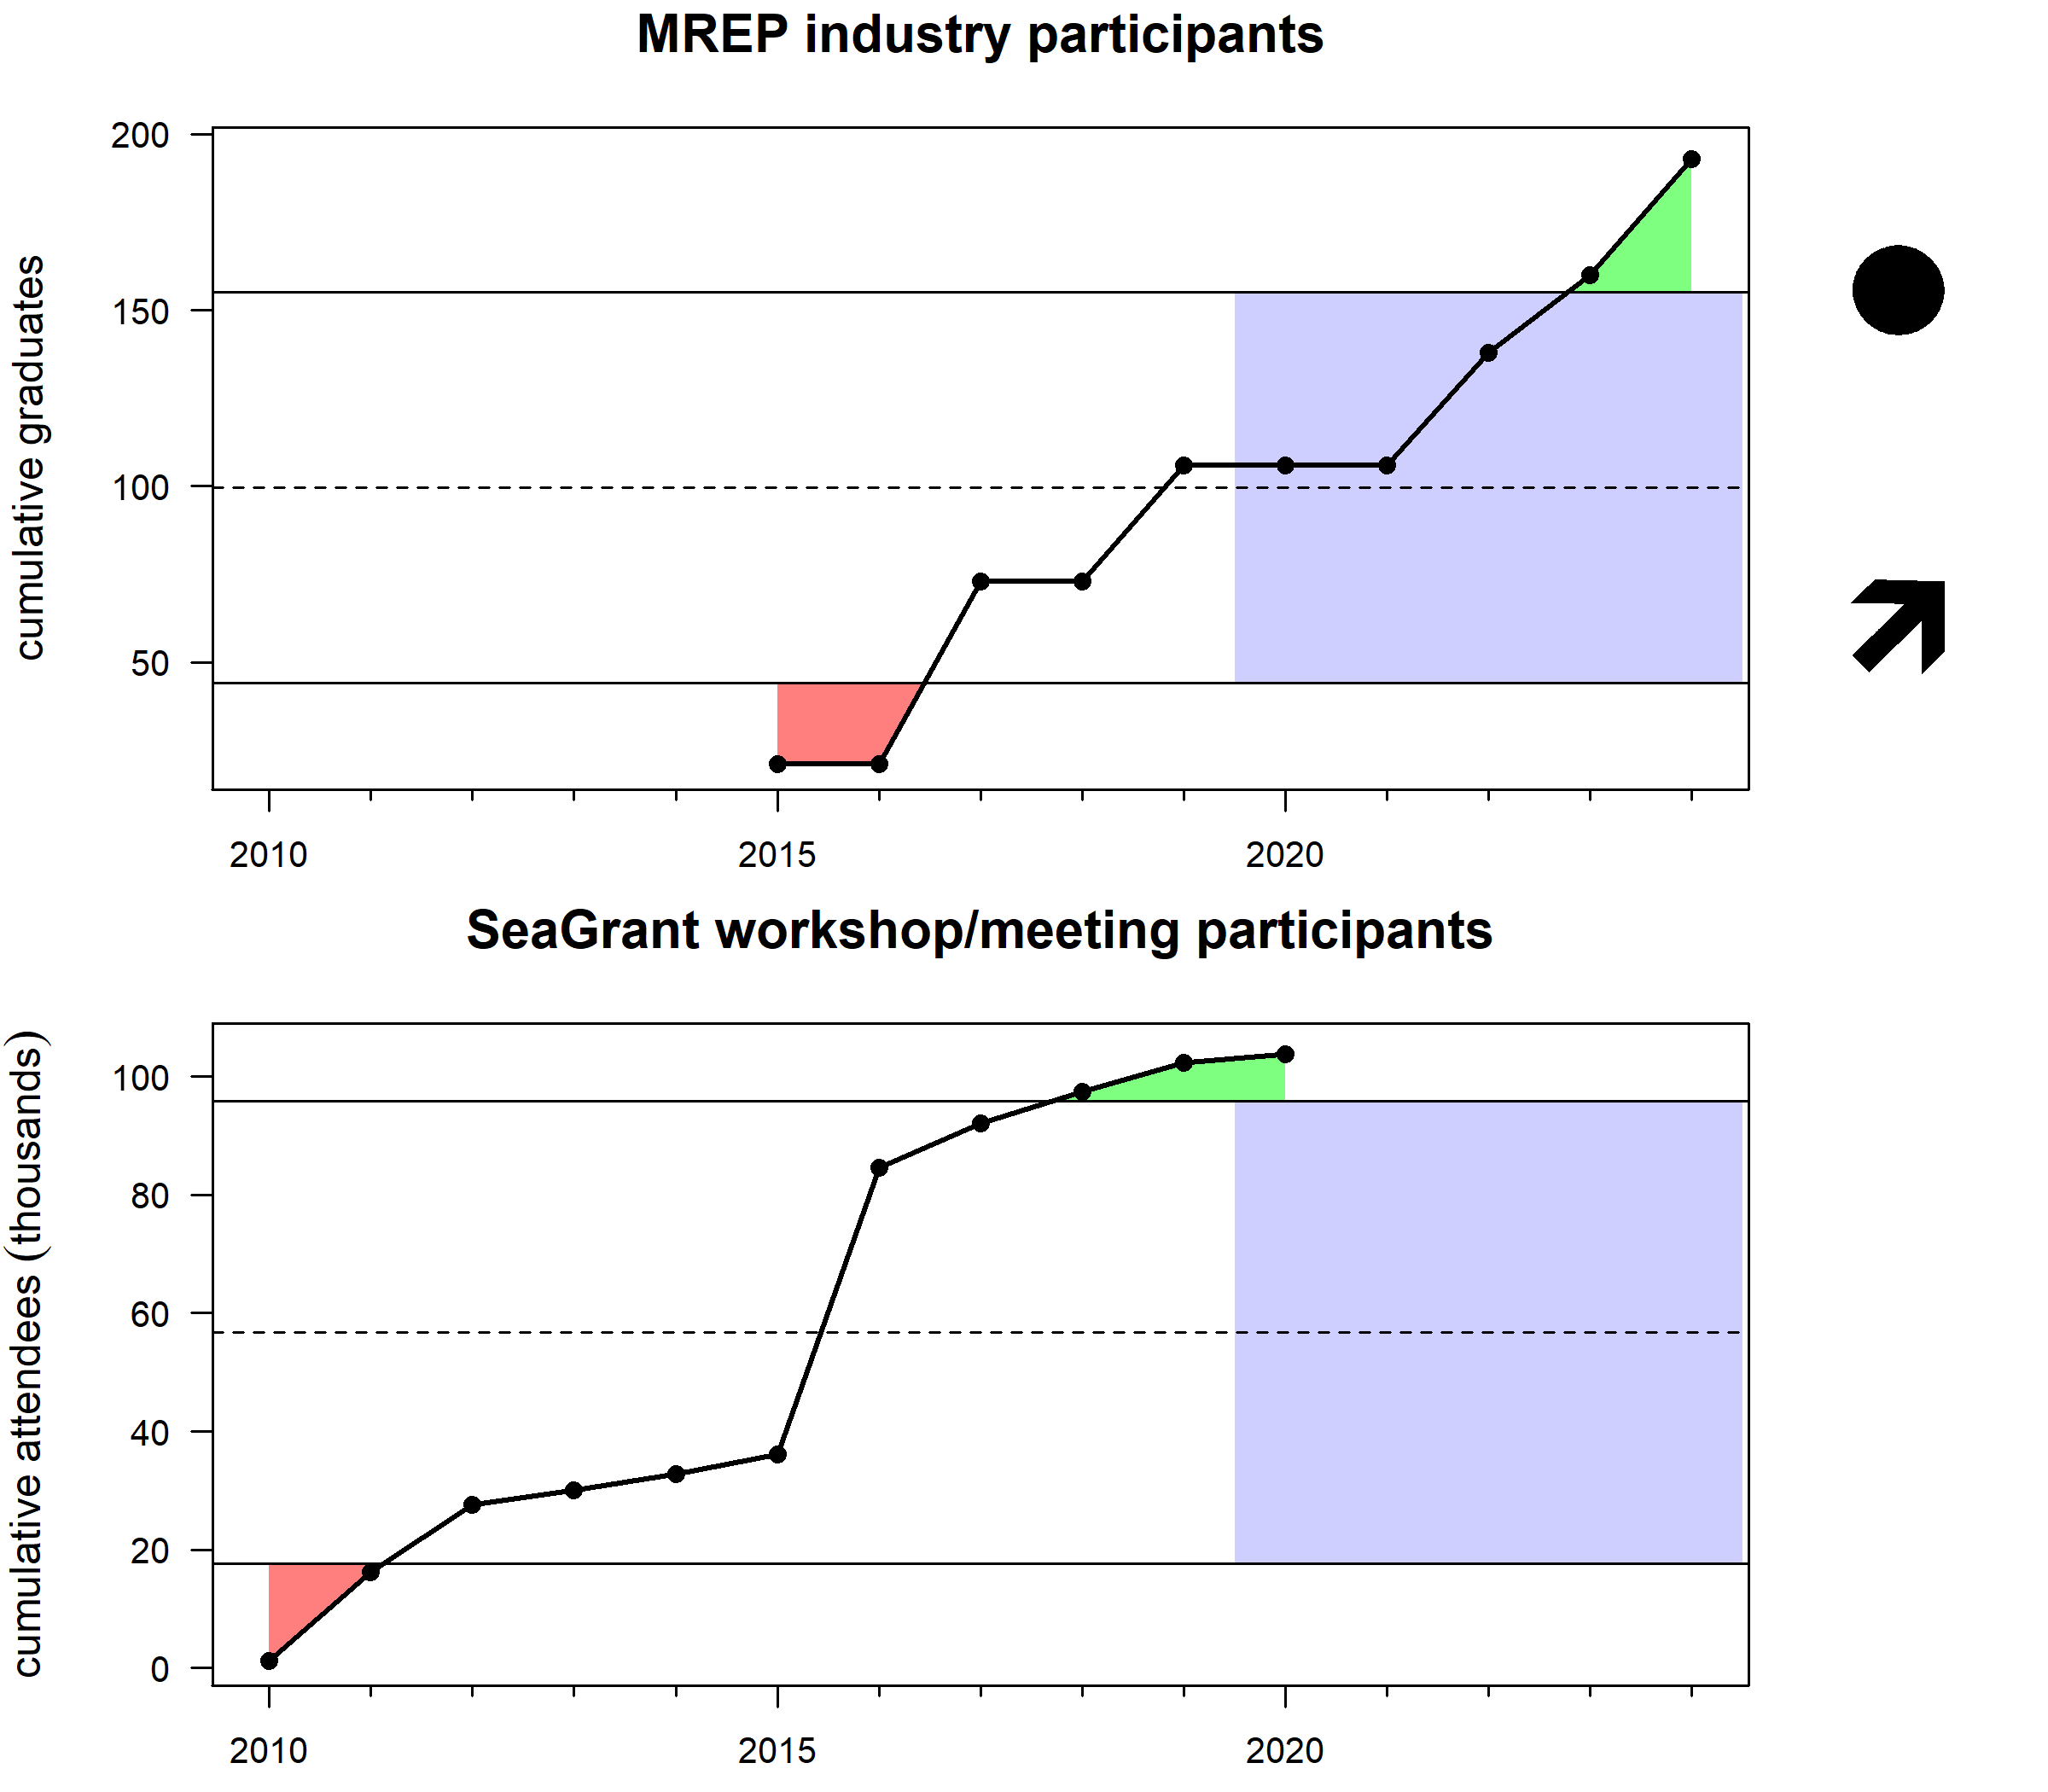
\includegraphics[width=0.75\linewidth,height=\textheight,keepaspectratio]{indicator_plots/outreach_plot_final.png}

}

\caption{\label{fig-outreach}Number of Marine Resource Education Program
industry participants (top) and number of SeaGrant workshop or meeting
participants in the U.S. Caribbean region (bottom).}

\end{figure}%

\subsection{Enforcement actions}\label{enforcement-actions}

The number of recorded law enforcement incidents and patrols may be
indicative of changes in availability of law enforcement resources. The
majority of incidents in the region are created by two NOAA personnel,
in conjunction with multiple state and federal partner agencies. Law
enforcement conducts patrols, investigations, outreach and education,
and compliance assistance to stakeholders. These cumulative efforts aid
in governance of fishery management objectives. Data on federal law
enforcement incidents where the investigating officer was from the
St.~Thomas, USVI or San Juan, PR field offices or the word ``Caribbean''
was mentioned in the brief synopsis were pulled from the NOAA Office of
Law Enforcement NOAA Enforcement Information System (NEIS). Similarly,
data on federal patrols conducted from a field office in PR or USVI were
available in NEIS. Incidents and enforcement have been fairly stable
over the short available time series, with some inter-annual variability
(Figure~\ref{fig-law}).

\begin{figure}

\centering{

\pandocbounded{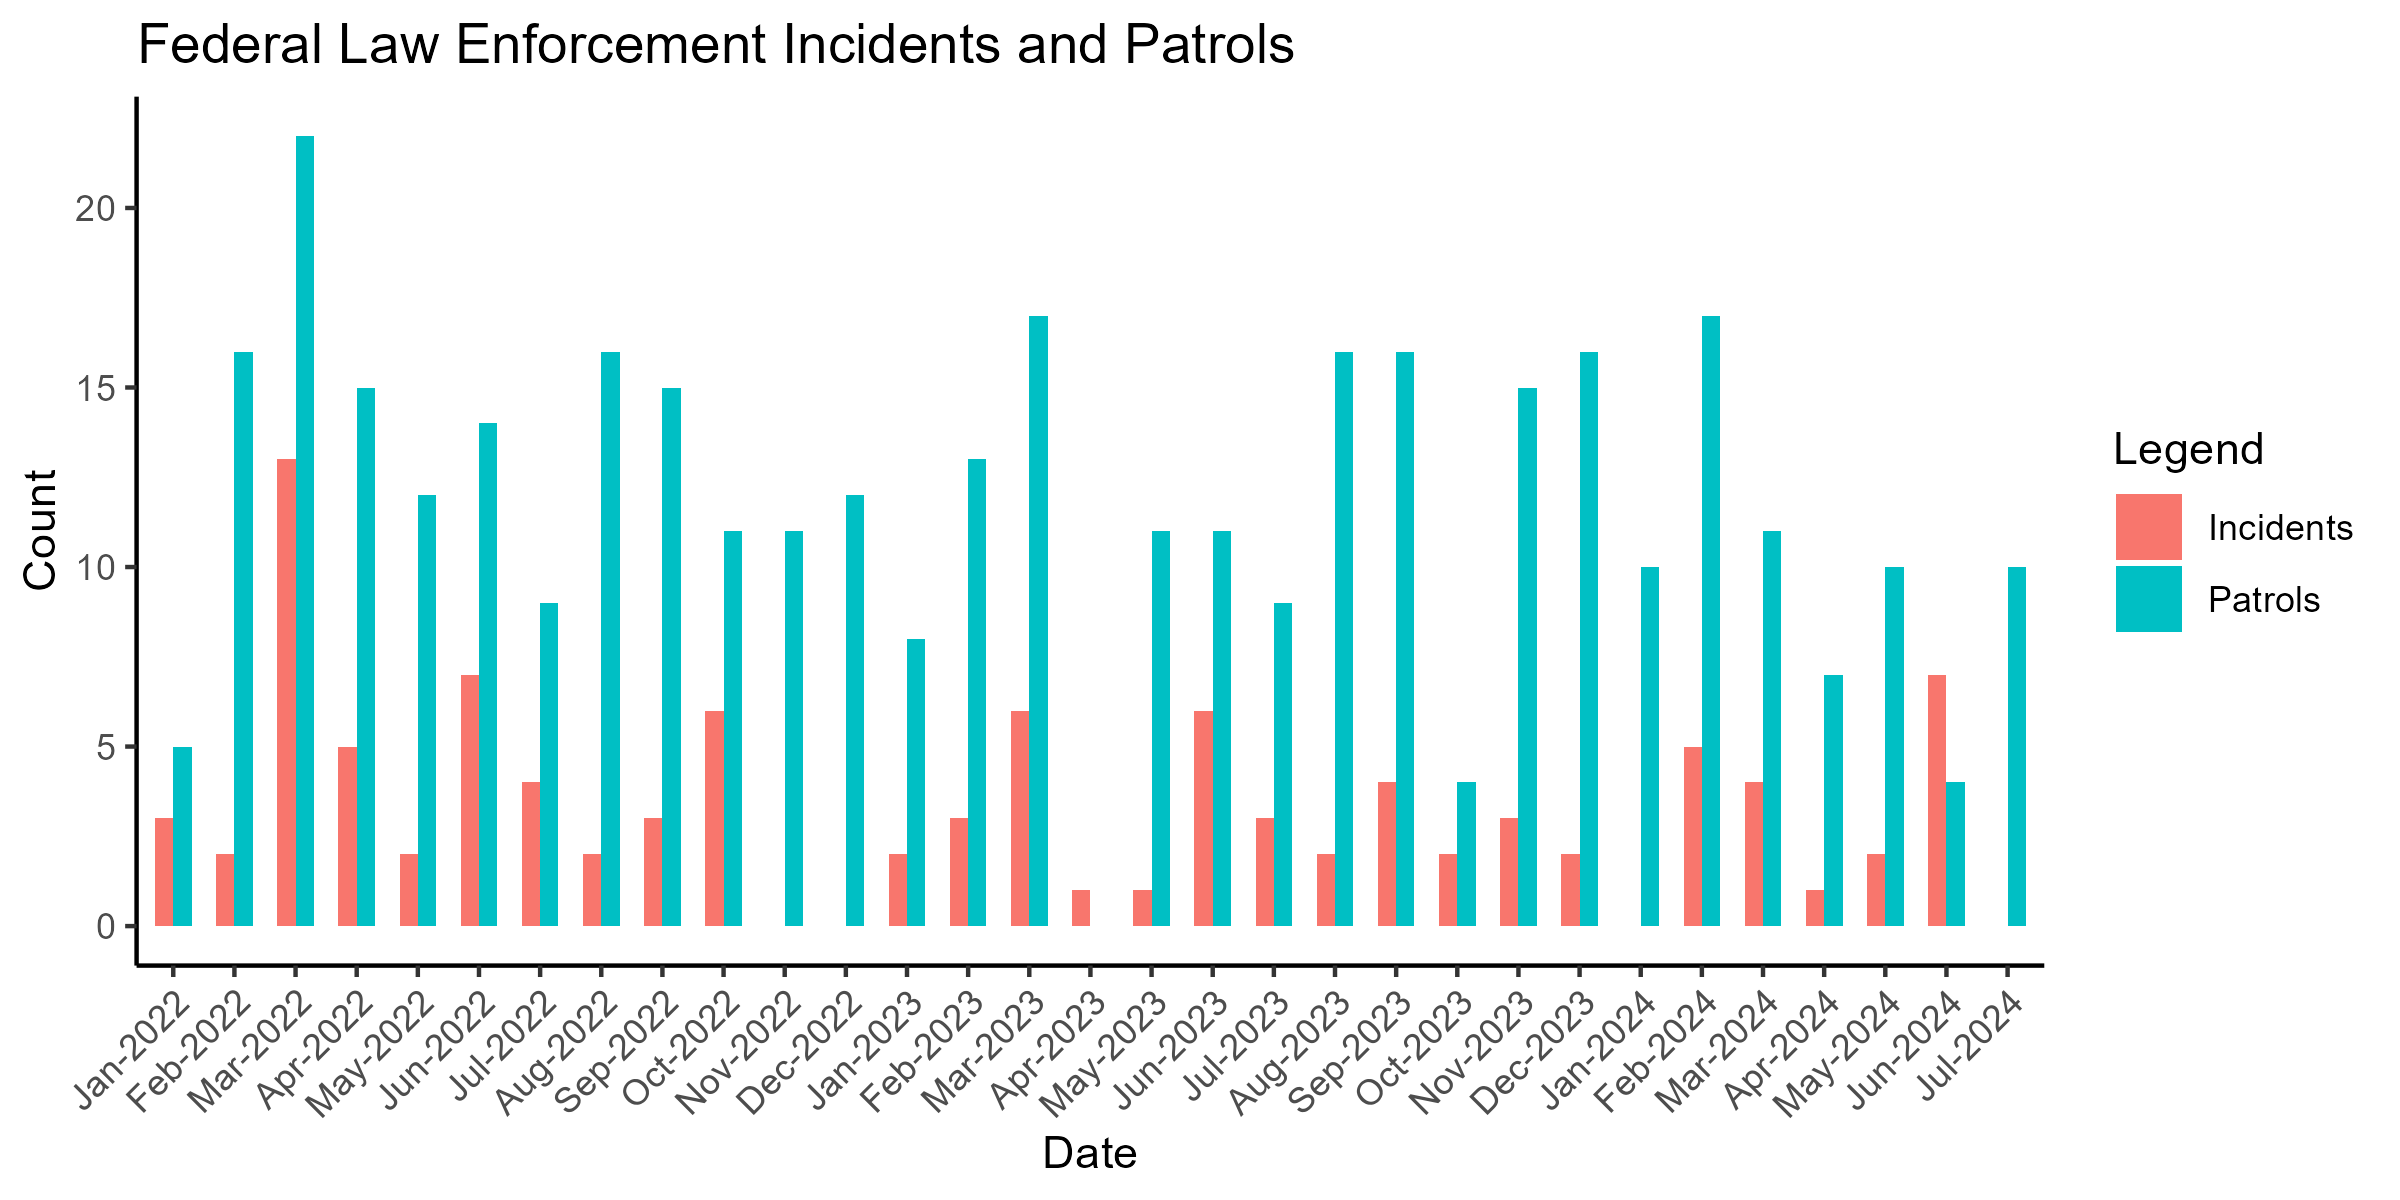
\includegraphics[keepaspectratio]{indicator_plots/enforcement_barplot.png}}

}

\caption{\label{fig-law}Monthly count of federal law enforcement
incidents in the U.S. Caribbean region by date of incident creation
(total n = 101) and monthly count of patrols (including land, sea, and
international trade) conducted from a field office in Puerto Rico or
USVI (total n = 363).}

\end{figure}%

\section{Protection of ecosystems}\label{protection-of-ecosystems}

\subsection{Coral cover and coral species
diversity}\label{coral-cover-and-coral-species-diversity}

Coral reef ecosystem integrity is a major concern for stakeholders in
the U.S. Caribbean region (Seara et al. 2024). The PRCRMP and TRCMP have
measured benthic cover at fixed transects for over two decades, allowing
for a comparison over time. Coral species richness was calculated based
on the average number of hard coral species per 10-m long transect, and
percent coral cover is measured by assigning substrate type to randomly
assigned points within still images of the benthic transects (TCRMP) or
using the continuous intercept method over a fixed transect line
(PRCRMP). Trends in species richness for both Puerto Rico and the USVI
fluctuate over time with no clear trend, although there has been a
sudden decline in recentit years. Percent coral cover has dropped
significantly throughout the 25-year time period with large declines
occurring in 2005 and 2019, coinciding with major bleaching events
(Figure~\ref{fig-coral}).

\begin{figure}

\centering{

\pandocbounded{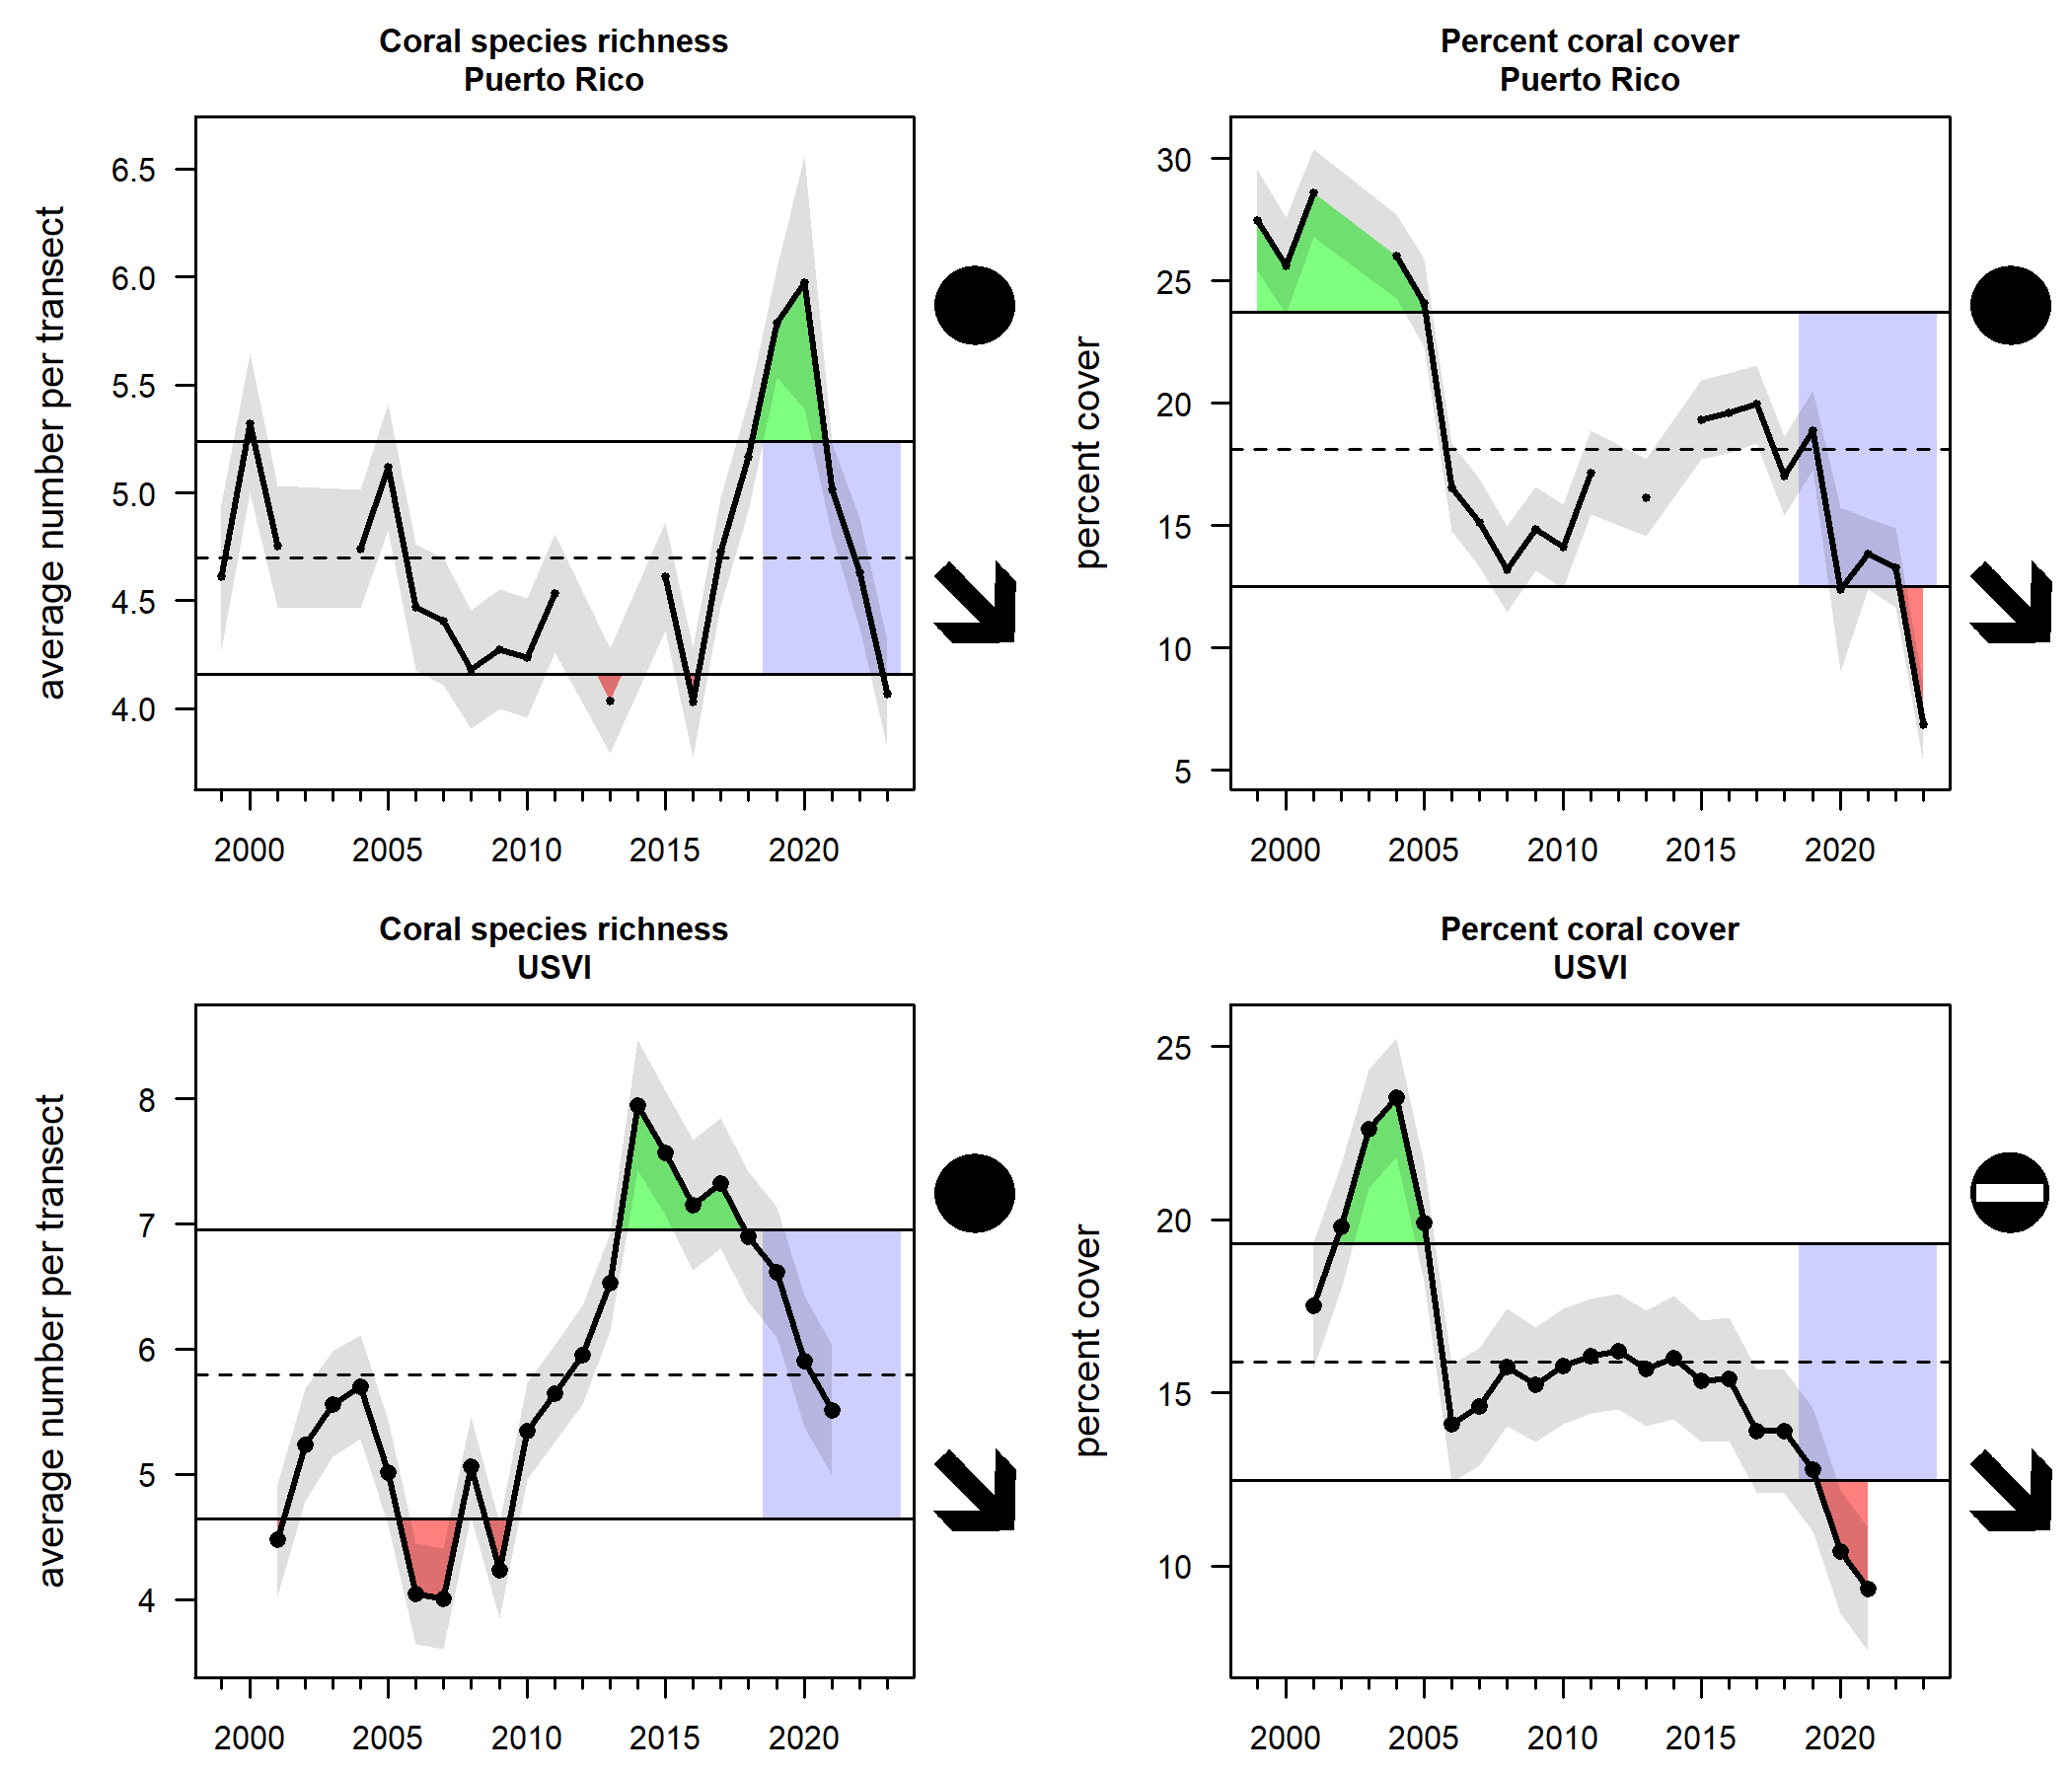
\includegraphics[keepaspectratio]{indicator_plots/coral_spprichness_cover_plot_final.png}}

}

\caption{\label{fig-coral}Percent coral cover and coral species richness
(average number of species per transect) from TCRMP and PRCRMP
biological surveys.}

\end{figure}%

\bookmarksetup{startatroot}

\chapter{Risks to meeting fishery management
objectives}\label{risks-to-meeting-fishery-management-objectives}

In this section, we report indicators that capture identified risks to
the ecosystem that could impact the ability to meet Fishery Management
Plan objectives. Unless otherwise specified, physical indicators
reported for the U.S. Caribbean region were calculated over a bounding
box with limits of longitude 68 degrees W to 64.5 degrees W and latitude
17.5 degrees N to 18.75 degrees N.

\section{Sea surface temperature}\label{sea-surface-temperature}

Ocean temperatures affect species distributions and other aspects of
population dynamics and have impacts on habitats such as coral reefs.
Monthly mean, minimum, and maximum sea surface temperatures were
calculated based on the 1/4 Degree Daily Optimum Interpolation Sea
Surface Temperature (OISST) Analysis (Reynolds et al. 2007). Mean
temperatures in the U.S. Caribbean region have been increasing at an
average rate of 0.25 degrees Celsius per decade. In the last several
years, monthly mean, monthly minimum, and monthly maximum temperatures
have all been well above the historical average, and in the last five
years the temperature trend has been a significant increase
(Figure~\ref{fig-SST}).

\begin{figure}

\centering{

\pandocbounded{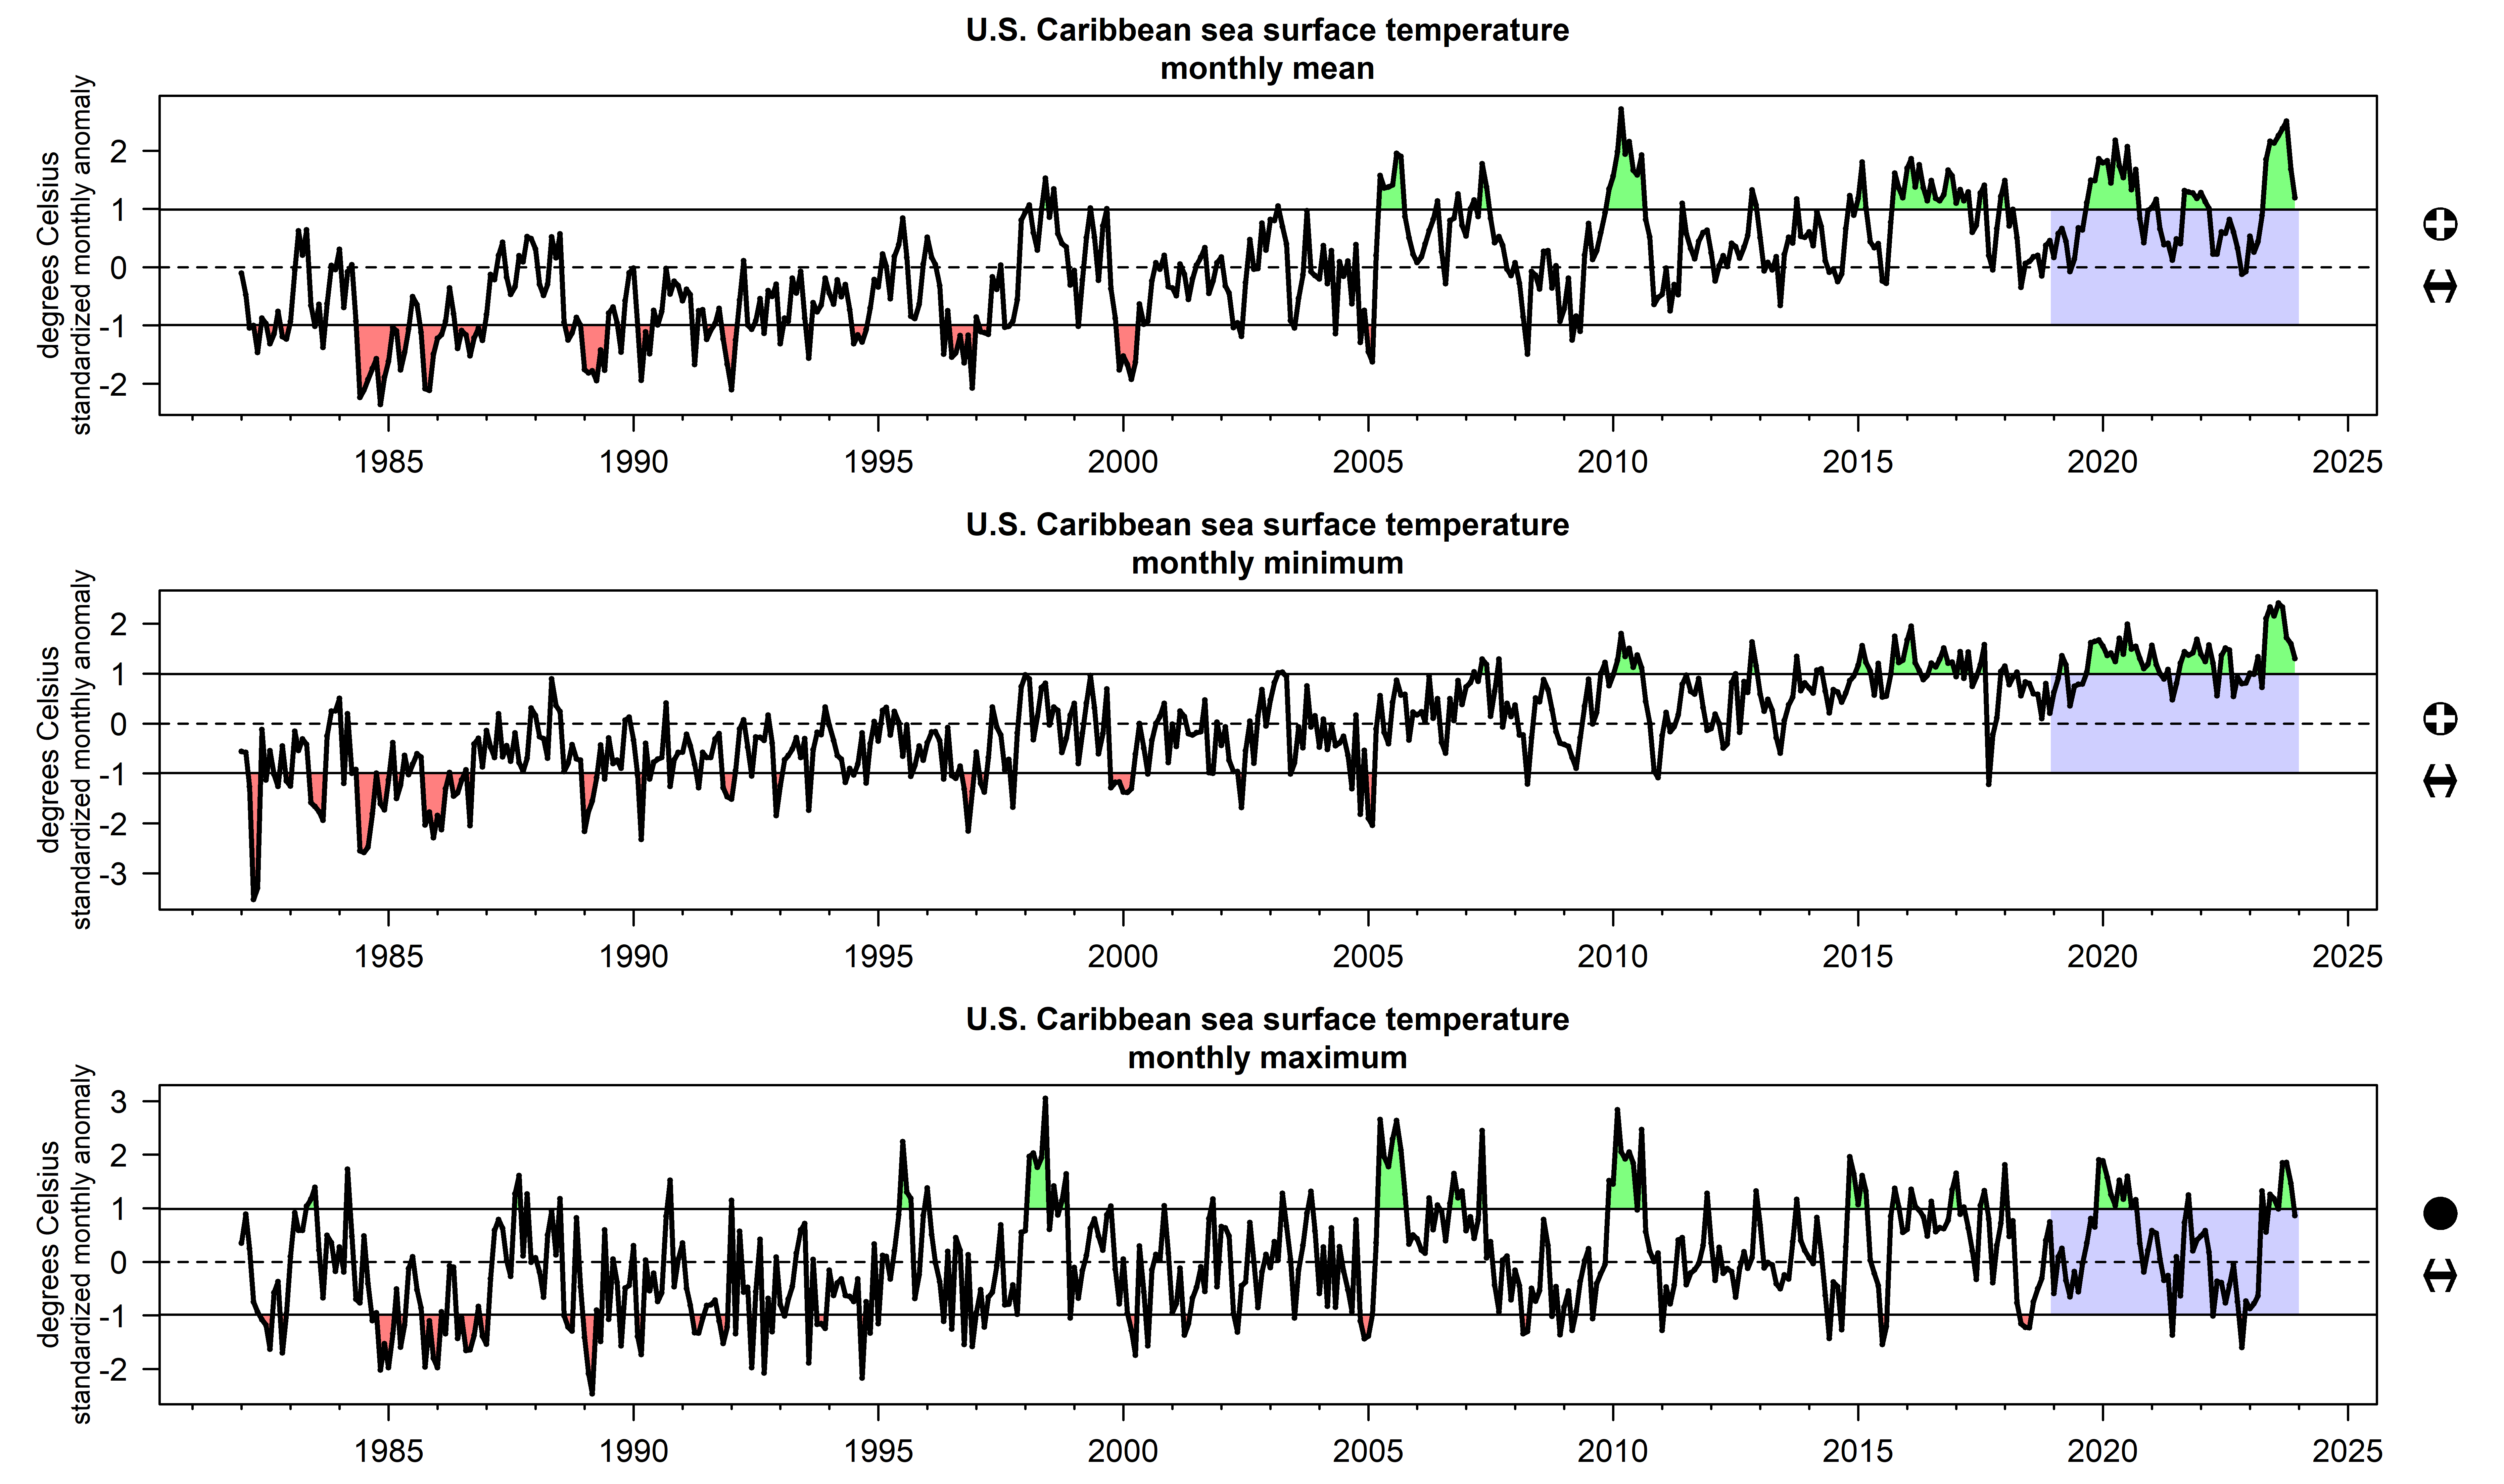
\includegraphics[keepaspectratio]{indicator_plots/Carib_SST_plot_final.png}}

}

\caption{\label{fig-SST}Monthly mean (top), minimum (middle), and
maximum (bottom) sea surface temperature standardized anomalies,
calculated over the U.S. Caribbean region.}

\end{figure}%

\section{Coral bleaching stress}\label{coral-bleaching-stress}

Accumulated heat stress, which can lead to coral bleaching and death, is
measured by summing degree heating weeks for the previous 12-week period
from sea surface temperature data (NOAA Coral Reef Watch 2019).
Bleaching stress was generally below average prior to the mid-2000s,
when a sudden bleaching event occurred in 2005; this event is now the
second most severe event in the time series. In 2024, a bleaching event
of unprecedented severity occurred across the U.S. Caribbean and beyond
(Figure~\ref{fig-DHW}).

\begin{figure}

\centering{

\pandocbounded{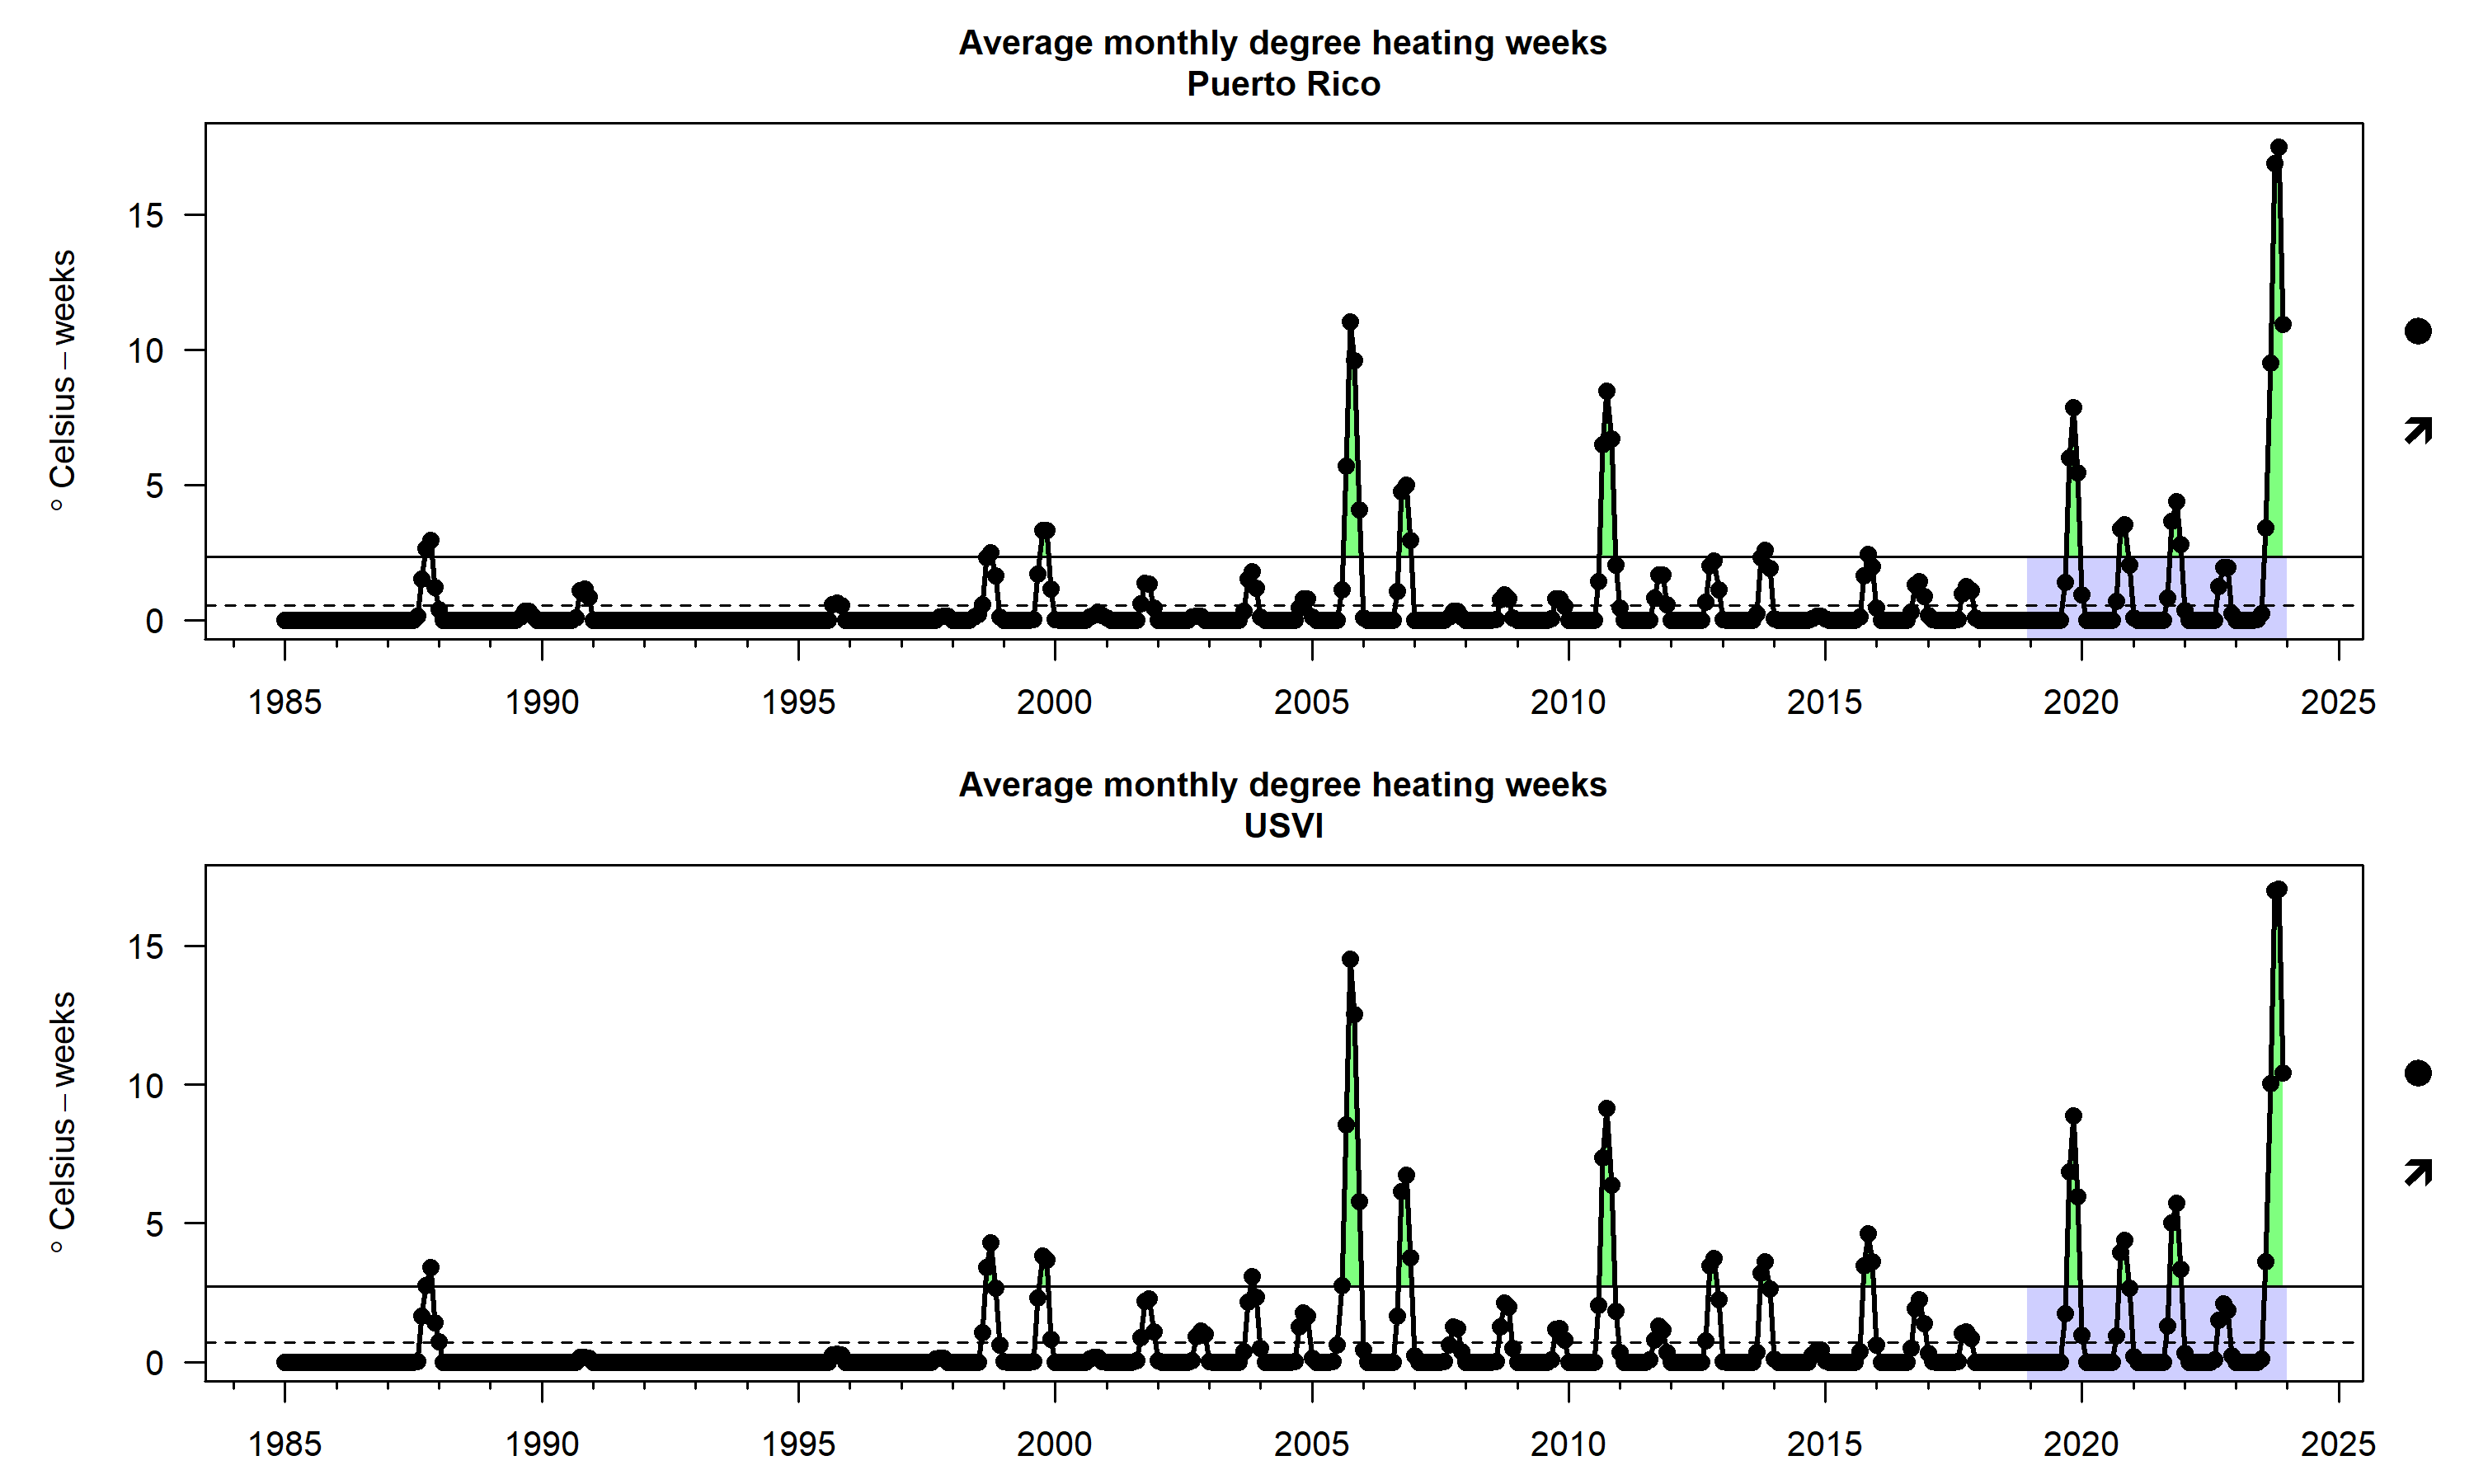
\includegraphics[keepaspectratio]{indicator_plots/DegreeHeatingWeeks_plot_final.png}}

}

\caption{\label{fig-DHW}Average monthly degree heating week values as
reported by NOAA Coral Reef Watch Virtual Stations for Puerto Rico (top)
and USVI (bottom).}

\end{figure}%

\section{Ocean acidification}\label{ocean-acidification}

Ocean and coastal acidification can impact organisms directly or
indirectly; a decrease in aragonite saturation state can make it
difficult for corals and other calcifying organisms to form hard
structures, contributing to lower reproduction or survival rates. When
the aragonite saturation state falls below 3, corals begin to experience
physiological stress, and calcification rates decline and skeletal
structure begins to weaken; calcification stops completely and skeletal
structure begins to dissolve at aragonite saturation states below 1
(Andersson et al. 2009). In-situ measurements of aragonite saturation
states are scarce, and a synoptic long-term view is only available from
modeled products. Aragonite saturation state was derived for the U.S.
Caribbean region from the MOM-TOPAZ hindcast (Gomez and Lee 2023). An
overall negative trend occurs, with an acceleration of this trend
apparent after 2008 (Figure~\ref{fig-OA}).

\begin{figure}

\centering{

\pandocbounded{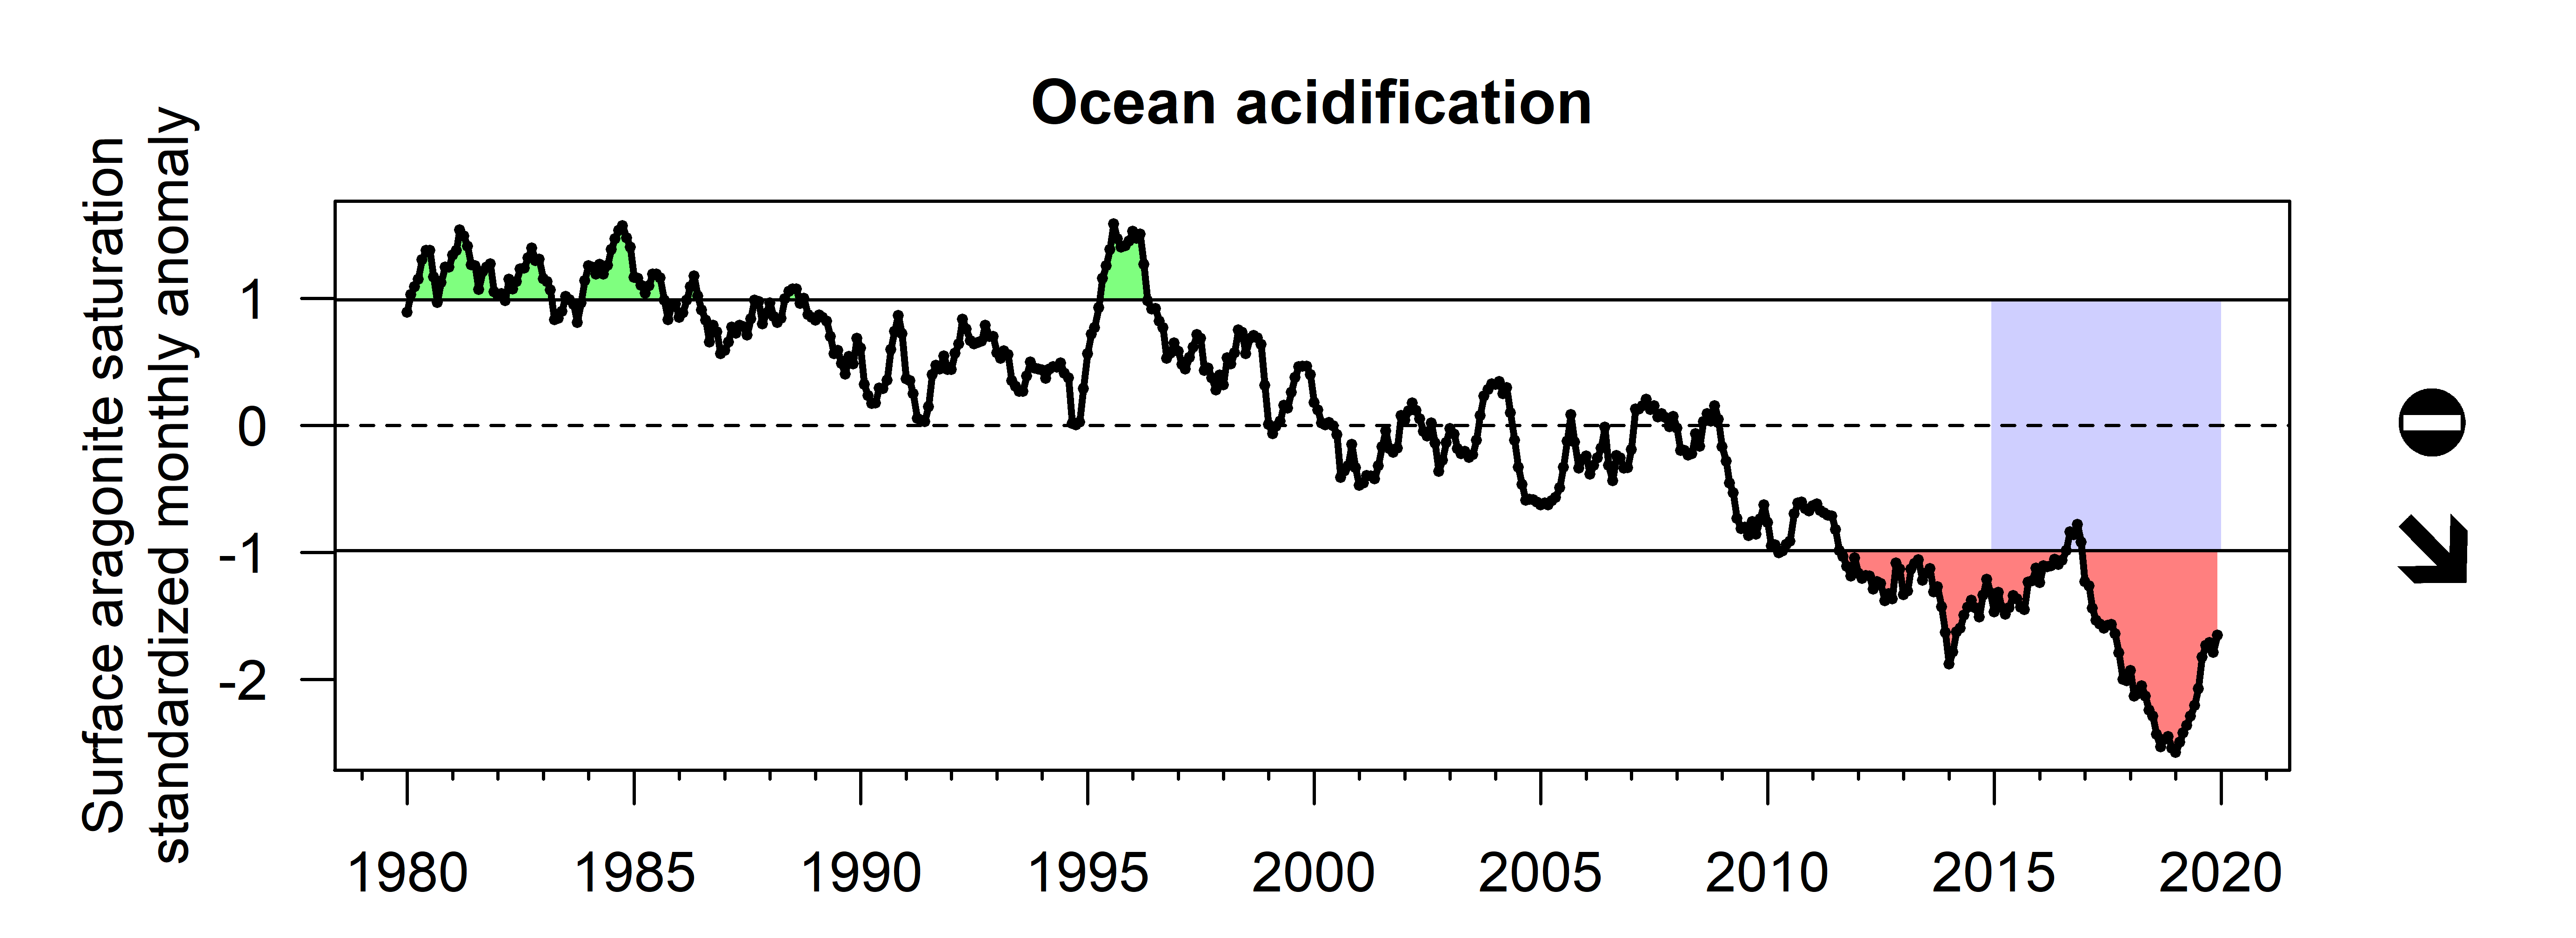
\includegraphics[keepaspectratio]{indicator_plots/OA_plot_final.png}}

}

\caption{\label{fig-OA}Ocean acidification as measured by modeled
surface aragonite saturation state, shown as standardized monthly
anomalies for the U.S. Caribbean region.}

\end{figure}%

\section{Hurricane activity}\label{hurricane-activity}

Hurricane activity can be captured by the accumulated cyclone energy
(ACE) index, a measure of overall tropical cyclone activity measured as
the sum of squared wind speeds. The ACE index was calculated for storms
that track within the U.S. Caribbean region as documented by the
International Best Track Archive for Climate Stewardship database (Knapp
et al. 2010). The index has fluctuated throughout the past seven
decades, with multiple notable peaks (Figure~\ref{fig-ACE}). During the
year 2017, hurricane activity was at an unprecedented high, due to two
major hurricanes that struck the islands: Irma and Maria.

\begin{figure}

\centering{


\includegraphics[width=0.75\linewidth,height=\textheight,keepaspectratio]{indicator_plots/ACEindex_plot_final.png}

}

\caption{\label{fig-ACE}Annual accumulated cyclone energy index,
calculated as the sum of squared 6-hourly reported wind speeds for
storms tracking through the U.S. Caribbean region.}

\end{figure}%

\section{Earthquake activity}\label{earthquake-activity}

Earthquakes can induce landslides and cause impacts to infrastructure
including homes and the electrical grid, and can be a source of stress
in the affected human population (Agar et al. 2022). Individual seismic
events are reported by the United States Geological Survey (USGS) in
near real-time (Sumy, Welti, and Hubenthal 2020). A major earthquake
swarm occurred in Southwest Puerto Rico in early 2020; in this year
there were over 400 events of greater than 3.5 magnitude on the Richter
scale (Figure~\ref{fig-quakes}).

\begin{figure}

\centering{

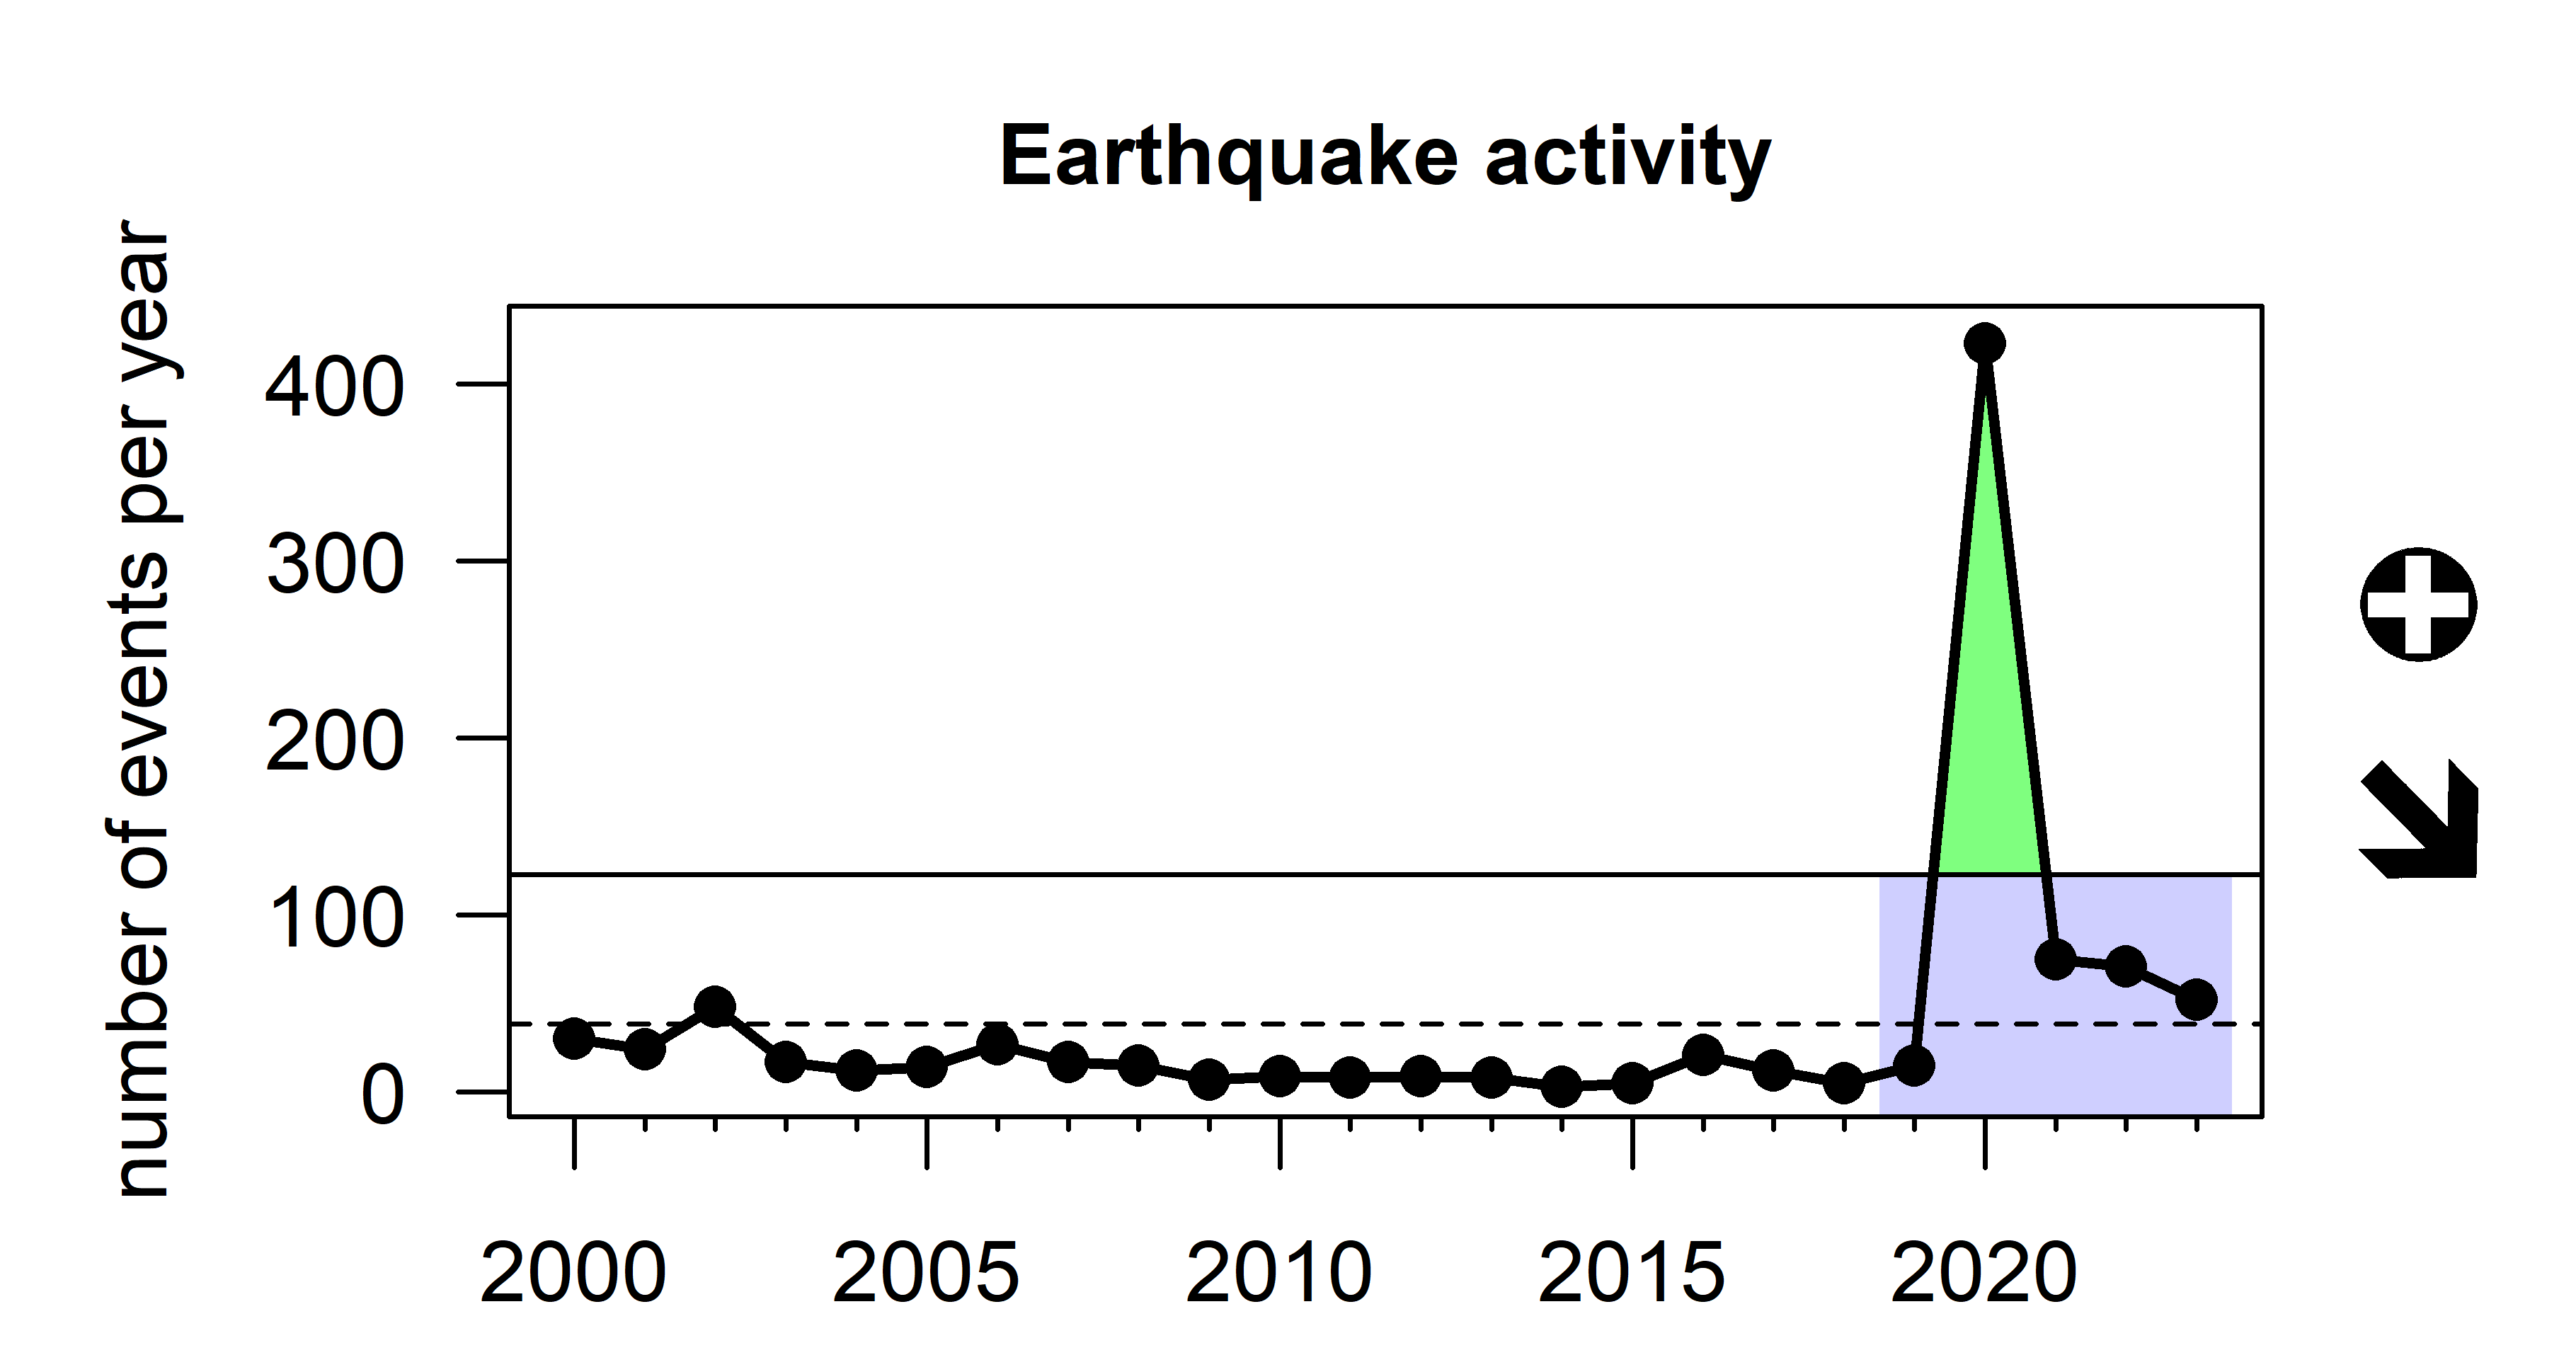
\includegraphics[width=0.75\linewidth,height=\textheight,keepaspectratio]{indicator_plots/earthquakes_plot_final.png}

}

\caption{\label{fig-quakes}Number of seismic events of \textgreater3.5
magnitude occurring annually in the U.S. Caribbean.}

\end{figure}%

\section{Point source pollution}\label{point-source-pollution}

Impacts from terrestrial pollution can be captured from several
databases maintained by the Environmental Protection Agency (EPA). These
databases provide information on companies that have been issued permits
to discharge wastewater into rivers, on the release of toxic chemicals
and waste management activities at facilities, and on sites declared
through the Comprehensive Environmental Response, Compensation, and
Liability Act (commonly known as Superfund sites). The number of
pollution sites reported increased in the 2000s, but has decreased
slightly in both Puerto Rico and USVI in recent years
(Figure~\ref{fig-pollution}). Note that this indicator does not
represent the timing of when pollution was impacting the ecosystem, but
rather the timing of investigation and registration in EPA's monitoring
program or attention to the environmental impacts of pollution.

\begin{figure}

\centering{

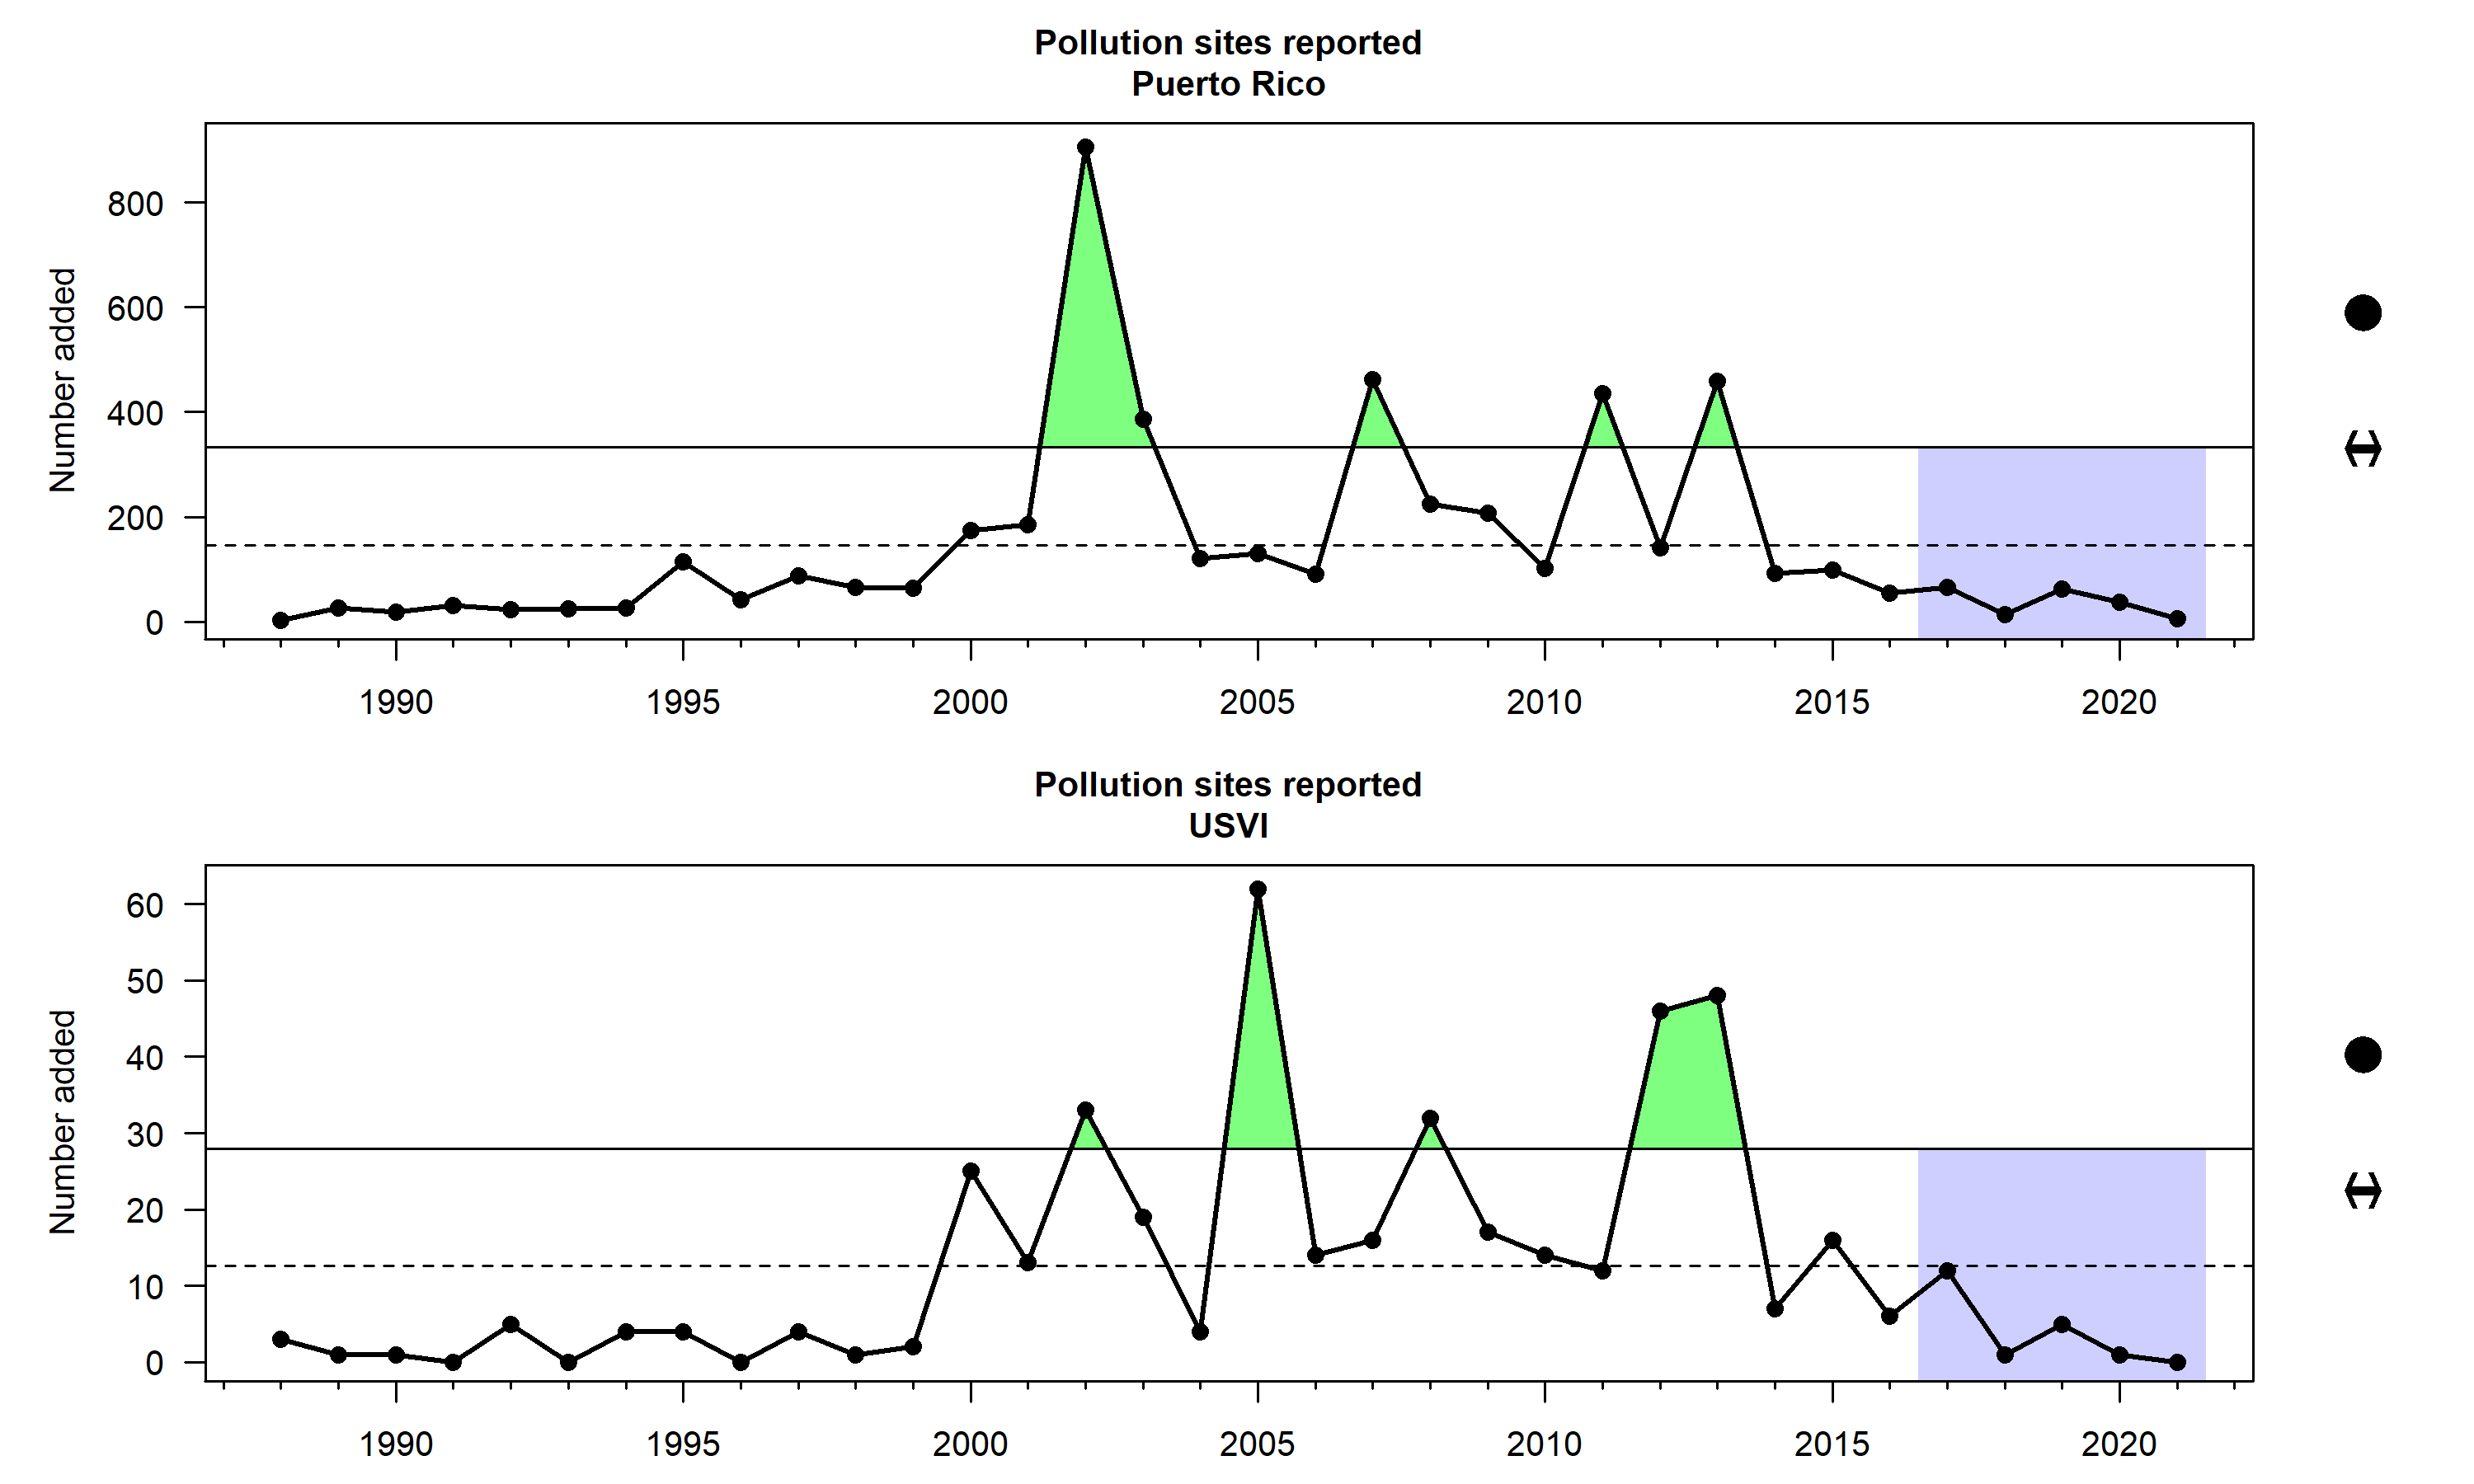
\includegraphics[width=0.75\linewidth,height=\textheight,keepaspectratio]{indicator_plots/pollution_plot_final.png}

}

\caption{\label{fig-pollution}Annual count of identified point source
polluters in the U.S. Caribbean based on TRI sites (Toxic Release
Inventory), Superfund sites (Superfund Enterprise Management System),
National Compliance Database listed sites, and Brownfield sites
identified in Puerto Rico (top) and the USVI (bottom).}

\end{figure}%

\section{Turbidity}\label{turbidity}

Coastal pollution, runoff, and water quality issues are of major concern
to fishing-dependent communities in the U.S. Caribbean (Seara et al.
2024). Water clarity can be measured by the diffuse attenuation
coefficient, which indicates how strongly light intensity is attenuated
within the water column; however, satellite sensors cannot differentiate
between organic and inorganic water particles contributing to water
clarity. NOAA's Coastwatch program provides estimates of the attenuation
coefficient for penetration of light at 490nm (Wang, Son, and Harding
Jr. 2009) based on multiple satellite sensors. No overall trend is
apparent in any of the U.S. Caribbean islands, although there is
increasing variability in turbidity values over time. Elevated anomalies
in Puerto Rico in the year 2017 are likely due to hurricane activity.

\begin{figure}

\centering{

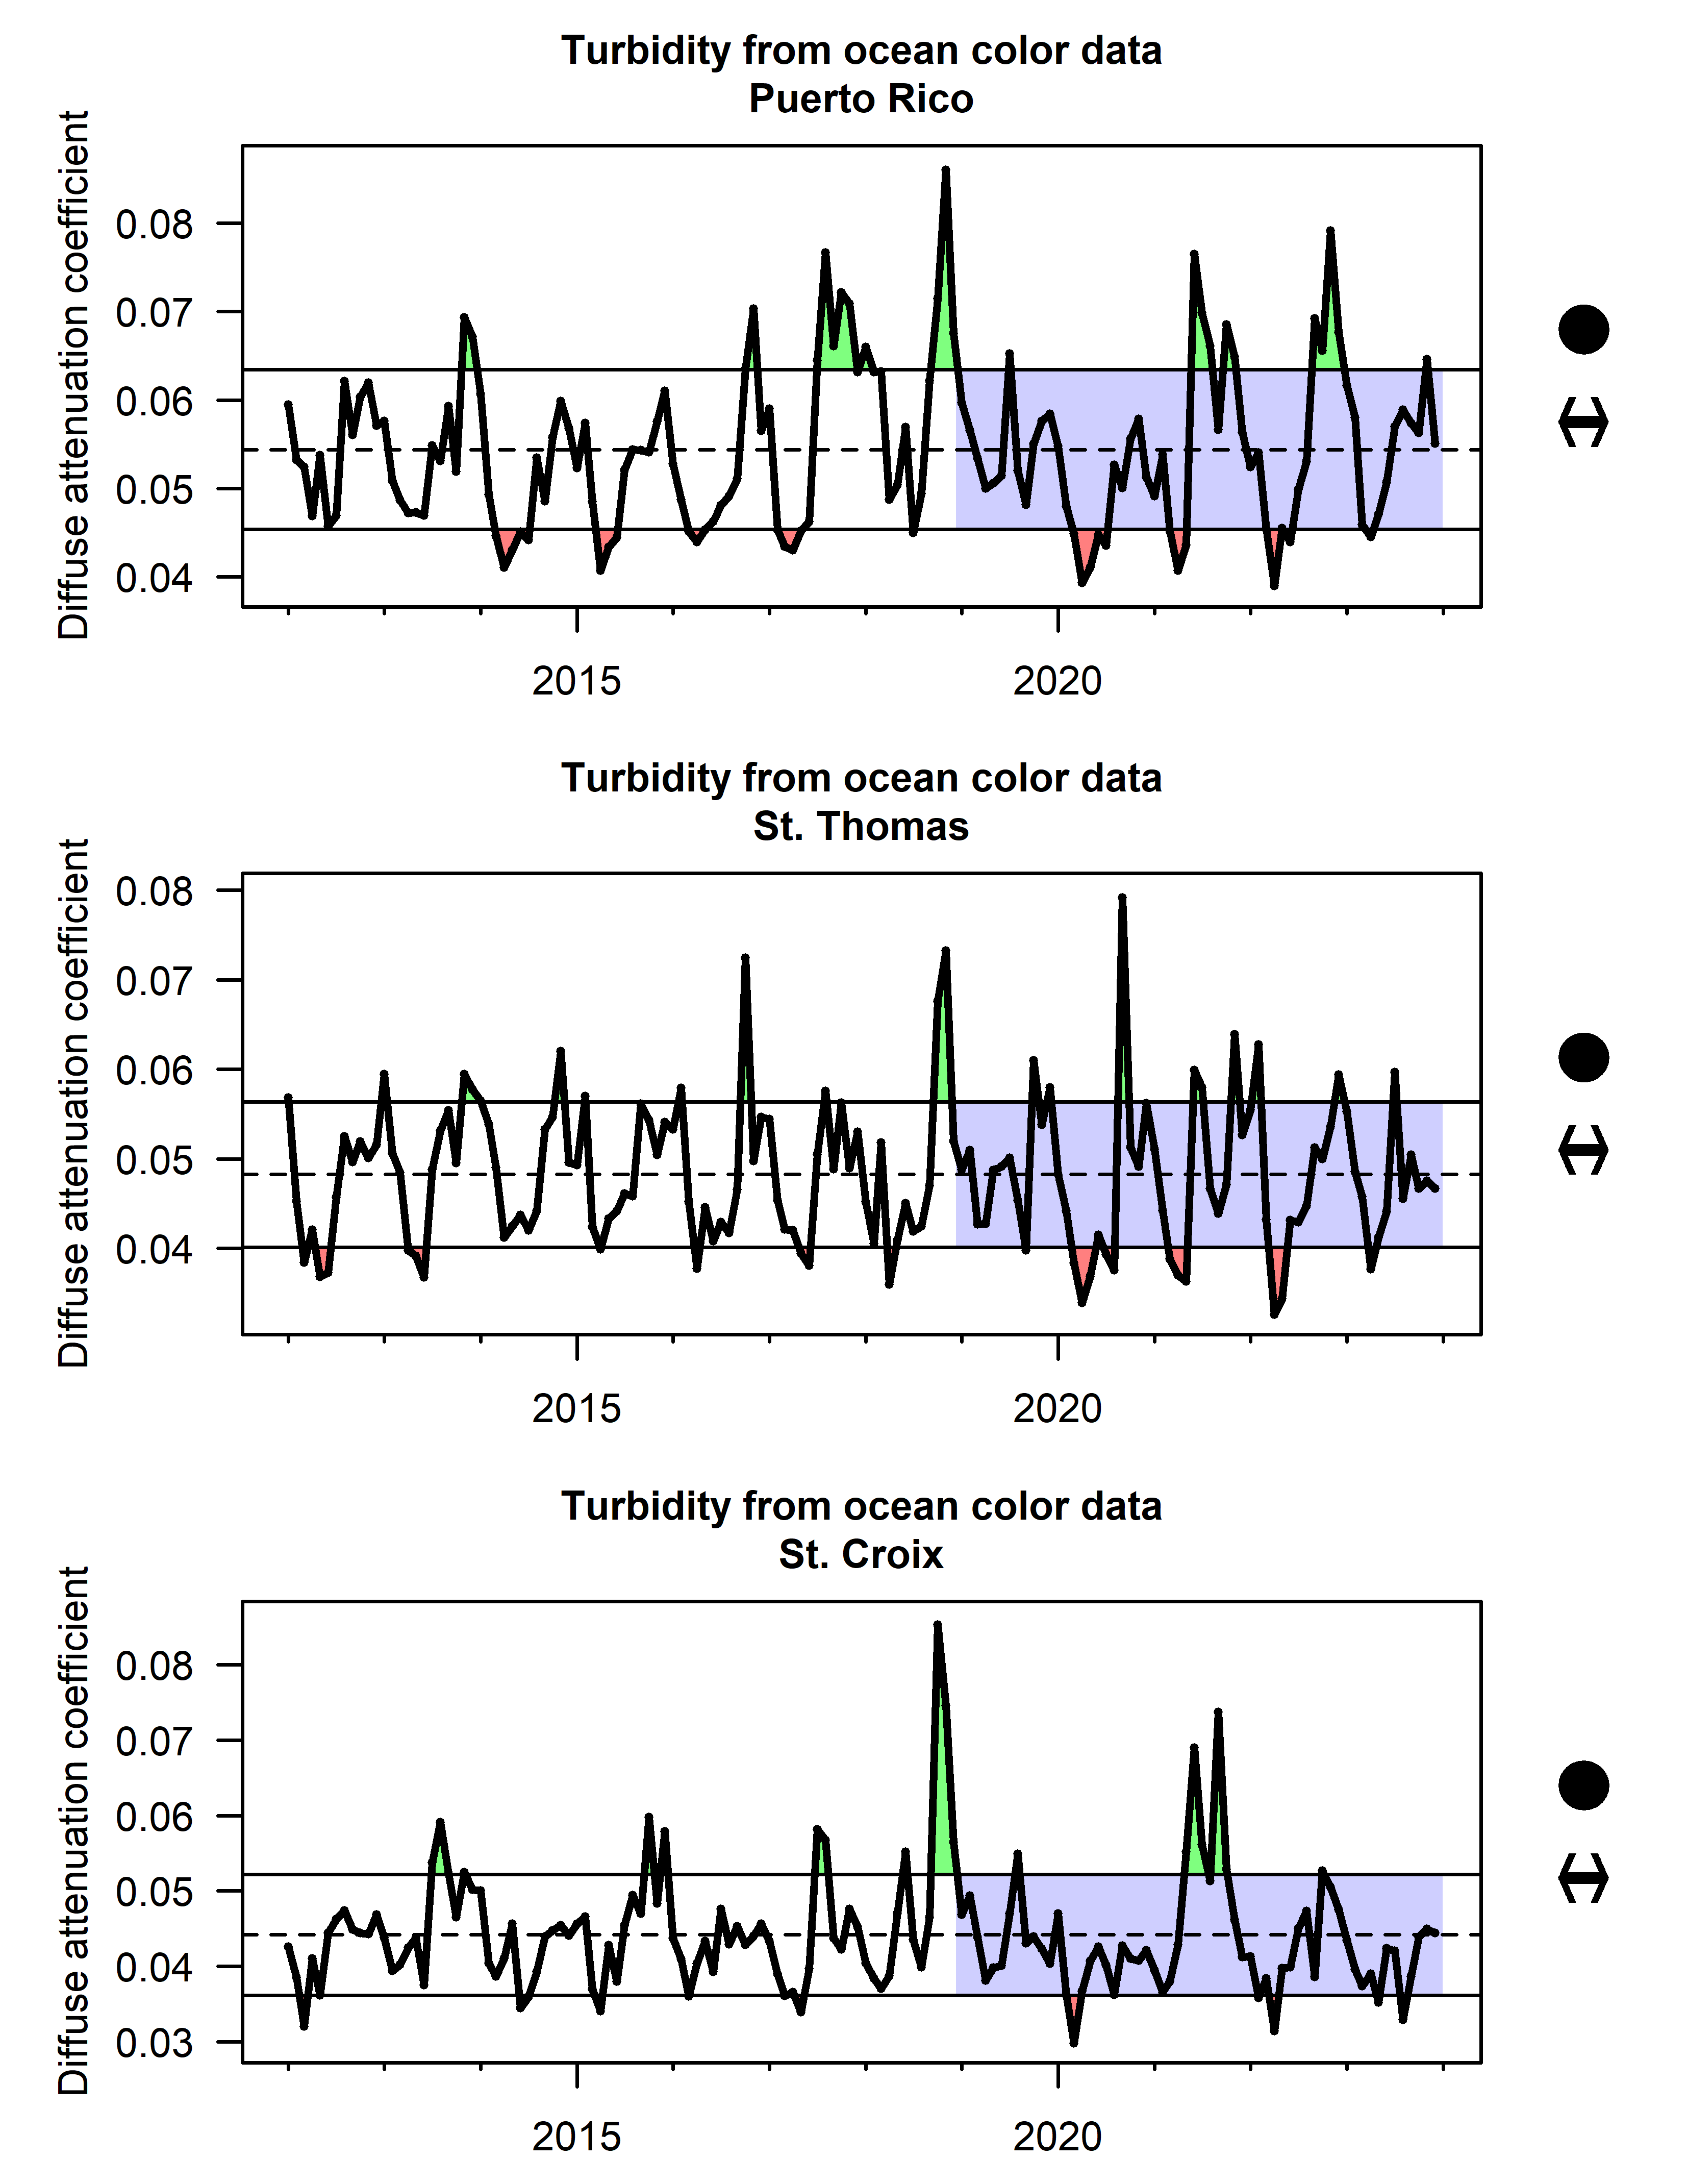
\includegraphics[width=0.75\linewidth,height=\textheight,keepaspectratio]{indicator_plots/turbidity_plot_final.png}

}

\caption{\label{fig-turb}Standardized monthly anomalies of water
turbidity as measured by the diffuse attenuation coefficient, for waters
surrounding Puerto Rico (top), St.~Thomas and St.~John (middle) and
St.~Croix (bottom).}

\end{figure}%

\section{Water quality}\label{water-quality}

The presence of enterococci bacteria in water samples is used as a
primary indicator of fecal contamination, which poses both environmental
and human health risks (United States Environmental Protection Agency
2024). Water quality, biological, and physical data collected by the
USGS, the EPA, and over 400 state, federal, tribal, and local agencies
are publicly available via the EPA Water Quality Portal
(\url{https://www.waterqualitydata.us/}). Data on enterococci abundance
in beach samples throughout Puerto Rico and the USVI were downloaded and
daily counts were averaged annually. Throughout the U.S. Caribbean
region, there has been a substantial increase in the enterococcus count
over time, with particularly high measured levels since 2015 in Puerto
Rico and since 2020 in USVI Figure~\ref{fig-ent}.

\begin{figure}

\centering{

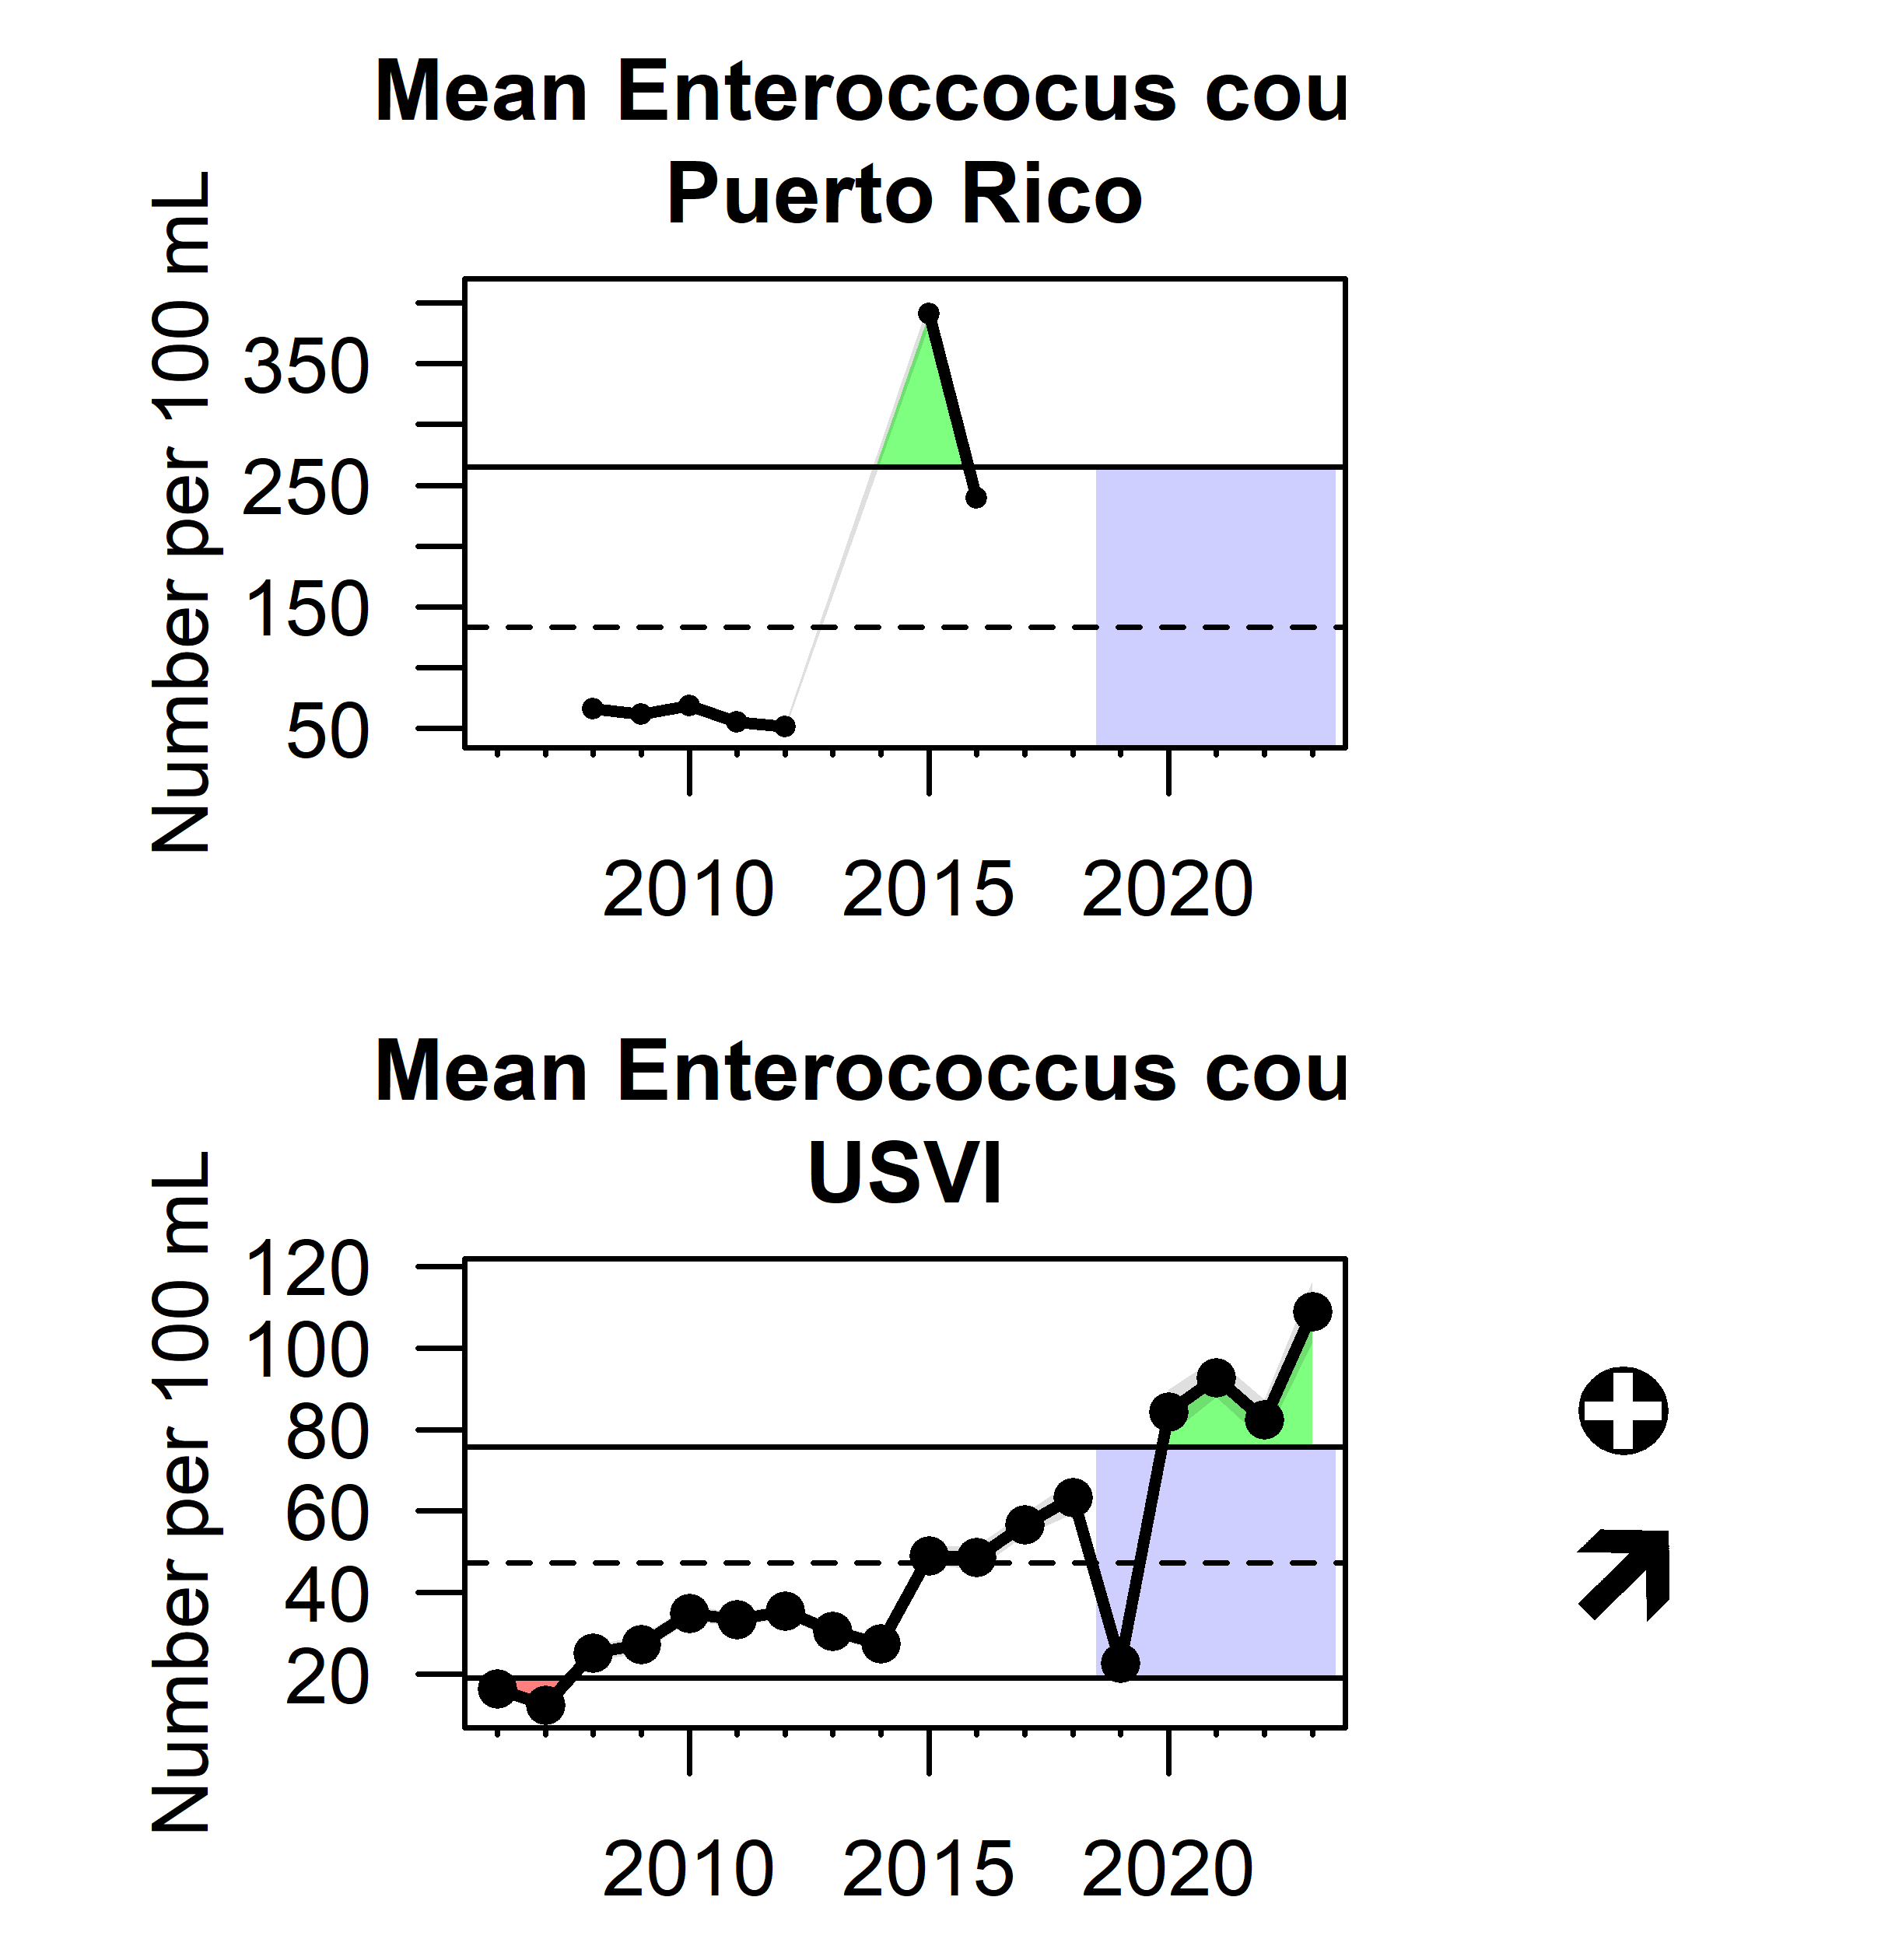
\includegraphics[width=0.75\linewidth,height=\textheight,keepaspectratio]{indicator_plots/enterococcus_plot_final.png}

}

\caption{\label{fig-ent}Water quality as measured by average
enterococcus counts (+/- 1 S.E.) from beach water quality sampling at
sites in Puerto Rico (top) and the USVI (bottom).}

\end{figure}%

\section{Coastal development}\label{coastal-development}

Impervious surfaces such as pavement, sidewalks, roofs and roads, as
well as other forms of development, reduce the infiltration of water
into the ground. Impervious surfaces often contribute to higher storm
water runoff, greater sediment yields into coastal areas, and increased
pollutant loads, all of which can degrade water quality (NOAA Digital
Coast). This indicator influences water quality and turbidity in
nearshore coastal habitat areas. As of 2022, the highest amount of
impervious surfaces is seen in the San Juan metropolitan area
(Figure~\ref{fig-landuse}).

\begin{figure}

\centering{

\pandocbounded{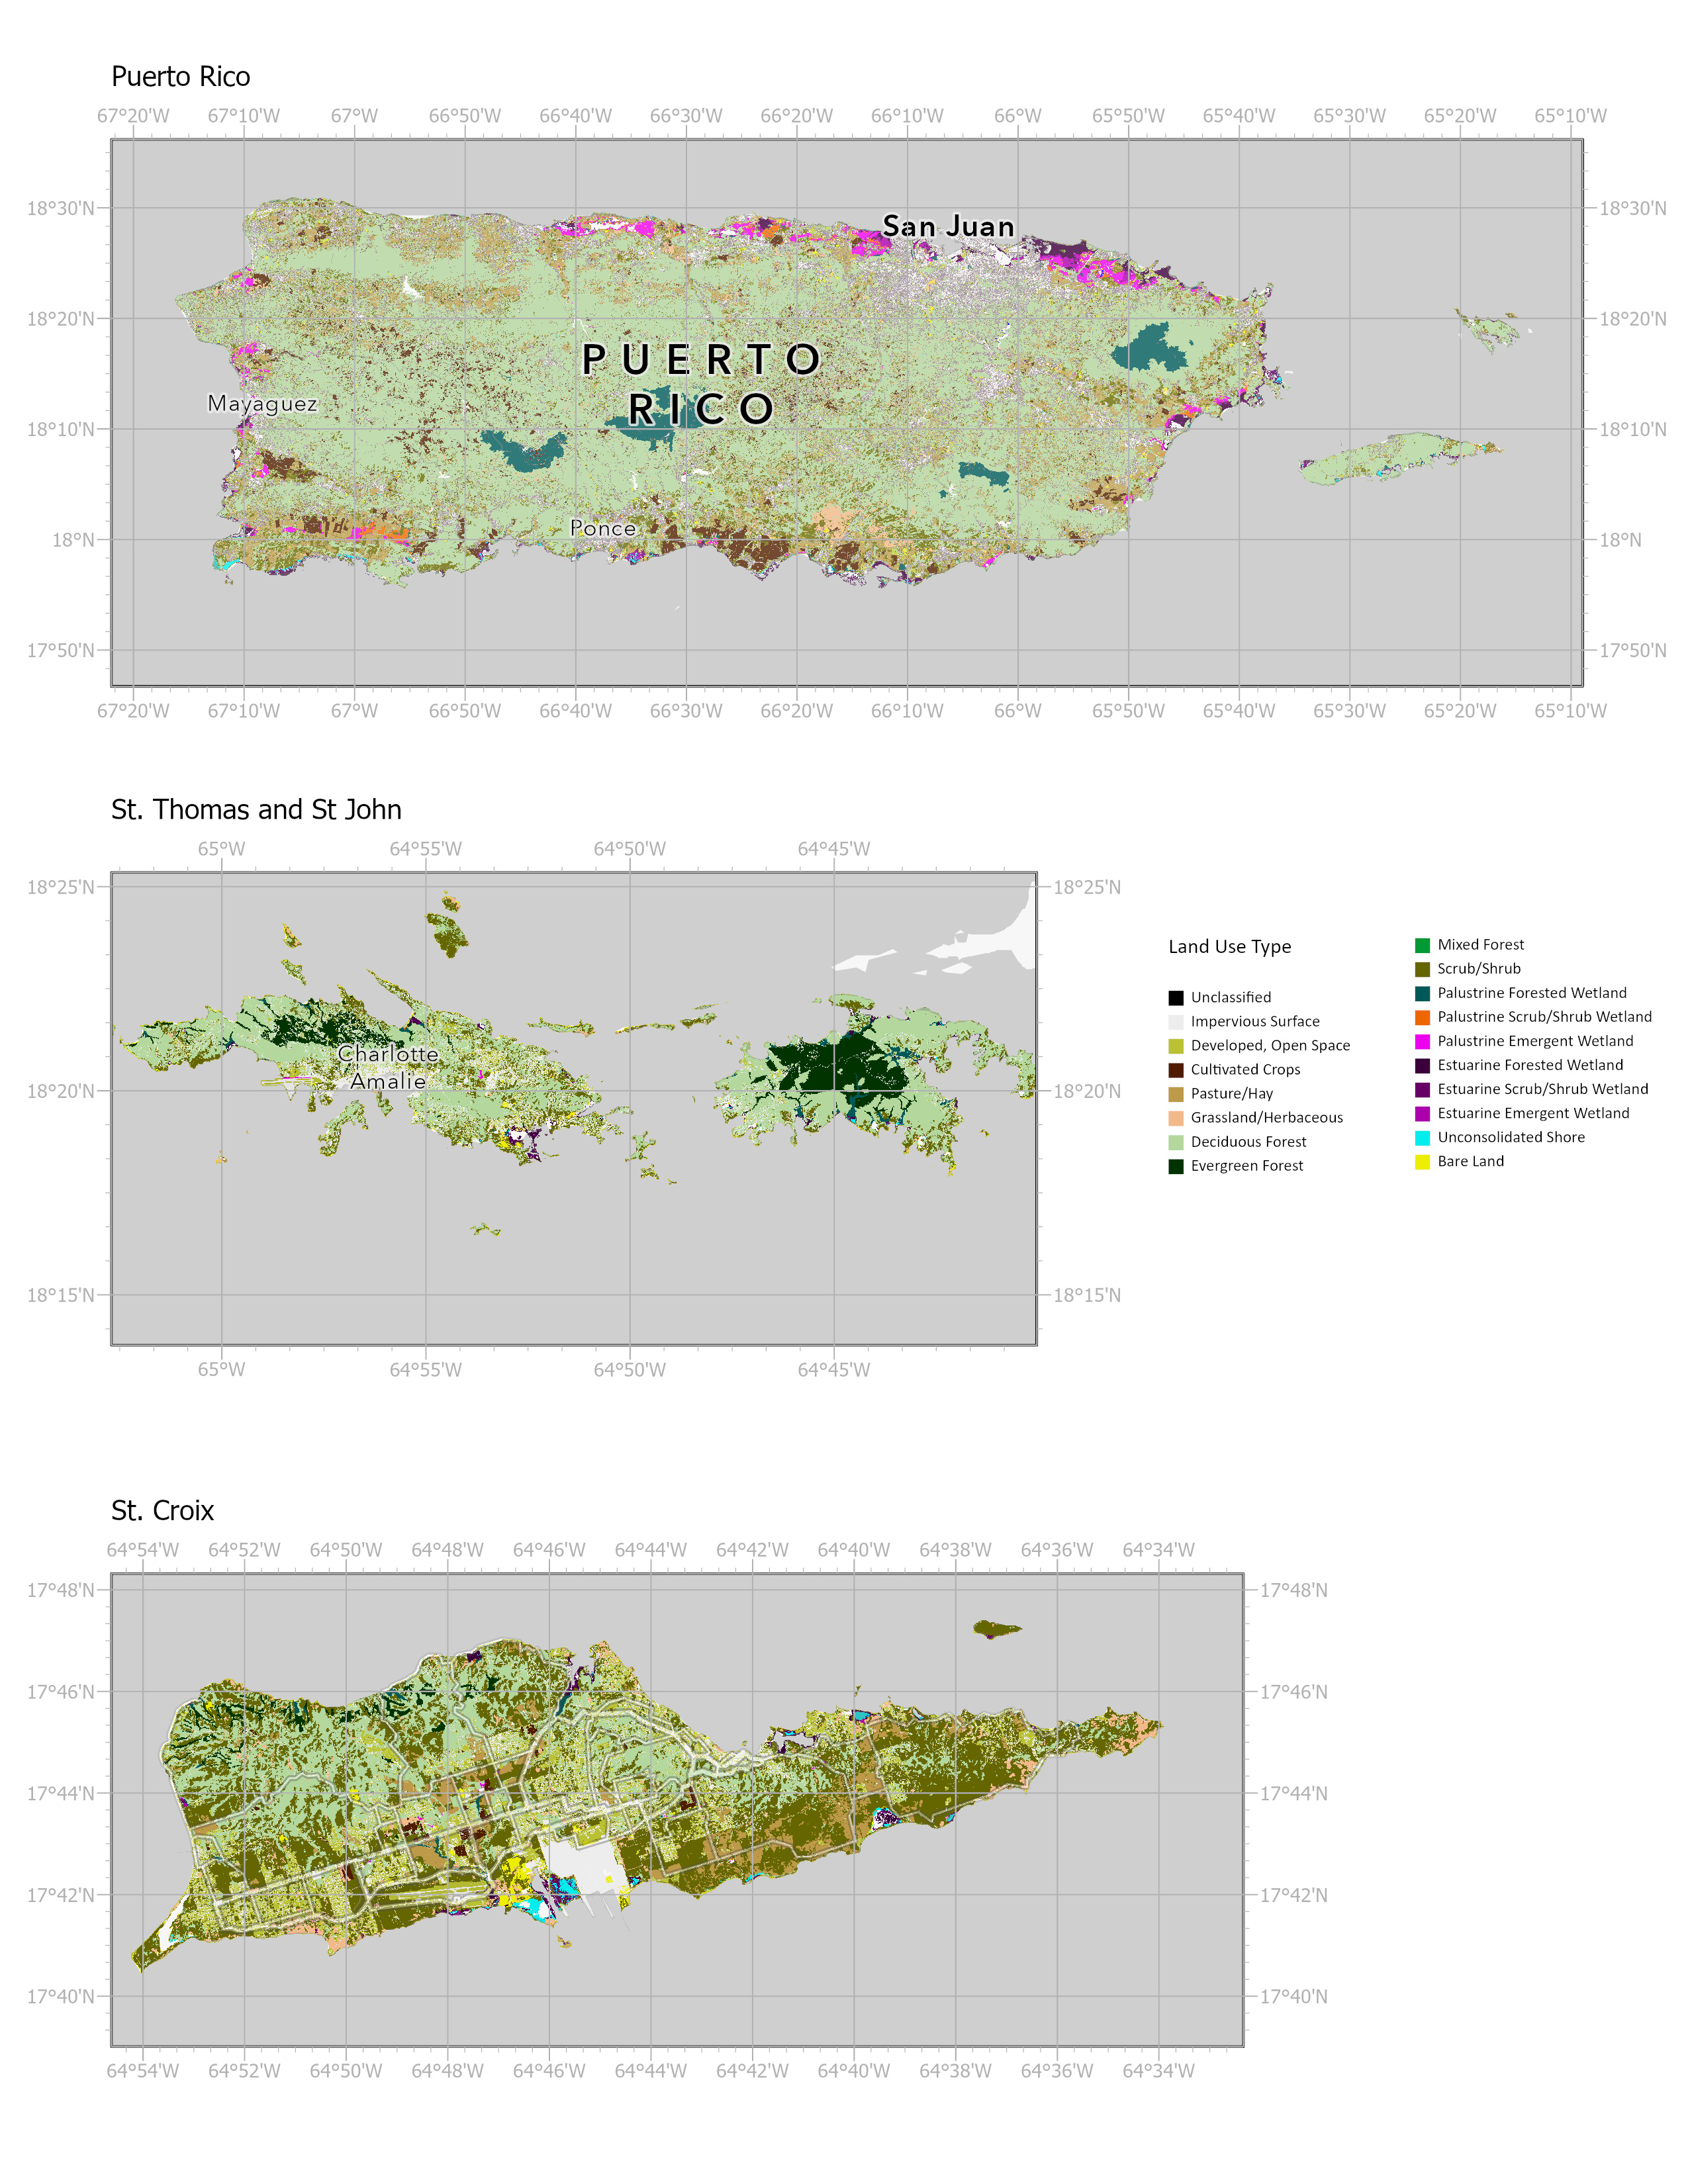
\includegraphics[keepaspectratio]{indicator_plots/Land_Use_Land_Cover_2024.jpg}}

}

\caption{\label{fig-landuse}Impervious surfaces from development in the
U.S. Caribbean.}

\end{figure}%

\section{Primary productivity}\label{primary-productivity}

Primary productivity is a measure of the total energy available in an
ecosystem, and is closely correlated with chlorophyll a concentrations.
Average chlorophyll a concentrations are derived from the European Space
Agency Climate Change Initiative's Ocean Colour product, which provides
a bias-corrected composite of measurements merged from multiple
satellite sensors (Hu, Lee, and Franz 2012). Concentrations are plotted
as standardized monthly anomalies as there is a seasonal signal that
could mask long-term trends. Estimates show a decadal cyclical pattern,
with no overall or recent trend apparent (Figure~\ref{fig-chl}).

\begin{figure}

\centering{

\pandocbounded{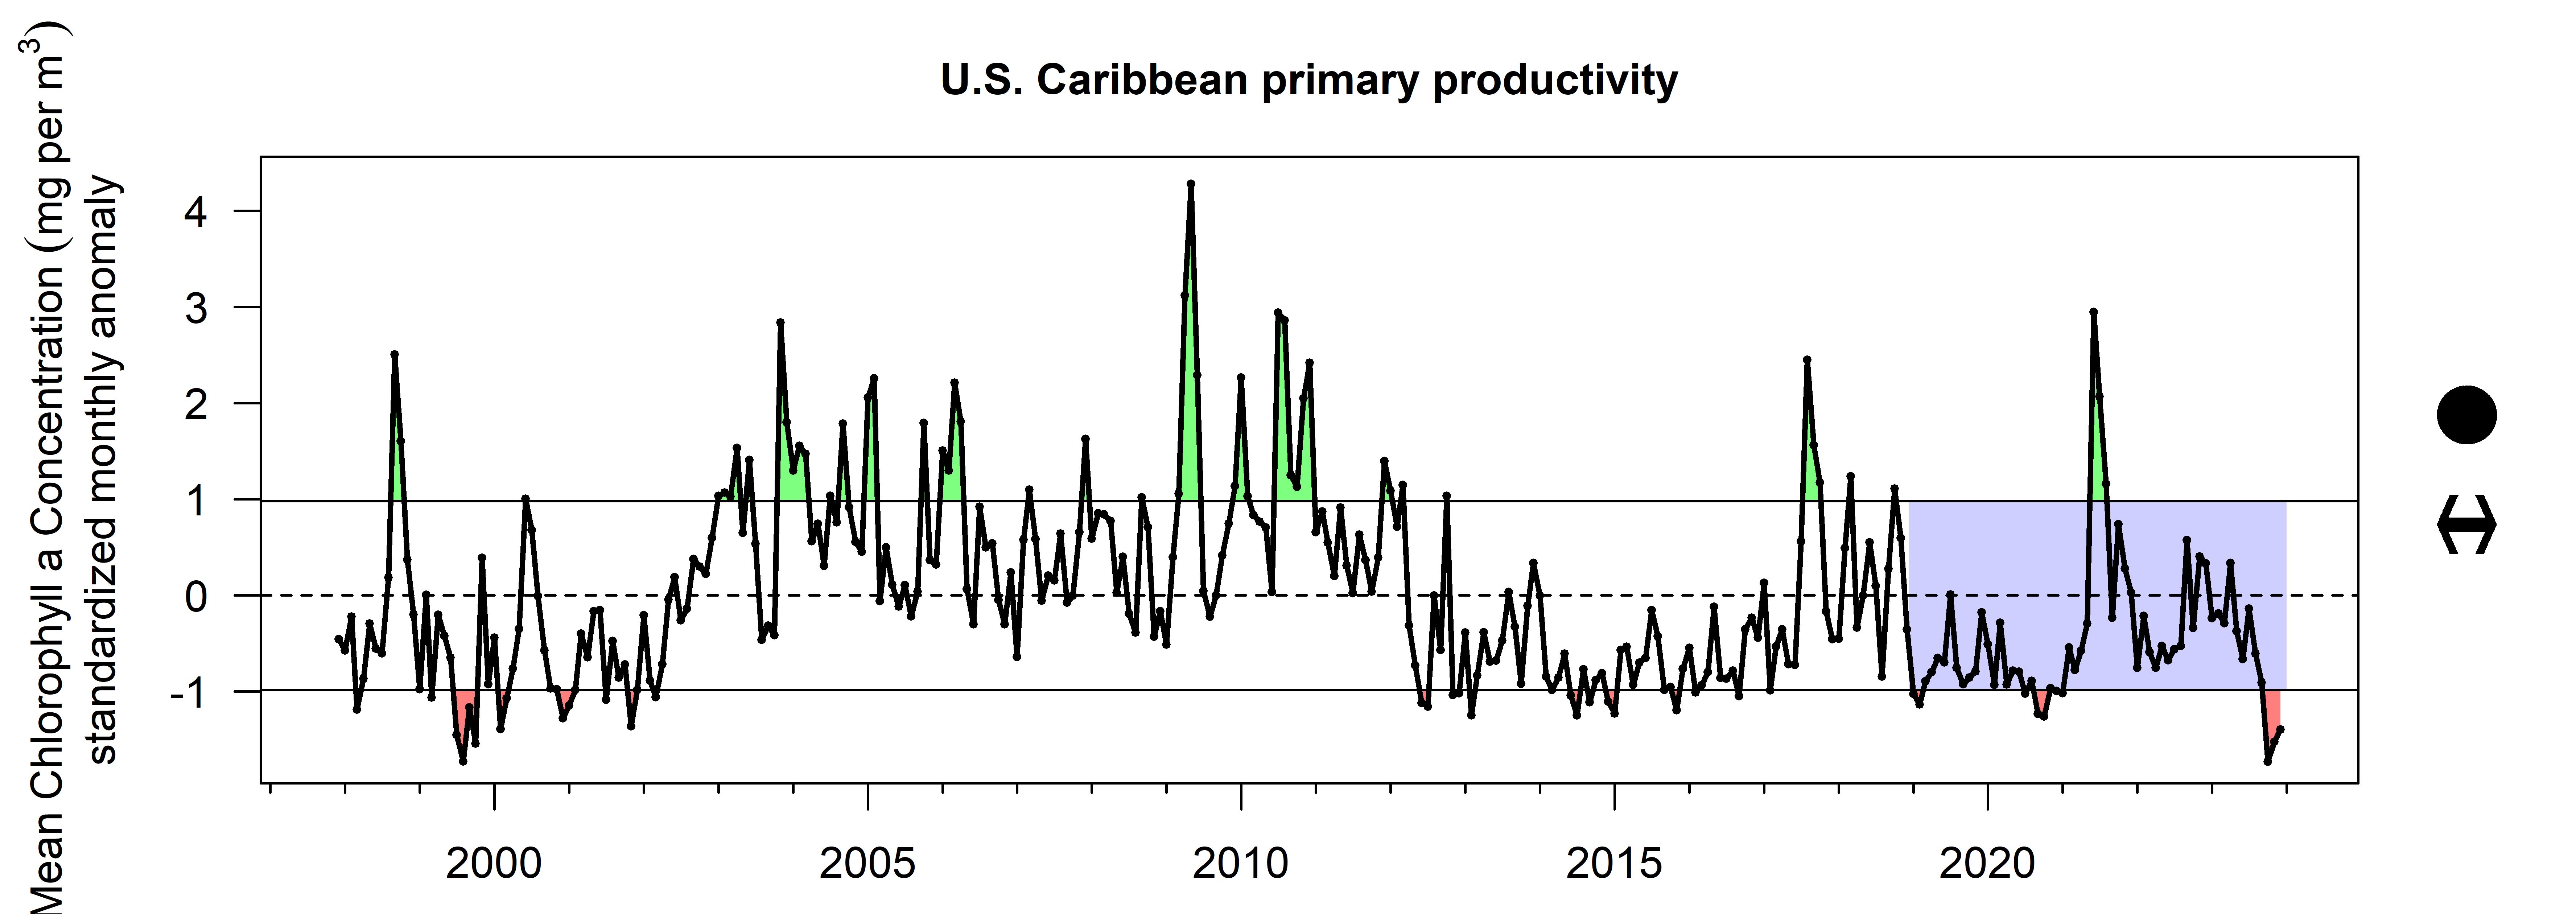
\includegraphics[keepaspectratio]{indicator_plots/carib_Chl_plot_final.png}}

}

\caption{\label{fig-chl}Changes in ocean color showing mean chlorophyll
a levels (standardized monthly anomalies) in the U.S. Caribbean region.}

\end{figure}%

\section{Sargassum inundation}\label{sargassum-inundation}

Sargassum (brown macroalgae \emph{S. fluitains} and \emph{S. natans}) is
a designated essential fish habitat important for many pelagic fish and
protected species; however, when large blooms collect in nearshore
environments they can reduce oxygen, suffocate beaches and have
detrimental impacts on marine species(Hu et al. 2016). Mean monthly
Sargassum wet biomass is estimated from satellite measurements using the
algorithm of Wang et al. (Wang et al. 2019). Sargassum blooms were
largely absent from the U.S. Caribbean prior to 2011, but bloom activity
has been generally increasing since that year (Figure~\ref{fig-sarg}).
Major inundation events occurred in 2018 and 2021.

\begin{figure}

\centering{

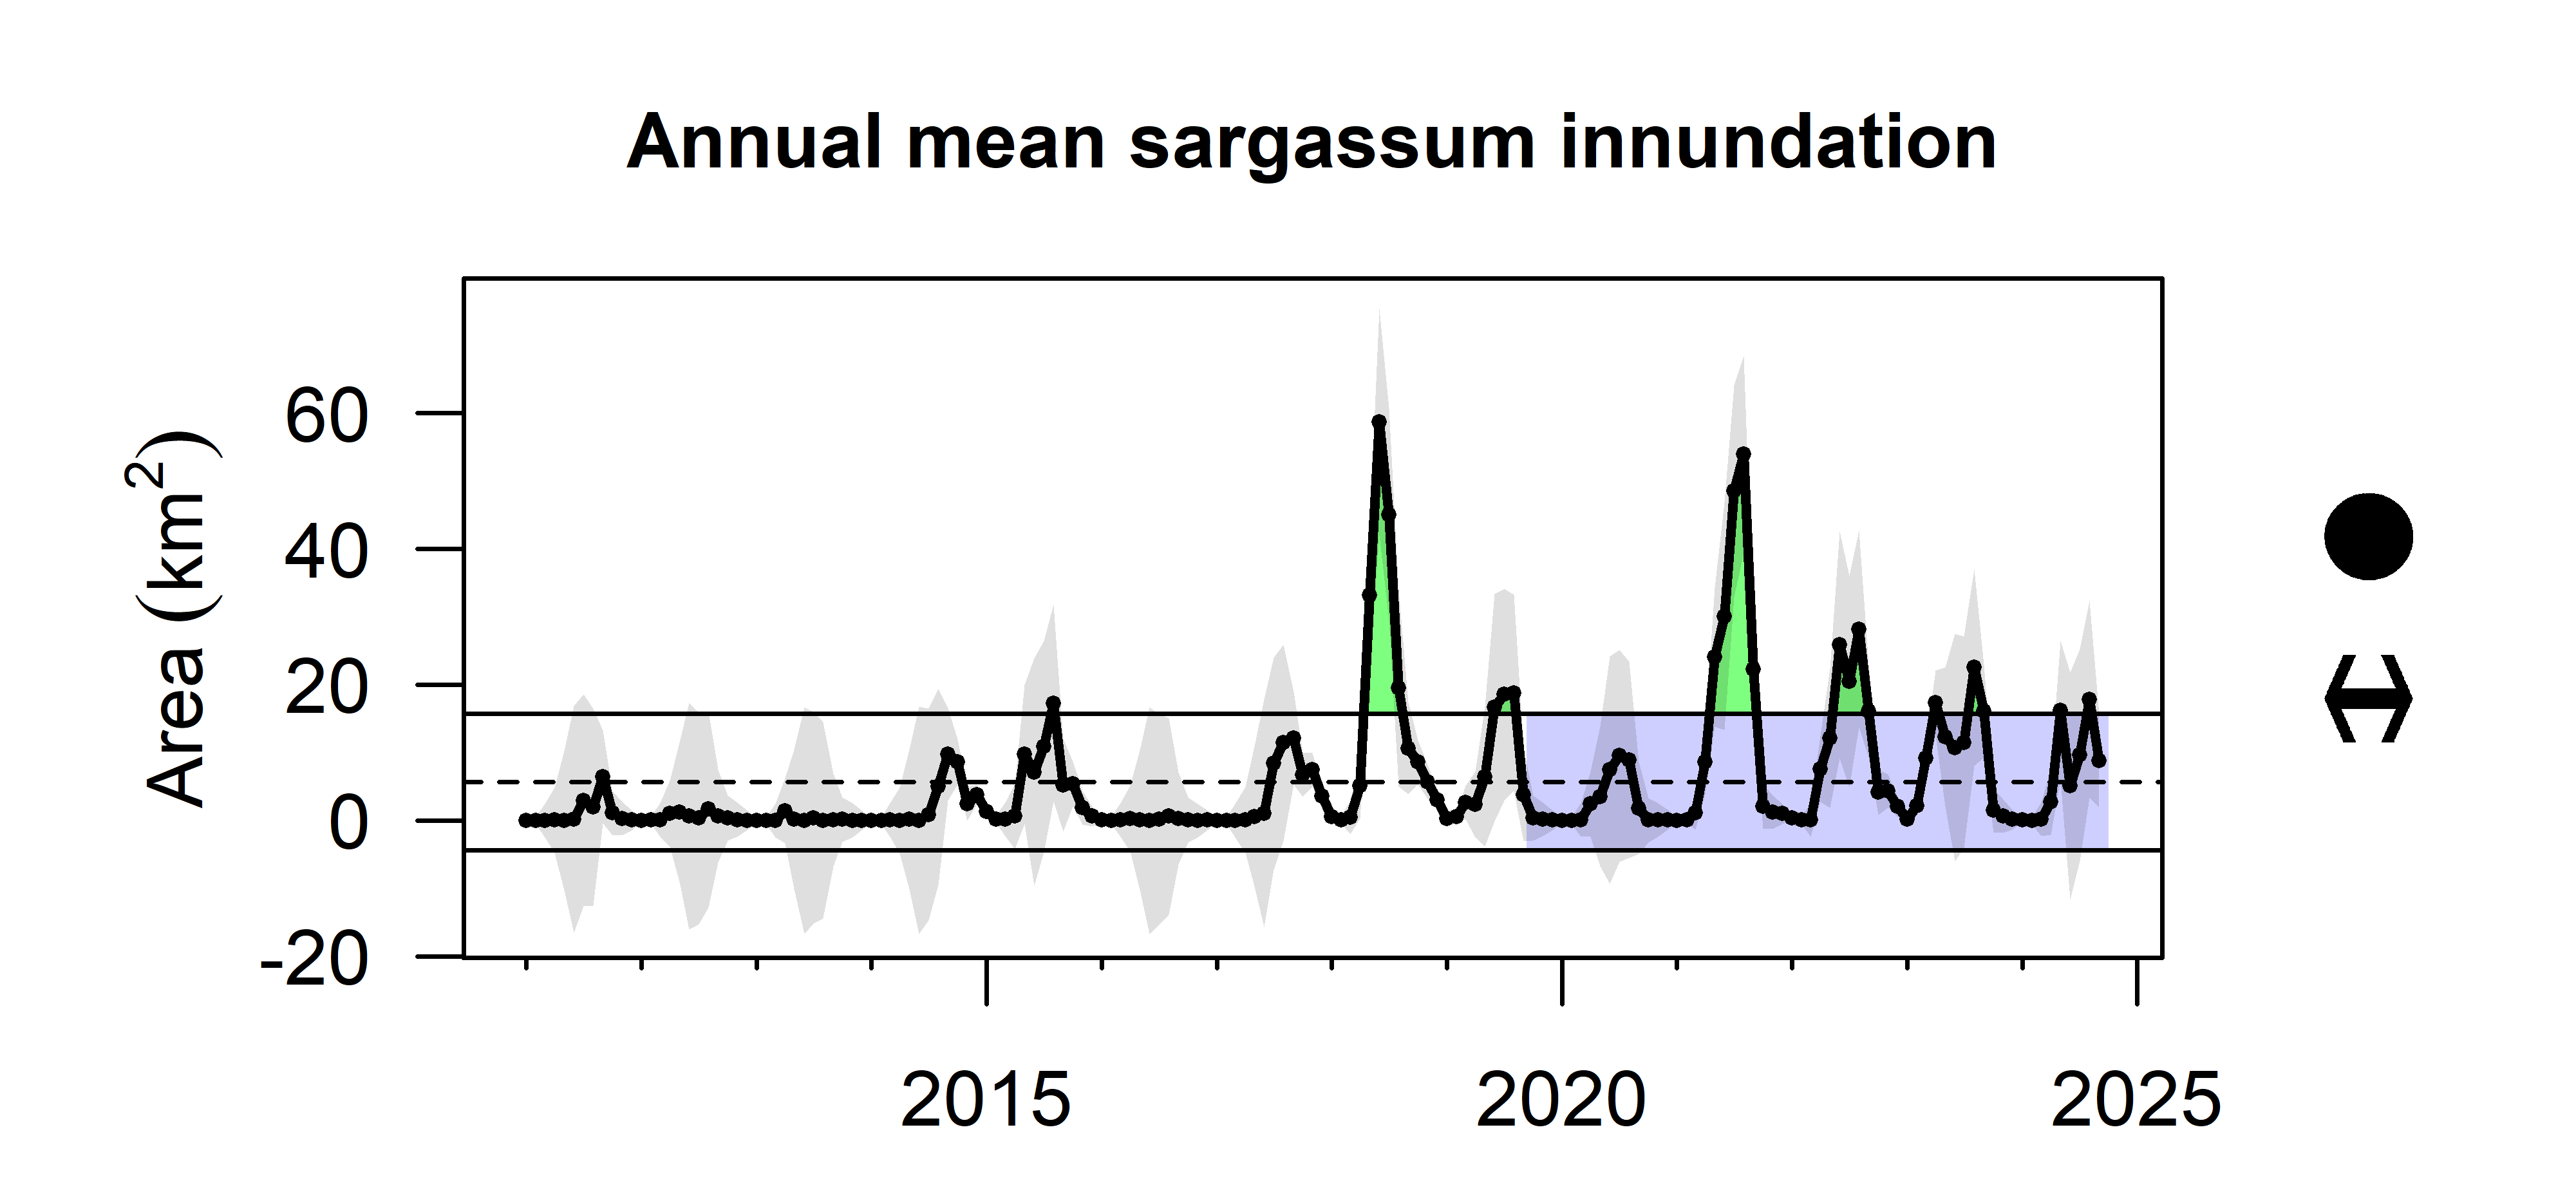
\includegraphics[width=0.75\linewidth,height=\textheight,keepaspectratio]{indicator_plots/Sargassum_plot_final.png}

}

\caption{\label{fig-sarg}Annual mean sargassum inundation in square km
of cover in the U.S. Caribbean.}

\end{figure}%

\section{Market disturbances}\label{market-disturbances}

Alterations to typical fishing patterns can be quantified by analyzing
the seasonality of how fishing activity is distributed throughout the
year and detecting deviations from average patterns. A market
disturbance indicator was developed by calculating the proportion of
landings in each month of the year, and summing the square of deviations
between those monthly proportions from the mean proportions across all
years:

\(D_y = \sum_{m=1}^{12} (P_{m,y} - \overline{P}_m)^2\)

This calculation was carried out for the species with highest landings
that have not been subject to seasonal closures; the mean and standard
deviation are calculated for the disturbance indicator across those
species. In Puerto Rico, there is little trend in the disturbance
indicator; however there were higher disturbance indicator values in
2005 and 2017. In St.~Thomas, the indicator increases throughout time
and detects a major disturbance in the 2017--2018 fishing season (i.e.,
July 1st 2017 to June 30th 2018). In St.~Croix, disturbance levels were
high in 2017--2018 and also 2019--2020 (Figure~\ref{fig-dist}).

\begin{figure}

\centering{

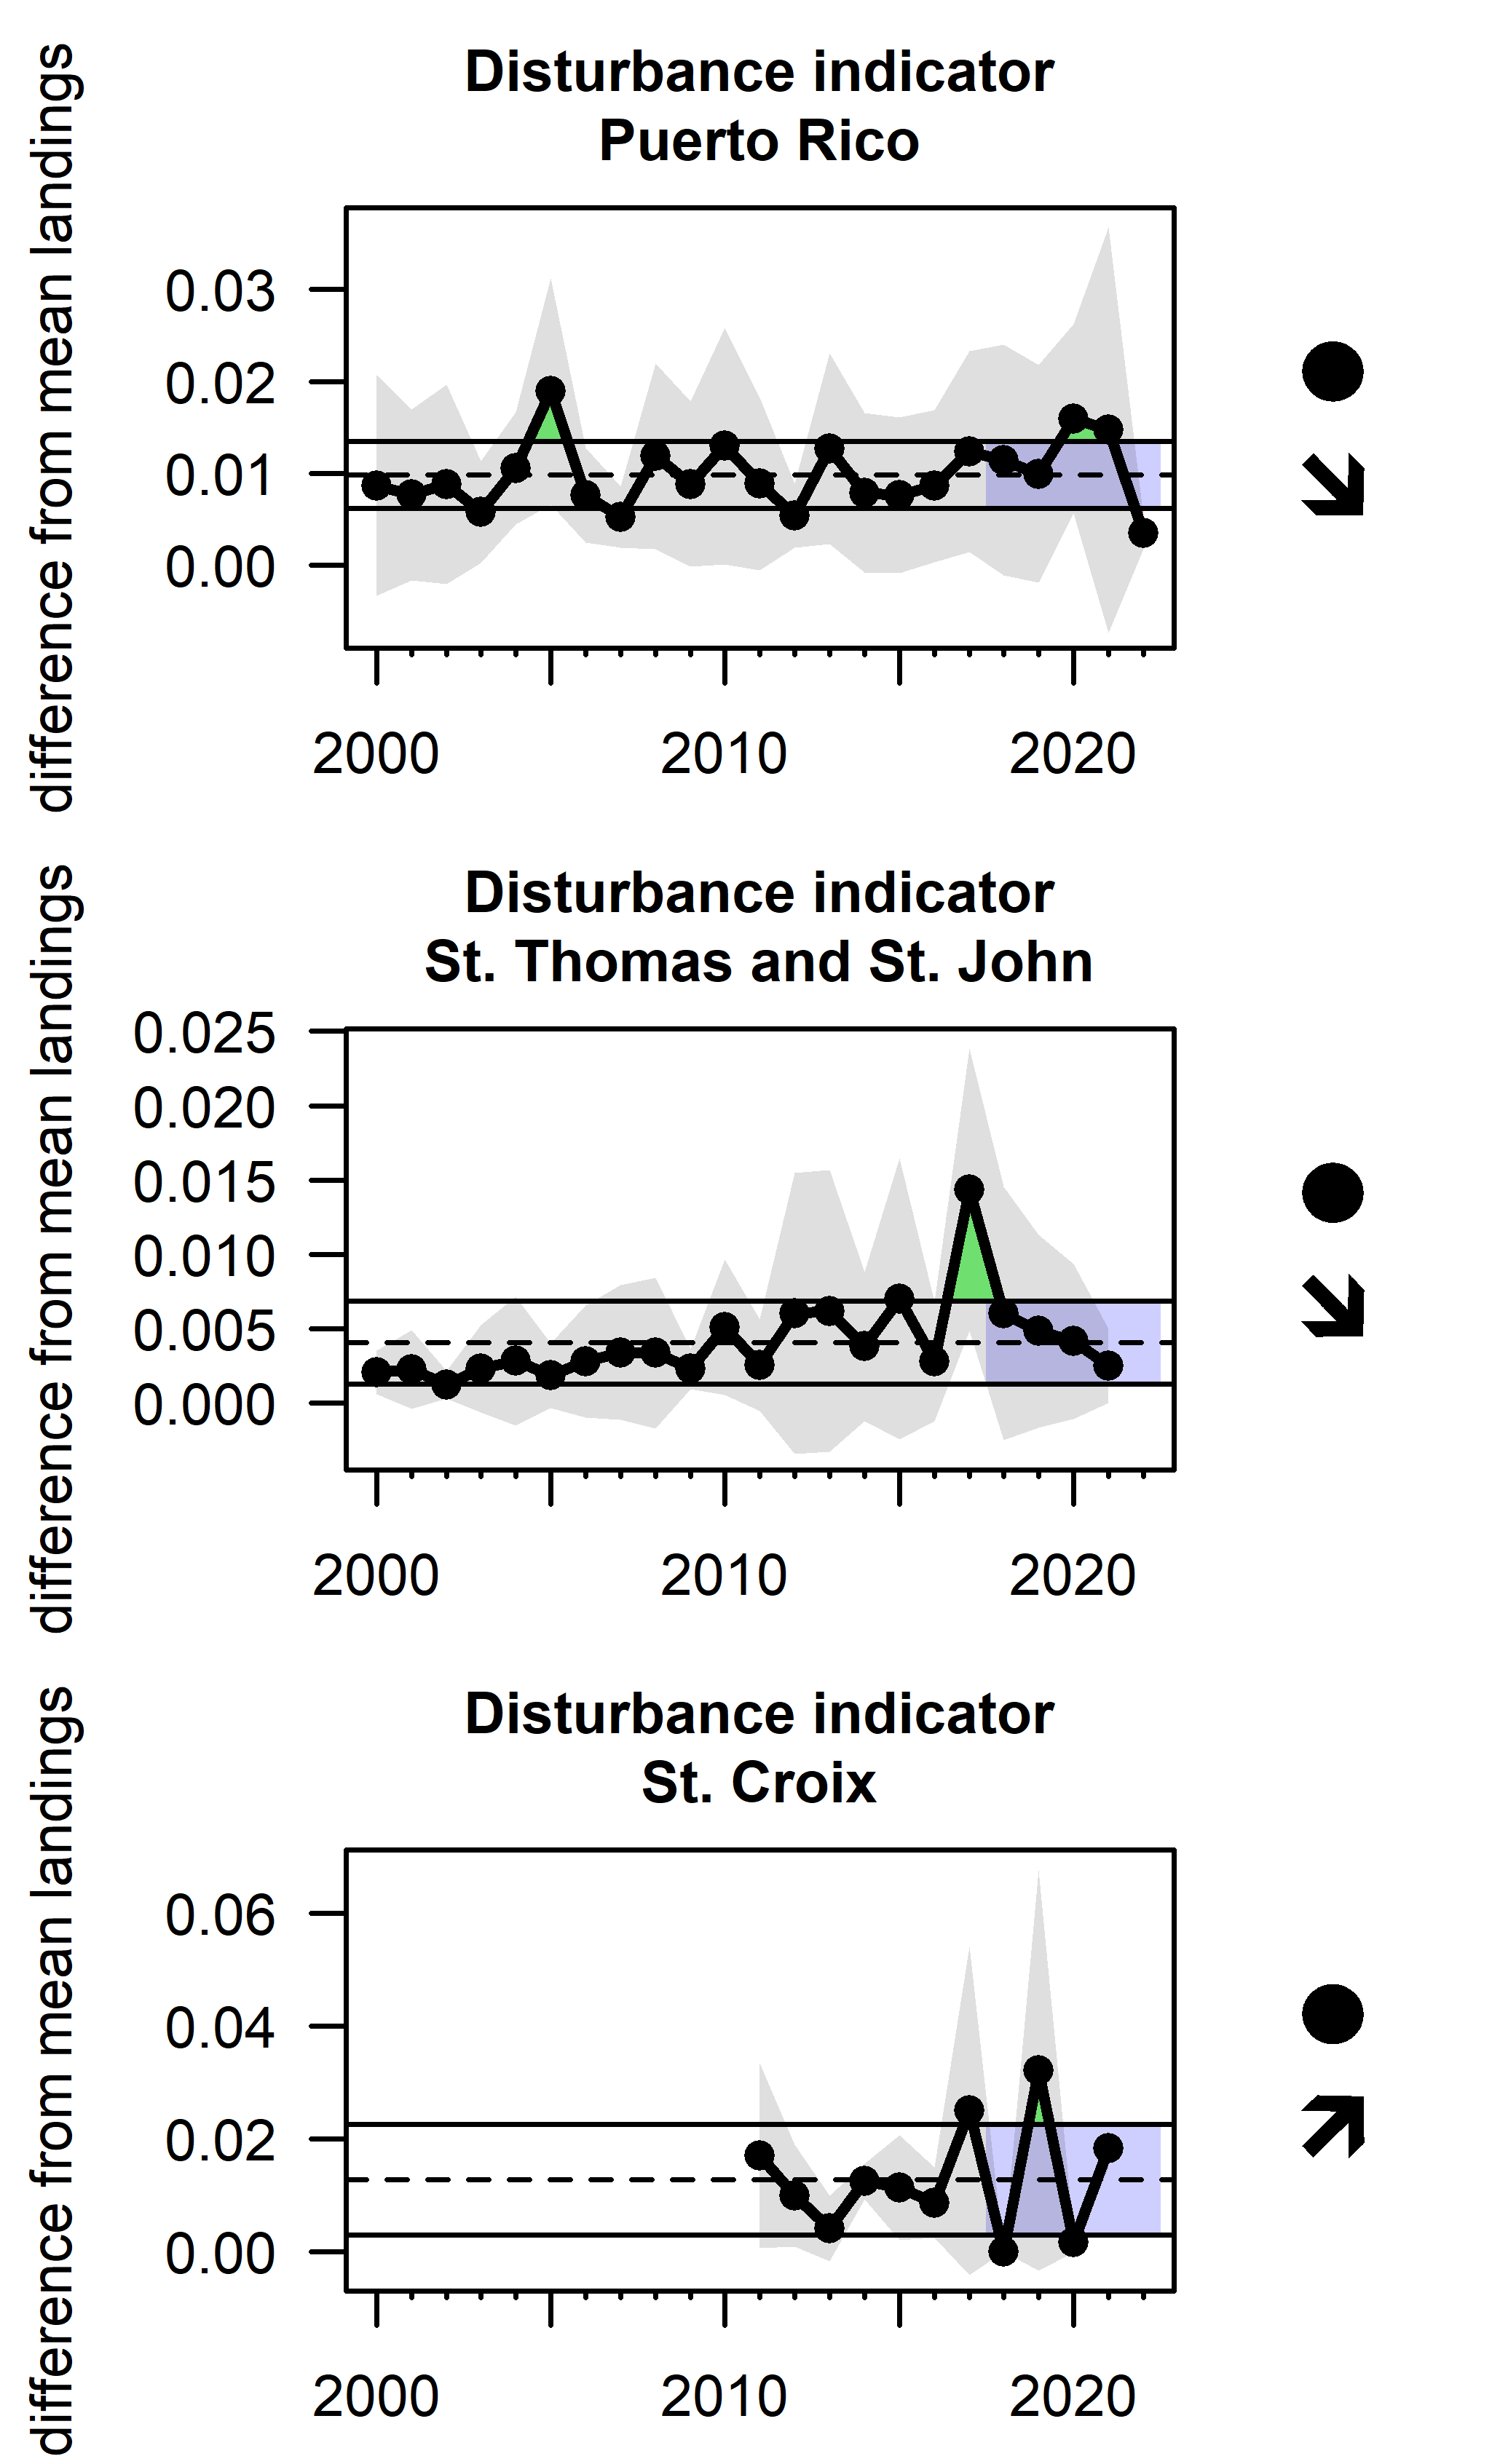
\includegraphics[width=0.75\linewidth,height=\textheight,keepaspectratio]{indicator_plots/disturbance_plot_final.png}

}

\caption{\label{fig-dist}Disturbance level (+/- 1 S.D.), calculated as
the departure from mean seasonal landings patterns for top species in
Puerto Rico (top), St.~Thomas and St.~John (middle) and St.~Croix
(bottom). Note that the years in the USVI are fishing years (July 1st to
June 30th of the following year).}

\end{figure}%

\section{Human activity}\label{human-activity}

Human activity has an impact on the marine ecosystem indirectly through
its influence on coastal development and pollution, as well as directly
through marine tourism, fishing and demand for seafood. Human activity
is exerted by the local population as well as the extensive tourism
industry that exists in the U.S. Caribbean. Total population estimates
are reported by the U.S. Census Bureau and tourism activity can be
measured through hotel occupancy rates (data from the Puerto Rico
Tourism Company and USVI Bureau of Economic Research) and the number of
air and cruise passengers (data from the Puerto Rico Ports Authority and
USVI Bureau of Economic Research). Human population in the U.S.
Caribbean has been declining gradually since 2000
(Figure~\ref{fig-pop}). Tourism has fluctuated over time, with major
decreases in air and cruise passengers 2017 and 2020, but recovery to
normal or above-normal levels since (Figure~\ref{fig-tourist}). A
similar decline in hotel registrations in 2020 is apparent in the Puerto
Rico data, following a general recovery. The total hotel guest count in
USVI however declined in 2018 and has not recovered, though this is
likely driven in part by a rise in vacation property rentals
(Figure~\ref{fig-hotel}).

\begin{figure}

\centering{

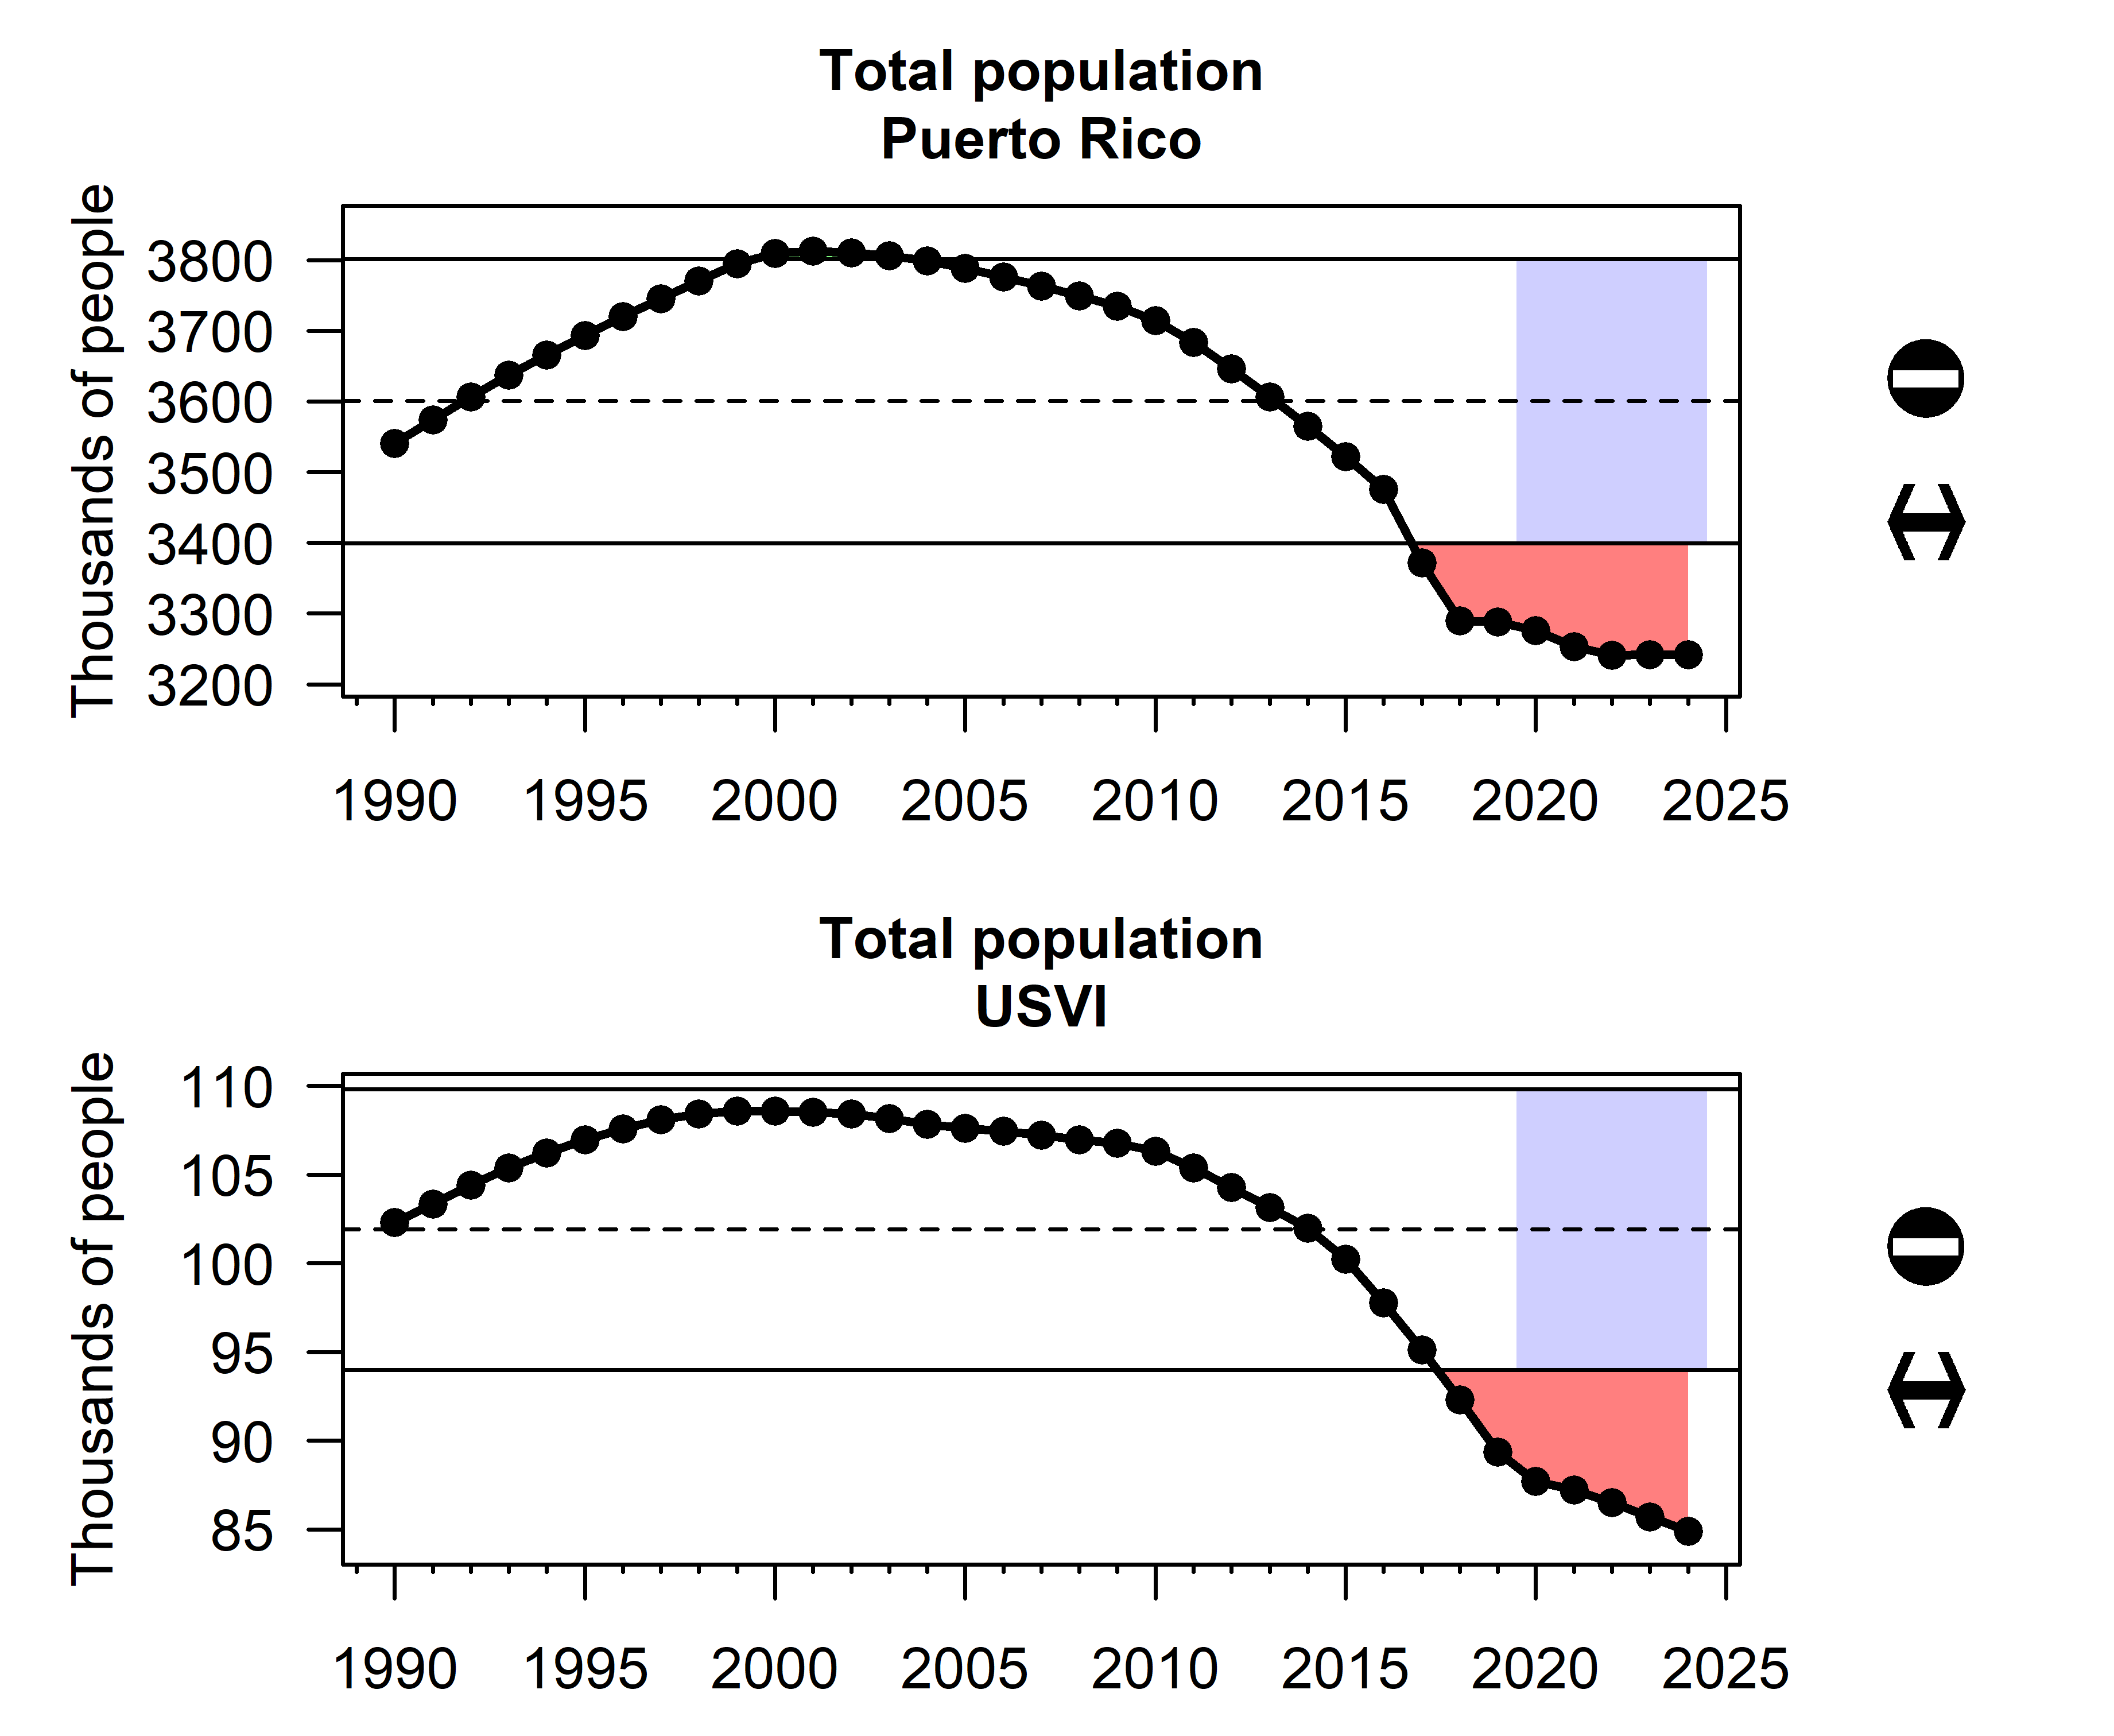
\includegraphics[width=0.75\linewidth,height=\textheight,keepaspectratio]{indicator_plots/population_plot_final.png}

}

\caption{\label{fig-pop}Population change in Puerto Rico (top) and USVI
(bottom) according to census data.}

\end{figure}%

\begin{figure}

\centering{

\pandocbounded{\includegraphics[keepaspectratio]{indicator_plots/cruise_plot_final.png}}

}

\caption{\label{fig-tourist}Annual tourism activity in Puerto Rico
(left) and USVI (right) as indicated by the number of cruise and air
passengers visiting the islands.}

\end{figure}%

\begin{figure}

\centering{

\includegraphics[width=0.75\linewidth,height=\textheight,keepaspectratio]{indicator_plots/hotel_plot_final.png}

}

\caption{\label{fig-hotel}Annual tourism activity in Puerto Rico and
USVI as indicated by the number of hotel registrations (guests). Note
that Puerto Rico data only include non-resident hotel registrations
while for USVI data were available for all hotel registrations, so may
include residents and non-residents.}

\end{figure}%

\bookmarksetup{startatroot}

\chapter{Integrated ecosystem
perspectives}\label{integrated-ecosystem-perspectives}

\section*{}\label{section}
\addcontentsline{toc}{section}{}

\markright{}

For the purpose of synthesizing the information contained in the full
suite of indicators presented in this report, we analyze the full
indicator suite using multivariate methods. Principal components
analysis (PCA) is a statistical method that distills a large number of
potentially related indicators into a smaller number of indices
representing most of the variability in the data set. We analyze the
indicator suite separately by category: 1) risks to meeting management
objectives, 2) management objective indicators based on
fishery-independent data, 3) management objective indicators based on
fishery-dependent data, and 4) other management objective indicators. A
traffic light plot of the indicator suite is presented for the purpose
of comprehensively viewing changes in the different parts of the
ecosystem over time (Figure~\ref{fig-traffic}). A biplot of the
principal components analysis is presented to convey temporal patterns
in the progression of ecosystem status (Figure~\ref{fig-PCA}). PCA was
carried out on a scaled matrix for all indicators with at least 12 years
of data; any missing values were imputed with means of the time series.
In the biplot, the labels represent time (years 2011 -- 2023), the
rainbow line represents chronology between adjacent years, and the
distance between points conveys how different the indicator values were
in those years.

\begin{figure}

\centering{

\includegraphics[width=1\linewidth,height=\textheight,keepaspectratio]{indicator_plots/traffic.png}

}

\caption{\label{fig-traffic}Traffic light plot representing the value of
the indicator each year according to quintiles; colors show that the
indicator moving between well below average (red, bottom quintile),
below average (orange, 20-40\% quintile), average (yellow, 40-60\%
quintile), above average (light blue, 60-80\% quintile), and well above
average (dark blue, top quintile), respectively (see legend). Indicators
are grouped by category, and appear on the plot sorted by their loading
(i.e., their influence) from a principal components analysis. In this
way, indicators showing similar patterns across time are grouped more
closely together.}

\end{figure}%

\begin{figure}

\centering{

\includegraphics[width=1\linewidth,height=\textheight,keepaspectratio]{indicator_plots/pcas.png}

}

\caption{\label{fig-PCA}Left: Yearly scores of the first two components
of a principal components analysis (PCA) for three groups of indicators,
based on indicator values from 2011 -- 2023. Right: Loadings plots show
the relative influence of each indicator in driving the temporal trends
observed on the left panel. Loadings with an absolute value greater than
0.2 are considered to be significant.}

\end{figure}%

Many indicators are based on time series of limited extent or contain
data gaps, which makes it challenging to elucidate overall trends.
However, the traffic plot conveys that many indicator values undergo
rapid change in the period 2017-2021, and the PCA biplots confirm these
patterns as there are larger two-dimensional shifts between these years.
These shifts are most likely driven by several major stressor events in
this time period, including the major hurricanes Maria and Irma (2017)
and the COVID pandemic (2020-2021). Together, the multivariate analyses
suggest that these events have had some destabilizing impacts on the
U.S. Caribbean fishery ecosystem.

\bookmarksetup{startatroot}

\chapter{Research recommendations}\label{research-recommendations}

\section{Risks to meeting management
objectives}\label{risks-to-meeting-management-objectives}

A number of stressors were identified throughout the conceptual modeling
stage (Seara) and indicator vetting process; however, consistent
monitoring efforts are lacking with which to capture some of these
potential impacts. For example, marine debris was identified as a major
concern, but we could not find any databases reporting standardized
long-term trends in marine debris. Point source pollution, derelict
vessels, and other impacts to water quality are also concerns that are
not well documented in quantitative terms. Coastal development, beach
erosion and their impacts on habitat loss were also a concern,
particularly with respect to nursery habitats such as mangroves and
seagrasses. The NOAA Office for Coastal Management's Coastal Change
Analysis Program is currently in the process of updating its
remotely-sensed imagery of land cover for the U.S. Caribbean; this data
set will allow quantification of habitat and land use changes and can be
included in future iterations of the report.

\section{Fishery-dependent and fishery-independent data
sources}\label{fishery-dependent-and-fishery-independent-data-sources}

Many of the indicators in this report are based on the self-reported
logbook data known as the Caribbean Commercial Logbook (CCL). Logbook
reporting began in 1974; however, reporting forms have changed
throughout the years and catches have been reported at different
taxonomic resolution, typically at family levels in the earlier years
and at the species level only in the last decade. This makes it
challenging to disentangle true signals in the indicators from changing
fishing behavior from artifacts due to changes in reporting. The recent
addition of an electronic reporting option in Puerto Rico is potentially
particularly problematic, as the number of species being reported in the
e-reporting has decreased dramatically relative to paper logbook
reporting, likely due to fatigue in repeating reporting steps for each
new species caught. Further work needs to be conducted to understand how
the various changes in reporting forms have affected landings reports,
and the influence of these reporting artifacts on the trends represented
by indicators.

Additionally, there is high uncertainty surrounding some of the landings
estimates, and underreporting is suspected. A significant decline in
commercial landings occurred in many species around 2010, aligned with
the period when many annual catch limits were initially put into place
in the U.S. Caribbean, and it is thought that reporting may have been
reduced in response to the catch limits out of concern that further
restrictions might be put into place. In Puerto Rico, expansion factors
are used and were applied to the indicators in this report, to account
for known underestimates of commercial landings based on the incoming
reports. These expansion factors, however, are not intended to correct
for the absence of reporting across the island. Because of the issues
and potential biases surrounding the self-reported commercial landings
data, some of the indicators may not accurately reflect true changes in
the fisheries. The indicators based on ratios or percentages (e.g.,
pelagic to demersal ratio, percentage of trips using a certain gear
type) will be less subject to biases related to underreporting, assuming
that the trips that are reported are representative of the overall
fishery. There is currently no regular reporting system for recreational
landings, and this also remains a major source of uncertainty in the
total landings estimates.

Due to the inherent uncertainties and potential biases in self-reported
landings data, interpretation of fishery-dependent data is facilitated
by comparison of trends from standardized fishery-independent data
sources. The Puerto Rico Long-Term Coral Reef Monitoring Program
(PRCRMP) and the USVI Territorial Coral Reef Monitoring Program (TCRMP)
have conducted annual surveys of fish and benthic organisms since the
late 1990s, providing a relatively long-term data set with which to
analyze trends. However, these surveys are conducted at fixed sites at
known locations with good habitat conditions, so may not be
representative of wider regional trends in the populations. The National
Coral Reef Monitoring Program (NCRMP), on the other hand, employs a
stratified random sampling design, which better accounts for the variety
of habitat types in the region; however, sampling is conducted every
other year. Some preliminary explorations of these data sets were
explored in this report, but could be mined for more signals. In
particular, community-level and/or length-based indicators could be
informative for understanding the response of populations and fish
communities to fishing and other drivers.

\section{Human dimensions}\label{human-dimensions}

From the perspective of human well-being as it relates to marine
resource management, there remain gaps in understanding human dimensions
and resilience to disturbances. Indicators alone may not fully capture
the nuanced knowledge about habitats, seasonal patterns and fish
behavior that are critical for fishers and important in planning; local
ecological knowledge has proven helpful for filling these gaps (see
García-Quijano 2007; García-Quijano et al. 2023). Indicators or
information on social cohesion and community identity are important in
highlighting the importance of fishing for local communities in ways
that goes beyond monetary benefits and speaks to the cultural
significance (Valdés-Pizzini 2020; Griffith et al. 2007). Fishers in the
U.S. Caribbean region engage in multiple occupations as a way to
increase their resilience in times of crisis (García-Quijano et al.
2023; Yandle, Sweeney Tookes, and Grace-McCaskey 2020), and capturing
the multiple economic activities in fishing communities would provide a
more nuanced understanding of the economic diversity and vulnerability
in fishing communities in the U.S. Caribbean region. Finally, indicators
alone do not address the systemic barriers in accessing fishing
governance (Grace-Mccaskey 2012; Valdés-Pizzini 1990).

\bookmarksetup{startatroot}

\chapter{Acknowledgments}\label{acknowledgments}

\section{Contributions}\label{contributions}

This report would like to acknowledge the efforts and contributions of:
The National Coral Reef Monitoring Program funded by the NOAA Coral Reef
Conservation Program, project number 743, as well as the Caribbean
Fishery Management Council's District Advisory Panels for their
conceptual model work, the Caribbean Fishery Management Council's
Technical Advisory Panel, the Caribbean Fishery Management Council'ss
Science and Statistical Committee, the Caribbean Fishery Management
Council staff, and the NOAA Southeast Fisheries Science Center Social
Science team and the Caribbean Branch staff as well as the NOAA
Fisheries Southeast Regional Office. This report was supported in part
by the Cooperative Institute for Marine and Atmospheric Studies (CIMAS),
a Cooperative Institute of the University of Miami and the National
Oceanic and Atmospheric Administration, cooperative agreement \#
NA20OAR4320472.

\section{Resources}\label{resources}

This repo and GitHub Action associated with generating this report was
based on the Openscapes tutorial
\href{https://github.com/Openscapes/quarto-website-tutorial}{quarto-website-tutorial}
by Julia Lowndes and Stefanie Butland.

\bookmarksetup{startatroot}

\chapter{Contributors}\label{contributors}

\section{\texorpdfstring{\textbf{Editors}}{Editors}}\label{editors}

Mandy Karnauskas, Carissa Gervasi

\section{\texorpdfstring{\textbf{Contributors}}{Contributors}}\label{contributors-1}

Kelly Montenero, Seann Regan, Amy Freitag, Andrea Chan, Chuanmin Hu,
Erica K. Towle, Laura Jay Grove, Jeremiah Blondeau, Sarah Groves, Shay
Viehman, Nicole Besemer, Juan Agar, Kevin McCarthy, Manoj Shivlani, Mike
Jepson, Adyan Rios, Matt McPherson, Miguel Figuerola, Nicole Angeli,
Sennai Habtes, Dione Swanson, Liajay Rivera, Leigh Fletcher, Tarsila
Seara, Suzana Blake, Carolyn Sramek, Matthew Walia, Fabian Gomez, Silene
Prentice

\bookmarksetup{startatroot}

\chapter*{References}\label{references}
\addcontentsline{toc}{chapter}{References}

\markboth{References}{References}

\phantomsection\label{refs}
\begin{CSLReferences}{1}{0}
\bibitem[\citeproctext]{ref-agar2022}
Agar, J., B. Stoffle, M. Shivlani, D. Matos-Caraballo, A. Mastitski, and
F. Martin. 2022. {``One-Year COVID-19 Pandemic Impacts on U.S. Caribbean
Small-Scale Fisheries with a Note on the Puerto Rican Earthquake Swarm
of 2020 and 2021.''} \emph{NOAA Technical Memorandum NMFS-SEFSC-759}.
\url{https://repository.library.noaa.gov/view/noaa/47711}.

\bibitem[\citeproctext]{ref-bg-6-1811-2009}
Andersson, A. J., I. B. Kuffner, F. T. Mackenzie, P. L. Jokiel, K. S.
Rodgers, and A. Tan. 2009. {``Net Loss of CaCO\(_{3}\) from a
Subtropical Calcifying Community Due to Seawater Acidification:
Mesocosm-Scale Experimental Evidence.''} \emph{Biogeosciences} 6 (8):
1811--23. \url{https://doi.org/10.5194/bg-6-1811-2009}.

\bibitem[\citeproctext]{ref-BRINSON2016213}
Brinson, Ayeisha A., and Eric M. Thunberg. 2016. {``Performance of
Federally Managed Catch Share Fisheries in the United States.''}
\emph{Fisheries Research} 179: 213--23.
https://doi.org/\url{https://doi.org/10.1016/j.fishres.2016.03.008}.

\bibitem[\citeproctext]{ref-clements}
Clements, Janet, Vicente Feliciano, and Charles Colgan. 2016.
{``Describing the Ocean Economies of the U.S. Virgin Islands and Puerto
Rico.''} \emph{Report by Abt Associates to NOAA Office of Coastal
Management}. \url{https://repository.library.noaa.gov/view/noaa/20724}.

\bibitem[\citeproctext]{ref-deleivamoreno2000}
de Leiva Moreno, J. I., V. N. Agostini, J. F. Caddy, and F. Carocci.
2000. {``Is the Pelagic-Demersal Ratio from Fishery Landings a Useful
Proxy for Nutrient Availability? A Preliminary Data Exploration for the
Semi-Enclosed Seas Around Europe.''} \emph{ICES Journal of Marine
Science} 57 (4): 1091--1102.
\url{https://doi.org/10.1006/jmsc.2000.0705}.

\bibitem[\citeproctext]{ref-froese2024}
Froese, R, and D Pauly. 2024. {``FishBase.''}
\href{https://www.fishbase.org}{www.fishbase.org}.

\bibitem[\citeproctext]{ref-garcuxeda-quijano2007}
García-Quijano, Carlos G. 2007. {``Fishers' Knowledge of Marine Species
Assemblages: Bridging Between Scientific and Local Ecological Knowledge
in Southeastern Puerto Rico.''} \emph{American Anthropologist} 109 (3):
529--36. \url{https://www.jstor.org/stable/4496726}.

\bibitem[\citeproctext]{ref-garcuxeda-quijano2023}
García-Quijano, Carlos G., Hilda Lloréns, David C. Griffith, Miguel H.
Del Pozo, and John J. Poggie. 2023. {``Coastal Forest Fisheries,
Estuarine Livelihoods, and Human Well-Being in Southern Puerto Rico.''}
\emph{Human Ecology} 51 (5): 861--76.
\url{https://doi.org/10.1007/s10745-023-00449-2}.

\bibitem[\citeproctext]{ref-gini1936}
Gini, C. 1936. {``On the Measure of Concentration with Special Reference
to Income and Statistics.''} \emph{Colorado College Publication, General
Series} 208: 73--79.
\url{https://cir.nii.ac.jp/crid/1370861704783841681}.

\bibitem[\citeproctext]{ref-gomez}
Gomez, Fabian A., and Sang-Ki Lee. 2023. {``Surface North Atlantic
MOM5-TOPAZ Outputs Derived from a Regular Hindcast and a Robust
Diagnostic Simulation Experiment from 1980-01-01 to 2017-12-31 (NCEI
Accession 0283628).''} \emph{NOAA National Centers for Environmental
Information. Dataset. Accessed: 2023-02-19}.
\url{https://www.ncei.noaa.gov/archive/accession/0283628}.

\bibitem[\citeproctext]{ref-grace-mccaskey2012}
Grace-Mccaskey, Cynthia. 2012. {``Fishermen, Politics, and
Participation: An Ethnographic Examination of Commercial Fisheries
Management in St. Croix, US Virgin Islands.''} \emph{USF Tampa Graduate
Theses and Dissertations}, April.
\url{https://digitalcommons.usf.edu/etd/4054}.

\bibitem[\citeproctext]{ref-griffith2007}
Griffith, David A., Manuel Valdés-Pizzini, Carlos García-Quijano, Juan
J. Agar, and Brent William Stoffle. 2007. {``Entangled Communities:
Socioeconomic Profiles of Fishers, Their Communities and Their Responses
to Marine Protective Measures in Puerto Rico (Volume 1: Overview). NOAA
Series on U.S. Caribbean Fishing Communities.''} \emph{NOAA Technical
Memorandum NMFS-SEFSC-556}.
\url{https://repository.library.noaa.gov/view/noaa/4395}.

\bibitem[\citeproctext]{ref-hu2012}
Hu, Chuanmin, Zhongping Lee, and Bryan Franz. 2012. {``Chlorophyll
Algorithms for Oligotrophic Oceans: A Novel Approach Based on Three-Band
Reflectance Difference.''} \emph{Journal of Geophysical Research:
Oceans} 117: C01011. \url{https://doi.org/10.1029/2011JC007395}.

\bibitem[\citeproctext]{ref-Huarticle}
Hu, Chuanmin, Brock Murch, Brian Barnes, Mengqiu Wang, Jean-Philippe
Maréchal, James Franks, Brian Lapointe, Deb Goodwin, Jeffrey Schell, and
Amy Siuda. 2016. {``Sargassum Watch Warns of Incoming Seaweed.''}
\emph{Eos} 97 (September). \url{https://doi.org/10.1029/2016EO058355}.

\bibitem[\citeproctext]{ref-knapp2010}
Knapp, Kenneth R., Michael C. Kruk, David H. Levinson, Howard J.
Diamond, and Charles J. Neumann. 2010. {``The International Best Track
Archive for Climate Stewardship (IBTrACS).''}
\url{https://doi.org/10.1175/2009BAMS2755.1}.

\bibitem[\citeproctext]{ref-MONTENERO2021104489}
Montenero, Kelly, Chris Kelble, and Kathy Broughton. 2021. {``A
Quantitative and Qualitative Decision-Making Process for Selecting
Indicators to Track Ecosystem Condition.''} \emph{Marine Policy} 129:
104489.
https://doi.org/\url{https://doi.org/10.1016/j.marpol.2021.104489}.

\bibitem[\citeproctext]{ref-noaacoralreefwatch2019}
NOAA Coral Reef Watch. 2019. {``NOAA Coral Reef Watch 5km Regional
Virtual Stations Degree Heating Weeks V3.1 Jan 1, 1985 - Dec 31,
2023.''} \emph{Data Set Accessed 2024-10-31. Silver Spring, MD. USA}.
\url{https://coralreefwatch.noaa.gov/product/vs/data.php}.

\bibitem[\citeproctext]{ref-noaafisheries2024}
NOAA Fisheries. 2024. {``Social Indicators Supporting Information.''}
\url{https://www.fisheries.noaa.gov/national/socioeconomics/social-indicators-supporting-information}.

\bibitem[\citeproctext]{ref-pauly2015}
Pauly, D, and D Zeller. 2015. \emph{Sea Around Us Concepts, Design and
Data}. Sea Around Us, Institute for the Oceans; Fisheries, University of
British Columbia, Vancouver, Canada.
\href{https://www.seaaroundus.org}{www.seaaroundus.org}.

\bibitem[\citeproctext]{ref-puertoricodepartmentofnaturalandenvironmentalresources2019}
Puerto Rico Department of Natural and Environmental Resources. 2019.
{``Puerto Rico Long-Term Coral Reef Monitoring Program Database
Compilation: Substrate Cover Percent, Octocoral Colony Counts, Macro
Invertebrate Densities, Fish Densities, and Fish Biomass from 1999 to
2023.''} \emph{NOAA National Centers for Environmental Information.
Dataset. NCEI Accession 0204647. Accessed 2024-02-06}.
\url{https://www.ncei.noaa.gov/archive/accession/0204647}.

\bibitem[\citeproctext]{ref-reynolds2007}
Reynolds, Richard W., Thomas M. Smith, Chunying Liu, Dudley B. Chelton,
Kenneth S. Casey, and Michael G. Schlax. 2007. {``Daily
High-Resolution-Blended Analyses for Sea Surface Temperature.''}
\url{https://doi.org/10.1175/2007JCLI1824.1}.

\bibitem[\citeproctext]{ref-rochet2003}
Rochet, Marie-Joëlle, and Verena M Trenkel. 2003. {``Which Community
Indicators Can Measure the Impact of Fishing? A Review and Proposals.''}
\emph{Canadian Journal of Fisheries and Aquatic Sciences} 60 (1):
86--99. \url{https://doi.org/10.1139/f02-164}.

\bibitem[\citeproctext]{ref-seara2024}
Seara, Tarsila, Stacey M. Williams, Kiara Acevedo, Graciela
Garcia-Molliner, Orian Tzadik, Michelle Duval, and Juan J. Cruz-Motta.
2024. {``Development and Analyses of Stakeholder Driven Conceptual
Models to Support the Implementation of Ecosystem-Based Fisheries
Management in the U.S. Caribbean.''} \emph{PLOS ONE} 19 (5): e0304101.
\url{https://doi.org/10.1371/journal.pone.0304101}.

\bibitem[\citeproctext]{ref-smith2011}
Smith, Steven G., Jerald S. Ault, James A. Bohnsack, Douglas E. Harper,
Jiangang Luo, and David B. McClellan. 2011. {``Multispecies Survey
Design for Assessing Reef-Fish Stocks, Spatially Explicit Management
Performance, and Ecosystem Condition.''} \emph{Fisheries Research} 109
(1): 25--41. \url{https://doi.org/10.1016/j.fishres.2011.01.012}.

\bibitem[\citeproctext]{ref-sumy2020}
Sumy, Danielle F., Russ Welti, and Michael Hubenthal. 2020.
{``Applications and Evaluation of the IRIS Earthquake Browser: A
Web{-}Based Tool That Enables Multidimensional Earthquake
Visualization.''} \emph{Seismological Research Letters} 91 (5):
2922--35. \url{https://doi.org/10.1785/0220190386}.

\bibitem[\citeproctext]{ref-towle2021}
Towle, Erica K., Mary E. Allen, Hannah Barkley, and Nicole Besemer.
2021. {``National Coral Reef Monitoring Plan. Coral Reef Conservation
Program (United States).''} \url{https://doi.org/10.25923/fqkq-w497}.

\bibitem[\citeproctext]{ref-u.s.bureauoflaborstatistics2024}
U. S. Bureau of Labor Statistics. 2024. {``U.s. Bureau of Labor
Statistics, Unemployment Rate in Puerto Rico {[}PRUR{]}, Retrieved from
FRED, Federal Reserve Bank of St. Louis;
Https://Fred.stlouisfed.org/Series/PRUR, May 16, 2024.''}

\bibitem[\citeproctext]{ref-unitedstatesenvironmentalprotectionagency2024}
United States Environmental Protection Agency. 2024. {``Indicators:
Enterococci.''}
\url{https://www.epa.gov/national-aquatic-resource-surveys/indicators-enterococci}.

\bibitem[\citeproctext]{ref-u.s.employmentandtrainingadministration2024}
U.S. Employment and Training Administration. 2024. {``United States
Employment and Training Administration, Insured Unemployment Rate in the
US Virgin Islands {[}VIRINSUREDUR{]}.''} \emph{Retrieved from FRED,
Federal Reserve Bank of St. Louis, May 16, 2024}.
\url{https://fred.stlouisfed.org/series/VIRINSUREDUR}.

\bibitem[\citeproctext]{ref-valduxe9s-pizzini1990}
Valdés-Pizzini, Manuel. 1990. {``Fishermen Associations in Puerto Rico:
Praxis and Discourse in the Politics of Fishing.''} \emph{Human
Organization} 49 (2): 164--73.
\url{https://www.jstor.org/stable/44126448}.

\bibitem[\citeproctext]{ref-valdes-pizzini2020}
---------. 2020. {``Making Sense Out of Coastal Peoples and Fishers'
Responses to Extreme Natural Events in the Caribbean.''} \emph{Coastal
Management} 48 (5): 349--53.
\url{https://doi.org/10.1080/08920753.2020.1802197}.

\bibitem[\citeproctext]{ref-wang2019}
Wang, Menghua, Chuanmin Hu, Brian B. Barnes, Gary Mitchum, Brian
Lapointe, and Joseph P. Montoya. 2019. {``The Great Atlantic
{\emph{Sargassum}} Belt.''} \emph{Science} 365: 83--87.
\url{https://www.science.org/doi/10.1126/science.aaw7912}.

\bibitem[\citeproctext]{ref-wang2009}
Wang, Menghua, SeungHyun Son, and Lawrence W. Harding Jr. 2009.
{``Retrieval of Diffuse Attenuation Coefficient in the Chesapeake Bay
and Turbid Ocean Regions for Satellite Ocean Color Applications.''}
\emph{Journal of Geophysical Research: Oceans} 114: C10011.
\url{https://doi.org/10.1029/2009JC005286}.

\bibitem[\citeproctext]{ref-worldbank2024b}
World Bank. 2024a. {``Gross Domestic Product for Puerto Rico
{[}NYGDPMKTPCDPRI{]}.''} \emph{Retrieved from FRED, Federal Reserve Bank
of St. Louis, May 16, 2024}.
\url{https://fred.stlouisfed.org/series/NYGDPMKTPCDPRI}.

\bibitem[\citeproctext]{ref-worldbank2024a}
---------. 2024b. {``Gross Domestic Product for u.s. Virgin Islands
{[}MKTGDPVIA646NWDB{]}.''} \emph{Retrieved from FRED, Federal Reserve
Bank of St. Louis, May 16, 2024}.
\url{https://fred.stlouisfed.org/series/MKTGDPVIA646NWDB}.

\bibitem[\citeproctext]{ref-yandle2020}
Yandle, Tracy, Jennifer Sweeney Tookes, and Cynthia A. Grace-McCaskey.
2020. {``US Virgin Islands Fishing Community Resilience: Informing a
Research Agenda.''} \emph{Coastal Management} 48 (5): 481--504.
\url{https://doi.org/10.1080/08920753.2020.1796191}.

\end{CSLReferences}


\backmatter


\end{document}
